%% Copyright 1998 Pepe Kubon
%%
%% `thes-full.tex' --- the example thesis, FULL version, used
%%                     with  the `csthesis' package
%% Use: latex thes-full to generate the DVI output, then
%%      bibtex thes-full to generate the bibliography
%%      makeindex thes-full to get the index, and
%%      latex thes-full (2x)
%%
%% You are allowed to distribute this file together with all files
%% mentioned in READ.ME.
%%
%% You are not allowed to modify its contents.
%%


\documentclass[11pt]{report}
%\documentclass[11pt,twoside]{report}%% for two-sided printing
%\usepackage{helvet}
%\renewcommand{\familydefault}{\sfdefault}
\usepackage{pdfpages}
\usepackage{anysize,fancyhdr,graphics}
\usepackage{csthesis}
\usepackage{makeidx}  %%% standard INDEX
\usepackage[titletoc]{appendix}%%Ensure word appendix appears in toc
%\usepackage[x11names,hyperref]{xcolor}
\usepackage{hyperref}
\hypersetup{pagebackref=false,pdfstartview=FitH,bookmarksopen=false,colorlinks,linkcolor=black,urlcolor=black,citecolor=black}
\usepackage[originalparameters]{ragged2e}
\usepackage{array}
\usepackage{verbatim}

% custom packages:
\usepackage{graphicx}
\usepackage{amsmath}
\usepackage{url}
\usepackage{booktabs}
\usepackage{lscape}
\usepackage{geometry}
\usepackage{chapterbib}

\usepackage[round]{natbib}
\bibpunct{(}{)}{;}{a}{}{;}
\usepackage{longtable}
\usepackage{multirow}
\usepackage{array}
\usepackage{tabu} % for spacing between rows in longtable

% Linux Libertine:
\usepackage{textcomp}
\usepackage[sb]{libertine}
\usepackage[varqu,varl]{inconsolata}% sans serif typewriter
\usepackage[libertine,bigdelims,vvarbb]{newtxmath} % bb from STIX
\usepackage[cal=boondoxo]{mathalfa} % mathcal
\useosf % osf for text, not math
\usepackage[supstfm=libertinesups,%
  supscaled=1.2,%
  raised=-.13em]{superiors}

% custom macros:
\newcommand{\CV}{\mathrm{CV}}
\newcommand{\tilmanPE}{mean-variance PE}
\newcommand{\schindlerPE}{average-CV PE}
\newcommand{\zvalue}{$z$-value}
\newcommand{\drivers}{Fig.~\ref{fig:PE-drivers}}
\newcommand{\driverszcol}{Fig.~\ref{fig:PE-drivers-z-colour}}
\newcommand{\driverscor}{Fig.~\ref{fig:factors-cor}}

\mathchardef\mhyphen="2D % math hyphen

% custom hyphenation:
\hyphenation{meta-pop-ulation meta-pop-ulations sub-pop-ulations sub-pop-ulation}

\makeatletter
\def\contentsline#1#2#3#4{%
  \ifx\\#4\\%
    \csname l@#1\endcsname{#2}{#3}%
  \else
    \csname l@#1\endcsname{%
      \hyper@linkstart{link}{#4}{#2}\hyper@linkend
    }{%
      % same link destination for the page:
      \hyper@linkstart{link}{#4}{#3}\hyper@linkend
      % link destination is the page itself:
      % \hyperpage{#3}%
    }%
  \fi
} \makeatother


\makeindex

%%% The following code demonstrates the ``other list'' facility. A new
%%% command \otherlist is defined for the List of Programs. Programs
%%% are defined as floating environments of type 3 (1 is used for figures,
%%% 2 for tables) and the information about them is stored in an
%%% auxiliary file with .lop extension. You can use this method to
%%% define several types of ``other lists,'' but in that case you'll
%%% need to add appropriate code to \lists in the csthesis.sty
%%% package.
%%% Note: It's better to move this code into your own mythesis.sty
%%% package. If you do that, you should get rid of the \makeatletter,
%%% \makeatother commands.
\makeatletter
\newcommand\otherlist{%
    \addcontentsline{toc}{chapter}{\otherlistname}
    \if@twocolumn
      \@restonecoltrue\onecolumn
    \else
      \@restonecolfalse
    \fi
    \chapter*{\otherlistname
      \@mkboth{\MakeUppercase\otherlistname}%
              {\MakeUppercase\otherlistname}}%
    \@starttoc{lop}%
    \if@restonecol\twocolumn\fi
    }
\newcommand*\l@program{\@dottedtocline{1}{1.5em}{2.3em}}
\newcommand\otherlistname{List of Programs}
\newcommand\programname{Program}
\newcounter{program}[chapter]
\renewcommand\theprogram{\thechapter.\@arabic\c@program}
\def\fps@program{tbp}
\def\ftype@program{3}
\def\ext@program{lop}
\def\fnum@program{\programname~\theprogram}
\newenvironment{program}
               {\@float{program}}
               {\end@float}
\newenvironment{program*}
               {\@dblfloat{program}}
               {\end@dblfloat}
\makeatother
%%% end of ``other list'' code

\begin{document}
\setlength{\pdfpagewidth}{8.5in}
\setlength{\pdfpageheight}{11in}
%%% set switches
%\contentspagefalse
\figurespagetrue
\tablespagetrue
\dedicationpagetrue
\quotationpagetrue
%\otherlistpagetrue

%%% front matter
%% Copyright 1998 Pepe Kubon
%%
%% `titapp.tex' --- title and approval for thes-full.tex, thes-short-tex from
%%                  the `csthesis' bundle
%%
%% You are allowed to distribute this file together with all files
%% mentioned in READ.ME.
%%
%% You are not allowed to modify its contents.
%%

%%%%%%%%%%%%%%%%%%%%%%%%%%%%%%%%%%%%%%%%%%%%%
%
%   Title and approval pages
%
%%%%%%%%%%%%%%%%%%%%%%%%%%%%%%%%%%%%%%%%%%%%%

%%% title page

\title{Portfolio theory for conservation ecology}%\\%
          %for Writing Theses at CS, SFU}
\author{Sean C. Anderson}
\qualification{M.Sc., Dalhousie University, 2010}
\qualification{B.Sc. (Hons.), Dalhousie University, 2006}
\submitdate{Fall 2014}
\copyrightyear{2014}

%%% approval page


\chair{Dr.~XX XX} 

\signatory{Dr.~Nicholas K. Dulvy, Senior Supervisor\\
        Professor, Dept.~of Biological Sciences}
        %Simon Fraser University}
\signatory{Dr.~Andrew B. Cooper, Senior Supervisor\\
       Associate Professor, School of Resource and Environmental Management%
       %Simon Fraser University\\ 
       }
\signatory{Dr.~Jonathan W. Moore, Supervisor\\
        Assistant Professor, Dept.~of Biological Sciences%
        %Simon Fraser University\\
        }
\signatory{Dr.~Trevor A. Branch, Supervisor\\
       Assistant Professor, School of Aquatic and Fishery Sciences,
       University of Washington
       }

\signatory{Dr.~TODO X. TODO, \\ 
        Internal Examiner,
        Professor of \\ TODO TODO}

\signatory{Dr.~TODO X. TODO, \\ 
        External Examiner,
        Professor of \\ TODO TODO,
        University of TODO}


%%% generating title and approval pages 
\beforepreface

 %% title, approval

%% Partial Copyright License (PCL)
%% Please check the library online regulations & Forms, http://www.lib.sfu.ca/thesis
\newpage
\addcontentsline{toc}{chapter}{Partial Copyright License}
\mbox{}
\makeatletter
\AddToShipoutPictureBG*{
            \setlength{\@tempdimc}{.06\paperheight}
            \setlength{\unitlength}{1pt}
           \put(\strip@pt\@tempdimb,\strip@pt\@tempdimc){
	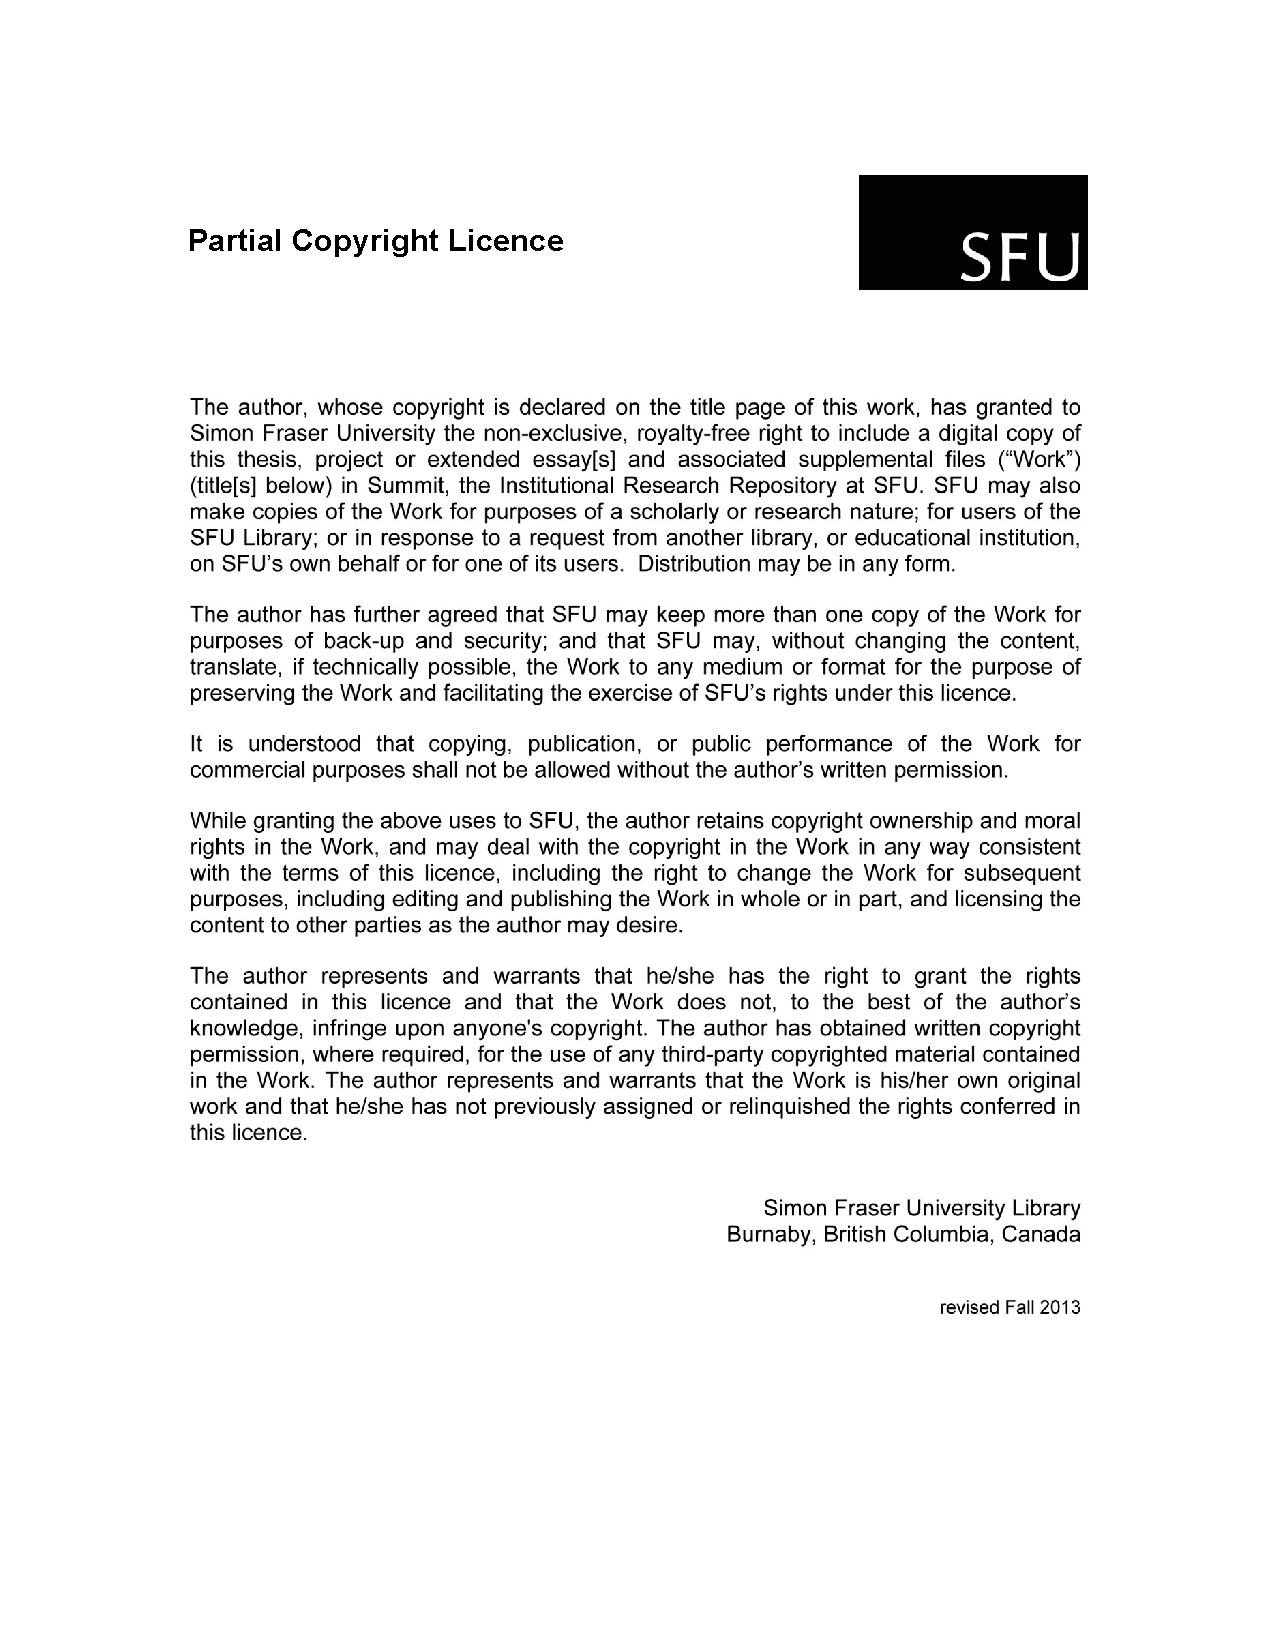
\includegraphics{PCL_Declaration.pdf}
	}
}
\makeatother
\newpage

%% Copyright 1998 Pepe Kubon
%%
%% `abstract.tex' --- abstract for thes-full.tex, thes-short-tex from
%%                    the `csthesis' bundle
%%
%% You are allowed to distribute this file together with all files
%% mentioned in READ.ME.
%%
%% You are not allowed to modify its contents.
%%

%%%%%%%%%%%%%%%%%%%%%%%%%%%%%%%%%%%%%%%%%%%%%%%%%
%
%       Abstract
%
%%%%%%%%%%%%%%%%%%%%%%%%%%%%%%%%%%%%%%%%%%%%%%%%

\prefacesection{Abstract}

TODO --- very rough --- from a proposal

% 350 words

In my first chapter, I review the application of financial portfolio theory to
ecology. I review the three contrasting applications: metaphors to communicate
the benefit of biological diversity, metrics to compare the benefits of
diversification across systems and time, and management tools to make robust
conservation decisions in the face of environmental uncertainty. I highlight
issues with applying portfolio theory to ecology (e.g. how we 'invest' in
financial and ecological portfolios can fundamentally differ and ecological
data presents new statistical issues) and outline key questions for the field
to address.

In my second chapter, I evaluate two methods for estimating the ecological
portfolio effect and apply these methods to metapopulation data from around the
world across moths, reef fishes, and salmon. I show an inherent bias to a
commonly applied method, outline recommendations for researchers when
estimating ecological portfolio effects, and show that the general tendency is
for stabilizing ecological portfolio effects.

In my third chapter, I show how a portfolio approach to managing population
diversity can inform conservation priorities for salmon populations under a
changing climate. My findings suggest the importance of conserving the
processes that promote thermal-tolerance diversity, such as genetic diversity,
habitat heterogeneity, and natural disturbance regimes, and demonstrate that
diverse natural portfolios may be critical for metapopulation conservation in
the face of increasing climate variability and change.

In my fourth chapter, I take the concept of heavy tails and black swans
(extreme and unexpected events) from the financial literature and ask what the
evidence is for these events in ecological abundance time series. I find strong
but rare evidence of ecological black swans across hundreds of populations from
around the world. When ecological black swans occur they tend to be associated
with extreme climate, parasites, predation, and interactions of these elements
with little relationship to life history. My proposed postdoctoral research
represents an extension of this topic.














 %% abstract
\include{dedquot} %% dedication and quotation, if any
%% Copyright 1998 Pepe Kubon
%%
%% `ack.tex' --- aknowledgments for thes-full.tex, thes-short-tex from
%%               the `csthesis' bundle
%%
%% You are allowed to distribute this file together with all files
%% mentioned in READ.ME.
%%
%% You are not allowed to modify its contents.
%%

%%%%%%%%%%%%%%%%%%%%%%%%%%%%%%%%%%%%%%%%%%%
%
%       Acknowledgment 
%
%%%%%%%%%%%%%%%%%%%%%%%%%%%%%%%%%%%%%%%%%%

\prefacesection{Acknowledgments}
Here go all the people you want to thank.








 %%  acknowledgments

%%%  generate contents, lists of figures, etc.
\lists

%% preface (foreword), if any
%%% Copyright 1998 Pepe Kubon
%%
%% `preface.tex' --- preface for thes-full.tex from
%%                   the `csthesis' bundle
%%
%% You are allowed to distribute this file together with all files
%% mentioned in READ.ME.
%%
%% You are not allowed to modify its contents.
%%

%%%%%%%%%%%%%%%%%%%%%%%%%%%%%%%%%%%%%%%%%%%%%%%%%
%
%       Preface 
%
%%%%%%%%%%%%%%%%%%%%%%%%%%%%%%%%%%%%%%%%%%%%%%%%

\prefacesection{Preface}
Here go all the interesting reasons why you decided to write this thesis.



%%% prepare main section
\beforetext

%%% main matter
\chapter[Introduction]{Introduction}

In the coming century we face a loss of biodiversity on the order of 100--10,000 times greater than average rates in the fossil record \citep{mea2005} --- a rate as fast if not faster than any of the five past mass extinctions \citep{barnosky2011, harnik2012}. Compounding this problem for conservation managers is uncertainty in future climate conditions \citep{heller2009} and the unknown responses of species and communities to those conditions \citep{lavergne2010}. Therefore, urgent questions are: Exactly how big a problem is the loss of biodiversity for the stability of ecological systems? How can conservation biologists communicate the insurance benefit of biodiversity to the public and policy makers? And, how can we apply limited conservation funds to manage biodiversity and limit risk in the face of increasing environmental uncertainty?

Nearly a decade ago, \citet{figge2004} and \citet{koellner2006} laid the foundation for why financial portfolio theory is ideally suited for answering these questions. Financial portfolio theory seems applicable to ecological systems for at least four reasons. First, ecological and financial systems are both structured hierarchically. Groups of populations form metapopulations and groups of species form communities; groups of financial assets form investment funds, which in turn form portfolios. Additionally, ecological and financial managers have similar goals. Ecological resource managers might wish to minimize the probability of population decline while maintaining an acceptable level of hunting of fishing; financial portfolio managers minimize the probability of large economic losses for an acceptable level of expected financial returns \citep{may2008}. Another reason why portfolio theory is ideally suited for ecology is that substantial resources have gone into developing mathematical theory for optimizing financial investments. There is therefore a rich body of theory and experience to draw from. Finally, the portfolio metaphor is an engaging and accessible way for ecologists and conservationists to think about ecological variance and biological diversity and convey the importance of this (often abstract) literature.

A number of recent studies have used financial portfolios as a metaphor, metric, or management approach (Fig.~\ref{fig:traits}) to estimate and communicate the stabilizing benefit of diversity and prioritize its conservation \citep[e.g.][]{schindler2010, ando2011, halpern2011, hoekstra2012, anderson2013, mellin2014}. For example, \citet{moore2010} used the portfolio metaphor to show how increased synchrony of salmon populations could lead to heightened extinction risk. \citet{thibaut2012} used the portfolio-effect metric to quantify the insurance benefit of diversity for reef fish communities. \citet{ando2012} used portfolio optimization to prioritize habitat for conservation that would create wetlands most robust to climate-change uncertainty. Portfolio theory promises to move conservation biology beyond the familiar concepts of the quantity, variety, and distribution of species \citep{mace2005} and into a new dimension that emphasizes elements of variance, covariance, stability, synchrony, and extremeness \citep{loreau2010a, thompson2013}.

\begin{figure}[htbp]
\centering
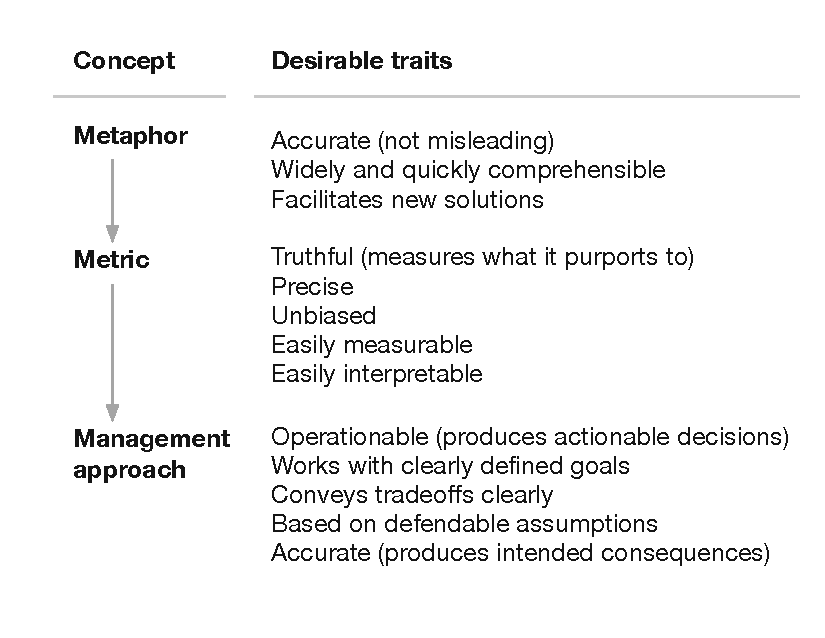
\includegraphics[width=4in]{mmm-traits.pdf}
\caption{Desirable traits of ecological metaphors, metrics, and management approaches
(decision-making tools).}
\label{fig:traits}
\end{figure}

But in applying financial theory to conservation biology, where does the portfolio metaphor break down? What exactly are the assets, portfolios, and investors in the financial metaphor? Furthermore, how might one invest in different kinds of ecological portfolios? And how might the differences between financial and ecological data affect our ability to apply financial portfolio theory to conservation biology? Are ecological portfolios just another name for existing ecological theory? Or, can ecological portfolios bring together and provide new insights into a wide variety of ecological theory?

TODO EDIT THIS!!! Here, we address these questions by reviewing the emerging literature on ecological portfolios. The purpose of our review is fourfold: review the three recent contrasting applications of ecological portfolios as metaphors, metrics, and management tools; illustrate how ecological portfolios can bring together a wide variety of modern ecological theory; highlight some challenges of applying financial theory to ecological portfolios; and emphasize the utility of portfolio optimization and risk metrics for conservation prioritization.

\section{Ecological portfolios as a metaphor}\label{ecological-portfolios-as-a-metaphor}

Metaphors are powerful tools for communicating and shaping scientific ideas \citep{brown2003} and are particularly useful in developing and communicating the field of conservation biology \citep{larson2011}. In conservation biology, the portfolio concept has long been used as a metaphor to emphasize the need to not put all your eggs in one basket. This metaphor has come into particular prominence in the last decade. For example, the IUCN Criterion B2a recognizes the risks associated with a species existing in few locations \citep{iucn2001}. As another example, ecologists have suggested the need to bet hedge by developping a portfolio of approaches when tackling conservation issues \citep[e.g.][]{ehrlich2008}. Ecologists have also used the metaphor to refer to diverse ecosystems and communities as portfolios of species \citep{figge2004}. These applications are an appealing way to convey concepts of diversification, uncertainty, and risk using familiar terminology.

\section{The portfolio-effect metric}\label{the-portfolio-effect-metric}

Beyond the metaphor, the portfolio-effect metric asks what the precise benefit is of a unit increase in diversity. The portfolio effect is derived from the economic question: How much better off are you by investing your money in a diversified portfolio instead of investing all your money in a single asset \citep{markowitz1952}? In conservation biology, we can consider the current ecological system the diversified portfolio and a theoretical homogeneous (or monoculture) system the single asset \citep{anderson2013}. For example, we could ask how much more stable is a metapopulation of salmon from different streams, rivers, or watersheds (the portfolio) compared to a theoretical homogeneous stream population (the single asset) \citep{schindler2010, carlson2011}. Hence, to accurately measure a portfolio effect we need to predict the variability of a theoretical homogeneous system---a system that lacks the element of biodiversity we are interested in. Unfortunately, although the portfolio metaphor provides a new way of looking at the decades-old diversity-stability debate, on its own it remains unclear whether it provides new insights about the nature of the relationship itself.

Nonetheless, by providing a new lens, the portfolio effect as a metric has created an impetus for new theoretical and empirical insights into stability-diversity relationships. Early work focused on theoretical aspects of the portfolio effect for greatly simplified systems---identifying when we would expect a stabilizing portfolio effect and what factors would enhance it \citep{doak1998, tilman1998, lehman2000}. Over time, theoretical studies developed indices that relaxed assumptions about the systems they describe \citep[e.g.][]{loreau2010a, thibaut2013, gross2013}. A recent trend has been to apply these indices to empirical data, albeit primarily to salmon \citep{greene2010, schindler2010, carlson2011, anderson2013, mellin2014}. However, empirical work has concentrated on applying relatively simple portfolio-effect metrics that make strong assumptions that are rarely met in empirical systems \citep{thibaut2013, anderson2013}. Violation of these assumptions, for example, the assumption that the temporal standard deviation scales directly with the mean, or that populations are approximately equal in size, can distort our perception of the portfolio effect and hence the perceived benefit of diversity to ecological stability \citep{anderson2013}.

\section{Ecological portfolio management}\label{ecological-portfolio-management}

In addition to measuring the portfolio-effect metric, we can use financial portfolio theory to inform decisions about conservation management. Markowitz's seminal contribution to financial portfolio theory was a focus on portfolio selection---the idea that out of all possible portfolios there exists a subset that maximize returns for a level of risk (or minimize risk for a level of return) \citep{markowitz1952} (Fig.~\ref{fig:mpt}). In conservation biology, the goals of conservation practitioners often parallel those of financial managers, even though they are rarely expressed as such \citep{figge2004}. We see ecological portfolio management happening in one of three ways: choosing existing management structures that promote diversified portfolios, using Modern Portfolio Theory (MPT) to optimize ecological resource extraction, or using MPT to optimize an ecological system itself.

\begin{figure}[htbp]
\centering
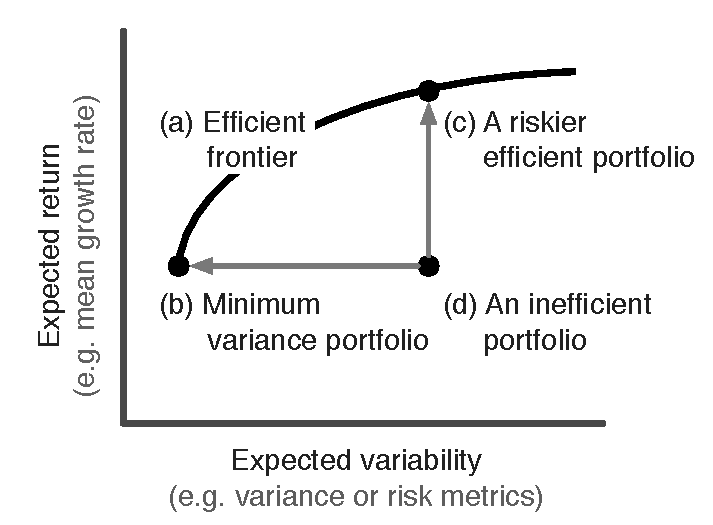
\includegraphics[width=3in]{efficient-frontier-fig.pdf}
\caption[An introduction to Modern Portfolio Theory mean-variance optimization.]{
An introduction to Modern Portfolio Theory mean-variance optimization. In
finance, portfolios are formed by choosing how much to invest in various
assets. Modern Portfolio Theory focuses on identifying the set of portfolios
that optimizes the trade-off between expected return (mean) and expected
variance or risk. (a) This set of portfolios is referred to as the efficient
frontier. (b) The minimum variance portfolio achieves the lowest expected
risk; the remaining risk is said to be undiversifiable. (c) A risker, but
still efficient portfolio. (d) An example inefficient portfolio, which has a
lower expected return than (c) and greater expected risk than (b). Adapted
from \citeauthor{hoekstra2012} (\citeyear{hoekstra2012}).
}
\label{fig:mpt}
\end{figure}

First, we can consider existing management structures that create systems analogous to diversified portfolios. For example, fishers can engage in catch-pooling cooperatives where fishers share the profits from their catches according to predefined rules. \citet{sethi2012} showed that this portfolio-like scheme reduces risk for red king crab fishers in the Bering Sea by up to 40\%. Other fisheries management tools, such as community-based management, individual transferable quotas (ITQs), and licensing systems that allow for fishing a diversity of species, can create diversified catch portfolios for fishers and buffer fishers against the risk of poor profits \citep{hilborn2001, kasperski2013}. Alternatively, we can consider the properties of a diversified portfolio, such as representation, resilience, and redundancy, and look for management strategies that promote these properties in ecological systems \citep{haak2012}

We can also use MPT directly to optimally allocate harvesting efforts. This suggestion is not new---some of the earliest references to ecological portfolios suggest portfolio theory as a management tool \citep{baldursson1997, costanza2000} but few studies have explored the idea to its full extent and interest in the topic has expanded strongly in recent years \citep[e.g.][]{edwards2004, sanchirico2008, halpern2011, moloney2011}. In conservation biology, portfolio optimization can be applied spatially. For example, \citet{halpern2011} used MPT to illustrate the tradeoff between fishing profits and spatial unevenness of marine resource value. MPT has also been used to optimize decisions about whether to clearcut or retain standing trees \citep{hyytiainen2008, hildebrandt2011}. As a third example, \citet{moloney2011} used MPT to optimize the choice of grazing animals on Australia's rangelands. With few exceptions, however, the application of MPT for harvesting decisions has been limited to fishery and forestry examples.

Finally, we can use ecological portfolio management to choose how we allocate conservation efforts to manage risk for an ecological system as a whole. For example, portfolio optimization can be used to spatially allocate conservation activity for wetlands to maximize ecosystem services at a given level of risk under the uncertainty of climate change \citep{ando2011, ando2012}. In forestry, MPT has been used to select the optimal weighting of seed sources for regenerating forests under a variety of climate change scenarios \citep{crowe2008}. In fisheries, MPT has been used to assess the risk-return trade-off for salmon metapopulation productivity given choices about what habitat to conserve under climate change and stream-flow reduction scenarios \citep{anderson2014}. We see this as a promising but largely unexplored use of ecological portfolio theory.

\section{Ecological theory to draw from}\label{ecological-theory-to-draw-from}

Portfolio theory can unite many existing ecological theories (Table~\ref{tab:theory}). For example, community ecology, the theory of island biogeography, metapopulation dynamics, and functional-group ecology can all generate portfolio-like ecological structure. Importantly, the portfolios produced by these scenarios have specific features that affect portfolio dynamics. For example, in community portfolios, predator assets can eat portions of prey assets, which has no direct equivalent in financial portfolios. In metapopulation portfolios, subpopulation assets can exchange individuals between each other and rescue subpopulation assets at low abundance or value.

Other ecological theories can inform expected patterns of diversification and portfolio dynamics (Table~\ref{tab:theory}). For instance, the Moran effect suggests that ecological assets that are further apart from each other are more likely to experience diverse environments and therefore provide greater portfolio diversification. The unified neutral theory of biodiversity and biogeography asks what we would observe if species were functionally equivalent. We can think of this neutral community as an undiversified portfolio and compare it to observed communities to examine the benefit of functional diversity. This comparison is analogous to the ecological portfolio-effect metric \citep[e.g.][]{doak1998, schindler2010, anderson2015}.

Finally, a variety of mechanisms can generate ecological portfolio diversification (Table~\ref{tab:theory}). For instance, intraspecific trait variation, response diversity, and even personality variation can be thought of as sources of portfolio diversification. Ecological portfolios therefore can have multiple levels of diversification, just as financial portfolios can be diversified across multiple levels such as investment types, geography, business sectors, and individual stocks. Whereas research on many of these ecological sources of diversification exists in its own niche, ecological portfolio theory encourages us to consider many elements in conjunction.

\LTcapwidth=\textwidth
\bibpunct{}{}{;}{a}{}{;}
%\singlespacing
\begin{small}
\begin{longtable}{>{\RaggedRight}p{3.6cm}>{\RaggedRight}p{7.3cm}>{\RaggedRight}p{3.6cm}}

\caption{Selected ecological theory relevant to ecological portfolios.}\\

\toprule

\textbf{Ecological theory} &
\textbf{Relevance to ecological portfolios} &
\textbf{Selected references} \\

\midrule
\multicolumn{2}{l}{\textbf{Sources of portfolio structure}} \\
\midrule

Community ecology &
We can represent species as assets and a community as a portfolio. Species interactions such as predation and competition may complicate the analogy. &
\citep{figge2004, morin2011}\\

Theory of island biogeography &
Explains a source of diversification for ``islands'', which have a portfolio-like structure. Larger islands may have higher levels of portfolio diversification. &
\citep{macarthur1967}\\

Metapopulations &
Subpopulations can act as diverse ecological assets as part of a metapopulation portfolio. Metapopulations usually have exchange between subpopulations (ecological assets), which may not have an analogy in financial portfolios. &
\citep{levins1969}\\

Functional groups &
Species that perform separate ecological functions can form ecological assets as part of an ecological portfolio. &
\citep{walker1992, thibaut2012}\\

\midrule
\multicolumn{2}{l}{\textbf{Causes of diversification and portfolio dynamics}}\\
\midrule

Moran effect &
Identifies that similar environments will induce similar population responses decreasing the diversity of a portfolio. Ecological assets that are further apart are expected to provide greater diversification. &
\citep{moran1949, ranta1998}\\

\bibpunct{(}{)}{;}{a}{}{} % add back brackets for in-text citation
Synchrony &
Often loosely used to referred to as correlation between ecological assets. Defined quantitatively by \citet{loreau2008} as a diversity-independent metric of correlation. The benefit of diversification is greater when synchrony of ecological assets is low. &%
\bibpunct{}{}{;}{a}{}{}%
\citep{ranta1998,moore2010,yeakel2014}\\

Unified neutral theory of biodiversity and biogeography &
Asks what community dynamics we would observe if species were functionally equivalent. We can think of a neutral community with ecological equivalence as an un-diversified portfolio compared to a diversified portfolio in which species show functional diversity. &
\citep{hubbell2001}\\

Biocomplexity &
Identifies that subpopulations can display a range of biological traits and behaviours and that these ranges can form portfolio diversification &
\citep{hilborn2003, hutchinson2008}\\

Response diversity &
Identifies elements of ecological systems that cause them to respond differently to perturbation. Potentially important aspect of ensuring stable portfolios as the magnitude and frequency of environmental stressors increase (e.g.\ climate change). &
\citep{elmqvist2003, loreau2008, loreau2013}\\

Intraspecific trait variation &
Identifies that variation among individuals in a population can form an important component of diversity and affect population dynamics. Individuals could be thought of as ecological assets. &
\citep{bolnick2011}\\

Spatial heterogeneity &
Heterogeneity in habitat may create pockets of diverse ecological assets. &
\citep{oliver2010,parn2012,mccluney2014}\\

%Compensatory dynamics and complementarity & … & [65]\\

%Competitive interactions & … & [37]\\

\midrule
\multicolumn{2}{l}{\textbf{Risk-reduction consequences of diversity}}\\
\midrule

Diversity-stability hypothesis &
Identifies when and why certain types of diversity correspond with certain types of stability. Another name for many of the same concepts that ecological portfolio theory addresses.  &
\citep{ives2007, loreau2013}\\

Statistical averaging &
Some level of reduction in variability in a portfolio is inevitable due to averaging of asset time series. &
\citep{doak1998}\\

Portfolio effect &
A term to represent the benefit of a system existing as a portfolio of ecological assets instead of a single homogeneous asset. &
\citep{tilman1998, schindler2010, thibaut2013, anderson2013}\\

Insurance hypothesis &
Similar to the portfolio effect, but emphasizes that negative covariance reduces the likelihood that all assets will decline at the same time. &
\citep{yachi1999,valone2008}\\

\bottomrule
\label{tab:theory}
\end{longtable}
\end{small}


TODO introduce the data chapters here

\bibliographystyle{apalike}\bibliography{/Users/seananderson/Dropbox/tex/jshort,/Users/seananderson/Dropbox/tex/ref3}

\chapter[Quantifying metapopulation portfolio effects]{Ecological
  prophets: Quantifying metapopulation portfolio effects\footnotemark{}}

\footnotetext{ A version of this chapter appears as Anderson, S.C., A.B.
  Cooper, N.K. Dulvy. Ecological prophets: Quantifying metapopulation
  portfolio effects. Methods in Ecology and Evolution. 4(10): 971-981.
  \url{http://doi.org/10.1111/2041-210X.12093}.}
\section{Abstract}
\begin{enumerate}
 \item A financial portfolio metaphor is often used to describe how population
   diversity can increase temporal stability of a group of populations. The
   portfolio effect (PE) refers to the stabilizing effect from a population
   acting as a group or ``portfolio'' of diverse subpopulations instead of a
   single homogeneous population or ``asset''. A widely used measure of the PE
   (the average-CV PE) implicitly assumes that the slope (z) of a log-log plot
   of mean temporal abundance and variance (Taylor's power law) equals two.

 \item Existing theory suggests an additional unexplored empirical PE that
   accounts for z, the mean-variance PE. We use a theoretical and empirical
   approach to explore the strength and drivers of the PE for metapopulations
   when we account for Taylor's power law compared to when we do not. Our
   empirical comparison uses data from 51 metapopulations and
   1070 subpopulations across salmon, moths, and reef fishes.

 \item Ignoring Taylor's power law may overestimate the stabilizing effect of
   population diversity for metapopulations. The disparity between the metrics
   is greatest at low z values where the average-CV PE indicates a strong PE.
   Compared to the mean-variance method, the average-CV PE estimated a stronger
   PE in 84\% of metapopulations by up to seven-fold. The divergence between
   the methods was strongest for reef fishes ($1.0 < \text{z} < 1.7$) followed
   by moths ($1.5 < \text{z} < 1.9$). The PEs were comparable for salmon where
   $\text{z} \approx 2$.

 \item We outline practical recommendations for estimating ecological PEs based
   on research questions, study systems, and available data. Since most PEs
   were stabilizing and diversity can be slow to restore, our meta-analysis of
   metapopulations suggests the safest management approach is to conserve
   biological complexity.

\end{enumerate}

%\noindent
%\textit{Key-words}: Allee effect, biocomplexity, Great Barrier Reef, Moran
%effect, population diversity, response diversity, stability, synchrony

\section{Introduction}

Biological complexity is increasingly recognized as a critical factor
underpinning the stability of ecological systems
\citep[e.g.][]{hilborn2003, ives2007, schindler2010}.
While the diversity-stability relationship for ecosystem properties is
generally held to be true, what is not known is the relative increase in
benefit from each additional element of biodiversity for stability and
persistence \citep{cardinale2012}. For example,
\citet{schindler2010} found that sockeye salmon populations in Bristol Bay
were twice as stable as a homogeneous population and management should focus on
retaining biological diversity to ensure a ten-fold reduction in the frequency of
fishery closures. The stabilizing benefit of such population diversity is
clearly a critical and undervalued component of ecological systems for resource
management to conserve, yet there are few ways to quantify its benefit.

The empirical portfolio effect (PE) is a rapidly popularized metric
\citep[e.g.][]{schindler2010, carlson2011, iMCC2011} derived from
theory introduced a decade earlier \citep{doak1998, tilman1998,
tilman1999} that aims to measure the increase in stability due to
subpopulation diversity within a metapopulation (or greater species diversity
within a community). For example, we can think of salmon from individual streams
as assets (subpopulations) within a portfolio (metapopulation) that comprises
the watershed. If subpopulations react differently to environmental
variability, then the metapopulation may experience a reduced risk of collapse
or decline. Similarly, financial managers choose portfolios of diverse
financial assets to reduce their risk of financial losses.

Financial managers estimate the benefit of diversifying a
financial portfolio by comparing the variability in returns from investing in a
single asset to the variability from investing in a diversified portfolio
\citep{markowitz1959}. In ecology, the empirical PE has been calculated by
comparing the temporal coefficient of variation (CV) of metapopulation abundance
(the diversified portfolio; Fig.~\ref{fig:didactic}a) to the average CV of
subpopulation abundances (the single assets; Fig.~\ref{fig:didactic}b)
\citep{secor2009, schindler2010, carlson2011}. We refer to this
approach as the \index{average-CV PE}average-CV PE (Fig.~\ref{fig:didactic}c). But ecological and
financial systems differ; it is timely to consider whether we can apply the same
approach to ecological systems.

One crucial difference between financial and ecological portfolios is how asset
variability scales with investment. For a financial asset, the standard
deviation of an investor's returns increases linearly with investment because
investing in a financial stock doesn't meaningfully affect the stock's
properties. Therefore, as mean financial investment increases, we expect the
variance in returns to increase by a power of two. This is not true in
ecological systems. As abundance of a subpopulation grows (i.e.\ as investment
in the single asset grows), the standard deviation usually increases
nonlinearly according to \index{Taylor's power law}Taylor's power law: the slope (z) of a log-log plot of
the variance and mean of subpopulation abundance is typically less than two
\citep{taylor1980,taylor1982}. This means that larger populations may
be less variable than expected if we applied the financial metaphor. The
CV is not necessarily a size-independent metric of variability
\citep{mcardle1990}.

The theoretical work of \citet{tilman1998} implies an alternative way to
measure the empirical PE that accounts for the mean-variance relationship.
Rather than assuming we can represent the variability of the theoretical
homogeneous metapopulation (the single asset) by the average subpopulation CV,
we can estimate the variance of the homogeneous metapopulation by extrapolating
the mean-variance relationship to the observed metapopulation size
(Fig.~\ref{fig:didactic}d). We can then compare this expected
homogeneous-population variability to the observed metapopulation variability
to get what we call the \index{mean-variance PE}mean-variance PE. This mean-variance PE asks: If the
mean-variance relationship continued to scale as we observed for larger and
larger subpopulations, how much more variable would we expect the
metapopulation to be if it was identically sized but acted with the same
dynamics as any one subpopulation? Therefore, although both the mean-variance
PE and the average-CV PE get at the benefit of splitting one large population
into many subpopulations, only the mean-variance PE accounts for the observed
mean-variance scaling relationship --- the average-CV PE assumes that z~=~2.
Given this theoretical advantage of the mean-variance PE, what happens when we
apply the average-CV PE to empirical data where z is typically less than two,
as recent literature has done \citep{secor2009, schindler2010,
  carlson2011}?

Here, we conducted the first large-scale cross-taxa evaluation of the
average-CV PE compared to the mean-variance PE for metapopulations,
specifically addressing three main questions: (1) How does the average-CV PE
differ compared to the mean-variance PE when applied to theoretical systems
with varying z values? (2) How prevalent and strong is this difference across
51 metapopulations and 1070 subpopulations of
salmon, moths, and reef fishes? (3) Despite its stronger theoretical
foundations, is the mean-variance PE a reliable empirical metric of how
subpopulation diversity benefits stability? We conclude with a guide to
measuring metapopulation PEs based on question, study system, and data type.

\section{Materials and methods}

\subsection{Defining the metapopulation portfolio}

In our finance-ecology metaphor we represent portfolio value as
metapopulation abundance and financial-asset value as subpopulation abundance.
We define metapopulations\index{metapopulations} as groups of \index{subpopulations} that behave largely
independently but are linked by dispersal of individuals among subpopulations
\citep{levins1969}.
Although our data represent subpopulations in the spatial-metapopulation
sense, the methods in this paper could be applied more broadly.
For example, future studies could consider different age classes, different
life-history variants, or populations with different thermal-tolerances as
subpopulations.
Although the PE has also been applied to multiple species within a
community \citep[e.g.][]{doak1998, tilman1998, karp2011}, and
elements of our analysis are applicable to community portfolio effects, the
analysis of PEs in communities is complicated by trophic interactions, changes
in mean abundance with increasing diversity (the over-yielding effect), and
differing mean-variance scaling relationships across species
\citep[e.g.][]{loreau2010, thibaut2013}.

When discussing the properties of metapopulation portfolios we use
three terms (stability, diversity, and homogeneous population), which we define
here.
We define \textit{stability}\index{stability} in terms of the variability (CV) of population
trajectories through time.
We define \textit{subpopulation diversity}\index{subpopulation} as the asynchrony (lack of
correlation) between the groups defined as subpopulations.
Since our metrics are phenomenological, they don't specify the mechanism
generating asynchrony, but a central candidate would be diversity of response
to environmental fluctuations
\citep[e.g.][]{elmqvist2003,loreau2008,thibaut2012}.
We define a \textit{homogeneous population}\index{homogeneous population} as a theoretical population the
same size as the existing ``diverse'' population but lacking whatever
subpopulation diversity we are measuring. For metapopulations we can think of
this in one of two ways: (1) a population the same size as the metapopulation
that behaves like the average subpopulation or (2) a metapopulation with synchronized
subpopulation dynamics.

\subsection{Theoretical evaluation of portfolio effects}

We defined the PE\index{portfolio effect} as the ratio of the CV of a theoretical system composed of a
single subpopulation or asset ($\CV_a$) to the observed metapopulation or
portfolio CV ($\CV_p$). A PE of two, for example, would indicate that a
metapopulation is two times less variable than if it were comprised of a single
homogeneous population. For uncorrelated subpopulations and $\sigma^2 = c
\mu^z$ (where $\sigma^2$ is the temporal variance, $\mu$ is the temporal mean,
and $c$ is a constant that doesn't affect the PE and is hereafter ignored for
simplicity), both interpretations of the PE define $\CV_p$ for subpopulations
$i$ 1 through $n$ as
\begin{equation}
\CV_p = \dfrac{\sqrt{{\mu_i}^z + {\mu_{i+1}}^z + \ldots + {\mu_n}^z}}{\mu_i +
\mu_{i+1} + \ldots + \mu_n}.
\label{eq:prophets:1}
\end{equation}

\noindent The average-CV PE defines $CV_a$ as
\begin{equation}
\CV_a = \dfrac{\dfrac{\sqrt{{\mu_i}^z}}{\mu_i} +
\dfrac{\sqrt{{\mu_{i+1}}^z}}{\mu_{i+1}} + \ldots +
\dfrac{\sqrt{{\mu_n}^z}}{\mu_n}}{n},
\label{eq:prophets:2}
\end{equation}

\noindent whereas the mean-variance PE defines $\CV_a$ as
\begin{equation}
\CV_a = \dfrac{\sqrt{(\mu_i + \mu_{i+1} + \ldots + \mu_n)^z}}{\mu_i +
\mu_{i+1} + \ldots + \mu_n}.
\label{eq:prophets:3}
\end{equation}

\noindent Equations \ref{eq:prophets:2} and \ref{eq:prophets:3} are equal if $z = 2$.

To extend the theoretical PE calculations to metapopulations with $\rho$
correlation between subpopulations, we can calculate the metapopulation or
portfolio variance $\sigma^2_p$ as

\begin{equation}
 %\sigma^2_p = \sum_{i =1}^n \sigma^2_i + \sum_{i =1}^n \sum_{\substack{j =1 \\
  %j \neq i}}^n \rho \sqrt{\sigma^2_i \sigma^2_j}.
 \sigma^2_p = \sum_{i =1}^n \sigma^2_i + \sum_{i =1}^n \cdot \sum_{j =1}^n \rho \sqrt{\sigma^2_i \sigma^2_j}. (4)
\end{equation}

We explored the implications of the two PE definitions across four statistical
properties that are ecologically meaningful and have precedence in the PE
literature \citep{tilman1999, cottingham2001, loreau2010,
thibaut2013}: the correlation between subpopulations, the temporal
mean-variance scaling relationship (z), the number of subpopulations, and the
evenness of subpopulation mean abundance. The expected effect of these
properties on  stability
has been addressed in the literature cited
above. Our focus, instead, is to understand the performance of the average-CV
method compared to the mean-variance PE across these four ecological
attributes. We show that differences between these PE metrics arise in
real-world metapopulations, and for each taxon we diagnose the ecological
reasons why the differences arise.

\subsection{Empirical evaluation of portfolio effects}

\subsubsection{Data sources}

To test the real-world strength of the average-CV and mean-variance PEs, we
collected metapopulation time-series data for salmon, moths, and reef fishes
(Table~\ref{tab:datasources}; Figs~\ref{fig:ts},~\ref{fig:map}).
We obtained salmon returns from the primary
literature, in particular \citet{dorner2008}, and government research
documents (Table~\ref{tab:datasources}). We obtained moth abundance trends from
the Rothamsted Insect Survey \citep{conrad2004}. These data represent
univoltine moths captured by light traps. We obtained reef visual census fish
counts from the Australian Institute of Marine Science Long-term Monitoring
Program \citep{sweatman2008}. See Tables~\ref{tab:ris-meta} and
\ref{tab:grb-meta} for the subpopulation site locations of the moth and reef
fish populations, respectively. Details on our data sources are available in the
Supporting Information.

We defined data inclusion criteria to ensure adequate estimation of temporal
mean-variance relationships. For salmon and moths we excluded populations
with less than four subpopulations or ten years of data and where the largest
subpopulation temporal mean was less than three times the size of the smallest
temporal mean. To reduce the number of reef fish populations to an
approximately comparable number, we used the metapopulations used by
\citet{mellin2010}. Their main inclusion criteria were five
subpopulations, 15 years of data, and two orders of magnitude difference in
subpopulation means.

\subsubsection{Average-CV PE}

We calculated the empirical average-CV PE\index{average-CV PE} as the ratio of the mean subpopulation
CV to the observed metapopulation CV (Fig.~\ref{fig:didactic}c). We estimated
confidence intervals by bootstrap; we sampled the subpopulations within each
metapopulation 500 times, with replacement, and recalculated the PE. We then
used the adjusted bootstrap percentile (BCa) 95\% confidence intervals
\citep{canty2012}.

\subsubsection{Mean-variance PE}

To calculate the empirical mean-variance PE\index{mean-variance PE}, we estimated z as the slope of a
linear regression of the subpopulations' ($i$) interannual log($\sigma^2$) and
log($\mu$),
\begin{equation}
  \log(\sigma^2_i) = \beta_0 + z \cdot \log(\mu_i) + \epsilon_i (5)
  \label{eq:linear-taylor}
\end{equation}

\noindent where $\epsilon_i$ represents independent and identically distributed
residual error with mean zero and an estimated variance. We used this model to
predict the variance given the mean of the metapopulation abundance
($\hat\sigma^2$; Fig.~\ref{fig:didactic}d). The $\hat\sigma^2$ reflects the
variance we would expect if the portfolio was composed of a homogeneous
population. We then calculated the mean-variance PE as the ratio of
observed $\sigma^2$ to predicted $\hat\sigma^2$. The mean-variance PE is
therefore equivalent to
the average subpopulation CV adjusted for the observed subpopulation CV
mean-variance scaling relationship.
We obtained confidence intervals on the mean-variance PE by
re-calculating the PE using the 95\% confidence intervals on the predicted
metapopulation variance.

Our empirical mean-variance PE calculation assumes the inter-subpopulation
mean-variance relationship can be used as a proxy for the intra-subpopulation
relationship. To test this we estimated the intra-subpopulation mean-variance
relationship between the first and second halves of the subpopulation time
series for the time-series in which one half was at least two-times greater. We
compared these intra-subpopulation z values with the inter-subpopulation z
values used in our analysis.

\subsection{Alternative ways of extrapolating the mean-variance PE}

\textit{Quadratic extrapolations}: In our main analysis, we estimated Taylor's
power law z values by linear regression of the time-series' log-transformed mean
and variance values. In some cases, a quadratic fit may be more appropriate
\citep{routledge1991, perry1992}. We fit a quadratic model,

\begin{equation}
  \log(\sigma^2_i) = \beta_0 + \beta_1 \log(\mu_i) + \beta_2 \log(\mu_i)^2 +
  \epsilon_i, \quad \beta_2 \ge 0. (6)
  \label{eq:quad-taylor}
\end{equation}

\noindent
\citet{perry1992} suggest limiting the lower value of $\beta_2$ to 0 since
a negative $\beta_2$ would imply that at some value of $\mu$ the $\sigma^2$
would decrease with increasing $\mu$ and eventually become negative. We used
the R package \texttt{nls} \citep{r2013} with the \texttt{port} algorithm
to fit the quadratic model and bound the lower value of $\beta_2$ to 0. If
$\beta_2 = 0$ the quadratic model simplifies to the linear model.

\textit{Model averaging}: Whereas the quadratic version of Taylor's power law
can only provide a closer fit to the data than the linear version due to the
added coefficient, it does so at the expense of greater model complexity and
potentially poorer predictive capacity. We also examined predictions averaged
across the linear and quadratic models with the predictions weighted by the
Akaike weights of their respective models \citep{burnham2002}. We fit an
AICc-model-averaged version of the linear and quadratic Taylor's power law fits
using the R package \texttt{MuMIn} \citep{barton2012}.

\subsection{Accounting for non-stationary time-series}

Long-term trends in data can upwardly bias variability metrics such as the CV.
We therefore conducted two alternative analyses in which we detrended
the data before estimating the PEs. We used the residuals from (1) a fitted
linear model and (2) a fitted loess smoother \citep[\texttt{loess}
function;][]{r2013} with a smoothing span of 75\% of the data. For both
the subpopulations and metapopulations we calculated the mean abundance before
detrending. We estimated the variance of each subpopulation using the detrended
time-series. We estimated the variance of the metapopulations using the
detrended version of the original metapopulation abundance time-series.
A more thorough analysis of PEs for non-stationary time series might
consider the distribution of means, variances, and CVs within each
subpopulation, but was beyond the scope of our analysis.

\subsection{The \texttt{ecofolio} R package}

We provide an R package \texttt{ecofolio} to estimate the PEs described in this
paper (see the Supporting Information). In addition to the average-CV and
mean-variance PEs, our package includes options to fit quadratic mean-variance
scaling models, average across mean-variance model predictions, and detrend
non-stationary time-series.

\section{Results}

\subsection{Theoretical evaluation of portfolio effects}

By assuming z = 2, the average-CV method can misrepresent the effect of changes
in subpopulation number, correlation, and evenness on the PE
(Fig.~\ref{fig:lines}). The average-CV PE universally becomes more stabilizing
(higher PE) as subpopulation number increases regardless of z, whereas
when we account for the mean-variance relationship, the PE can become
destabilizing with more subpopulations at small z values
(Fig.~\ref{fig:lines}a). The PE becomes less stabilizing as correlation
increases regardless of the method, although accounting for the mean-variance
relationship shifts the PE uniformly (assuming even subpopulation sizes) across
all correlation values (Fig.~\ref{fig:lines}b). The average-CV PE can
erroneously become more stabilizing as subpopulations become uneven; the
mean-variance PE indicates that the PE would become less stabilizing at high z
values or remain relatively constant at low z values (Fig.~\ref{fig:lines}c).

\subsection{Empirical evaluation of portfolio effects}

The key assumption that ecological systems have the same mean-variance
relationship as financial systems (z = 2) does not hold across
taxa. Whereas z was not significantly different from two for
17/20 of the salmon metapopulations,
there was infrequent overlap between the 95\% CI and two for the moth
metapopulations (3/20), and no overlap for
reef fish metapopulations (Figs~\ref{fig:Taylor-fits}, \ref{fig:z-vals}). The
inter-subpopulation mean-variance relationship was a reasonably unbiased proxy
for the intra-subpopulation mean-variance relationship. The slope of a
regression of median intra- and inter-subpopulation z was 1.04 (95\% CI:
0.51--1.57) although there was a high degree of scatter ($R^2 = 0.25$;
Fig.~\ref{fig:inter-vs-intra-z}).

In our empirical meta-analysis, the PEs varied strongly between, but also
within, taxonomic groups due to the mean-variance scaling
(Fig.~\ref{fig:meta}). The mean-variance PE ranged from
0.5--2.0 and the average-CV PE from
0.8--6.3. Hence, at best the
mean-variance PE suggests the metapopulation portfolio is twice as stable as
the homogeneous single asset. In comparison, the average-CV PE suggests the
metapopulation portfolio could be up to six times more stable. The z values
varied by taxonomic group, with the highest observed for salmon populations and
the lowest for reef fishes. As z decreased (reading from top to bottom) the
average-CV PE indicated increasingly stabilizing PEs compared to the
mean-variance PE (Fig.~\ref{fig:meta}a). For salmon, where the z values tended
to be near two, the PE metrics were largely in agreement (Fig.~\ref{fig:meta}a,
b). By contrast, for reef fishes, where the z values were small (mean =
1.3, range = 1.0--1.7),
the meta-analytic average-CV PE indicated a substantially more stabilizing PE
(mean = 3.6,
3.2--4.3 95\% CI) than the
mean-variance PE (mean = 0.9,
0.8--1.0 95\% CI) (Fig.~\ref{fig:meta}a,
d). The dashed-red lines in Fig.~\ref{fig:meta}b--d illustrate the
mean-variance fit if z is assumed to equal two as in the average-CV PE. Whereas
the mean-variance relationship assumed by the average-CV appears reasonable for
salmon (Fig.~\ref{fig:meta}b), it deviates strongly from the observed
relationship for some moth and reef fish metapopulations (Fig.~\ref{fig:meta}c,
d).

The mean-variance PE was highly sensitive to the estimation method
(Fig.~\ref{fig:detrend}). In particular,
13/18 reef fish metapopulations
switched from destabilizing to stabilizing PEs with quadratic
(Fig.~\ref{fig:meta-quad}) or quadratic-linear averaged
(Fig.~\ref{fig:meta-lin-quad-avg}) models. The AICc of the quadratic models was
lower in 11/51 metapopulations and at least two
units lower in 8/51, indicating
increased support despite the added model complexity. Linear
detrending generally created a similar mean-variance PE pattern to the original
mean-variance PEs (Figs~\ref{fig:detrend}, \ref{fig:meta-detrend}). Loess
detrending increased the mean-variance PE in
34/51 cases and the average-CV PE
in 34/51, lowering it in the
others (Figs~\ref{fig:detrend}, \ref{fig:meta-detrend-loess}). None of the
detrending options or alternative mean-variance extrapolations resulted in a
similar pattern for both the mean-variance and average-CV PE.

\subsection{Diagnosing the ecological properties of empirical portfolio effects}

Plotting the empirical metapopulations in the theoretical PE parameter space
revealed five key findings (Fig.~\ref{fig:paramspace}).
(1)~By viewing the coloured shading of the panels from left to right, we
can see that the average-CV PE responds inversely to z compared to the
mean-variance PE, and this issue is prevalent for the parameter space observed
in real ecological systems.
(2)~The empirical PEs were strongly grouped by taxonomy (see also
Fig.~\ref{fig:paramspace-labels}).
(3)
%There were regions of the parameter space not occupied by empirical
%metapopulations;
We did not observe metapopulations that were both highly
uneven and highly correlated (lower-right panels of Fig.~\ref{fig:paramspace}).
(4)~The PE surface surrounding the observed metapopulations (the colour
shading) was highly sensitive to changes in z for the mean-variance method when
correlation was low (e.g.\ Fig.~\ref{fig:paramspace}b), but the corresponding
surface of the average-CV PE for the same metapopulations was insensitive to
changes in z (e.g.\ Fig.~\ref{fig:paramspace}k).
(5)~The average-CV method,
however, considerably overestimated the PE compared to the mean-variance PE for
uneven metapopulations with small values of z (Fig.~\ref{fig:paramspace}c
versus \ref{fig:paramspace}l).
%however, became highly sensitive to z if unevenness
%was high (Fig.~\ref{fig:paramspace}l). Many metapopulations were uneven enough
%(and z was small enough) that the average-CV considerably overestimated the PE
%compared to the mean-variance PE (Fig.~\ref{fig:paramspace}c versus
%\ref{fig:paramspace}l).

Predicting the PE using these four properties alone (binned as shown in
Fig.~\ref{fig:paramspace}) explained
84\% of the variability in the average-CV PE and
53\% of the mean-variance PE ($R^2$ from a regression
of log theoretical PE and log empirical PE;
Fig.~\ref{fig:PE-predicted-observed}). The factors driving the PE co-varied; in
particular, we observed high correlation of subpopulations associated with high
variability (CV) and few subpopulations (Fig.~\ref{fig:factors-cor}b, c). High z
values occurred when there were few moderately-to-highly correlated
subpopulations (Fig.~\ref{fig:factors-cor}e, f).

\section{Discussion}

We conclude that the empirical average-CV PE is incompatible with Taylor's power
law and, due to the parameter space in which most ecological populations exist,
will tend to estimate a stronger benefit of population diversity than the
mean-variance PE. In this discussion, we begin by considering the influence of
mean-variance scaling on subpopulation and metapopulation stability and the
possible mechanisms behind stabilizing portfolio effects.
We then review limitations of these phenomenological metrics and discuss the
potential of mechanistic models. We conclude by synthesizing our results into
practical recommendations for quantifying ecological PEs.

\subsection{The influence of mean-variance scaling}

The primary difference between the mean-variance and average-CV PEs is how they
depend on z. The mean-variance PE becomes more stabilizing with increasing z.
The average-CV PE does the opposite (or remains constant) because the theory
assumes z = 2 and the measures increasingly diverge as empirical populations
deviate from this value. An increased z value (with all else being equal) means
that all subpopulations are more variable \citep{mellin2010}, but it also
increases the benefit of a portfolio structure \citep{tilman1998,
tilman1999, cottingham2001}. This subtlety highlights a potential
source of confusion: the PE is a relative measure comparing two sources of
variability. It does not reflect the absolute stability of the portfolio or of
the theoretical homogeneous portfolio. The stability of these components could
decline while the PE increases. In some scenarios, we can think of the
mean-variance PE as a consolation prize for a higher z value --- the
subpopulations become less stable and the metapopulation becomes less stable,
but the stabilizing effect of diversity increases.

Why is z usually less than two?
Explanations tend to fall into one of three categories. First, the most common
explanation is demographic stochasticity. Demographic stochasticity has been
implicated via simple stochastic population growth models
\citep[e.g.][]{anderson1982, ballantyne2005} and may be a
particularly strong driver when density dependence generates chaotic dynamics
\citep{perry1994}. In simplified theoretical systems, z will tend towards
two under conditions that increase population synchrony (such as strong
environmental forcing) and tend towards one under conditions that decrease
synchrony (such as strong demographic stochasticity) \citep{loreau2010}.
Second, competitive species interactions can affect z values.
\citep{kilpatrick2003}. For example, if competition with other species
impacts larger populations less than smaller populations, then z
will be less than two. Third, measurement error in abundance estimates
\citep{perry1981}, and particularly rounding at low abundance
\citep{taylor1982}, can create artificially low z values. However, it
remains unclear which of these three explanations, under what conditions, are
responsible for observed z values across real ecological systems. Further, z can
depend on the spatial and temporal scale of analysis \citep{leps1993} and
most existing theories do not explain why z could be greater than two as
we observed in 8/51 of our metapopulations and other experimental and
observational studies have observed \citep[e.g.][]{valone2003}.

In financial systems, analysts use the equivalent of the average-CV PE to
calculate the benefit of diversifying a financial portfolio. For such systems,
the approach makes sense since the standard deviation of investment value should
scale directly with investment (z = 2). For example, if a financial investor
triples investment in an asset, the investor can expect the standard deviation
of the returns from that investment to triple. Similarly, the average-CV PE may
be an appropriate method if applied to analogous questions about natural
resource extraction. For example, we can ask how stable a fisher's catches would
be if the fisher targeted a diverse portfolio of stocks instead of a single
stock. Here, the analogy is more straightforward: the fisher (the investor)
invests time, effort, and resources into fishing a fish stock (the asset) or
multiple fish stocks (the portfolio) and catches are returned. Given moderate
levels of fishing and ignoring issues related to efficiency, any one fisher
will not change the mean-variance properties of the fish stock and hence the
average-CV PE will be appropriate.

The PE metrics in this paper compare the observed metapopulation variability to
the theoretical variability of a single homogeneous population. This
homogeneous-population reference point is the most direct interpretation of the
financial portfolio analogy --- a financial investor can invest all her money
in a single asset (our reference point) or in a diversified portfolio (our
comparison). This homogeneous-population reference point is loosely equivalent
to the monoculture reference point often used in community PE analyses
\citep[e.g. Equation 7 in][]{thibaut2013}. However, other reference points
may be more relevant to ecology and easier to test experimentally. For example,
researchers might instead choose as a reference point metapopulation variance
under a harvesting regime that tends to synchronize subpopulations or
metapopulation variance if habitat loss eliminated certain subpopulations.

\subsection{Mechanisms driving metapopulation portfolio effects}

Two major mechanisms may generate stabilizing metapopulation PEs.
First, diversity of phenotypes across subpopulations can cause subpopulations
to react differently to the same environmental forces \citep[response
diversity;][]{elmqvist2003}. Second, since metapopulations can exist over
a large area, subpopulations may experience a greater diversity of
environmental conditions than an individual population (i.e.\ Moran effect). In
contrast, non-systematic sources of variability such as demographic
stochasticity should not generate stabilizing PEs \citep{loreau2008}. Our
results suggest a research agenda that seeks to understand the relative
contribution of these mechanisms across taxa and geography and the ecological
management approaches that can promote stabilizing PEs.

We observed a number of PEs less than one. These PEs indicate the
metapopulations would theoretically be less variable as one large homogeneous
population than as the product of many small subpopulations. These have been
referred to as inverse PEs \citep{thibaut2013}, and documented in other
observational studies \citep{deClerck2006}.
One explanation for these inverse PEs could be increased
demographic stochasticity at low population densities resulting in an Allee
effect \citep{allee1931}. Further, \citet{minto2008} demonstrated an
increase in the variability of fish offspring survival at low population
densities. The same sized metapopulation split into fewer subpopulations might
avoid these effects. A second explanation for these apparent inverse PEs
could involve hidden diversity. Other elements of diversity, such as size and
age structure, can be reduced at low population densities
\citep[e.g.][]{hutchings1993}. Therefore, inverse PEs could arise if the
diversity we are measuring (subpopulation number) increases but the unmeasured
diversity within the subpopulations decreases. This hidden diversity may be
more relevant to stability.

\subsection{Limitations of phenomenological portfolio effects}

Beyond tending to overestimate the benefit of diversity if z $<$ 2, there are
potential consequences to applying the average-CV as an ecosystem index. First,
the average-CV PE could fail to prioritize conservation of populations most in
need. For example, if we consider two otherwise similar metapopulations, the
average-CV PE will always be the same or stronger for metapopulations divided
into more subpopulations. However, the mean-variance PE indicates that there is
a threshold at which subdivision no longer benefits metapopulation stability
(Figs~\ref{fig:lines}a, \ref{fig:paramspace}a--i, \ref{fig:PE-as-an-index}).
Second, used as an ecosystem index through time, the average-CV PE could fail to
warn us of critical change or create the false impression of recovery. For
example, if a reef fish metapopulation with a low z value and moderate evenness
(circles in Fig.~\ref{fig:paramspace}k) became more uneven in mean subpopulation
size (see Fig.~\ref{fig:paramspace}l) the average-CV PE would become up to about
five times more stabilizing. The mean-variance PE informs us, however, that a
change in evenness has little influence on the portfolio effect in this
parameter space (Fig.~\ref{fig:paramspace}b~cf.~c).

Despite its stronger theoretical foundations, we emphasize caution when
interpreting empirical mean-variance PE values for reasons related to model,
biological, and measurement uncertainty. \textit{Model uncertainty}: Is a
log-log mean-variance linear model always best supported by the data?  We often
observed non-linearities in the relationship and studies have suggested numerous
other mean-variance models (e.g.\ quadratic models,
\citealt{routledge1991}; or models with a break-point at low population
abundance, \citealt{perry1992}).
\textit{Biological uncertainty}: Even if we knew the mean-variance model
precisely, will the same dynamics persist when extrapolating outside the range
of observed data?
\textit{Measurement uncertainty}:
%Even if we use the right model and the
%dynamics persist with extrapolation,
There may be biases in the estimated z values because of observation error
\citep{perry1981, taylor1982}, and estimates of z can depend on how
time-series are aggregated (here, what we define as a subpopulation)
\citep{fronczak2010}. Conclusions drawn from any phenomenological
mean-variance relationships should be tempered with caveats such as these.

The PE metrics measured in this paper are limited by the observational data to
which they are typically applied.
Recent mechanistic stability-diversity models that explicitly account for
asynchrony of response to environmental conditions exist
\citep[e.g.][]{ives2003, loreau2008, loreau2010,
demazancourt2013}
but are still largely unexplored beyond theory. However, mechanistic
stability-diversity models have at least two major problems. First, they must
assume a functional form to a mechanism and their results may be sensitive to
this decision. For example, does the environment affect productivity and does
productivity impact population growth rate through a Ricker or logistic growth
function? Second, the number of estimated parameters may exceed the power of
most ecological data sets \citep{thibaut2013}. Therefore, there remains a
need for phenomenological metrics.

\subsection{Practical recommendations for quantifying ecological portfolio effects}

Given the need for phenomenological PE metrics, which metric should you
chose? The answer depends on the research question and the scope of the
ecological system and data (Fig.~\ref{fig:recommendations}). \textit{Research
question}: The PE metrics discussed in this paper ask specifically how much more
stable the observed portfolio is than a theoretically homogeneous portfolio.
These metrics do not address the benefit of increases in portfolio size (e.g.\
metapopulation size) itself. In financial portfolio terms, these PE metrics address
the expected variability of a portfolio without addressing the expect rate of
return. \textit{Scope}: The average-CV or mean-variance PEs are relevant to any
portfolio-like aggregation in which the stability of the overall portfolio
``value'' is of interest and the interaction between ``assets'' is minimal. As
demonstrated in this paper, metapopulation abundance or biomass data can fall
into this scope. Other examples include fishers harvesting a portfolio of fish
stocks or a predator hunting a portfolio of species. These PE metrics
are not necessarily appropriate for a community of species where complications
such as multiple mean-variance relationships and trophic interactions may
require different phenomenological models \citep{thibaut2013}.

Assuming the research question, ecological system, and data are appropriate for
the methods shown in this paper, we recommend the following when choosing
between the average-CV and mean-variance PEs (Fig.~\ref{fig:recommendations}).
First, consider whether the mean-variance scaling relationship can be estimated.
Does a power law fit the data well? Are the subpopulations clearly defined? Is
there minimal observation error?

\begin{itemize}

  \item If the answer to any of these questions is no, then mean-variance
    scaling (z) is not well defined and you may need to ask a different question
    with a different metric. For example, you could quantify the synchrony of
    the populations using the synchrony index \citep{loreau2008,
    thibaut2013}.

  \item If $z \approx 2$ then use the average-CV PE, which amounts to the same
    metric as the mean-variance PE at $z = 2$ and is simpler to estimate,
    conceptualize, and communicate.

  \item If z is well defined but different than two then account for the
    mean-variance scaling relationship using the mean-variance PE.

\end{itemize}

The financial metaphor is an engaging and accessible way to convey the
importance of biological diversity to the public and provides a framework to guide
stability-diversity research \citep{figge2004, koellner2006}. However,
our results indicate the metaphor should be used with caution. By ignoring a
fundamental ecological property --- the mean-variance scaling relationship ---
the commonly applied average-CV PE method will tend to overestimate the benefit
of subpopulation diversity in real-world systems and may respond in
non-intuitive ways to ecosystem change.
Conversely, mechanistic stability-diversity models offer the gold-standard of PE
metrics but are challenging to apply in practice and so we still need phenomenological PE
metrics. Our results highlight the importance of
ground-truthing these metrics
and acknowledging their limitations.
Based on these results, our paper outlines practical recommendations
for estimating ecological PEs for metapopulations and similarly structured
ecological systems.
Irrespective of the challenges of finding a suitable metric to describe
the ecological PE,
given the tendency for stabilizing PEs and the challenges of
restoring lost population diversity,
it is clear we need to
find ways of understanding, prioritizing, and conserving the processes that
give rise to ecological stability.

\section{Acknowledgements}

We thank R.M. Peterman, R. Harrington and P. Verrier (Rothamsted Insect Survey,
a UK BBSRC-supported National Capability), and H. Sweatman (Australian Institute
of Marine Science Long-term Monitoring Program) for providing data. We thank
J.W. Moore, R. Harrington, and H. Sweatman, and four anonymous reviewers for
comments that greatly improved this manuscript. We are grateful to M.P. Beakes,
T.A. Branch, M. Loreau, C. Monnahan, and S.M. O'Regan for helpful discussions.
Funding was provided by NSERC, the Canada Research Chairs Program, Simon Fraser
University, and Fulbright Canada.

\renewcommand{\baselinestretch}{\tighttextstretch} %% get smaller spacing
\normalsize
\bibliographystyle{apalike}
\bibliography{/Users/seananderson/Dropbox/tex/jshort,/Users/seananderson/Dropbox/tex/ref3}
\clearpage
\renewcommand{\baselinestretch}{\textstretch} %% get normal spacing
\normalsize

%    \clearpage
%\section{Figures}
\begin{figure}[htbp]
  \centering
  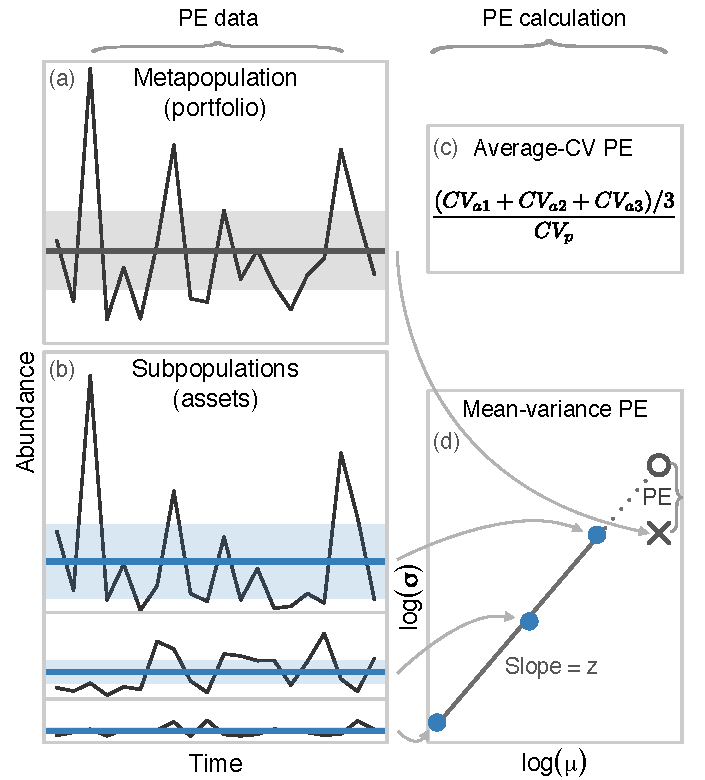
\includegraphics[height=4in]{prophets/fig1}
  \caption[Estimating the two PEs from empirical data.]{
  Estimating the two PEs from empirical data. (a, b) Example
    metapopulation (portfolio) and subpopulation (asset) abundance time-series.
    Horizontal lines represent the time-series' means and the shaded regions
    represent variability. (c) We calculated the average-CV PE by dividing the
    average CV of the subpopulations ($\CV_a$) by the CV of the metapopulation
    ($\CV_p$). (d) We calculated the mean-variance PE by (1) plotting the mean
    and variance of each subpopulation on log-log axes, (2) extrapolating the
    subpopulation mean-variance relationship to the metapopulation mean
    (open-grey circle), and (3) comparing the predicted (open-grey circle) and
    observed (grey cross) metapopulation variability. Both methods will
    estimate the same PE if the slope of the log-log plot (z) equals two.
  }
  \label{fig:didactic}
\end{figure}

\clearpage
\begin{figure}[htbp]
  \centering 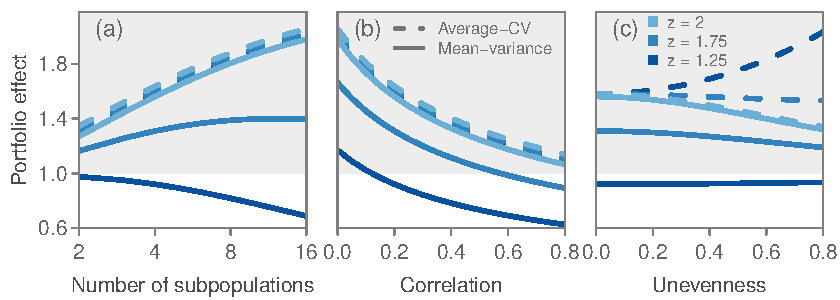
\includegraphics[width=4.8in]{prophets/fig2}
  \caption[The ecological factors driving the PE in theoretical systems.]{
  The ecological factors driving the PE in theoretical systems. A PE of
    two, for example, would indicate a two-fold increase in stability for the
    portfolio compared to what we would expect in a single homogeneous
    population of the same size. We show the mean-variance PE and average-CV PE
    for three z values across (a) number of subpopulations, (b)
    correlation between subpopulation time-series, and (c) unevenness of mean
    subpopulation abundance. We generated uneven mean subpopulation abundances
    by drawing four values at quantiles of 0.2, 0.4, 0.6, and 0.8
    from a log-normal distribution
    with log-mean $\mu$ ($\mu = 2$) and log-standard deviation of the
    unevenness value (the x-axis) times $\mu$. We fixed correlation at 0.2 and subpopulation
    number at four in all panels where these parameters weren't varying. The
    grey-shading indicates stabilizing PEs. Both PE definitions are equal
    across all scenarios at z = 2. In panels (a) and (b) the average-CV PE is
    the same regardless of z.
  } \label{fig:lines}
\end{figure}

%\bigskip
\clearpage
\begin{figure}[htbp]
  \centering 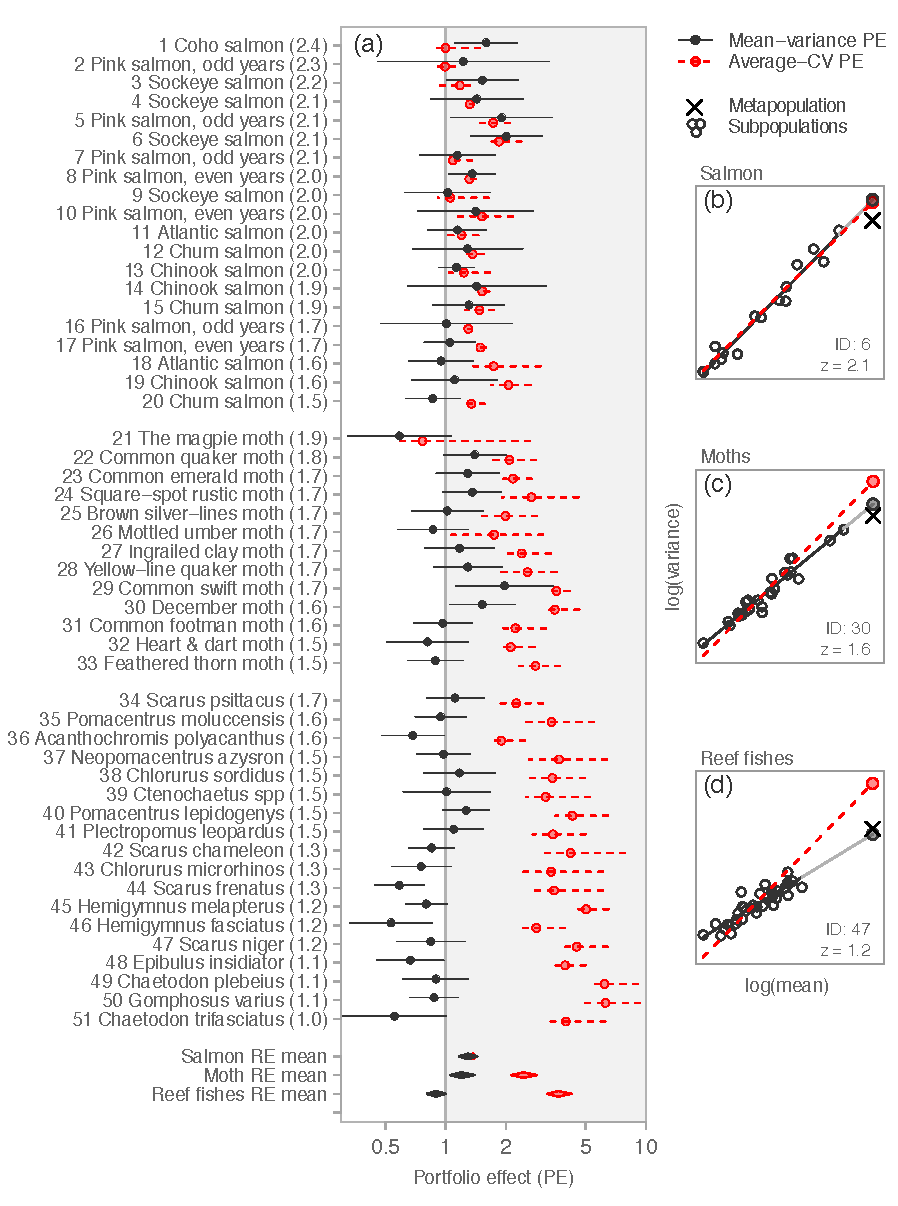
\includegraphics[height=5.5in]{prophets/fig3}
  \caption[PEs across 51 metapopulations.]{
  PEs across 51 metapopulations. (a) Empirical PEs (circles) and 95\%
    CIs (lines) for the mean-variance method and the average-CV PE method.
    We ordered metapopulations within taxonomic groups by Taylor's law z values
    (indicated in brackets beside each metapopulation name). Diamonds represent
    inverse-variance weighted random-effect (RE) meta-analytic means and 95\%
    CIs. Numbers before population names represent population IDs (see
    Supplementary Table 1). PEs $>$ 1 (grey shading) represent stabilizing
    effects; note the log-distributed x-axis. (b, c, d) Examples of using
    Taylor's power law to calculate the mean-variance PE. The solid black
    regression line projects the subpopulation mean-variance relationship to the
    metapopulation mean abundance (shaded grey circle). The $\times$ denotes the
    observed metapopulation mean and variance. The ratio of the observed to
    predicted variance represents the mean-variance PE. The red circle denotes
    the average-CV PE and the dashed-red line the mean-variance relationship
    under the assumption that z = 2, as the average-CV PE assumes.
  }
  \label{fig:meta}
\end{figure}
%
%\bigskip
\clearpage
\begin{figure}[htbp]
  \centering 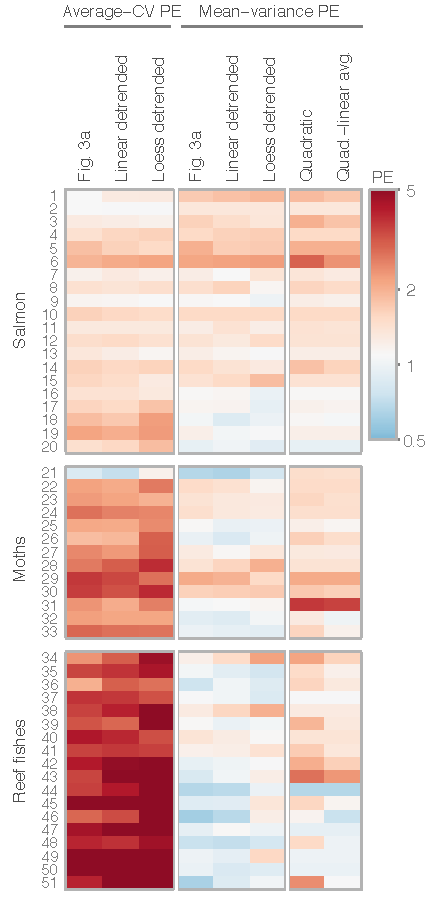
\includegraphics[height=5in]{prophets/fig4}
  \caption[The sensitivity of PE metrics across two detrending methods and three mean-variance model fits.]{
  The sensitivity of PE metrics across two detrending (linear and
    loess) methods (columns 2--3 and 5--6) and three mean-variance model fits
    (columns 4, 7--8). Columns 1 and 4 represent the same PEs as shown in
    Fig.~\ref{fig:meta}, but with colour indicating the strength of stabilizing
    effect. Red indicates a stabilizing PE, blue indicates a destabilizing PE,
    and white indicates a neutral PE. The y-axis shows the same metapopulation
    IDs as Fig.~\ref{fig:meta}.
  }
  \label{fig:detrend}
\end{figure}

%\bigskip
\clearpage
\begin{figure}[htbp]
  \centering
  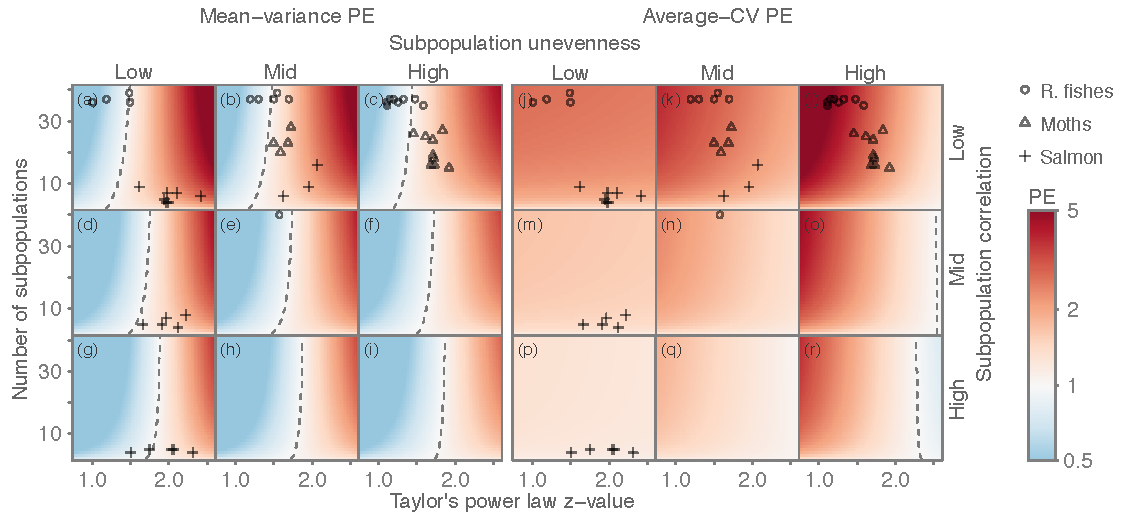
\includegraphics[width=\textwidth]{prophets/fig5}
  \caption[Empirical ecological PEs overlaid in theoretical PE
    parameter space.]{
  Empirical ecological PEs (points) overlaid in theoretical PE
    parameter space (colour shading). The colour shading indicates the
    stabilizing-effect of the theoretical mean-variance PEs (a--i) and
    average-CV PEs (j--r): red indicates a stabilizing effect and blue indicates
    a destabilizing effect.
    The dashed lines indicate neutral PEs. Columns from left to right
    show systems with increasingly uneven subpopulation sizes,
    and rows from top to bottom show systems with increasingly strong mean
    correlation between subpopulation (see the Supporting
    Information).
  } \label{fig:paramspace}
\end{figure}

%\bigskip
\clearpage
\begin{figure}[htbp]
  \centering 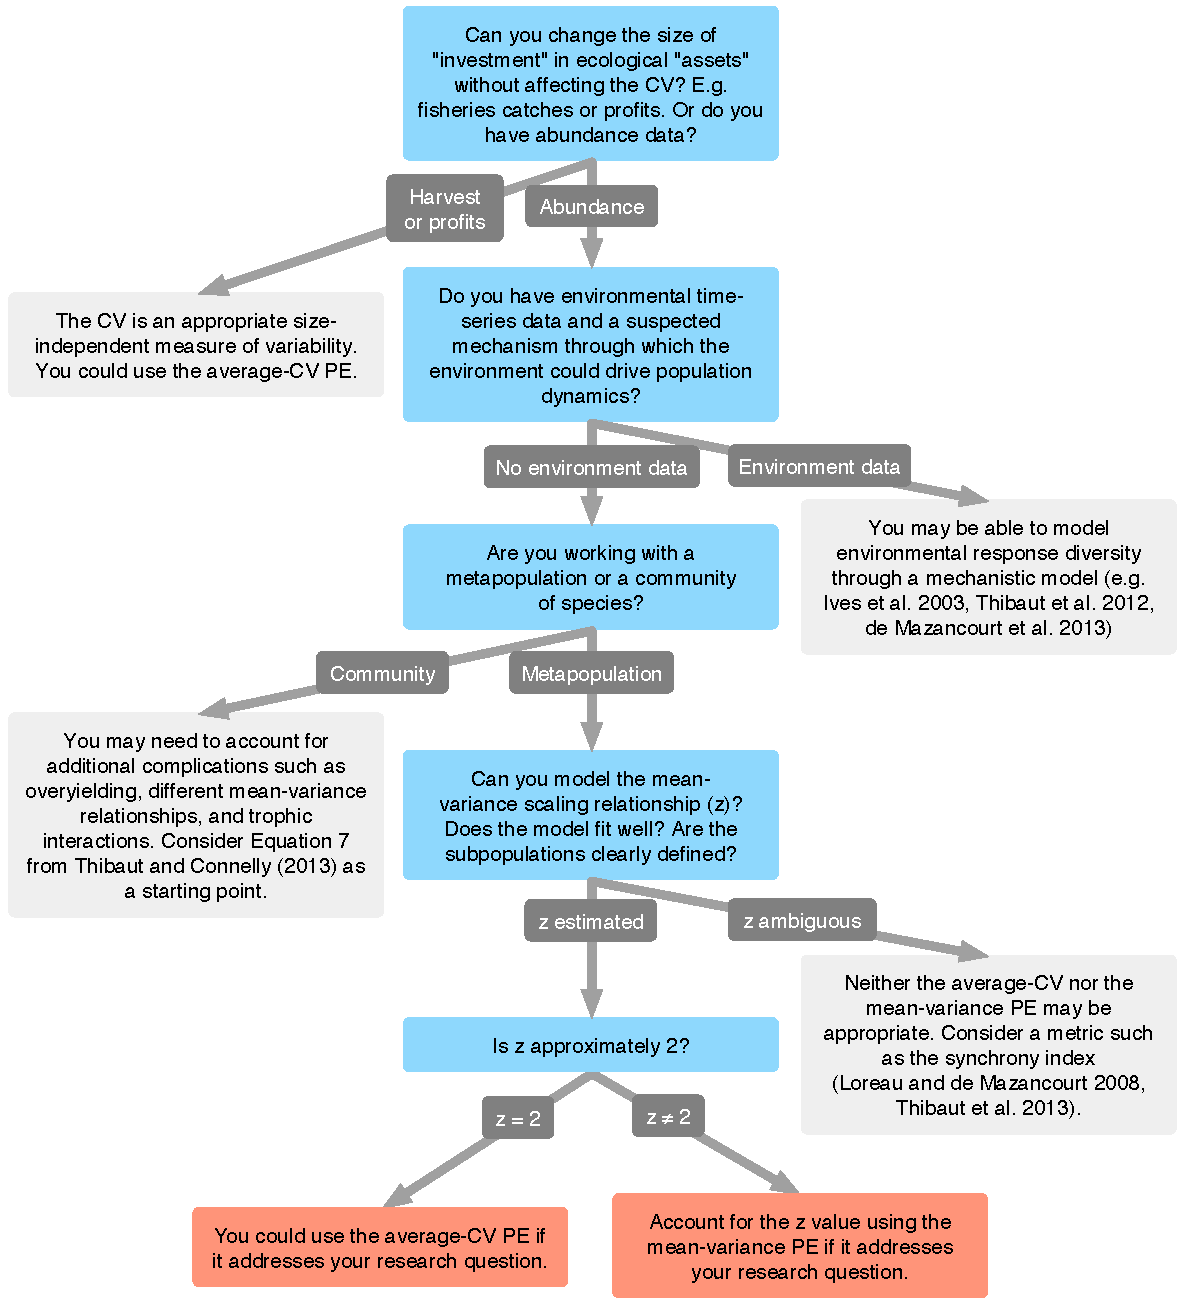
\includegraphics[width=5.2in]{prophets/fig6}
  \caption[Decision tree showing options for quantifying ecological portfolios.]{
  %\noindent
  %\textbf{Fig.\ 6.}
  Decision tree showing options for quantifying ecological portfolios.
    Blue boxes in the middle column show questions to ask of the study system
    and available data.
    The orange boxes at the bottom represent the methods demonstrated in
    this paper. The light-grey boxes along the sides show other options to
    quantify ecological portfolios given different research questions, study
    systems, and available data.
  } \label{fig:recommendations}
\end{figure}
%
%    %\end{spacing}
%    \end{document}

\begin{appendices}
\section{Supporting materials}

\subsection{R package to estimate metapopulation portfolio effects}

%In an R console, the ecofolio package can be installed either
%from the included source package (\texttt{.tar.gz} file)
%, from the Mac or
%Windows binary packages (\texttt{.tgz} or \texttt{.zip}, respectively)
%or via the web (instructions below). First, install dependencies if needed:

% \begin{verbatim}
% install.packages(c("plyr", "reshape", "MuMIn", "robustbase"))
% \end{verbatim}
%
% \noindent
% Then, to install the included package:
%
% %install.packages("ecofolio_0.1.tar.gz", type = "source")
%
% \begin{verbatim}
% install.packages("mee312093-sup-0001-Sourcepackage.tar.gz", type = "source")
% \end{verbatim}

%install.packages("ecofolio_0.1.tgz") # Mac binary
%install.packages("ecofolio_0.1.zip") # Windows binary

%\noindent
In an R console, the ecofolio package can be installed with,

\begin{verbatim}
# install.packages("devtools") # if needed
devtools::install_github("seananderson/ecofolio")
\end{verbatim}

\noindent
Current code and install details are available at\\ \url{https://github.com/seananderson/ecofolio}
%\clearpage

%Install details are available at:
%\url{https://github.com/seananderson/ecofolio}

\noindent
You can load the package, read the vignette, and access the help pages with:

\begin{verbatim}
library("ecofolio")
vignette("ecofolio")
help(package = "ecofolio")
\end{verbatim}

\subsection{Data sources for the empirical portfolio effect analysis}
We sought to include as many metapopulation time series from as diverse
taxonomic groups as possible. However, due to availability, the included data
primarily represent metapopulations in North America (salmon), the United
Kingdom (moths), and Australia (reef fishes) (Figure~\ref{fig:map}). We show a
summary of the data included in our analysis of empirical ecological systems
in Table~\ref{tab:datasources} and the time series in Figure~\ref{fig:ts}.

\subsubsection{Salmon}
We obtained salmon data from a variety of sources, in particular
\citet{dorner2008}. Most of the salmon populations are from the northwest
coast of North America, but also: Kola Peninsula, Russia
\citep{jensen1999}, southern New England \citep{kocik2006}, and
Central Valley, California \citep{carlson2011} (Figure~\ref{fig:map}). All
data represent annual estimated returns---fisheries catch plus escapement to
the spawning grounds. We divided pink salmon annual estimated returns into odd-
and even-year time series due to their strongly distinct runs that do not
interbreed \citep{quinn2005}. To maintain consistency with previous PE
analyses involving sockeye salmon \citep{schindler2010} and analyses of
time series of these data \citep{dorner2008}, and due to the less distinct
separate runs \citep{quinn2005}, we did not divide the sockeye salmon into
separate runs.

Subsets of these salmon data have been used in numerous analyses relating
diversity with stability. A particular feature of the salmon literature is a
focus on the role of ``biocomplexity''---a diversity of life-histories and
local adaptations to the environment---in producing stability
\citep{hilborn2003} and recent papers have focussed on measuring the
portfolio effects we investigate in this paper \citep{schindler2010,
  carlson2011}. In studying the mechanisms behind subpopulation
asynchrony, and hence portfolio effects, studies of Pacific salmon have
generally focussed on drivers that fall into two categories: (1) landscape
filtering of the environment so that different subpopulations experience
different environmental forces (e.g.\ local topology affecting stream flow)
\citep[e.g.][]{schindler2008}, and (2) biologically-based response
diversity to the environment (e.g.\ genetically-based variation in thermal
tolerances) \citep[e.g.][]{eliason2011}. These patterns of asynchrony can
play out not just at the decadal scale but also over centuries
\citep{rogers2013}.

\subsubsection{Moths}
We obtained moth abundance time series from the Rothamsted Insect Survey
(RIS). L. R. Taylor started the trap network that forms the RIS in the early
1960s; the RIS is now one of the longest-running and largest-scale insect
surveys in the world \citep{conrad2004}. Details on the survey are
available in \citet{conrad2004} and \citet{taylor1986}. The RIS
captures moths by light traps \citep{williams1948} placed 1--2 m above
ground; these traps catch small but reliable samples of moth populations
\citep{williams1948, taylor1974, conrad2004}. Although
different species may show different responses to the traps
\citep{muirhead-thomson1991, woiwod1992}, we compare across sites
within the same species so this should not affect our results.

Our moth data spanned from 1999--2010 for 13 species (Table~\ref{tab:datasources}) and 28 sites
(Table~\ref{tab:ris-meta}). We included only moths with single broods per year
(univoltine moths) and single annual flight episodes since we were aggregating
the data annually to maintain consistency with data from other taxonomic
groups that were available. We removed site-species combinations where there
were eight or more years with zero moths caught in traps to avoid sites where
a given species was exceptionally rare and not likely to be consistently
censused. This removed 97 subpopulations leaving 280. Further culling of
populations according to the criteria in the Methods section left us with 268
subpopulations. All the species included are common within Great Britain,
although some have undergone declines in abundance since the RIS began
\citep{conrad2004}.

Earlier versions of these moth data featured heavily in the work of
Taylor and colleagues on the property now known as Taylor's power law
\citep{taylor1977, taylor1980, perry1981}. This early work
focussed on behavioural properties that might regulate the stability and
variance of moth populations \citep{taylor1980}. Work has continued with
these datasets and studies have shown a number of mechanisms generating
stability. For example, authors have shown spatial asynchrony
\citep{gaston1988}, polyphagy (eating different kinds of food)
\citep{redfearn1988}, and density dependence to act as stabilizing forces
\citep{hanski1993}.

\subsubsection{Reef fishes}

We obtained reef visual census fish counts within the Greater Barrier Reef
(GBR) from the Australian Institute of Marine Science's (AIMS) Long-term
Monitoring Program (LTMP) \citep{sweatman2008}. The AIMS survey data used
here are from fixed transects at selected sites across 46 reefs from
1994--2010 (Table~\ref{tab:grb-meta}). Details of the sampling design are
available from \citet{halford1994}. Briefly, AIMS surveys reef fish
annually within six sectors of the GBR. AIMS identifies inner-, \mbox{mid-,}
and outer-shelf positions and three reefs within each shelf position. Within
each reef, AIMS chooses three sites of the same habitat and establishes five
permanent 50m transects at 6--9m depth 10m apart and parallel to the reef
crest. Divers count damselfishes (Pomacentrids) on 1m-wide transects and all
other families on 5m-wide transects. AIMS only censuses fish one year or older
since recruitment can be highly spatially and temporally variable. AIMS
conducts annual standardization exercises to avoid temporal bias in counts
within and across divers \citep{halford1994}.

A number of recent studies have used these reef-fish data to
investigate stability-diversity relationships, often focusing on functional
diversity or reef size and isolation. For example, \citet{thibaut2012}
found strong asynchrony of response to the environment between three functional
groups of herbivorous reef fishes, which lead to greater stability. Another
benefit to this functional diversity may be increased disease resistance
\citep{raymundo2009}, presumably enhancing stability. Independent of
functional roles, \citet{mellin2010} found that small, isolated reefs have
higher population variability and therefore higher probability of local
extinction.

\subsection{Diagnosing the ecological properties of empirical portfolio effects}

We overlaid the empirical PEs in their respective theoretical parameter space
to investigate the ecological properties of real-world metapopulations
(subpopulation correlation, mean-variance scaling, subpopulation number
richness, and evenness). Specifically, we matched the empirical
linear-regression z values and the number of subpopulations with their
theoretical counterparts.

To present our results graphically in Figure~\ref{fig:paramspace}, we categorized
the mean correlation of the empirical subpopulations ($\bar{\rho}$) into bins of
$0 \le \bar{\rho} < 0.25$, $0.25 \le \bar{\rho} < 0.5$, and $0.50 \le \bar{\rho}
< 75$ and matched these with the theoretical PE estimated at the midpoints of
these bins (i.e.\ 0.125, 0.375, and 0.625).  We matched the disparity in
subpopulation size by: (1) calculating the CV of the log of the subpopulation
time series' means, $\CV(\log\mu)$; (2) categorizing the empirical
metapopulations into bins of $0 \le \CV(\log\mu) < 0.3$, $0.3 \le \CV(\log\mu) <
0.6$, and $0.6 \le \CV(\log\mu) < 0.9$; (3) estimating the theoretical PE using
evenly-spaced values from a log-normal distribution with a mean of two and
standard deviation of the midpoints of these bins (i.e.\ 0.15, 0.45, and 0.75).
Here and in Figure~\ref{fig:lines}, we derived these evenly-spaced values as
follows.
We drew subpopulation ($i$) quantiles $q_i$ from the evenly-spaced sequence:
$a_1, a_2, \ldots, a_n$, where $a_1 = 1/(n+1)$ and $a_n = 1-(1/(n+1))$. We then
calculated the subpopulation means at each $q_i$ from a log-normal distribution
with log-mean of two and a log-standard deviation of the ``unevenness value''
times the log-mean.

% \renewcommand{\baselinestretch}{\tighttextstretch} %% get smaller spacing
% \normalsize
% \bibliographystyle{apalike}
% \bibliography{/Users/seananderson/Dropbox/tex/jshort,/Users/seananderson/Dropbox/tex/ref3}
% \clearpage
% \renewcommand{\baselinestretch}{\textstretch} %% get normal spacing
% \normalsize

%\renewcommand{\thetable}{A\arabic{table}}
%\setcounter{table}{0}

%\renewcommand{\thefigure}{A\arabic{figure}}
%\renewcommand{\figurename}{Figure}
%\setcounter{figure}{0}

\subsection{Supporting Tables and Figures}

\begin{landscape}


  % latex table generated in R 2.15.0 by xtable 1.7-0 package
% Tue Sep 18 15:07:29 2012
\begin{table}[ht]
\begin{center}
\caption{Metapopulations used in the empirical PE analyses. ID column numbers correspond to ID numbers in the figures.}
\label{tab:datasources}
{\tiny
\begin{tabular}{rlllrrl}
  \toprule
ID & Species & Common & Location & Subpopulations & Years & Reference \\ 
  \midrule
  1 & \textit{Oncorhynchus kisutch} & Coho salmon & Broughton archipelago, BC, Canada &   6 &  16 & \citep{krkosek2011} \\ 
    2 & \textit{Oncorhynchus gorbuscha} & Pink salmon, odd years & Puget Sound, WA, United States &   4 &  19 & \citep{dorner2008} \\ 
    3 & \textit{Oncorhynchus nerka} & Sockeye salmon & Bristol Bay, AK, United States &   8 &  43 & \citep{west2006} \\ 
    4 & \textit{Oncorhynchus nerka} & Sockeye salmon & Kodiak, AK, United States &   4 &  24 & \citep{dorner2008} \\ 
    5 & \textit{Oncorhynchus gorbuscha} & Pink salmon, odd years & Broughton archipelago, BC, Canada &   7 &  19 & \citep{krkosek2011} \\ 
    6 & \textit{Oncorhynchus nerka} & Sockeye salmon & Fraser River, BC, Canada &  16 &  44 & \citep{dorner2008} \\ 
    7 & \textit{Oncorhynchus gorbuscha} & Pink salmon, odd years & Kodiak, AK, United States &   5 &   8 & \citep{dorner2008} \\ 
    8 & \textit{Oncorhynchus gorbuscha} & Pink salmon, even years & Chignik, AK, United States &   5 &  16 & \citep{dorner2008} \\ 
    9 & \textit{Oncorhynchus nerka} & Sockeye salmon & Upper Cook Inlet, AK, United States &   4 &  29 & \citep{fair2011} \\ 
   10 & \textit{Oncorhynchus gorbuscha} & Pink salmon, even years & Broughton archipelago, BC, Canada &   7 &  19 & \citep{krkosek2011} \\ 
   11 & \textit{Salmo salar} & Atlantic salmon & Kola Peninsula, Russia &   4 &  15 & \citep{jensen1999} \\ 
   12 & \textit{Oncorhynchus keta} & Chum salmon & Puget Sound, WA, United States &   7 &  26 & \citep{dorner2008} \\ 
   13 & \textit{Oncorhynchus tshawytscha} & Chinook salmon & Columbia Estuary, OR/WA, United States &   9 &  23 & \citep{streamnet2011} \\ 
   14 & \textit{Oncorhynchus tshawytscha} & Chinook salmon & Elochoman River, WA, United States &   5 &  27 & \citep{streamnet2011} \\ 
   15 & \textit{Oncorhynchus keta} & Chum salmon & Arctic, Yukon, Kuskokwim, US and Canada &   5 &  18 & \citep{dorner2008} \\ 
   16 & \textit{Oncorhynchus gorbuscha} & Pink salmon, odd years & Chignik, AK, United States &   5 &  15 & \citep{dorner2008} \\ 
   17 & \textit{Oncorhynchus gorbuscha} & Pink salmon, even years & Kodiak, AK, United States &   5 &   9 & \citep{dorner2008} \\ 
   18 & \textit{Salmo salar} & Atlantic salmon & Southern New England, United States &   6 &  39 & \citep{kocik2006} \\ 
   19 & \textit{Oncorhynchus tshawytscha} & Chinook salmon & Central Valley, California &   9 &  54 & \citep{carlson2011} \\ 
   20 & \textit{Oncorhynchus keta} & Chum salmon & Alaska Peninsula, AK, United States &   4 &  32 & \citep{dorner2008} \\ 
   21 & \textit{Abraxas grossulariata} & The magpie moth & UK &  15 &  12 & \citep{conrad2004} \\ 
   22 & \textit{Orthosia cerasi} & Common quaker moth & UK &  27 &  12 & \citep{conrad2004} \\ 
   23 & \textit{Hemithea aestivaria} & Common emerald moth & UK &  16 &  12 & \citep{conrad2004} \\ 
   24 & \textit{Xestia xanthographa} & Square-spot rustic moth & UK &  28 &  12 & \citep{conrad2004} \\ 
   25 & \textit{Petrophora chlorosata} & Brown silver-lines moth & UK &  18 &  12 & \citep{conrad2004} \\ 
   26 & \textit{Erannis defoliaria} & Mottled umber moth & UK &  19 &  12 & \citep{conrad2004} \\ 
   27 & \textit{Diarsia mendica} & Ingrailed clay moth & UK &  24 &  12 & \citep{conrad2004} \\ 
   28 & \textit{Agrochola (Leptologia) macilenta} & Yellow-line quaker moth & UK &  23 &  12 & \citep{conrad2004} \\ 
   29 & \textit{Pharmacis lupulina} & Common swift moth & UK &  16 &  12 & \citep{conrad2004} \\ 
   30 & \textit{Poecilocampa populi} & December moth & UK &  25 &  12 & \citep{conrad2004} \\ 
   31 & \textit{Eilema lurideola} & Common footman moth & UK &  20 &  12 & \citep{conrad2004} \\ 
   32 & \textit{Agrotis exclamationis} & Heart and dart moth & UK &  23 &  12 & \citep{conrad2004} \\ 
   33 & \textit{Colotois pennaria} & Feathered thorn moth & UK &  26 &  12 & \citep{conrad2004} \\ 
   34 & \textit{Scarus psittacus} & \textit{Scarus psittacus} & GBR, Australia &  37 &  14 & \citep{sweatman2008} \\ 
   35 & \textit{Pomacentrus moluccensis} & \textit{Pomacentrus moluccensis} & GBR, Australia &  35 &  14 & \citep{sweatman2008} \\ 
   36 & \textit{Acanthochromis polyacanthus} & \textit{Acanthochromis polyacanthus} & GBR, Australia &  40 &  14 & \citep{sweatman2008} \\ 
   37 & \textit{Neopomacentrus azysron} & \textit{Neopomacentrus azysron} & GBR, Australia &  39 &  14 & \citep{sweatman2008} \\ 
   38 & \textit{Chlorurus sordidus} & \textit{Chlorurus sordidus} & GBR, Australia &  37 &  14 & \citep{sweatman2008} \\ 
   39 & \textit{Ctenochaetus spp} & \textit{Ctenochaetus spp} & GBR, Australia &  36 &  14 & \citep{sweatman2008} \\ 
   40 & \textit{Pomacentrus lepidogenys} & \textit{Pomacentrus lepidogenys} & GBR, Australia &  39 &  14 & \citep{sweatman2008} \\ 
   41 & \textit{Plectropomus leopardus} & \textit{Plectropomus leopardus} & GBR, Australia &  37 &  14 & \citep{sweatman2008} \\ 
   42 & \textit{Scarus chameleon} & \textit{Scarus chameleon} & GBR, Australia &  37 &  14 & \citep{sweatman2008} \\ 
   43 & \textit{Chlorurus microrhinos} & \textit{Chlorurus microrhinos} & GBR, Australia &  37 &  14 & \citep{sweatman2008} \\ 
   44 & \textit{Scarus frenatus} & \textit{Scarus frenatus} & GBR, Australia &  36 &  14 & \citep{sweatman2008} \\ 
   45 & \textit{Hemigymnus melapterus} & \textit{Hemigymnus melapterus} & GBR, Australia &  37 &  14 & \citep{sweatman2008} \\ 
   46 & \textit{Hemigymnus fasciatus} & \textit{Hemigymnus fasciatus} & GBR, Australia &  37 &  14 & \citep{sweatman2008} \\ 
   47 & \textit{Scarus niger} & \textit{Scarus niger} & GBR, Australia &  37 &  14 & \citep{sweatman2008} \\ 
   48 & \textit{Epibulus insidiator} & \textit{Epibulus insidiator} & GBR, Australia &  37 &  14 & \citep{sweatman2008} \\ 
   49 & \textit{Chaetodon plebeius} & \textit{Chaetodon plebeius} & GBR, Australia &  35 &  14 & \citep{sweatman2008} \\ 
   50 & \textit{Gomphosus varius} & \textit{Gomphosus varius} & GBR, Australia &  36 &  14 & \citep{sweatman2008} \\ 
   51 & \textit{Chaetodon trifasciatus} & \textit{Chaetodon trifasciatus} & GBR, Australia &  36 &  14 & \citep{sweatman2008} \\ 
   \bottomrule
\end{tabular}
}
\end{center}
\end{table}

\end{landscape}
\clearpage

% latex table generated in R 2.15.0 by xtable 1.7-0 package
% Tue Sep 18 15:07:31 2012
\begin{table}[ht]
\begin{center}
\caption{Moth sites used from the Rothamsted Insect Survey database. Sites are ordered from north to south. County refers to the British County. ``Number of spp.''\ refers to the number of moth species remaining that matched our inclusion criteria.}
\label{tab:ris-meta}
{\footnotesize
\begin{tabular}{llrrrr}
  \toprule
Site name & County & Northing & Easting & Altitude (m) & Number of spp. \\ 
  \midrule
Starcross & South Devon & 821 & 2972 & 9 & 12 \\ 
  Denny Lodge & South Hampshire & 1056 & 4333 & 30 & 10 \\ 
  Bentley Wood & South Wiltshire & 1324 & 4253 & 130 & 12 \\ 
  Winkworth & Surrey & 1412 & 4991 & 130 & 12 \\ 
  Alice Holt & North Hampshire & 1428 & 4803 & 122 & 12 \\ 
  Perry Wood & East Kent & 1565 & 6040 & 80 & 13 \\ 
  Wisley II & Surrey & 1579 & 5065 & 40 & 10 \\ 
  Westonbirt & West Gloucestershire & 1898 & 3847 & 46 & 13 \\ 
  Geescroft I & Hertfordshire & 2128 & 5132 & 130 & 12 \\ 
  Allotments & Hertfordshire & 2134 & 5134 & 130 & 7 \\ 
  Barnfield & Hertfordshire & 2135 & 5132 & 130 & 10 \\ 
  Hereford & Herefordshire & 2476 & 3564 & 91 & 10 \\ 
  Cockayne Hatley & Bedfordshire & 2494 & 5253 & 76 & 11 \\ 
  Llysdinam & Breconshire  & 2586 & 3009 & 197 & 11 \\ 
  Tregaron & Cardiganshire & 2618 & 2687 & 198 & 10 \\ 
  Broom's Barn & West Suffolk & 2656 & 5752 & 73 & 9 \\ 
  Compton Park & Staffordshire & 2988 & 3889 & 105 & 9 \\ 
  Preston Montford II & Shropshire & 3143 & 3433 & 61 & 13 \\ 
  Malham Tarn & Mid-west Yorkshire & 4672 & 3894 & 396 & 8 \\ 
  Shildon & County Durham & 5262 & 4239 & 150 & 9 \\ 
  Forest-in-Teesdale & North-west Yorkshire & 5306 & 3853 & 381 & 5 \\ 
  Castle Eden Dene l & County Durham & 5394 & 4428 & 91 & 10 \\ 
  Auchincruive II & Ayrshire & 6233 & 2377 & 52 & 10 \\ 
  Brodick & Clyde Islands & 6380 & 2014 & 50 & 8 \\ 
  Rowardennan & Stirlingshire & 6960 & 2378 & 15 & 8 \\ 
  Kindrogan & East Perthshire & 7630 & 3055 & 259 & 7 \\ 
  Beinn Eighe I & West Ross \& Cromarty & 8629 & 2024 & 25 & 9 \\ 
  Cromarty & East Ross \& Cromarty & 8672 & 2785 & 30 & 10 \\ 
   \bottomrule
\end{tabular}
}
\end{center}
\end{table}

\clearpage
% latex table generated in R 2.15.0 by xtable 1.7-0 package
% Tue Sep 18 15:07:33 2012
\begin{table}[ht]
\begin{center}
\caption[Reef locations used from the AIMS LTMP Great Barrier Reef database.]{Reef locations used from the AIMS LTMP Great Barrier Reef database.
  Reefs are ordered from north to south. ``Number of spp.''\ refers to the
  number of fish species remaining that matched our inclusion criteria.}
\label{tab:grb-meta}
{\footnotesize
\begin{tabular}{lrrr}
  \toprule
Reef & Latitude (deg south) & Longitude (deg east) & Number of spp. \\
  \midrule
Carter Reef & 14.52 & 145.58 & 17 \\
  Yonge Reef & 14.57 & 145.62 & 16 \\
  No Name Reef & 14.62 & 145.64 & 18 \\
  Macgillivray Reef & 14.64 & 145.49 & 18 \\
  Lizard Island & 14.69 & 145.46 & 18 \\
  North Direction Reef & 14.74 & 145.51 & 18 \\
  Martin Reef(14123) & 14.75 & 145.37 & 18 \\
  Linnet Reef & 14.79 & 145.35 & 18 \\
  Agincourt Reefs (no 1) & 16.04 & 145.87 & 17 \\
  St Crispin Reef & 16.07 & 145.84 & 18 \\
  Opal (2) & 16.20 & 145.90 & 18 \\
  Low Islands Reef & 16.38 & 145.57 & 17 \\
  Hastings Reef & 16.49 & 146.02 & 17 \\
  Michaelmas Reef & 16.55 & 146.05 & 18 \\
  Green Island Reef & 16.77 & 145.97 & 18 \\
  Fitzroy Island Reef & 16.92 & 145.99 & 18 \\
  Myrmidon Reef & 18.25 & 147.38 & 18 \\
  Dip Reef & 18.39 & 147.45 & 17 \\
  Rib Reef & 18.47 & 146.88 & 18 \\
  John Brewer Reef & 18.62 & 147.08 & 18 \\
  Chicken Reef & 18.66 & 147.72 & 18 \\
  Davies Reef & 18.80 & 147.66 & 18 \\
  Pandora Reef & 18.81 & 146.43 & 3 \\
  Slate Reef & 19.66 & 149.91 & 18 \\
  Hyde Reef & 19.73 & 150.09 & 18 \\
  19131s & 19.77 & 149.38 & 18 \\
  Rebe Reef & 19.80 & 150.16 & 18 \\
  19138s & 19.80 & 149.43 & 18 \\
  Hayman Island Reef & 20.05 & 148.89 & 4 \\
  Langford-bird Reef & 20.07 & 148.87 & 4 \\
  Border Island Reef (no 1) & 20.18 & 149.03 & 13 \\
  East Cay Reef & 21.46 & 152.56 & 18 \\
  Turner Reef & 21.70 & 152.56 & 18 \\
  21529s & 21.87 & 152.18 & 18 \\
  Gannett Cay Reef & 21.98 & 152.47 & 18 \\
  Horseshoe & 22.02 & 152.62 & 18 \\
  Snake (22088) & 22.02 & 152.19 & 18 \\
  Broomfield Reef & 23.24 & 151.94 & 18 \\
  One Tree Reef & 23.48 & 152.09 & 18 \\
  Lady Musgrave Reef & 23.88 & 152.42 & 18 \\
   \bottomrule
\end{tabular}
}
\end{center}
\end{table}

\clearpage

\begin{figure}[htbp] \centering

  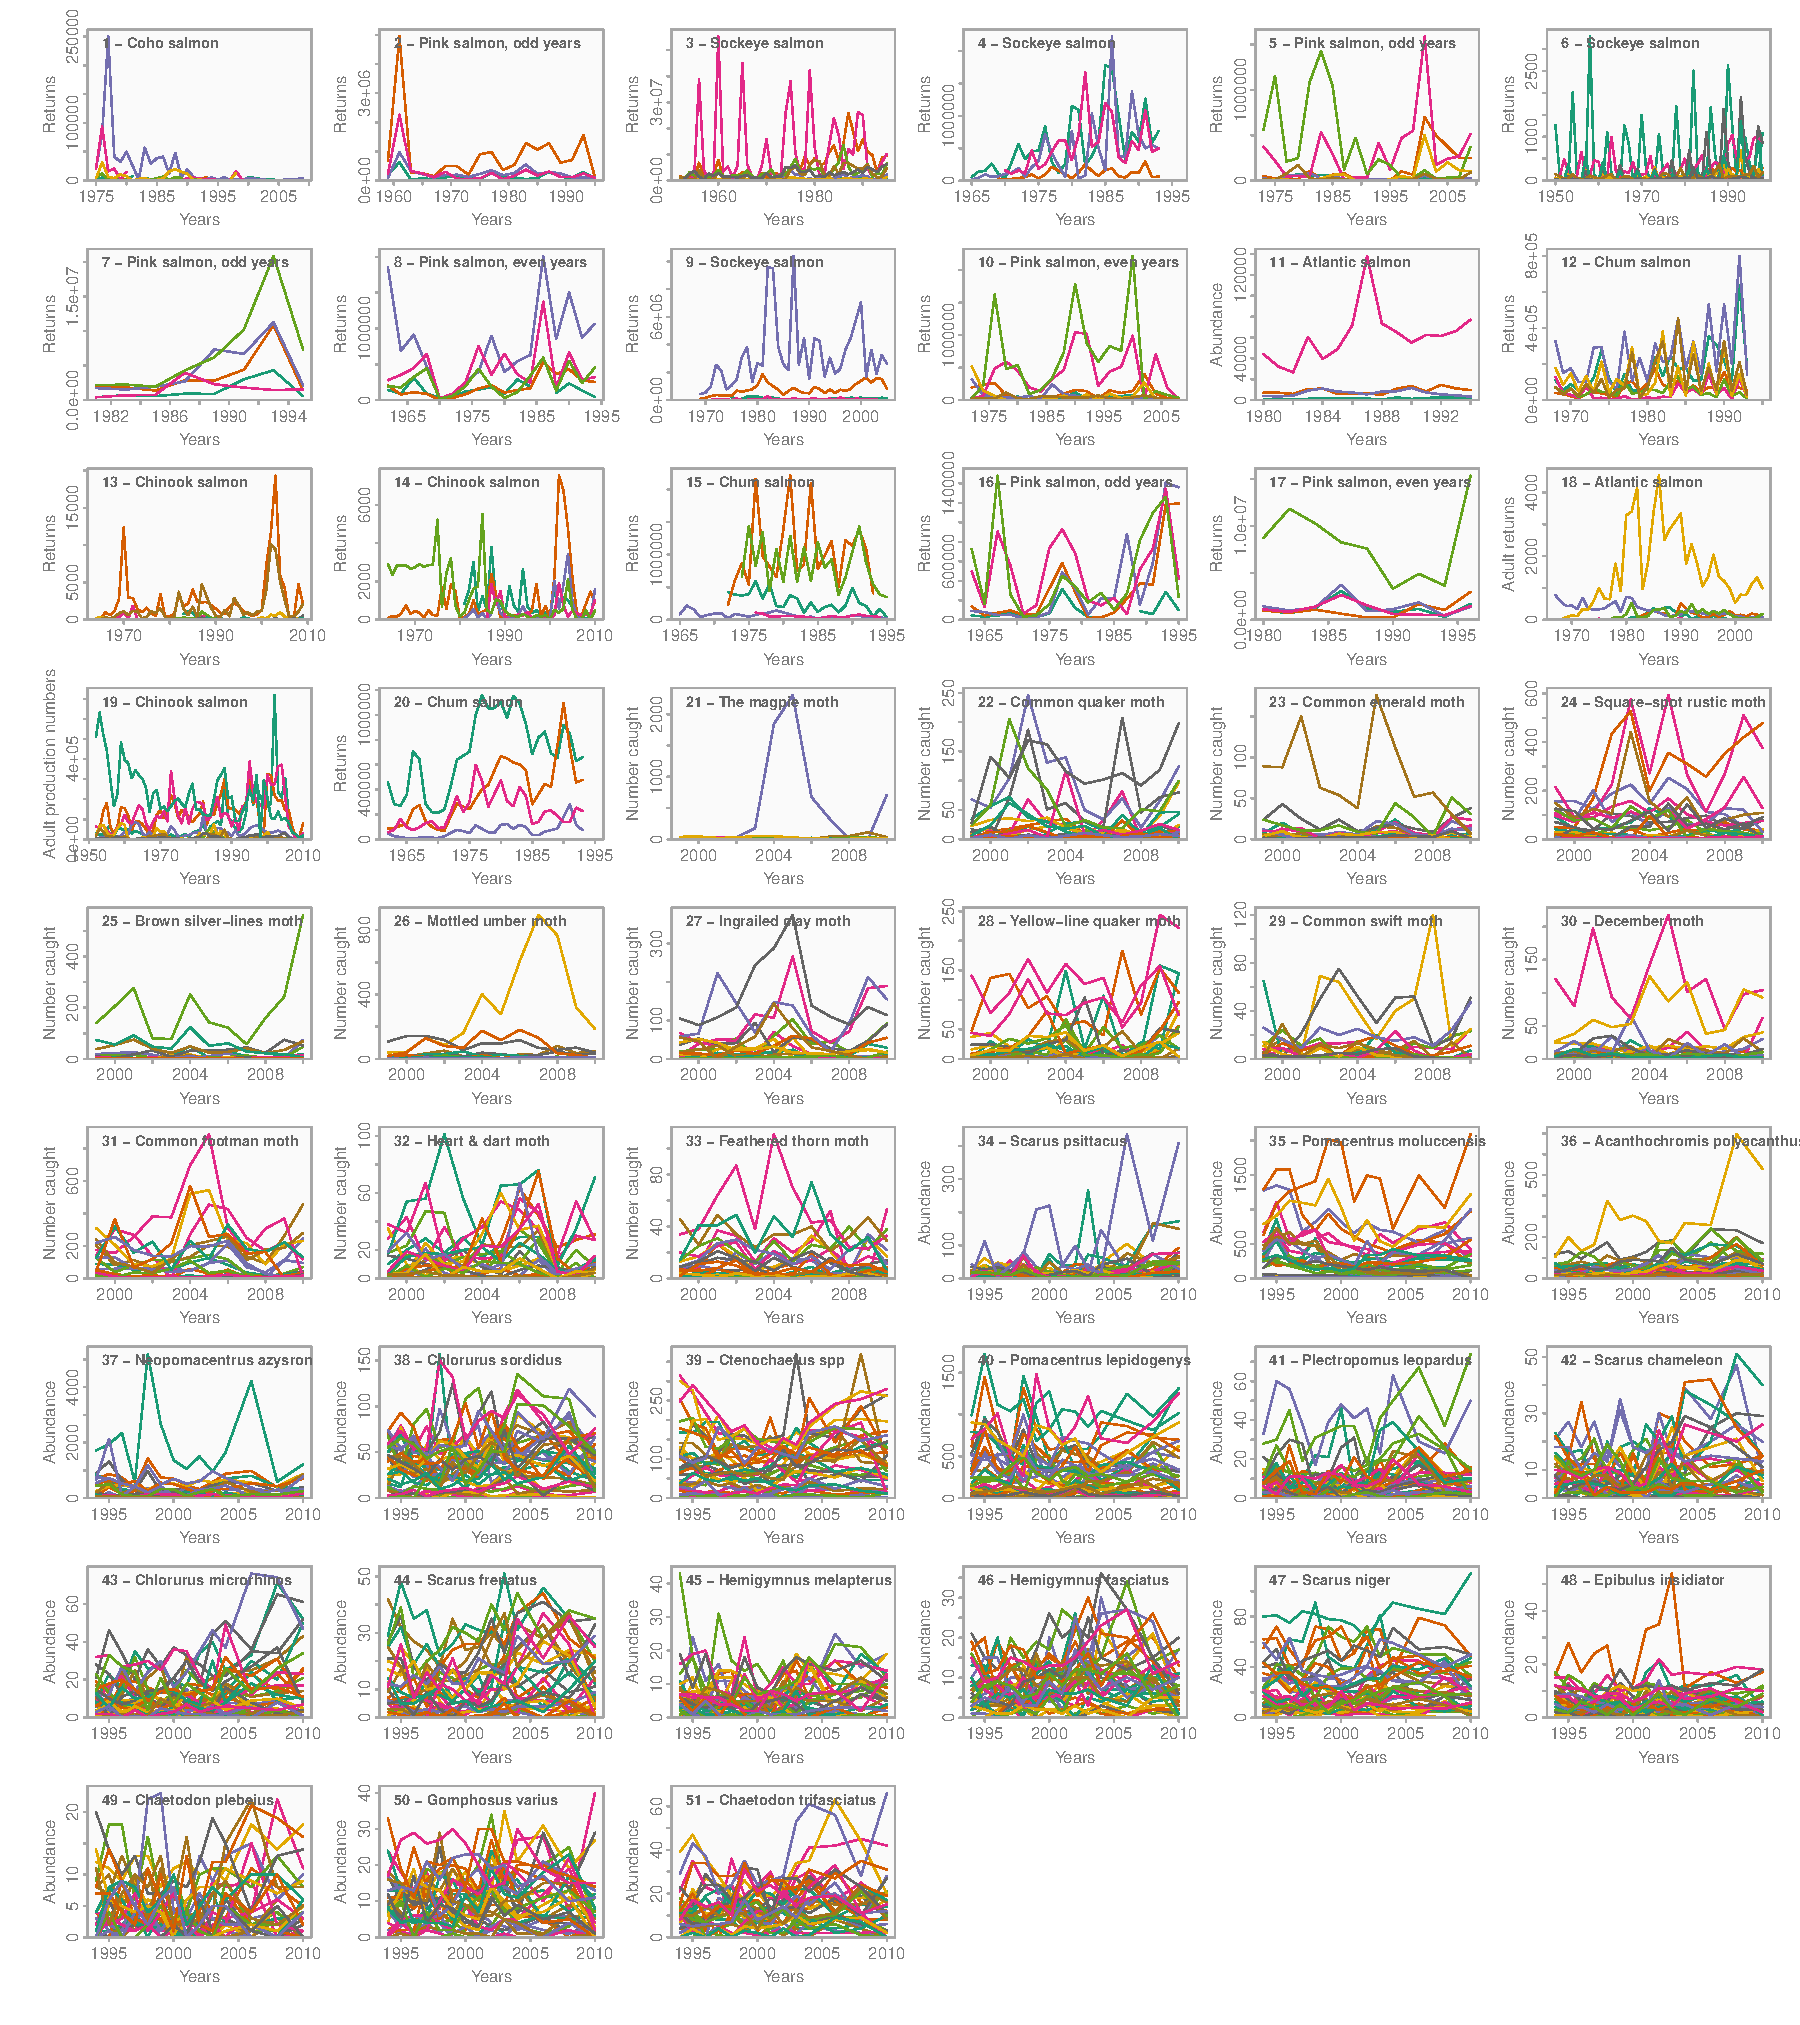
\includegraphics[width=\textwidth]{prophets/PE_data_series_ms.pdf}
  \caption[Subpopulation time series]{
    Subpopulation time series. Each panel contains one metapopulation.
    Colours were randomly assigned to distinguish subpopulations.
    Numbers in top-left corners refer to metapopulation IDs (see Table~\ref{tab:datasources}).
  } \label{fig:ts}
\end{figure}

\clearpage

\begin{figure}[htbp]
  \centering 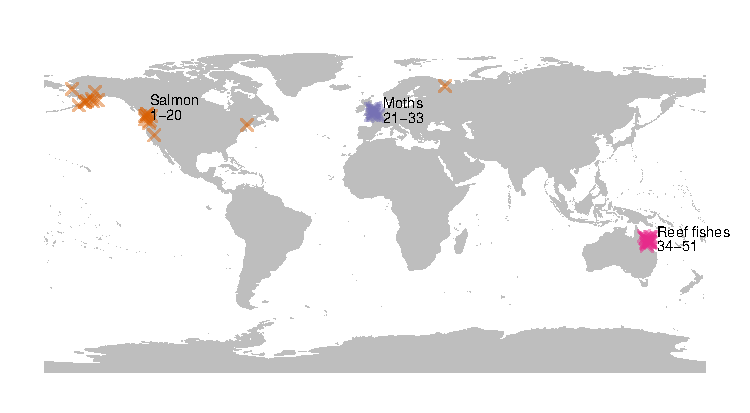
\includegraphics[width=5.5in]{prophets/PE_map_20120718.pdf}
  \caption[Map of included metapopulation]{
    Map of included metapopulations.  We represented salmon metapopulations
    with orange symbols, moths with purple, and reef fishes with pink.
    Numbers refer to metapopulation IDs (Table~\ref{tab:datasources}).  Points are jittered
    slightly for visual clarity.
  }
  \label{fig:map}
\end{figure}

\begin{figure}[htbp]
  \centering
  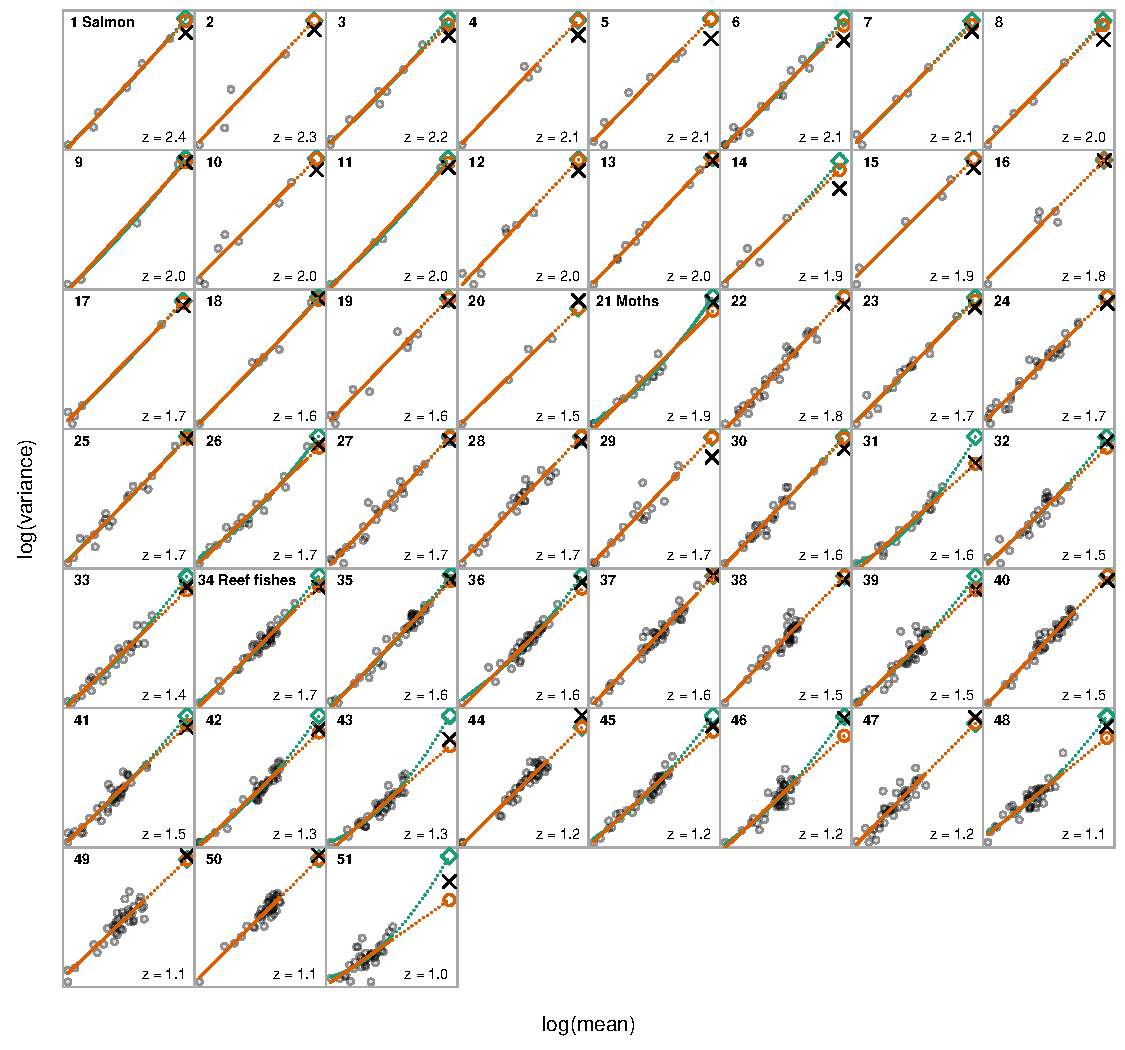
\includegraphics[width=\textwidth]{prophets/taylor-fits-scatter-20120720.pdf}
  \caption[Calculation of the \tilmanPE\ using Taylor's power law.]{Calculation of the \tilmanPE\ using Taylor's power law. Each
    dark-grey circle  represents the log($\mu$) and log($\sigma^2$) of an
    individual subpopulation timeseries.  The orange lines represent fitted
    linear regressions.  The green lines represent fitted quadratic
    regressions.  Black \texttt{x} symbols represent the observed
    metapopulation or portfolio mean and variance.  Dashed lines indicate the
    extrapolation of the model fit to the observed metapopulation or portfolio
    mean and variance.  Open-orange circles represent the predicted variance
    under the linear-fit assumption.  Open-green diamonds represent the
    predicted variance under the quadratic-fit assumption.  Metapopulations in
    which the predicted variance is greater than the observed variance
    represent variance-reducing PEs.  We ordered the panels by decreasing
    Taylor's power law \zvalue\ (slope of the linear regression) within
    taxonomic groupings.  Numbers in upper left of panels refer to
    metapopulation IDs (Table~\ref{tab:datasources})}
\label{fig:Taylor-fits}
\end{figure}

\begin{figure}[htbp]
  \centering
  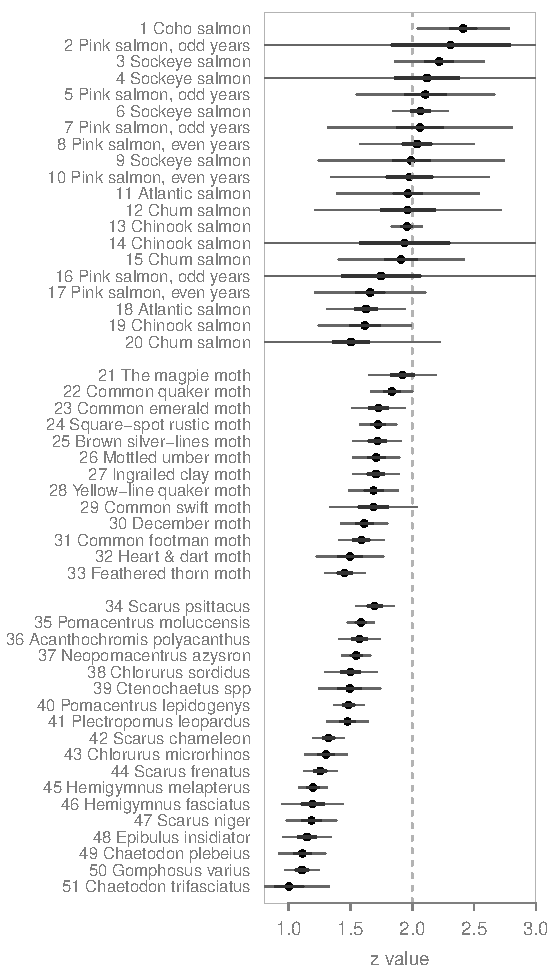
\includegraphics[height=6.6in]{prophets/Taylor_z_values.pdf}
  \caption[Taylor's power law z values across metapopulations.]{
    Taylor's power law z values across metapopulations. Points represent maximum
    likelihood estimates, thick line segments represent 50\% confidence
    intervals, and thin line segments represent 95\% confidence intervals. The
    vertical dashed line at z = 2 represents the value assumed by the average-CV
    PE method.
}
\label{fig:z-vals}
\end{figure}

\begin{figure}[htbp]
  \centering
  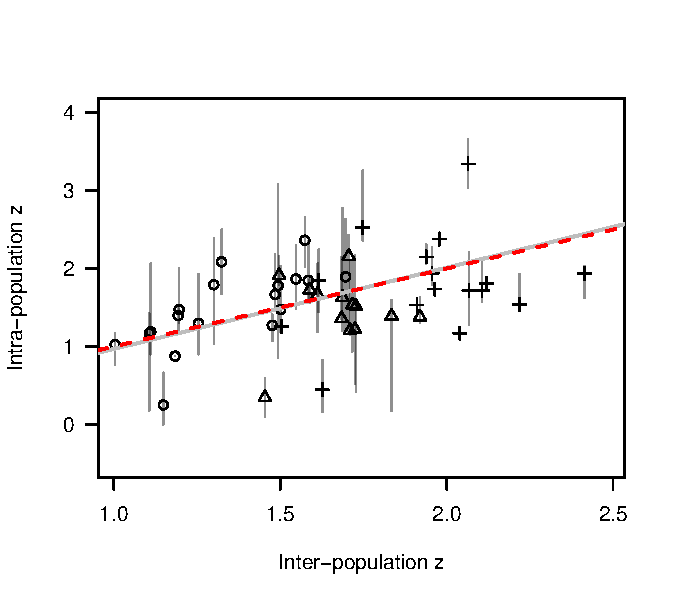
\includegraphics[width=4in]{prophets/inter-vs-intra-pop-z-seg-2-0-20121019.pdf}
  \caption[Intra- vs.\ inter-subpopulation mean-variance scaling relationship
    (Taylor's power law $z$-value).]{Intra- vs.\ inter-subpopulation mean-variance scaling relationship
    (Taylor's power law $z$-value).  Our estimation of the empirical
    mean-variance PE assumes that the inter-subpopulation $z$-value can
    approximate the intra-subpopulation $z$-value.  We use the
    inter-subpopulation $z$-value throughout our paper.  Here, we have also
    calculated the intra-subpopulation $z$-value for subpopulation time series
    in which the mean abundance in the 1\textsuperscript{st} or
    2\textsuperscript{nd} half of the time series is twice the magnitude of
    the other half.  Points represent median intra-subpopulation $z$-values
    within each metapopulation and vertical line segments represent
    1\textsuperscript{st} and 3\textsuperscript{rd} quartile values.  The
    dashed-red line represents a one-to-one relationship and the solid-grey
    line (under the one-to-one line) represents a linear regression of the
    median intra-subpopulation $z$-values with inter-subpopulation $z$-values.
    Symbols represent salmon (crosses), moths (triangles), and reef fishes
    (circles).}
  \label{fig:inter-vs-intra-z}
\end{figure}


\begin{figure}[htbp]
  \centering
  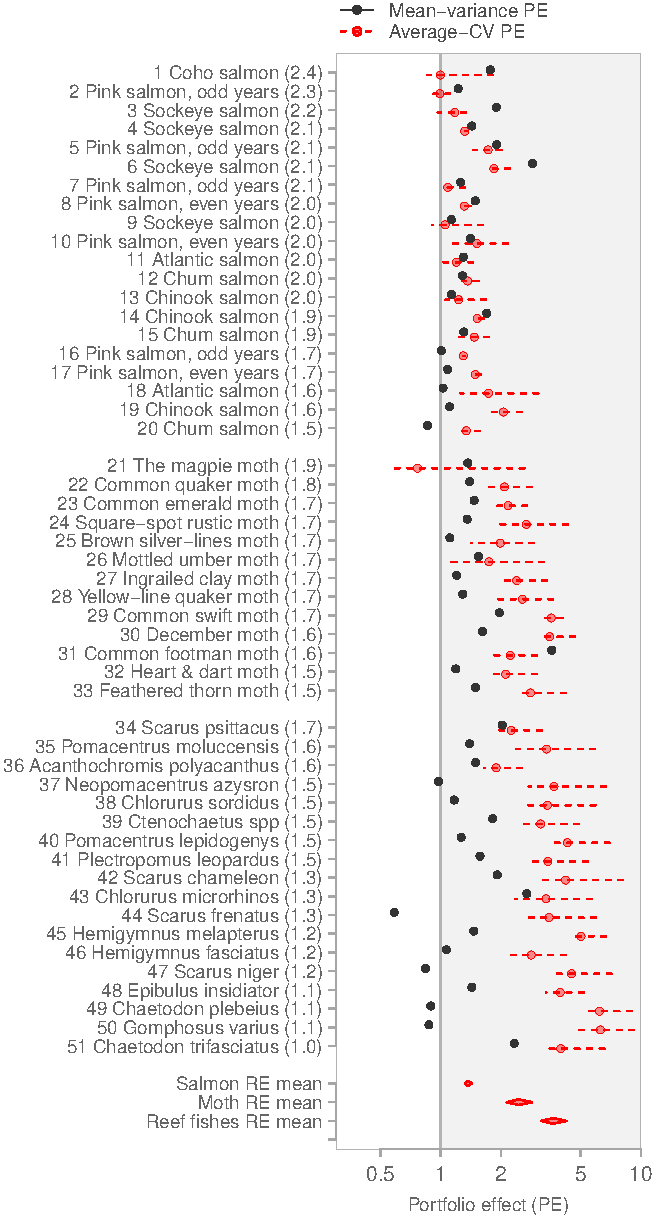
\includegraphics[height=6.8in]{prophets/PE_comparison_z_meta_taxa_quad_20121214.pdf}
  \caption[PEs with the mean-variance PEs estimated from a quadratic model.]{
    PEs with the \textbf{mean-variance PEs estimated from a quadratic model}.
    See Figure~\ref{fig:meta} for details.
}
\label{fig:meta-quad}
\end{figure}

\begin{figure}[htbp]
  \centering
  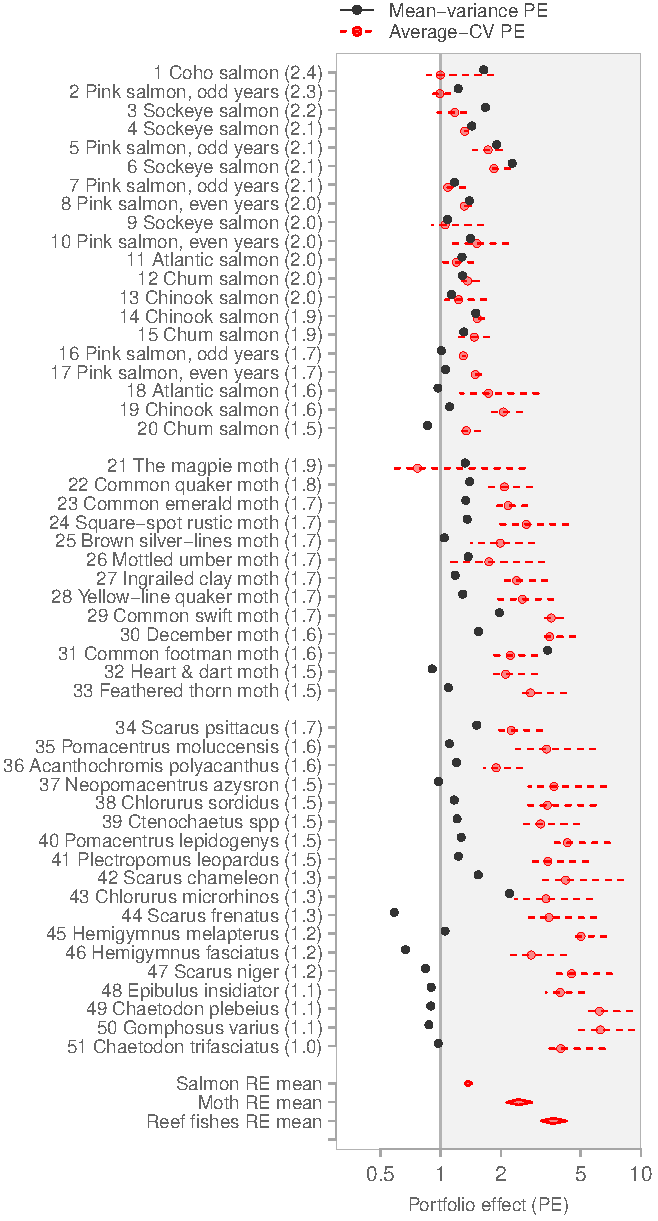
\includegraphics[height=6.8in]{prophets/PE_comparison_z_meta_taxa_lin_quad_avg_20121214.pdf}
  \caption[PEs with the mean-variance PEs estimated from a
      linear-quadratic averaged model.]{PEs with the \textbf{mean-variance PEs estimated from a
      linear-quadratic averaged model}. See Figure~\ref{fig:meta} for details.}
\label{fig:meta-lin-quad-avg}
\end{figure}

\begin{figure}[htbp]
  \centering
  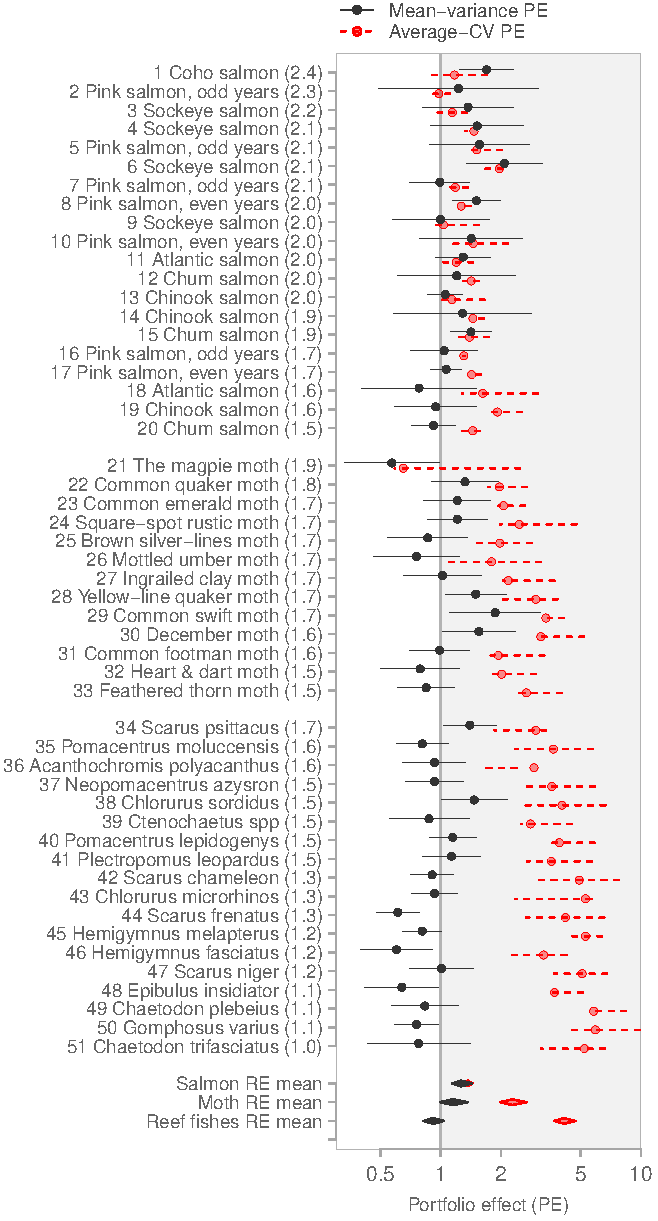
\includegraphics[height=6.8in]{prophets/PE_comparison_z_meta_detrend_taxa_20121214.pdf}
  \caption[PEs from linear detrended time series.]{PEs from \textbf{linear detrended} time series. See
    Figure~\ref{fig:meta} for details.
}
\label{fig:meta-detrend}
\end{figure}

\begin{figure}[htbp]
  \centering
  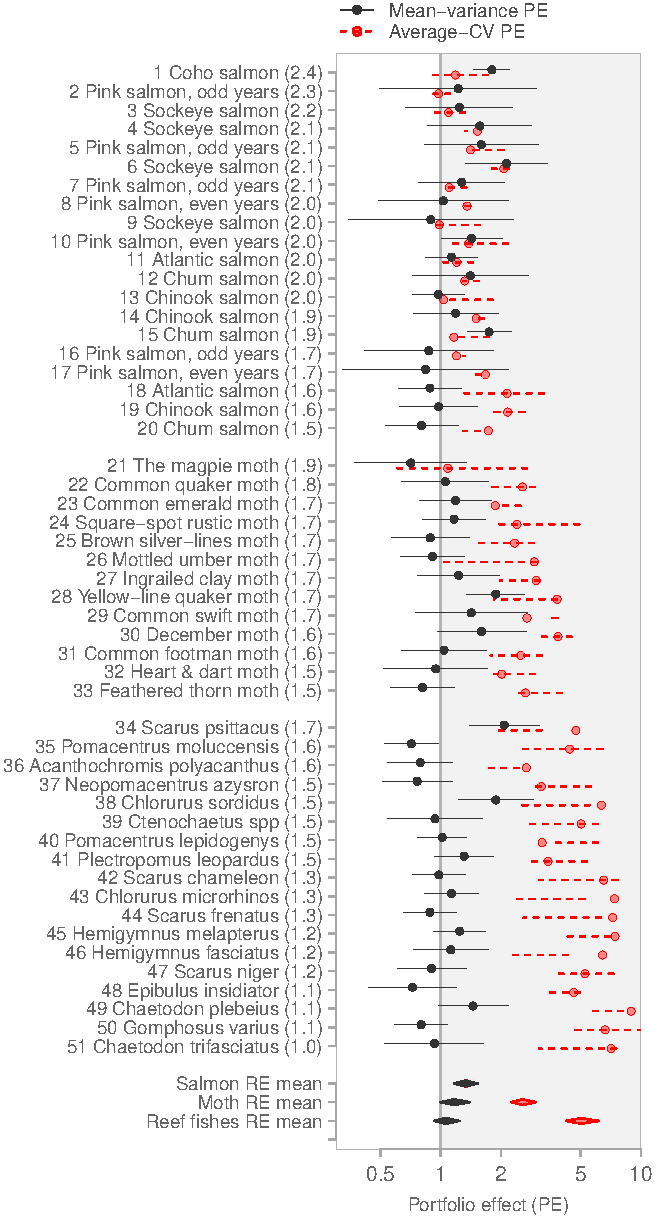
\includegraphics[height=6.8in]{prophets/PE_comparison_z_meta_loess_detrend_taxa_20121214.pdf}
  \caption[PEs from loess detrended time series]{PEs from \textbf{loess detrended} time series. See
    Figure~\ref{fig:meta} for details.
}
\label{fig:meta-detrend-loess}
\end{figure}
\clearpage

\begin{figure}[htbp]
  \centering
  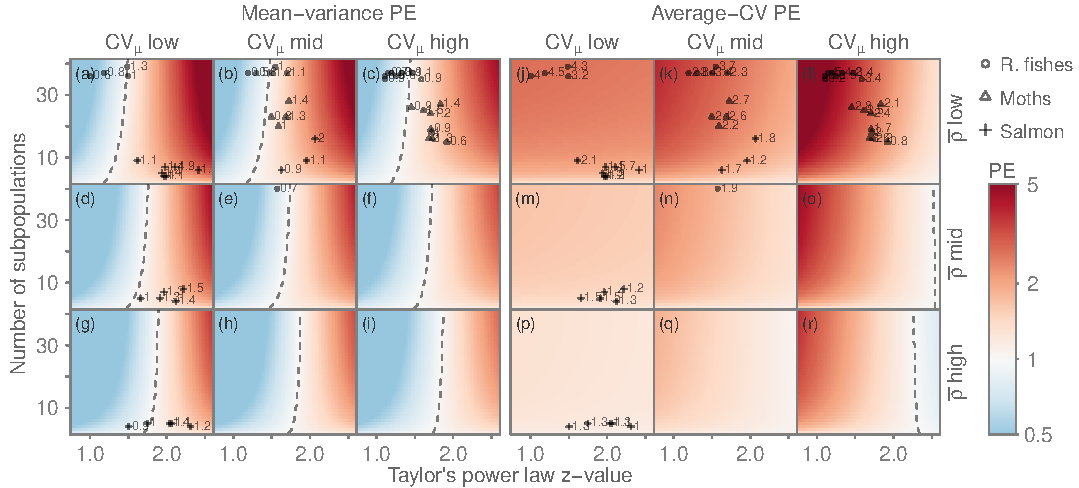
\includegraphics[width=\textwidth]{prophets/PE-parameter-space-labels-20120614.pdf}
  \caption[Empirical ecological PEs overlaid in theoretical PE
    parameter space.]{Empirical ecological PEs (points) overlaid in theoretical PE
    parameter space (colour shading). \textbf{This is the same as
    Figure~\ref{fig:paramspace} except that here we indicate the empirical PE values
      beside the points}. The colour shading indicates the
    stabilizing-effect of the theoretical mean-variance PEs (a--i) and
    average-CV PEs (j--r): red indicates a stabilizing effect and blue indicates
    a destabilizing effect.
    The dashed lines indicate neutral PEs. Columns from left to right
    show systems with increasingly uneven subpopulation sizes,
    and rows from top to bottom show systems with increasingly strong mean
    correlation between subpopulation
}
\label{fig:paramspace-labels}
\end{figure}
\clearpage

\begin{figure}[htbp]
  \centering
  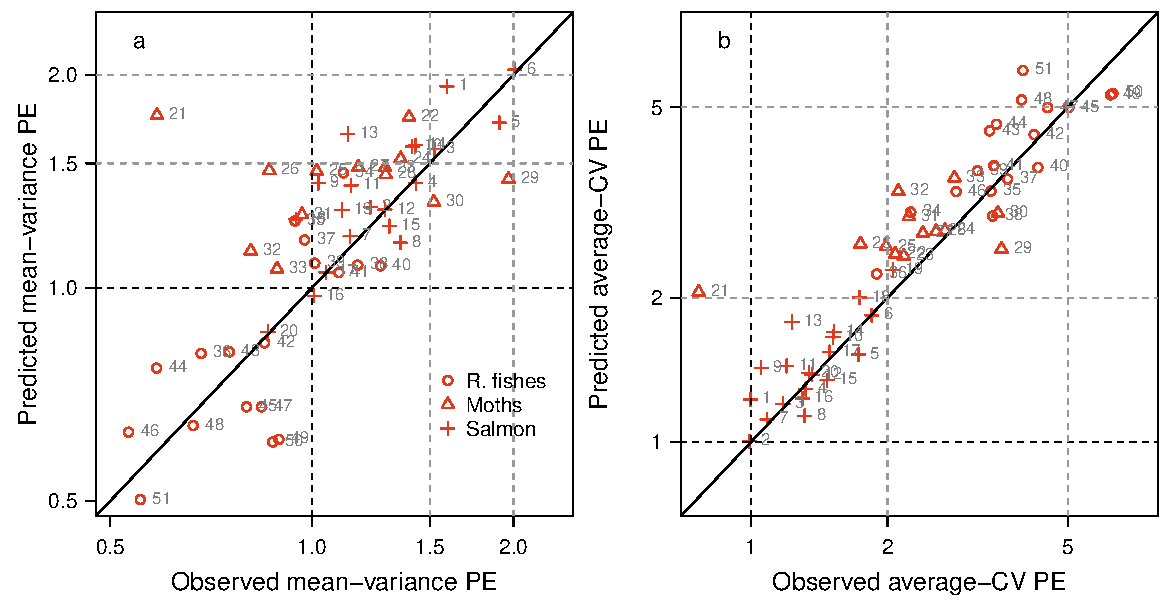
\includegraphics[width=\textwidth]{prophets/parameter-space-predicted-vs-observed-20120430.pdf}
  \caption[Predicted vs.\ observed mean-variance and average-CV
    PEs.]{ Predicted vs.\ observed mean-variance (\textbf{a}) and average-CV
    PEs (\textbf{b}).  Predicted PEs correspond to the colour underlying the
    metapopulations displayed in Figure~\ref{fig:paramspace}; observed PEs to
    the values calculated directly from the empirical data and shown in
    Figure~\ref{fig:meta}. The predicted PEs are approximate due to other
    statistical properties of the data beyond the four examined in
    Figure~\ref{fig:paramspace}, and due to grouping the $CV_{mu}$ and
    correlation values from the metapopulations to match the displayed
    theoretical values in the bins.  Numbers indicate the metapopulation IDs
    used throughout the paper (Table~\ref{tab:datasources}).  The solid sloped lines indicate
    one-to-one relationships.  Note that all axes have been log transformed
    and the two panels have separate axis limits.  }
  \label{fig:PE-predicted-observed}
\end{figure}

\begin{figure}[htbp]
  \centering
  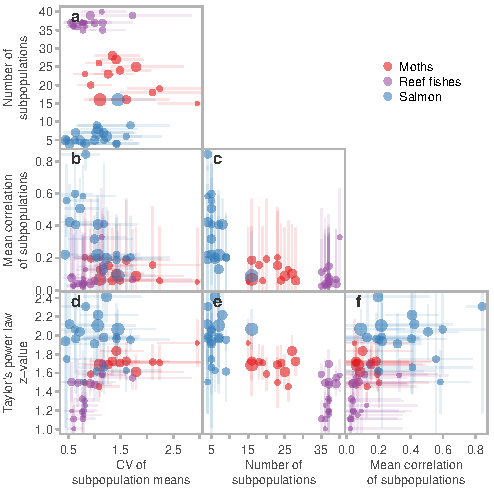
\includegraphics[height=4.6in]{prophets/bias_factors_cross_correlation.pdf}
  \caption[Relationship between the drivers of the PE in empirical systems for
    moths (red), reef fishes (purple), and salmon (blue).]{Relationship between the drivers of the PE in empirical systems for
    moths (red), reef fishes (purple), and salmon (blue).  The area of the
    filled circles corresponds to the strength of the \tilmanPE\ with larger
    circles corresponding to more stabilizing PEs.  Line segments indicate
    95\% confidence intervals.}
  \label{fig:factors-cor}
\end{figure}

\begin{figure}[htbp]
  \centering
  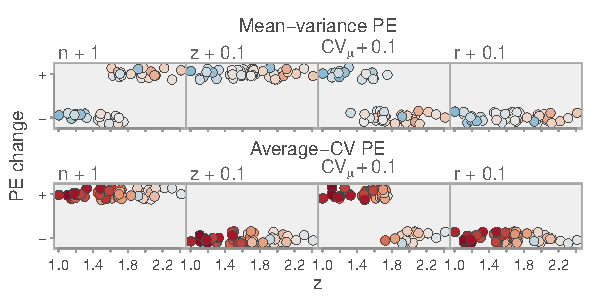
\includegraphics[width=5in]{prophets/PE-as-index.pdf}
  \caption[The PE used as an index of ecosystem change.]{ The PE used as an index of ecosystem change.  The upper panel
    shows the mean-variance PE and the lower panel the average-CV PE.  The
    horizontal axis shows Taylor's power law $z$-value.  The vertical axis
    shows the change in the PE (more stabilizing = $+$, less stabilizing =
    $-$).  The panels from left to right indicate an increase in the number of
    subpopulations ($n + 1$), Taylor's power law $z$-value ($z + 1$),
    subpopulation unevenness ($CV_{\mu} + 0.1$), or the correlation between
    subpopulations ($r + 0.1$). The quantities added are arbitrary and the
    results would look the same for any quantity added greater than zero.  Each
    dot represents an empirical metapopulation and the colour indicates the
    observed empirical PE using the same colour scale as Figs.~4~and~5. The dots
    are jittered vertically slightly for visual clarity.  }
  \label{fig:PE-as-an-index}
\end{figure}

%\end{spacing}

%\end{document}

\end{appendices}

\chapter[Metapopulation portfolio conservation]{Portfolio conservation of
  metapopulations under climate change\footnote{A version of this chapter
    appears as Anderson, S.C., J.W. Moore, M.M. McClure, N.K. Dulvy, A.B.
    Cooper. Portfolio conservation of metapopulations under climate change.
    Ecological Applications. In press.
    \url{http://doi.org/10.1890/14-0266.1}}}

\newcommand{\somR}{Appendix A}
\newcommand{\somparam}{Appendix B}
\newcommand{\somstray}{Appendix C}
\newcommand{\somsens}{Appendix D}
\newcommand{\somcor}{Appendix E}
\newcommand{\somts}{Appendix F}

\section{Abstract}\label{abstract}

Climate change will likely lead to increasing population variability and extinction risk. Theoretically, greater population diversity should buffer against rising climate variability, and this theory is often invoked as a reason for greater conservation. However, this has rarely been quantified. Here we show how a portfolio approach to managing population diversity can inform metapopulation conservation priorities in a changing world. We develop a salmon metapopulation model where productivity is driven by spatially-distributed thermal tolerance and patterns of short- and long-term climate change. We then implement spatial conservation scenarios that control population carrying capacities and evaluate the metapopulation portfolios as a financial manager might --- along axes of conservation risk and return. We show that preserving a diversity of thermal tolerances minimizes risk given environmental stochasticity and ensures persistence given long-term environmental change. When the thermal tolerances of populations are unknown, doubling the number of populations conserved may nearly halve metapopulation variability. However, this reduction in variability can come at the expense of long-term persistence if climate change increasingly restricts available habitat --- forcing ecological managers to balance society's desire for short-term stability and long-term viability. Our findings suggest the importance of conserving the processes that promote thermal-tolerance diversity, such as genetic diversity, habitat heterogeneity, and natural disturbance regimes, and demonstrate that diverse natural portfolios may be critical for metapopulation conservation in the face of increasing climate variability and change.

\noindent
%\textit{Keywords}: biocomplexity, ecosystem based management, Pacific salmon, portfolio effect, prioritization, range contraction, response diversity, risk assessment, stability-diversity, stochastic simulation

%\noindent
%\textit{Running head}: Metapopulation portfolio conservation

\section{Introduction}

Untangling the mechanisms that underpin the stability of ecological systems is a critical focus of ecology \citep[e.g.][]{ives2007, demazancourt2013}. Decades of research has focused on the role of species richness and functional diversity in driving stability; however, recent research has highlighted that the drivers of ecological stability are more complex and multidimensional than previously thought \citep[e.g.][]{balvanera2006, ives2007, demazancourt2013}. Two key drivers of population stability that have been comparatively understudied are response diversity \citep{winfree2009, mori2013} --- different responses to the environment by functionally similar species or populations \citep{elmqvist2003} --- and the role of metapopulations \citep{schtickzelle2007}. Here, we examine the role of response diversity conservation in stabilizing metapopulations given projected changes in climate. With unprecedented loss of biodiversity and levels of anthropogenic environmental change, it is more critical than ever to consider conservation approaches that maintain system stability in the face of environmental uncertainty \citep{lee2008, ando2012}.

Typically, conservation actions to maintain system stability and thereby reduce risk are driven by an \emph{ad hoc} combination of scientific information, political influences, and feasibility \citep{margules2000}; the management of financial portfolios provides another way of considering risk \citep[e.g.][]{figge2004, koellner2006, ando2012, haak2012}. Economists work to minimize risk and maximize returns by building a portfolio of individual investments (called assets) with different attributes. For example, different financial sectors can be expected to perform uniquely in some economic conditions; when one rises in value another may fall. Modern Portfolio Theory proposes that out of all possible portfolios, there is a small subset of portfolios that maximizes expected return for a level of risk or minimizes risk for a level of return (called the efficient frontier), and that only by considering risk and return in tandem can an investor achieve maximum benefit from a portfolio \citep{markowitz1952}.

Similarly, expected growth rate and variance of a metapopulation is a function of the variance, covariance, and size of the individual populations \citep{moore2010, carlson2011, anderson2013}. An ecological portfolio approach to managing risk for a metapopulation might therefore consider how conservation actions affect the weight of each population in a metapopulation portfolio. This investment weight could represent the conservation budget or the habitat conserved for each population. The population growth rate is then analogous to the financial rate of return and the variability of that growth rate a metric of risk. Environmental conditions could represent the financial market conditions. Given this interpretation, ecological managers could consider how various conservation strategies affect the expected risk and return of their ecological portfolio. These risk and return elements are central to ecological management and conservation --- management aims to ensure stability over environmental variability (risk), and increase population abundance (return). Different scenarios may suggest different desired trade-offs between the two. For example, a manager with a healthy population might prioritize short-term stability, while a manager with an endangered population might try to balance the two, or prioritize population growth initially.

Managing Pacific salmon under the uncertainty of climate change is an ideal scenario to consider through the lens of portfolio theory for four reasons. (1) The migration of Pacific salmon biomass profoundly influences aquatic and terrestrial coastal ecosystems throughout the North Pacific ocean from Korea to California \citep{quinn2005}. (2) Pacific salmon form metapopulations \citep[e.g.][]{policansky1998, cooper1999, schtickzelle2007} and we can consider, for example, the metapopulation in a river-catchment as a portfolio and the stream populations as assets \citep{schindler2010, moore2010, carlson2011, anderson2013, yeakel2014}. Fisheries often integrate across multiple populations, acting as investors in the salmon portfolio \citep{hilborn2003}. Fisheries managers and conservation agencies can act as portfolio managers by choosing which salmon habitat to prioritize for protection or restoration. (3) Many Pacific salmon metapopulations are highly threatened \citep[e.g.][]{gustafson2007} and will likely become more at risk as threats such as overfishing, damming, logging, and particularly changing climate, intensify \citep[e.g.][]{lackey2003}. Indeed, recovery goals for Pacific salmon are often set at the metapopulation level \citep{mcelhany2000}, and knowing what minimizes risk to the metapopulation can help choose efficient conservation actions \citep{policansky1998, mcelhany2000}. (4) Given the scale and variety of the threats facing salmon, some prioritization will be required to recover these highly-valued, even iconic species \citep{allendorf1997, ruckelshaus2002}.

Two key mechanisms can generate the asynchrony in metapopulation dynamics that is critical to a diversified portfolio. First, localized habitat features can filter larger-scale environments, generating unique conditions for populations \citep{schindler2008} (\emph{sensu} the Moran effect). Second, salmon populations may respond differently to environmental variability (i.e.~response diversity \citep{elmqvist2003} and biocomplexity \citep{hilborn2003}) arising from unique local adaptations and traits \citep{fraser2011, eliason2011, thorson2014}. In reality, these mechanisms can interact. For example, salmon response diversity in the marine environment can be driven by adaptation to localized freshwater environments \citep{johnson2013a}.

In addition to posing perhaps the greatest threat to global biodiversity in general \citep{thomas2004}, climate warming poses a particular threat to riverine species whose ranges are largely confined to existing habitat \citep{thomas2010}. Among these species, salmon are strongly affected by climate warming \citep[e.g.][]{patterson2007}. Warmer water can lead to massive mortality of salmon populations \citep[e.g.][]{patterson2007} and indirectly impact salmon productivity through alterations to snow-melt timing and extreme hydrological events \citep{crozier2008}. Due to these effects, adverse stream temperatures are already impeding recovery of some Pacific salmon populations \citep{mccullough1999} and are expected to make recovery targets more difficult to achieve \citep{battin2007}. However, despite the evidence that warming impacts salmon, salmon also show evidence of response diversity and local adaptation to temperature. For example, thermal tolerance of sockeye salmon in the Fraser River, British Columbia, Canada, varies within streams according to historical environmental conditions \citep{eliason2011}.

Here we ask how portfolio theory can inform spatial approaches to prioritizing metapopulation conservation in a changing world. To answer this, we develop a salmon metapopulation simulation in which spatially-distributed thermal tolerance and patterns of short- and long-term climatic change drive population-specific productivity. We then implement scenarios that prioritize alternative sets of populations and evaluate the salmon portfolios along risk-return axes, as a financial portfolio manager might. We show that conserving a diversity of thermal tolerances buffers metapopulation risk given short-term climate forcing and ensures metapopulation persistence given long-term climate warming. We then show that dividing conservation among more populations buffers risk regardless of thermal-tolerance diversity or climate trend, but possibly at the expense of long-term growth rate and persistence when available habitat declines over time. We conclude that considering metapopulations through portfolio theory provides a useful additional dimension through which we can evaluate conservation strategies.

\section{Methods}

We developed a 100-year salmon metapopulation simulation model that includes both population dynamics and harvesting along with process, observation, and implementation uncertainty (Fig.~\ref{f:flowchart}). We tested different conservation scenarios under two kinds of environmental regimes (short-term climate variability and long-term climate change) and in cases where habitat capacity remained constant or declined over time. We provide a package \texttt{metafolio} \citep{metafoliopkg} for the statistical software \textsf{R} \citep{r2013} as an appendix, to carry out the simulations and analyses described in this paper (\somR).

\subsection{Defining the ecological portfolio}\label{defining-the-ecological-portfolio}

In our ecological portfolios, we defined assets as stream-level populations and portfolios as salmon metapopulations. The specific configuration of our model refers to salmon that spend extended time rearing in freshwaters (e.g.~steelhead {[}\emph{Oncorhynchus mykiss}{]}, sockeye salmon {[}\emph{O. nerka}{]}, coho salmon {[}\emph{O. kisutch}{]}, and stream-type Chinook salmon {[}\emph{O. tshawytscha}{]}), which will likely be more impacted by changes to stream temperature and flow \citep{mantua2010}. We use the terms \emph{stream} and \emph{populations} interchangeably to represent the portfolio assets. We defined the portfolio investors as the stakeholders in the fishery and metapopulation performance. For example, the investors could be conservation agencies, First Nations groups, or civil society as a whole. The fisheries management agency then becomes the portfolio manager. We defined the asset value as the abundance of returning salmon in each stream and the value of the portfolio as the overall metapopulation abundance.

In this scenario, the equivalent to financial rate of return is the generation-to-generation metapopulation growth rate, calculated as the first difference of the log salmon returns. We defined the financial asset investment weights as the capacity of the stream populations --- specifically the unfished equilibrium stock size --- since maintaining or restoring habitat requires money, time, and resources and habitat size itself is a strong predictor of the occupancy of salmon \citep{isaak2007}. Investment in a population therefore represents investing in salmon habitat conservation or restoration and the risk and return from investment strategies become emergent properties of our metapopulation model.

\subsection{Salmon metapopulation dynamics}\label{salmon-metapopulation-dynamics}

The salmon metapopulation dynamics in our simulation were governed by a spawner-return relationship with demographic stochasticity and straying between populations. We defined the spawner-return relationship with a Ricker model,

\[R_{i(t+1)} = S_{i(t)}e^{a_{i(t)}(1-S_{i(t)}/b_i) + w_{i(t)}}\]

\noindent
where $i$ represents a population, $t$ a generation time, $R$ the number of returns, $S$ the number of spawners, $a$ the productivity parameter (which can vary with the environment), and $b$ the density-dependent term (which is used as the asset weights in the portfolios). The term $w_{i(t)}$ represents first-order autocorrelated error. Formally, $w_{i(t)} = w_{i(t-1)} \rho_w + r_{i(t)}$, where $r_{i(t)}$ represents independent and normally-distributed error with standard deviation of $\sigma_r$, mean of $-\sigma_r^2 / 2$ (bias corrected so the expected value after exponentiation is 1), and correlation between subsequent generation values of $\rho_w$. We set $\sigma_r = 0.7$ and $\rho_w = 0.4$ to match the mean values for salmonids in \citet{thorson2014a}.

We manipulated the capacity and productivity parameters $b_i$ and $a_{i(t)}$ as part of the portfolio simulation. The capacity parameters $b_i$ were controlled by the investment weights in the populations. For example, a large investment in a stream was represented by a larger unfished equilibrium stock size $b$ for stream $i$. The productivity parameters $a_{i(t)}$ were controlled by the interaction between a temperature time series and the population thermal-tolerance performance curves. In a different context, investment could represent improving the productivity ($a_i$) parameters, say through culling, to offset mortality increases due to changing temperatures. However, such a scenario is unlikely in the case of an endangered species where population levels are often well below levels where culling would increase productivity.

We generated the thermal-tolerance curves according to

\[a_{i(t)} = \begin{cases} a_i^{\mathrm{max}} -
W_i (e_t - e_i^{\mathrm{opt}})^2,
& \text{if } a_{i(t)} > 0\\ 0, & \text{if } a_{i(t)} \leq
0 \end{cases}\]

\noindent
where $W_i$ controls the width of the curve for population $i$, $e_t$ represents the environmental value at generation $t$, $e_i^{\mathrm{opt}}$ represents the optimal temperature for population $i$, and $a_i^{\mathrm{max}}$ represents the maximum possible $a$ value for population $i$. We set the $W_i$ parameters (evenly spaced values increasing and decreasing between 0.08 and 0.04) to generate widths approximately as shown in \citet{eliason2011}. We set the area under each curve to 30 units to create $a_i^{\mathrm{max}}$ values ranging roughly between 2.2 and 2.9 as in \citet{dorner2008}. These parameter values created some warm-tolerant populations, some cold-tolerant populations, and some populations with a wider range of thermal-tolerance but a lower maximum productivity (Fig.~\ref{f:curves}a). Although we refer to a thermal-tolerance curve because temperature is a dominant driver of salmon productivity \citep[e.g.][]{mccullough1999, patterson2007, eliason2011}, our model could apply to any environmental tolerance (e.g.~tolerance to stream flow volume or changes in snow melt timing; \citeauthor{crozier2008} \citeyear{crozier2008}).

We implemented straying as in \citet{cooper1999}. We arranged the populations in a line and salmon were more likely to stray to streams near their natal stream (\somstray). Two parameters controlled the straying: the fraction of fish $f_{\mathrm{stray}}$ (0.02) that stray from their natal stream in any generation and the rate $m$ (0.1) at which this straying between streams decays with distance

\[\mathrm{strays}_{ij(t)} = f_{\mathrm{stray}} R_{j(t)} \frac{e^{-m \lvert i-j
\rvert }} {\displaystyle\sum\limits_{ \substack{k = 1 \\ k \neq j}}^{n} e^{-m
\lvert k-j \rvert }}\]

\noindent
where $R_{j(t)}$ is the number of returning salmon at generation $t$ whose natal stream was stream $j$. The subscript $k$ represents a stream ID and $n$ the number of populations. The denominator is a normalizing constant to ensure the desired fraction of fish stray. Our simulation did not account for the homogenization of diversity due to straying. For example, all salmon in one population maintained the same thermal-tolerance curve regardless of how many salmon it received from another stream.

\subsection{Fishing}\label{fishing}

Our simulation used a simple set of rules to establish the exploitation rate of fisheries and the remainder left to spawn (escapement target). First, to establish a range of spawner-return values and to mimic the start of an open-access fishery, for the first 30 years we drew the fraction of fish harvested randomly from a uniform distribution between 0.1 and 0.9. We discarded these initial 30 years as a burn-in period. Then, every five years for the remaining 100 years of our simulation, we fitted a spawner-return function to the cumulative data for individual populations. The target escapement rate $E_{\mathrm{tar}}$ (a proportion per year) was set based on \citet{hilborn1992} as

\[E_{\mathrm{tar}} = \frac{R}{b (0.5 - 0.07a)} \label{eq:esc}\]

\noindent
where $R$ represents the return abundance and $a$ and $b$ represent the Ricker model parameters. The target harvest rate is then a function of returns and the escapement target ($H_{\mathrm{tar}} = R - E_{\mathrm{tar}}$). We included implementation uncertainty in the actual harvest rate $H_{\mathrm{act}}$ as a function of the target harvest rate and a beta distribution with location parameter $\alpha_h$, shape parameter $\beta_h$, and standard deviation of $\sigma_h$ (set to 0.1 as observed for similar data in \citet{pestes2008}).

\[\begin{aligned}
\alpha_h &= H_{\mathrm{tar}}^2 \left( \frac{1 -
H_{\mathrm{tar}}}{\sigma_h^2} - \frac{1}{H_{\mathrm{tar}}} \right)\\ \beta_h
&= \alpha_h \left({\frac{1}{H_{\mathrm{tar}}} - 1}\right)\\
H_{\mathrm{act}} &= \mathrm{beta}(\alpha_h, \beta_h).
\end{aligned}\]

\subsection{Environmental dynamics}\label{environmental-dynamics}

Environmental dynamics typically have both short- and long-term fluctuations, such as annual variability and directional climatic warming. We evaluated portfolio performance under these two components separately in our initial scenarios and combined in our final scenario. We did not explicitly model a cyclical climate trend, such as the Pacific Decadal Oscillation, but the effect of such a trend would largely be a product of the short-term variability and long-term trend. We represented short-term dynamics $e_{\mathrm{short}(t)}$ as a stationary first-order autoregressive process, AR(1), with correlation $\rho_e$ (0.1)

\[e_{\mathrm{short}(t)} = e_{t-1} \rho_e + d_t, d_t \sim \mathrm{N}(\mu_d, \sigma_d^2)\]

\noindent
where $d_t$ represents normally distributed deviations of some mean $\mu_d$ and standard deviation $\sigma_d$. We set $\mu_d$ to $16\,^{\circ}\mathrm{C}$ and $\sigma_d$ to $2\,^{\circ}\mathrm{C}$, to approximately match the stream temperature variation in \citet{eliason2011}. We represented long-term environmental dynamics $e_{\mathrm{long}(t)}$ as a linear shift in the temperature through time

\[e_{\mathrm{long}(t)} = e_0 + \beta_e t\]

\noindent
where $e_0$ represents the starting temperature up until the burn-in period ends and $\beta_e$ represents the annual increase in temperature. We set $e_0 = 15\,^{\circ}\mathrm{C}$ and $\beta_e = 0.04\,^{\circ}\mathrm{C} / \mathrm{generation}$ to obtain an increase in stream temperature of $4\,^{\circ}\mathrm{C}$ over the next century (assuming one generation equals one year) ending at or above the optimum thermal optimum of all populations. This increase approximately matches predicted increases in stream temperature --- relative to the 1980s, stream temperatures in the Pacific Northwest have already increased by approximately $0.2\,^{\circ}\mathrm{C}$/decade \citep{isaak2012}, and are predicted to increase $2$ to $5\,^{\circ}\mathrm{C}$ by 2080 \citep{mantua2010}.

We summarize the chosen parameter values in \somparam. Combining salmon population dynamics, fishing, and environmental dynamics, we illustrate the components of an example simulation in Fig.~\ref{f:ts} and the effect of varying population, fishing, and environmental parameters from their base values on metapopulation abundance in \somsens.

\subsection{Conservation scenarios}\label{conservation-scenarios}

\emph{Spatial conservation scenarios}: We evaluated four spatial conservation scenarios (Fig.~\ref{f:curves}b--e). We conserved four populations ($b_i = 1000$) and set the unfished equilibrium abundance of the six remaining populations to near elimination ($b_i = 5$) at the start of the simulation. These reduced populations could still receive straying salmon but were unlikely to rebuild on their own to a substantial abundance. The four spatial scenarios we considered were:

\begin{enumerate}
\def\labelenumi{\arabic{enumi}.}
\item
  Conserve a full range of thermal tolerances (conserve some cool-, some intermediate-, and some warm-tolerant populations; Fig.~\ref{f:curves}b).
\item
  Conserve the middle section of the metapopulation (conserve the most thermal-tolerant populations with the widest response curves; Fig.~\ref{f:curves}c).
\item
  Conserve the lower half of the metapopulation (conserve cool-tolerant populations; Fig.~\ref{f:curves}d).
\item
  Conserve the upper half of the metapopulation (conserve warm-tolerant populations; Fig.~\ref{f:curves}e).
\end{enumerate}

\emph{Unknown thermal tolerances}: In reality we rarely know precise levels of thermal response diversity. We therefore also considered cases where conservation was randomly assigned with respect to thermal tolerance but where conservation effort ($\sum\limits_{i=1}^n b_i = 2000$) could be distributed across different numbers of streams. We considered conserving from two to 16 streams with thermal tolerance distributed along the same range as in the spatial scenarios. As in the spatial strategies, we reduced the capacity of the remaining streams to the nominal level of $b_i = 5$.

\emph{Declining habitat availability}: Habitat capacity in the Pacific Northwest is likely shrinking over time as salmon populations are squeezed between warming temperatures reducing habitat from below and declining stream flows reducing the habitat that remains from above. For example, temperature isotherms are shifting upstream at 1--10 km/decade in low gradient streams that Chinook use for spawning \citep{isaak2013}. At the same time, summer-fall stream flow volumes have been decreasing 10--30\% across the Pacific Northwest over the past 50 years \citep{luce2009} and are likely to continue declining \citep{luce2013}. We therefore considered a scenario where habitat capacity declined by a constant amount across all populations. We reduced the $b$ parameters by 0.85 units per generation so that some of the smaller populations would reach near extinction by the end of the simulation, as is likely for smaller isolated populations within this century \citep[e.g.][]{gustafson2007}. In this scenario, we considered cases where thermal tolerance was unknown but conservation effort could be distributed across between 16 and two streams. Climate followed a combination of the same long-term warming and short-term variability as before. For many Pacific salmon metapopulations, this scenario represents the most realistic scenario investigated.

\section{Results}

\subsection{Spatial conservation scenarios}\label{spatial-conservation-scenarios}

\emph{Given short-term environmental fluctuations} (strong interannual variation), conserving a wide range of thermal tolerances is the safest choice because it reduces overall risk to an ecological portfolio (Fig.~\ref{f:sp}a; \somts~Figs.~\ref{f:eg-sp-arma-full}, \ref{f:eg-sp-arma-half}). The average variance of metapopulation growth rate was 1.6 times lower given balanced thermal tolerance conservation (conserving a full range of thermal tolerances or the middle section vs.~the upper or lower half). Thermal tolerance diversity also led to more consistent stability --- there was less spread in variance across simulated metapopulations (width of quantiles from left to right in Fig.~\ref{f:sp}a). These increases in stability occurred despite the portfolios being comprised of warm- and cool-thriving populations that individually showed greater variation in response to environmental variability than populations with wide thermal tolerance curves. We can see the mechanism behind these portfolio properties by inspecting example population time series (Fig.~\ref{f:sp}c, d). If only the upper or lower half of thermal tolerances is conserved, the portfolio tends to alternate between performing well and poorly, depending on the environmental conditions, resulting in a riskier portfolio (Fig.~\ref{f:sp}e). This risk is buffered when a diversity of thermal tolerances is conserved (Fig.~\ref{f:sp}c) and the resulting asynchrony in population abundance (\somcor).

\emph{Given long-term environmental change}, such as climate warming, an ecological manager is hedging his or her bets on the environmental trend and how the populations will respond by conserving a range of thermal tolerances. The choice of which populations to conserve affects the ``rate of return'' (metapopulation growth rate) properties of an ecological portfolio (Fig.~\ref{f:sp}b; \somts~Figs.~\ref{f:eg-sp-linear-full}, \ref{f:eg-sp-linear-half}). The typical metapopulation growth rate when thermal tolerances were balanced was near zero --- the metapopulation neither increased nor decreased in abundance in the long run. The example metapopulation abundance time series (Fig.~\ref{f:sp}d, f) illustrate the mechanism: by conserving a range of thermal tolerances, when one population is doing poorly, another is doing well and the metapopulation abundance remains stationary through time. If a manager had invested only in the populations that were doing well at the beginning they would have had the lowest metapopulation growth rate at the end (purple portfolios in Fig.~\ref{f:sp}f).

\subsection{Unknown thermal tolerances}\label{unknown-thermal-tolerances}

In a scenario where the distribution of population-level thermal tolerances are unknown, portfolio optimization informs us that investing in more populations buffers portfolio risk regardless of environmental trend (Fig.~\ref{f:n}). \emph{Given short-term environmental fluctuations}, conserving more populations buffers portfolio risk (Fig.~\ref{f:n}a, c, d; \somts~Figs.~\ref{f:eg-n-arma-two}, \ref{f:eg-n-arma-sixteen}). For example, a metapopulation with 16 conserved populations is on average 1.7 times less variable than a metapopulation with only eight. At the same time, the random conservation of thermal tolerances creates an increased spread of possible metapopulation risk given fewer populations conserved (increasing quantile width from left to right in Fig.~\ref{f:n}a).

\emph{Given long-term environmental change}, conserving more populations also buffers portfolio risk (Fig.~\ref{f:n}b; \somts~Figs.~\ref{f:eg-n-linear-two}, \ref{f:eg-n-linear-sixteen}). Furthermore, in comparison to the short-term environmental noise scenario, the long-term environmental change creates a greater spread of possible metapopulation growth rates. For example, the height of the 75\% quantile of the mean metapopulation growth rate for the two-population systems (light grey polygons) is larger given long-term change than short-term change.

\subsection{Declining habitat availability}\label{declining-habitat-availability}

Given a reduction in stream flow over time along with climate change and climate variability, a manager encounters a risk-return trade-off when deciding how many populations to distribute conservation efforts across (Fig.~\ref{f:squeeze}; \somts~Figs.~\ref{f:eg-n-squeeze-two}, \ref{f:eg-n-squeeze-twelve}). Conserving more populations buffers portfolio risk, but at the expense of expected metapopulation growth rate. For example, the mean metapopulation variance was 2.7 times lower when 12 populations were conserved instead of four, but the expected metapopulation growth rate was 2.0 times lower when 16 populations were conserved instead of eight. The conservation scenarios represent an efficient frontier where a manager must choose whether to hedge his or her bets on a smaller number of populations and take on greater expected variability or conserve more populations and accept a lower expected metapopulation growth rate.

\section{Discussion}

The importance of conserving populations with a diversity of responses to the environment is a key assumption of conservation ecology, but has rarely been tested quantitatively \citep{mori2013}. We show how maintaining populations with a variety of thermal tolerances reduces risk caused by short-term environmental stochasticity and optimizes chances for long-term persistence given climate change. Further, conserving more populations reduces metapopulation variability but possibly at the expense of long-term metapopulation growth rate if available habitat is squeezed by climate change. In this discussion, we begin by linking our model with real-world conservation issues for Pacific Northwest salmon. We then consider broader implications for metapopulation conservation of any species and ecological stability in general.

\subsection{Implications for salmon conservation}

Our results emphasize the importance of promoting ecological conditions that promote diversity of environmental response to the environment if stability is to be maintained in the face of environmental uncertainty. This suggests three clear conservation actions. First, since habitat heterogeneity can lead to local adaptation \citep[e.g.][]{fraser2011}, our results emphasize the need to maintain a diversity of salmon habitat \citep{rogers2008}. Second, if conservation actions must be prioritized, then our model suggests we should focus on populations that aren't spatially contiguous to maximize diversity of response to the environment. Third, our results demonstrate the advantages of avoiding structures that artificially remove diversity of environmental response. For salmon, dams are a prominent example \citep{mcclure2008a}. Dams can have a double impact whereby their introduction selectively eliminates a large swath of contiguous habitat, perhaps analogous to our upper- or lower-half scenarios in Fig.~\ref{f:sp}, and then mitigation approaches such as hatcheries can further reduce response diversity if not carefully managed \citep{mcclure2008b}. In fact, salmon habitat lost to dams in the western U.S. has been biased towards warmer, drier, higher habitats \citep{mcclure2008a} and our findings suggest the resulting loss of warm-tolerant species may compound the risk to current metapopulations in the face of global warming.

The goals of existing salmon management structures in the western US and Canada support a portfolio conservation perspective. In the US, salmon populations are divided into Evolutionarily Significant Units (ESUs), groups of populations that are reproductively isolated and share a common evolutionary heritage, and finer-scale Viable Salmonid Populations (VSPs), populations that are demographically independent of other populations over a 100-year time frame \citep{mcelhany2000}. In Canada, the rough equivalent to the ESU is a Conservation Unit (CU), which consists of a group of salmon that are reproductively isolated and that if lost would be unlikely to recolonize in a reasonable time frame \citep{dfo2005wsp}. A salmon portfolio in our model could represent an ESU or CU and the lessons learned from our models are thus directly applicable to management guidelines in the Pacific Northwest. In fact, a number of VSP guidelines agree with our findings. For example, VSP guidelines suggest maintaining diversity in a variety of forms, focusing conservation efforts not just where salmon are currently abundant, and maintaining metapopulations with some populations near each other and others further apart \citep{mcelhany2000}.

However, salmon populations in the Pacific Northwest are already heavily impacted \citep[e.g.][]{gustafson2007} and VSP and CU recovery goals have not yet been achieved for most populations. Since European-Americans arrived, 29\% of 1400 historical salmon populations in the Pacific Northwest and California have been lost \citep{gustafson2007}. Furthermore, 44\% of salmon habitat in the western US (in the lower 48 states) has been lost to dams and other freshwater blockages \citep{mcclure2008a}. Changes to habitat, combined with increasing climate variability, has led to disturbance regimes that differ substantially in the frequency, magnitude, and duration from historical patterns, and threaten the resilience of salmon populations \citep{waples2009}. Many remaining populations rely on hatcheries for long-term population viability --- creating substantial evolutionary risks such as outbreeding depression, genetic homogenization, reduced effective population size, and domestication of fish (adaption to artificial environments and reduced fitness in wild environments) \citep{mcclure2008b}. Reduction of long-term reliance on hatcheries, accompanied by habitat restoration through, for example, restoring connectivity of floodplains and stream flow regimes, remains a critical component of long-term salmon sustainability in the Pacific Northwest --- particularly given predicted patterns of climate change \citep{beechie2013}.

Our model complements other simulation-based salmon-habitat prioritization models. While these other models tend to focus on detailed assessment of individual fish stocks, our model is the first to consider the role of response diversity in buffering risk for metapopulations as a whole. The Shiraz model is one complementary prioritization scheme \citep{scheuerell2006}. It focuses on detailed conditioning of the habitat-population-dynamics relationship at multiple life-history stages for a single salmon population. Whereas the Shiraz model can be applied to an entire watershed, it combines the populations together as a single unit thereby ignoring the role of population-level environmental response diversity. A second salmon prioritization model proposes combining population viability measures with an assessment of the genetic consequences of losing particular populations \citep{allendorf1997}. This model, however, also focuses on the assessment of individual stocks without considering their covariance and therefore the performance of the salmon portfolio as a whole. Our model does not replace these prioritization schemes. Rather, it proposes an additional focus on prioritization that optimizes metapopulation growth \emph{and} risk and that considers diversity of tolerance to environmental conditions.

While our model captures many relevant aspects of salmon life history and environmental dynamics, it ignores others that could be investigated in future analyses and might improve our understanding of salmon portfolio conservation. First, some salmon populations, such as ocean-type Chinook, tend to spawn further downstream than stream-type salmon. Ocean-type Chinook may therefore be less affected by declining stream flow and be able to shift upstream to avoid shifting isotherms \citep{mantua2010}. A model could consider evolutionary adaptation by having populations adopt more ocean-type-like characteristics. Second, our model ignores lost thermal-tolerance diversity from populations that reach low population sizes and are reestablished by straying from nearby streams. An individual-based model might more accurately penalize for this lost diversity and emphasize the need to define lower limits on the investment weights in a salmon conservation portfolio. Third, our model ignores fine-scale within-stream spatial and temporal environmental fluctuations. Fine-scale extremes in temperature and stream flow may be particularly important to population dynamics \citep{mantua2010} and could be incorporated into a future analysis. Such a model might show an increased benefit of portfolio optimization if the impact of increased magnitude and frequency of local climate extremes is important in addition to the mean trend \citep{jentsch2007}.

\subsection{Broad ecological implications and conservation priorities}\label{broad-ecological-implications-and-conservation-priorities}

To promote the stabilizing effect of a diversified ecological portfolio, there are two key components to identify: (1) the environmental drivers to which a varied response might occur, and (2) the conservation actions that can increase or decrease the diversity of response. A third component, identifying the traits and behaviours that mediate population responses to the environment may provide further insight into the mechanisms. Environmental drivers of response can include, for example, changes to temperature, habitat availability, air quality, water chemistry, or extreme weather \citep{elmqvist2003}. Identifying conservation actions that promote environmental response diversity is critical to developing stable ecological systems \citep{mori2013}. However, merely measuring environmental response diversity in real ecological systems is challenging \citep[albeit possible;][]{thibaut2012}. Therefore, one realistic solution may be to create general guidelines from a small number of intensively-monitored systems in which we can associate changes in synchrony of populations with changes in conservation regimes \citep[e.g.][]{moore2010, carlson2011}. Another solution may be to monitor the diversity of environmental conditions themselves (e.g.~temperature, stream flow, and gravel size in the case of salmon) since we know that traits affecting response to environmental conditions are heritable and are likely to adapt to local conditions \citep{carlson2011} possibly producing diversity of response to subsequent disturbances.

We suggest a number of specific extensions to our simulation model. First, the environment-thermal-tolerance mechanism could be expanded --- the distribution of environmental tolerance across a metapopulation does not necessarily follow a linear gradient, different forms of environmental tolerance could interact, and environmental conditions could affect populations through mechanisms other than productivity. Second, in addition to other taxa, our model could be extended to ecological communities or meta-communities after accounting for species interactions. Third, without any modifications, our model could consider the Moran or environmental-filter concept whereby populations experience increasingly different environmental forces at further distances \citep{schindler2008, rogers2008}. Fourth, a model could consider the contribution of contemporary evolution \citep{stockwell2003}. These rapid adaptations to changes in the environment could strongly influence portfolio performance and emphasize the importance of maintaining genetic diversity and a variety of local habitat. Finally, our model could be conditioned on a system of interest --- say a particular river basin in our example --- and the metapopulation portfolio could be optimized across conservation and restoration options as part of a formal decision analysis.

Management decisions for exploited species often come with a trade-off between conservation and revenue generation. Our findings when habitat capacity declined over time illustrate another kind of trade-off more similar to the trade-off described by \citet{markowitz1952} in his seminal financial portfolio work. In this case, managers must navigate a trade-off between expected risk and return of the metapopulation/portfolio growth rate itself. No position along this trade-off is inherently better than another unless considered in the context of societal values. Does society value short-term stability or a greater assurance of long-term persistence? The optimal choice likely lies somewhere in the middle and parameterizing our model to a specific metapopulation could illustrate the nature of the trade-off and aid conservation decision making. However, if environmental tolerance could be targeted for conservation as in Fig.~\ref{f:sp}, a manager could likely achieve portfolios closer to the efficient frontier in Fig.~\ref{f:squeeze}. In other words, a manager could achieve a lower expected variance for the same expected growth rate or a higher expected growth rate for the same expected variance --- a better conservation outcome in either case.

Conservation planning is inherently a spatial activity \citep{pressey2007} and our results can inform how we approach spatial conservation planning. First, our results suggest focusing on conserving the processes and mechanisms underlying stability, not just biodiversity itself \citep{pressey2007, beechie2013}. In particular, our results suggest that response diversity should be a mainstream element of conservation, not just species and functional diversity \citep{mori2013}. Our analysis also illustrates how conserving a portfolio of populations, ideally selected for a wide range of environmental tolerance, can help integrate across environmental uncertainty when spatial planning \citep{ando2012}. This is particularly important given the uncertainty surrounding the future ecological responses to climate change \citep{walther2002}. Finally, the increasing rapidness and variability of environmental change necessitates a dynamic approach in which spatial planning is reevaluated at regular intervals \citep{hannah2002a} --- perhaps testing for changes in population and species asynchrony in addition to changes in local productivity and variability. Combined, our results detail a pathway through which population diversity in environmental tolerance can underpin the stability of ecological systems. This pathway highlights that diverse natural portfolios may be critical for the conservation of metapopulations in the face of increasing climate variability and change.

\section{Acknowledgements}

We thank T.A. Branch, J.D. Yeakel, S.M. O'Regan, S.A. Pardo, L.N.K. Davidson, and C.C. Phillis for helpful discussions and comments on earlier drafts. We thank D.J. Isaak, an anonymous reviewer, and O.P. Jensen for suggestions that greatly improved the manuscript. We are particularly grateful to D.J. Isaak for suggesting and carefully outlining the declining stream flow scenario. Funding was provided by Simon Fraser University, NSERC (ABC, NKD, SCA), the Canada Research Chairs Program (NKD), the Liber Ero Chair of Coastal Science and Management (JWM), Fulbright Canada (SCA), and a Garfield Weston Foundation/B.C. Packers Ltd. Graduate Fellowship in Marine Sciences (SCA).

\begin{figure}[htbp]
\centering
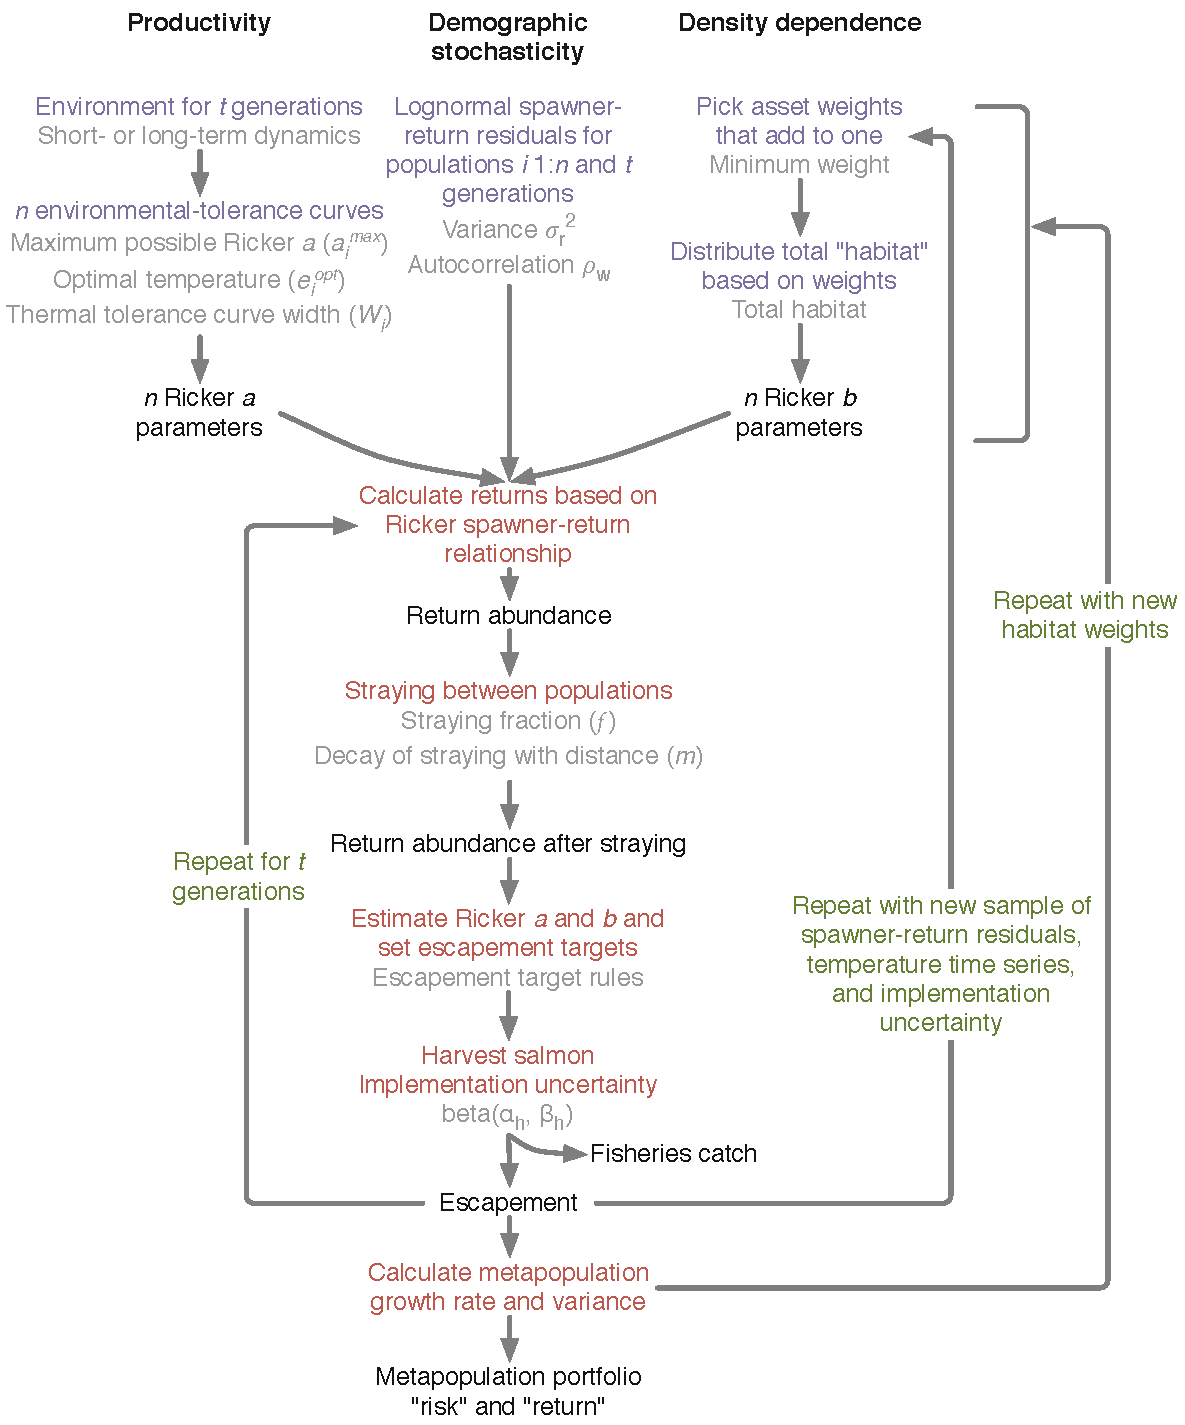
\includegraphics[width=5in]{metafolio/Fig1.pdf}
\caption{
Flow chart of the salmon-metapopulation simulation.
} \label{f:flowchart}
\end{figure}


\begin{figure}[htbp]
\centering
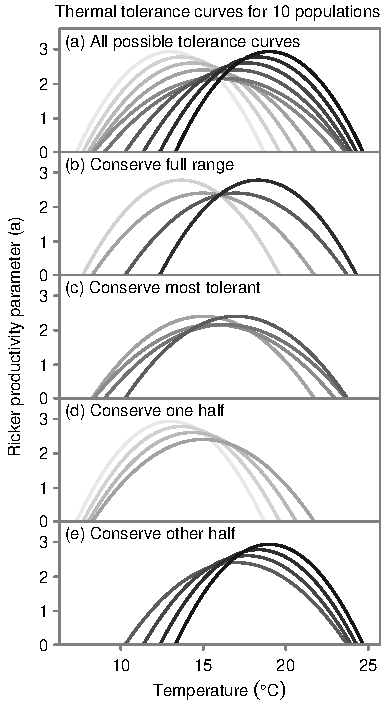
\includegraphics[width=2.9in]{metafolio/Fig2}
\caption{Different ways of prioritizing thermal-tolerance conservation. Panel a shows thermal-tolerance curves for ten possible populations and panels b--e show different ways of prioritizing four of those populations. The curves describe how productivity varies with temperature for a given population. Some populations thrive at low temperatures (light greys) and some at warm temperatures (dark greys). Some are tolerant to a wider range of environmental conditions (mid greys) but with a lower maximum productivity. The total possible productivity (the area under the curves) is the same for each population.} \label{f:curves}
\end{figure}


\clearpage

\begin{figure}[htbp]
\centering
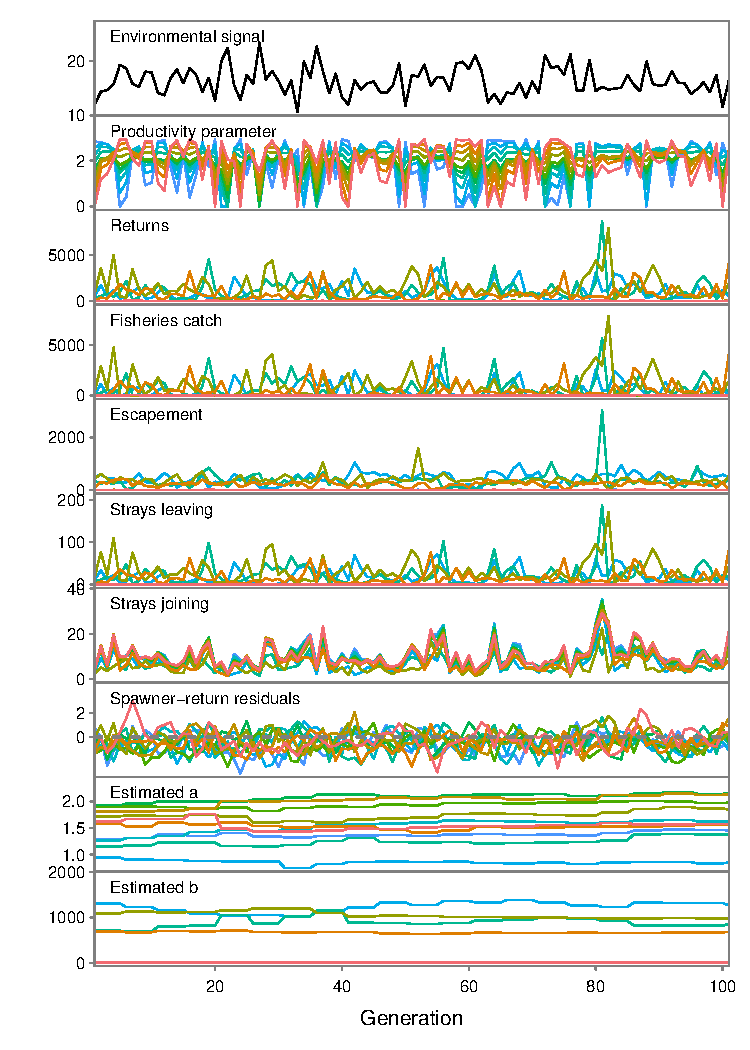
\includegraphics[width=4.0in]{metafolio/Fig3}
\caption{The components of an example metapopulation simulation. We show, from top to bottom, the temperature signal, the resulting productivity parameter (Ricker $a$), the salmon returns, fisheries catch, salmon escapement, salmon straying from their natal streams, salmon joining from other streams, spawner-return residuals on a log scale, and the estimated $a$ and $b$ parameters in the fitted Ricker curve. The shaded lines indicate populations that thrive at low (light grey) to high (dark grey) temperatures.} \label{f:ts}
\end{figure}

\clearpage

\begin{figure}[htbp]
\centering
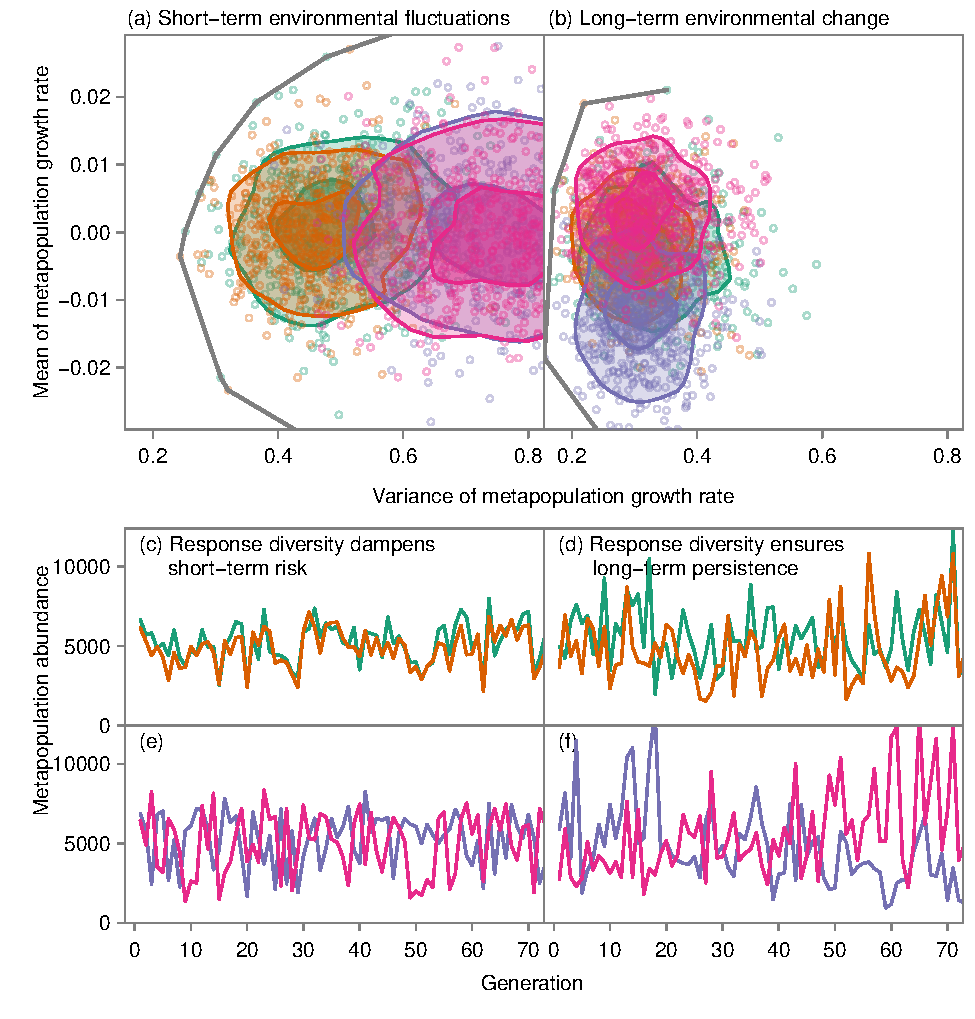
\includegraphics[width=4.5in]{metafolio/Fig4}
\caption{The importance of preserving thermal-tolerance diversity through spatial conservation strategies. The conservation strategies correspond to figure 2 and represent conserving a range of responses (green), the most stable populations only (orange), or one type of environmental response (purple and pink). In risk-return space we show environmental scenarios that are comprised primarily of (a) short-term and (b) long-term environmental fluctuations. The dots show simulated metapopulations and the contours show 25\% and 75\% quantiles across 500 simulations per strategy. We also show example metapopulation abundance time series for the (c, e) short-term and (d, f) long-term environmental-fluctuation scenarios. The thick grey line (a, b) indicates the efficient frontier across all simulated metapopulations --- metapopulations with the minimum variability for a given level of growth rate.} \label{f:sp}
\end{figure}

\clearpage

\begin{figure}[htbp]
\centering
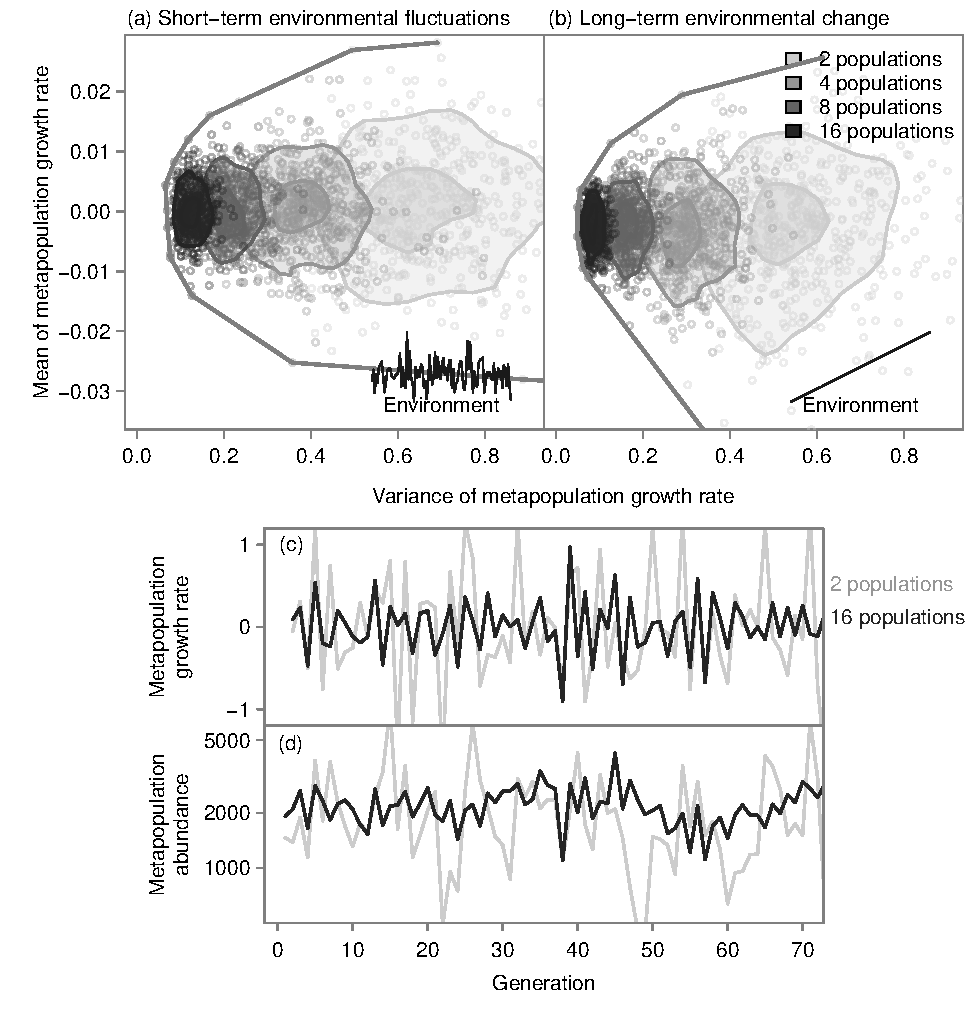
\includegraphics[width=4.5in]{metafolio/Fig5}
\caption{The importance of preserving as many populations as possible when we do not know how thermal-tolerance is distributed. In risk-return space we show environmental scenarios that are comprised primarily of (a) short-term and (b) long-term environmental fluctuations. We show metapopulations in which two through 16 populations are conserved. The dots show simulated metapopulations and the contours show 25\% and 75\% quantiles across 500 simulations per strategy. We also show example metapopulation (c) rate-of-change and (d) abundance time series for the short-term environmental-fluctuation scenario. The thick grey line (a, b) indicates the efficient frontier across all simulated metapopulations --- metapopulations with the minimum variability for a given level of growth rate.} \label{f:n}
\end{figure}

\clearpage

\begin{figure}[htbp]
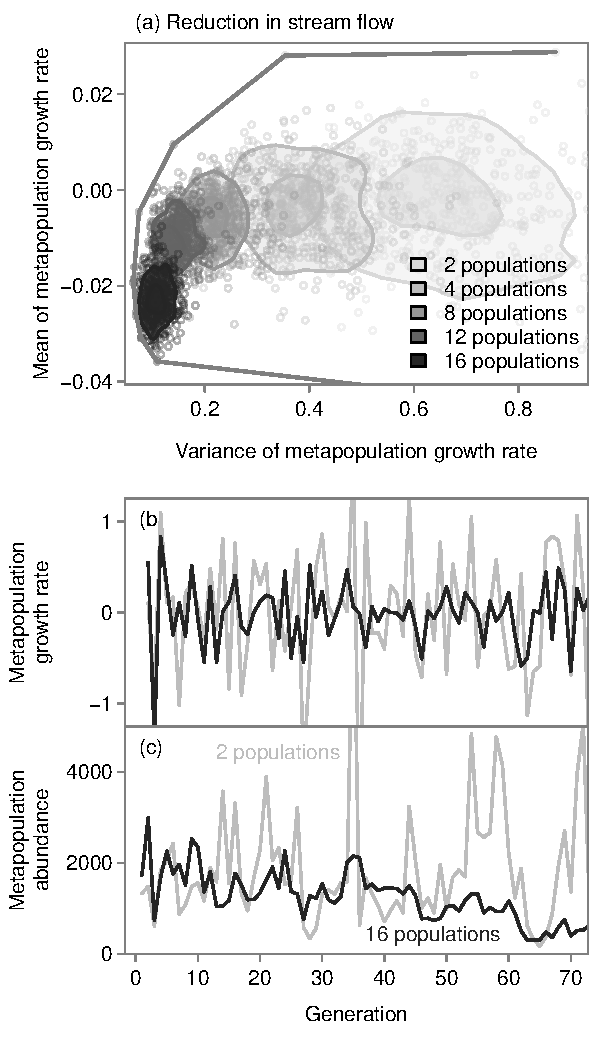
\includegraphics[width=3.0in]{metafolio/Fig6}
\centering
\caption{Risk-return trade-off in the case where habitat is lost over time through stream flow reduction. The temperature follows both short-term fluctuations and a long-term increase. Thermal tolerance is randomly conserved. Shading indicates conservation plans where two through 16 populations are conserved. (a) Conserving more populations decreases expected variance but also decreases expected growth rate. Dots show simulated metapopulations and contours show 25\% and 75\% quantiles across 500 simulations per strategy. The thick grey line indicates the efficient frontier across all simulated metapopulations --- metapopulations with the minimum variability for a given level of growth rate. Also shown are (b) example metapopulation growth rate and (c) abundance time series from the 2 and 16 population scenarios. Regression lines in (b) illustrate a decreasing growth rate through time.} \label{f:squeeze}
\end{figure}

\begin{appendices}
\chapter[Supporting materials]{Supporting materials for Portfolio conservation of metapopulations}

%\textsc{Appendix A.} The \texttt{metafolio} \textsf{R} package.

\noindent
The \texttt{metafolio} \textsf{R} package contains the functions and
code to carry out the analyses in our paper. \texttt{metafolio}. The
package can be installed from CRAN with:

\begin{verbatim}
install.packages("metafolio")
\end{verbatim}

\noindent
Alternatively, you can view the code and install the package from\\
\texttt{http://github.com/seananderson/metafolio}.

\noindent
The included vignette describes the package and illustrates some example
simulations. You can view the vignette with:

\begin{verbatim}
vignette("metafolio")
\end{verbatim}

\noindent
You can view the help for the package with:

\begin{verbatim}
?metafolio
help(package = "metafolio")
\end{verbatim}

\noindent
The figures from this paper can be re-created by downloading the code
from GitHub and sourcing the file \texttt{README.R} in the
\texttt{inst/examples} folder:

\begin{verbatim}
setwd("metafolio/inst/examples")
source("README.R")
\end{verbatim}

\clearpage

%\textsc{Appendix B.} Simulation input parameters and default values.

\bibliographystyle{apalike}
\bibliography{/Users/seananderson/Dropbox/tex/jshort,/Users/seananderson/Dropbox/tex/ref3}
\clearpage

\section{Supporting Tables and Figures}
%\begin{table}[h!]
%\centering
%\small
%\caption{Components of salmon metapopulation portfolios KEEP THIS?}
%\begin{tabular}{p{3.6cm}p{7.5cm}}
%\toprule
%Component          & Definition for the salmon portfolio\\
%\midrule
%Assets             & Stream-level salmon populations; possibly a Viable Salmonid Population\\
%Portfolio          & The salmon metapopulation; possibly an Evolutionarily Significant Unit\\
%Portfolio managers & Salmon managers\\
%Investors          & Salmon managers, conservation agency, or salmon fishers\\
%Asset weights      & Carrying capacity (specifically the $b$ parameters in a Ricker model)\\
%Asset returns      & Rate of change of generation-to-generation salmon metapopulation abundance\\
%Asset risk         & Variance of generation-to-generation salmon metapopulation abundance\\
%\bottomrule
%\end{tabular}
%\label{t:port}
%\end{table}
%\clearpage

\begin{table}[h!]
\centering
\footnotesize
\caption{Input parameters to the salmon metapopulation simulation with default values.}
\smallskip
\begin{tabular}{>{\RaggedRight}p{7.8cm}p{1.1cm}p{2.5cm}>{\RaggedRight}p{3.3cm}}
\toprule
Description                                                          & Symbol                & Value                  & Reference  \\
\midrule

\bibpunct{}{}{;}{a}{}{}
\textit{Population dynamics parameters}                              &                       &                        &             \\
Stock-recruit residual standard deviation (on log scale)             & $\sigma_r$            & 0.7                    & \citep{thorson2014a}  \\
AR(1) serial correlation of stock-recruit residuals                  & $\rho_w$              & 0.4                    & \citep{thorson2014a}  \\
Fraction of fish that stray from natal streams                       & $f_{\mathrm{stray}}$  & 0.02                   & \citep{quinn2005} and references therin  \\
Exponential rate of decay of straying with distance                  & $m$                   & 0.1                    & \citep{cooper1999}      \\
Range of maximum productivities                                      & $a_i^{\mathrm{max}}$  & 2.2--2.9             &  \citep{dorner2008}   \\

\noalign{\vskip 3mm}
\textit{Environmental parameters}                                    &                       &                        &             \\
Width parameter for thermal-tolerance curves for populations $i$ 1 to $n$  (values generate widths in line with listed references) & $W_i$                 & 0.08--0.04--0.08       &  \citep{brett1952, eliason2011}           \\
Optimum environmental value for populations $i$ 1 to $n$             & $e_i^{\mathrm{opt}}$  & 13--19                 &  \citep{eliason2011}           \\
%Area under each environmental-tolerance curve in environmental units & $A$                  & 30                     &             \\
Standard deviation of annual temperature fluctuations          & $\sigma_d$            & 2                      & \citep{eliason2011}      \\
AR(1) autocorrelation of annual temperature fluctuations       & $\rho_e$              & 0.1                    &             \\
Annual increase in stream temperature in degrees Celcius             & $\beta_e$             & 0.04                   & \citep{mantua2010}     \\

%TODO cite Mantua 2010 in main text

\noalign{\vskip 3mm}
\textit{Fishery parameters}                                          &                       &                        &             \\
Standard deviation of beta distribution for implementation error     & $\sigma_{h}$          & 0.1                    & \citep{pestes2008}            \\
Frequency of assessment (years)                                      & $f_{\mathrm{assess}}$ & 5                      &             \\
\bottomrule
\end{tabular}
\label{t:pars}
\end{table}
\clearpage
\bibpunct{(}{)}{;}{a}{}{}


%\textsc{Appendix C.} An example straying matrix.

%\renewcommand{\thefigure}{C\arabic{figure}}

%\setcounter{figure}{0}

\begin{figure}[htbp]
\centering
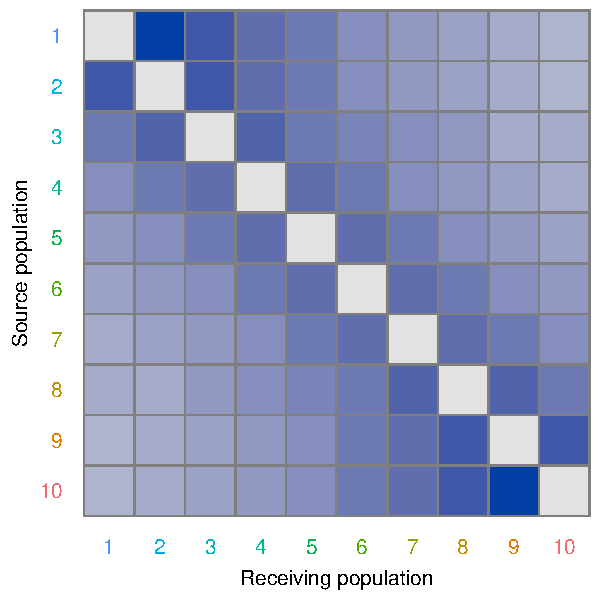
\includegraphics[width=3.5in]{metafolio/stray-matrix}
\caption[An example straying matrix.]{An example straying matrix. The rows and columns represent different
populations (indicated by population number). Dark blue indicates a high rate
of straying and light blue indicates a low rate of straying.}
\label{f:stray}
\end{figure}

\clearpage

%\textsc{Appendix D.} Sensitivity illustration with alternative parameter
%values. \renewcommand{\thefigure}{D\arabic{figure}}
%\setcounter{figure}{0}

\begin{figure}[htbp]
\centering
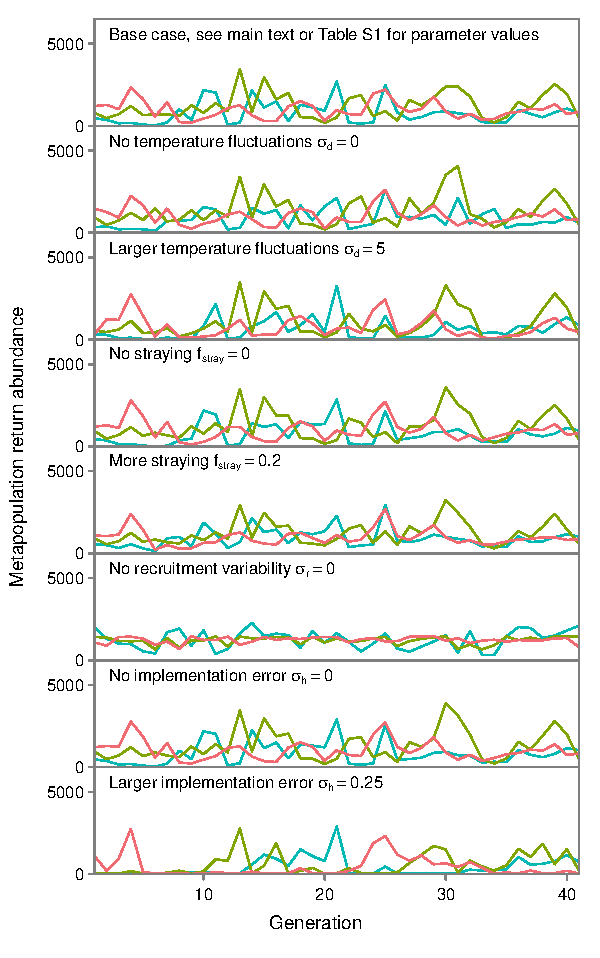
\includegraphics[width=3.5in]{metafolio/plot-various-options-ts-3pops}
\caption[The impact of increasing or decreasing various parameter values on
metapopulation return abundance.]{The impact of increasing or decreasing various parameter values on
metapopulation return abundance. The different coloured lines represent three
example salmon populations. The base case represents the base-case values for
the short-term environmental fluctuation scenario.}
\label{f:eg-sens}
\end{figure}

\clearpage

%\textsc{Appendix E.} An illustration of the correlation between
%populations. \renewcommand{\thefigure}{E\arabic{figure}}
%\setcounter{figure}{0}

\begin{figure}[htbp]
\centering
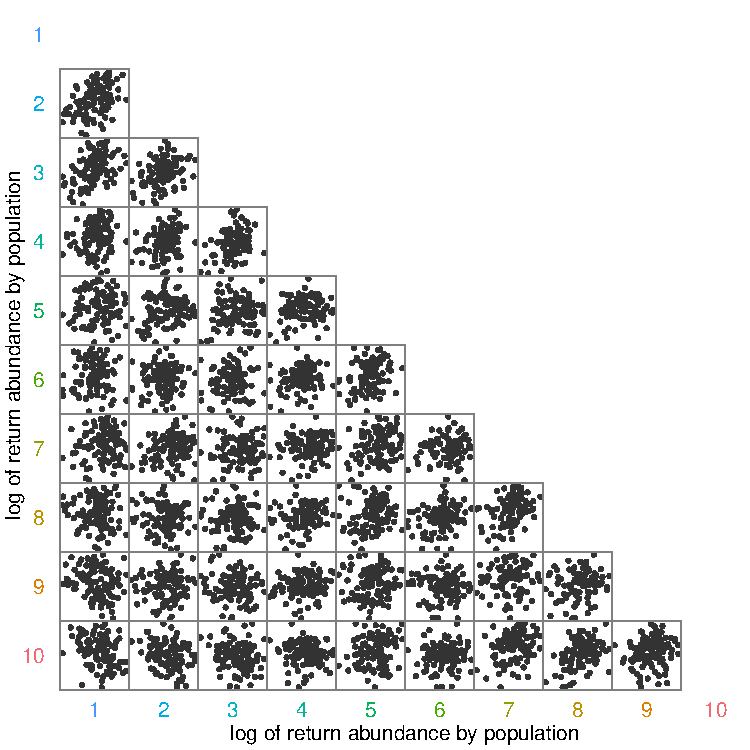
\includegraphics[width=4.5in]{metafolio/example-return-correlations}
\caption[A comparison of the log(returns) between populations.]{A comparison of the log(returns) between populations. The
subpopulation IDs are coloured from warm tolerant (warm colours) to cool
tolerant (cool colours). Note how populations 1 and 10 have asynchronous
returns whereas populations with more similar thermal-tolerance curves (say
populations 9 and 10) have more synchronous dynamics. Populations with
thermal tolerance curves in the middle (e.g. population 6) are less
correlated with other populations. Their population dynamics end up primarily
driven by demographic stochasticity and less so by temperature-induced
systematic changes in productivity.}
\label{f:ret-corr}
\end{figure}

\clearpage

%\textsc{Appendix F.} Example simulated time series from alternative
%conservation scenarios.

\begin{figure}[htbp]
\centering
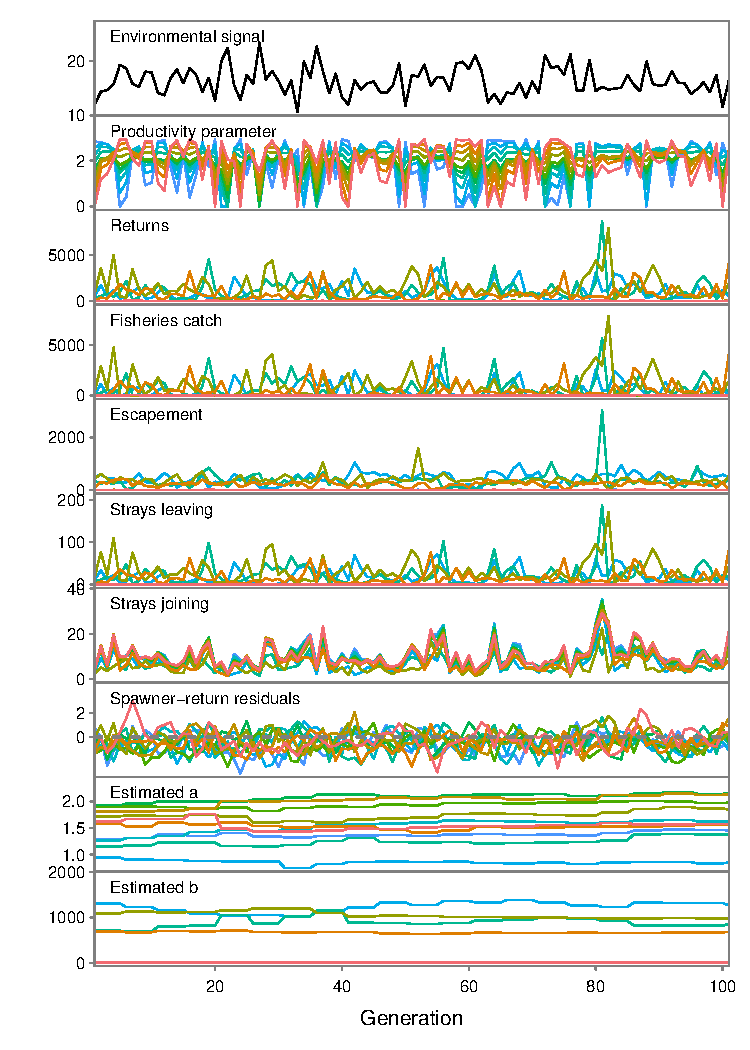
\includegraphics[width=4.3in]{metafolio/spatial-arma-sim-full-colour}
\caption[Conserving a \textbf{full range} of response diversity (spatial
conservation strategy) with \textbf{short-term} environmental fluctuations.]{Conserving a \textbf{full range} of response diversity (spatial
conservation strategy) with \textbf{short-term} environmental fluctuations. This is the same as Fig.~3 but in colour.}
\label{f:eg-sp-arma-full}
\end{figure}

\clearpage

\begin{figure}[htbp]
\centering
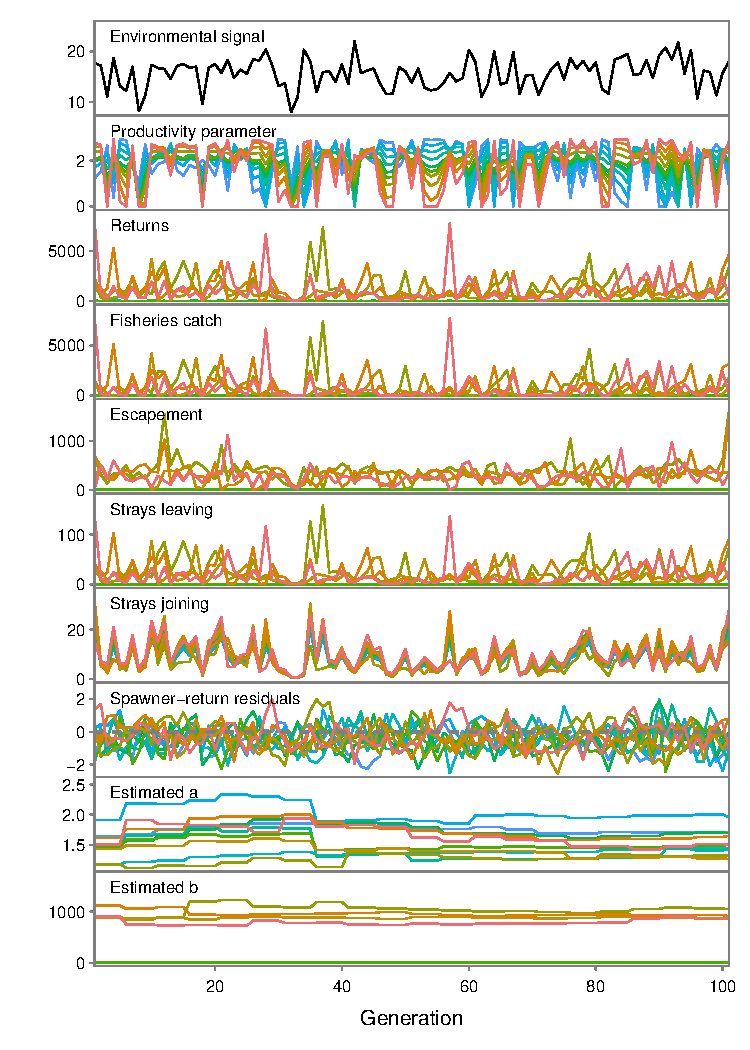
\includegraphics[width=4.3in]{metafolio/spatial-arma-sim-onehalf}
\caption{Conserving \textbf{one half} of response diversity (spatial
conservation strategy) with \textbf{short-term} environmental fluctuations.}
\label{f:eg-sp-arma-half}
\end{figure}

\clearpage

\begin{figure}[htbp]
\centering
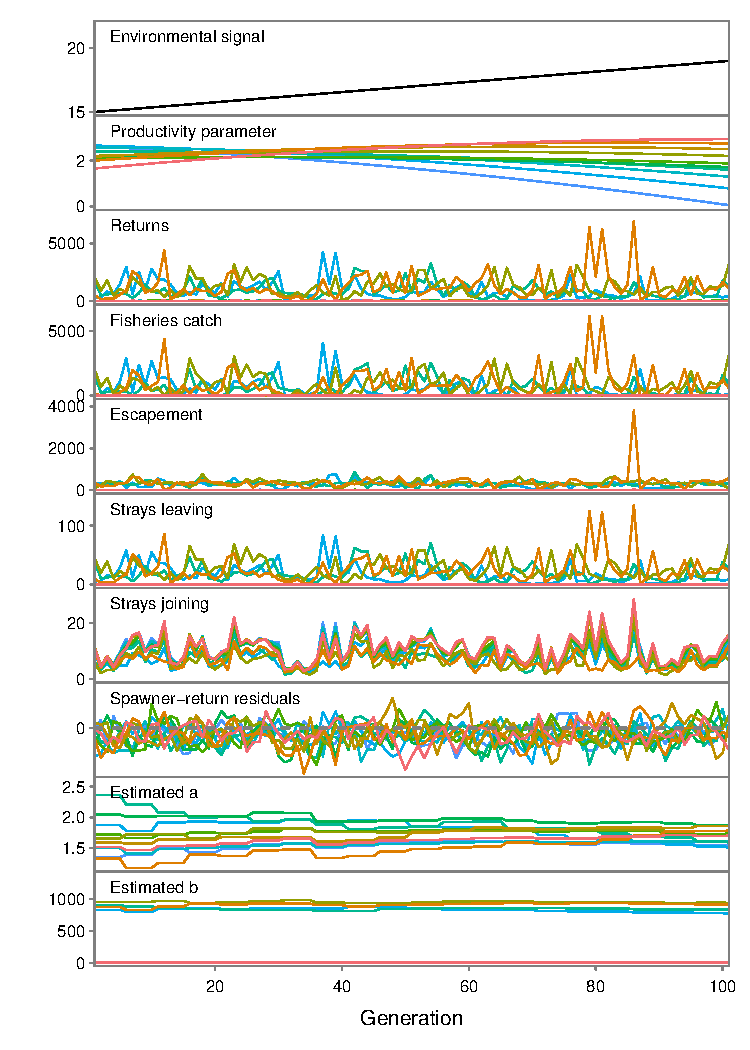
\includegraphics[width=4.3in]{metafolio/spatial-linear-sim-full}
\caption{Conserving a \textbf{full range} of response diversity (spatial
conservation strategy) with \textbf{long-term} environmental change.}
\label{f:eg-sp-linear-full}
\end{figure}

\clearpage

\begin{figure}[htbp]
\centering
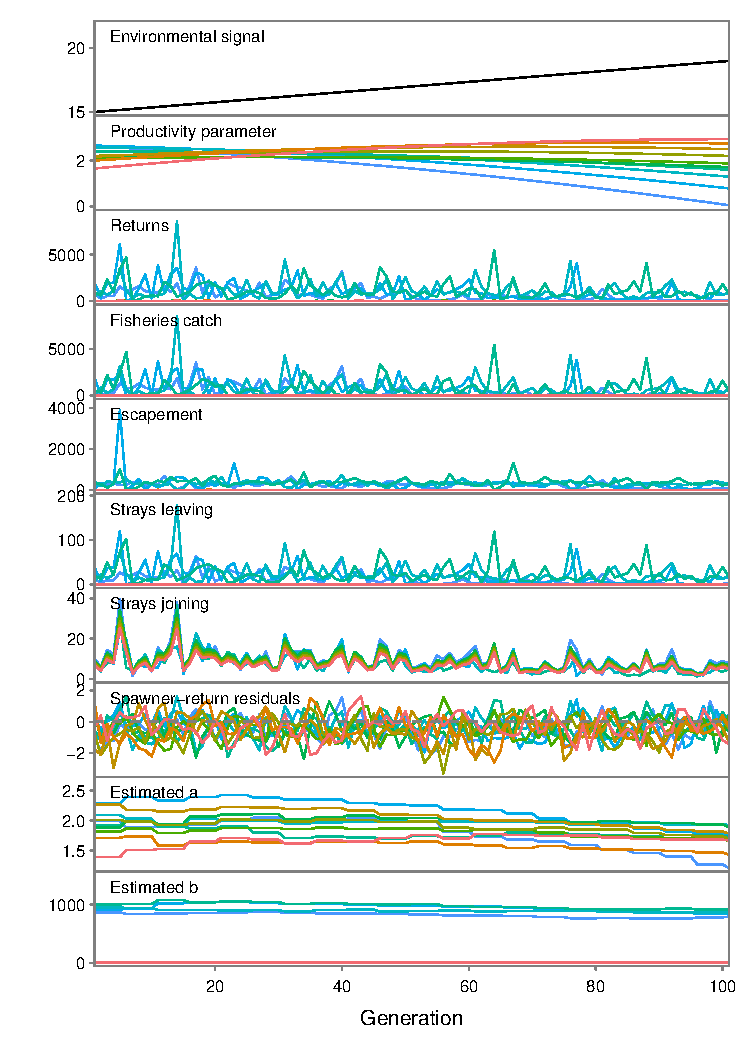
\includegraphics[width=4.3in]{metafolio/spatial-linear-sim-onehalf}
\caption{Conserving \textbf{one half} of response diversity (spatial
conservation strategy) with \textbf{long-term} environmental change.}
\label{f:eg-sp-linear-half}
\end{figure}

\clearpage

\begin{figure}[htbp]
\centering
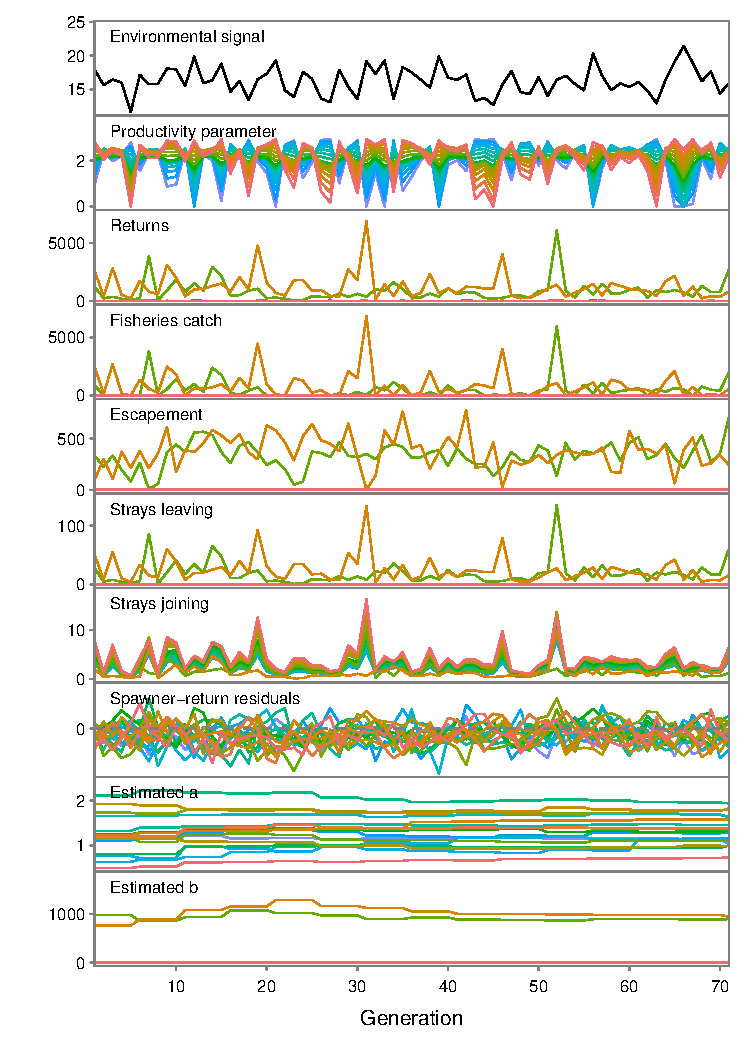
\includegraphics[width=4.3in]{metafolio/n-arma-sim-2}
\caption{\textbf{Two populations} conserved with random response diversity and
\textbf{short-term} environmental fluctuations.}
\label{f:eg-n-arma-two}
\end{figure}

\clearpage

\begin{figure}[htbp]
\centering
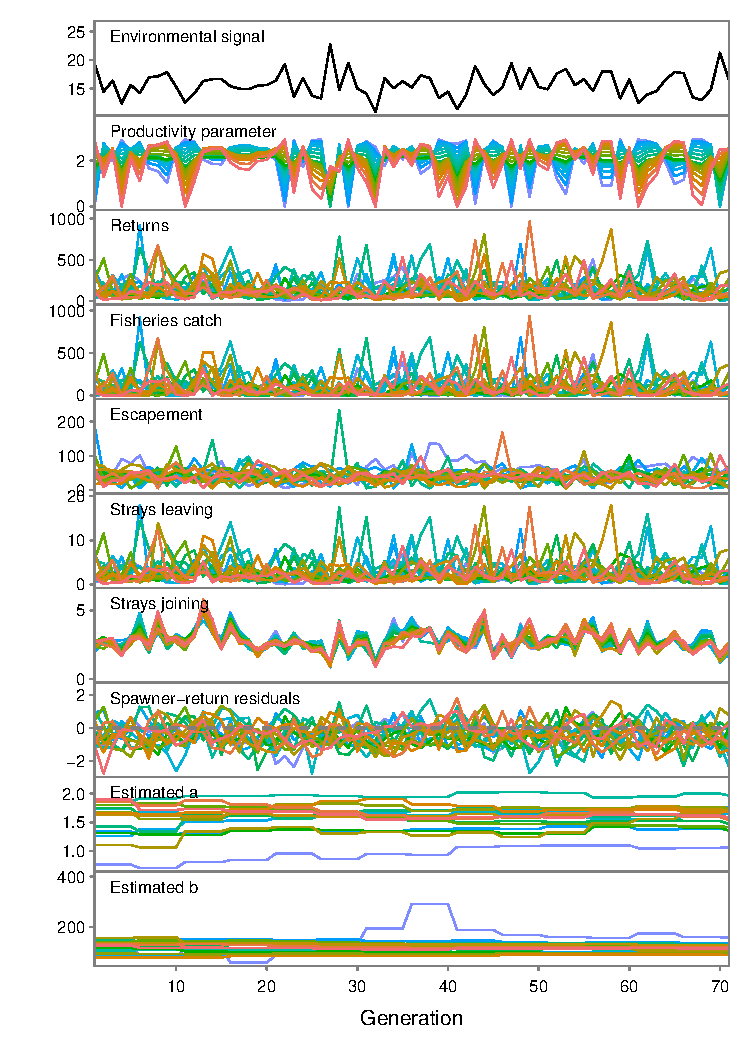
\includegraphics[width=4.3in]{metafolio/n-arma-sim-16}
\caption{\textbf{Sixteen populations} conserved with random response diversity
and \textbf{short-term} environmental fluctuations.}
\label{f:eg-n-arma-sixteen}
\end{figure}

\clearpage

\begin{figure}[htbp]
\centering
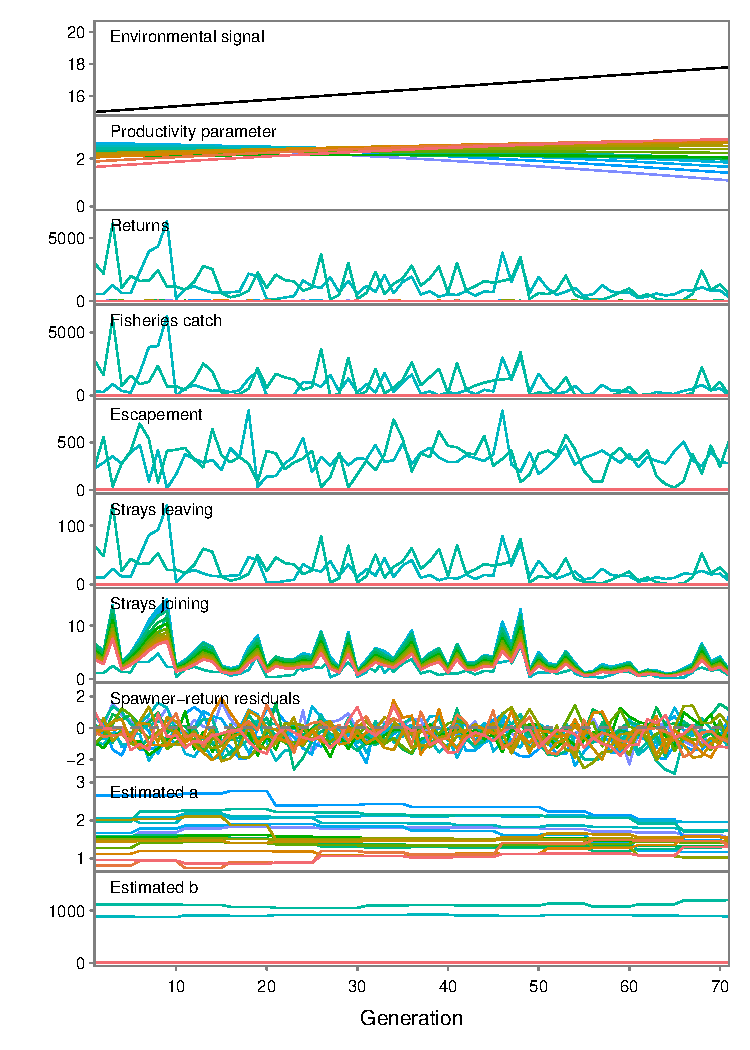
\includegraphics[width=4.3in]{metafolio/n-linear-sim-2}
\caption{\textbf{Two populations} conserved with random response diversity and
\textbf{long-term} environmental change.}
\label{f:eg-n-linear-two}
\end{figure}

\clearpage

\begin{figure}[htbp]
\centering
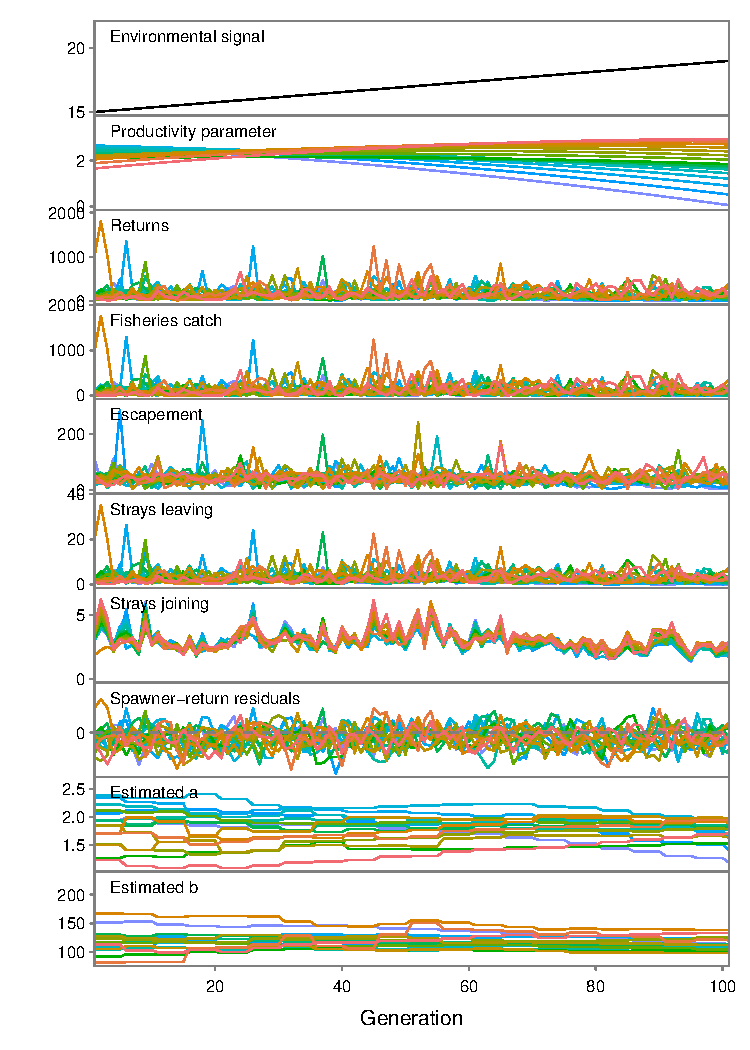
\includegraphics[width=4.3in]{metafolio/n-linear-sim-16}
\caption{\textbf{Sixteen populations} conserved with random response diversity
and \textbf{long-term} environmental change.}
\label{f:eg-n-linear-sixteen}
\end{figure}

\clearpage

\begin{figure}[htbp]
\centering
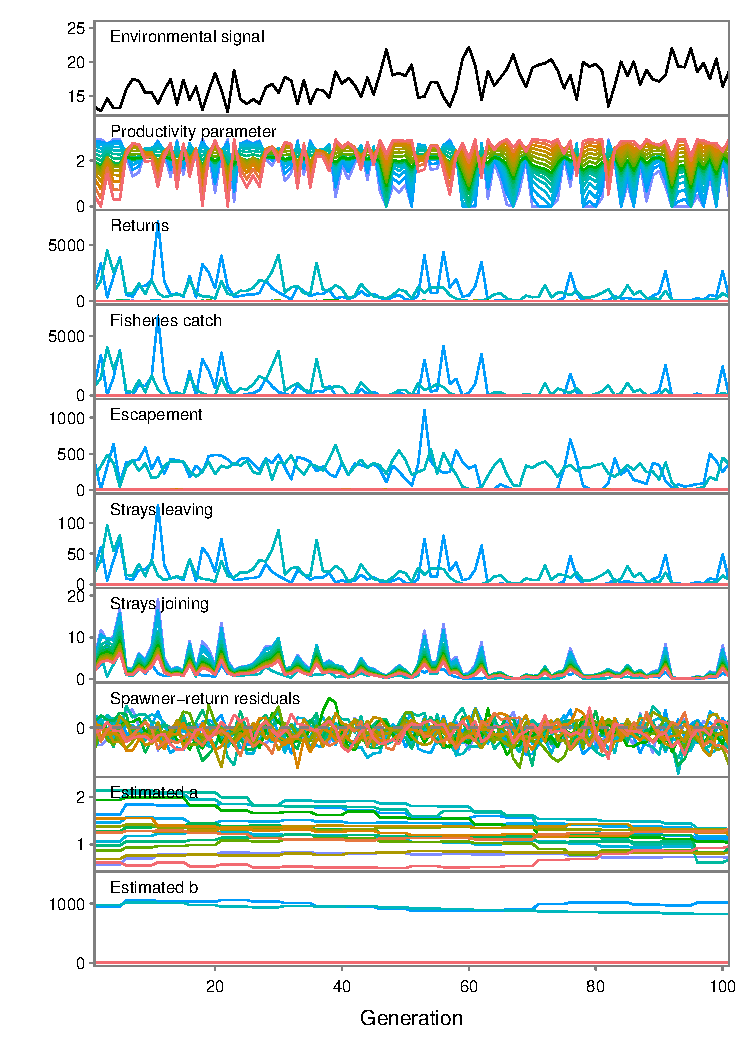
\includegraphics[width=4.3in]{metafolio/n-linear-arma-sim-2-squeeze}
\caption{\textbf{Two populations} conserved with random response diversity
and \textbf{long-term declining stream flow}.}
\label{f:eg-n-squeeze-two}
\end{figure}

\clearpage

\begin{figure}[htbp]
\centering
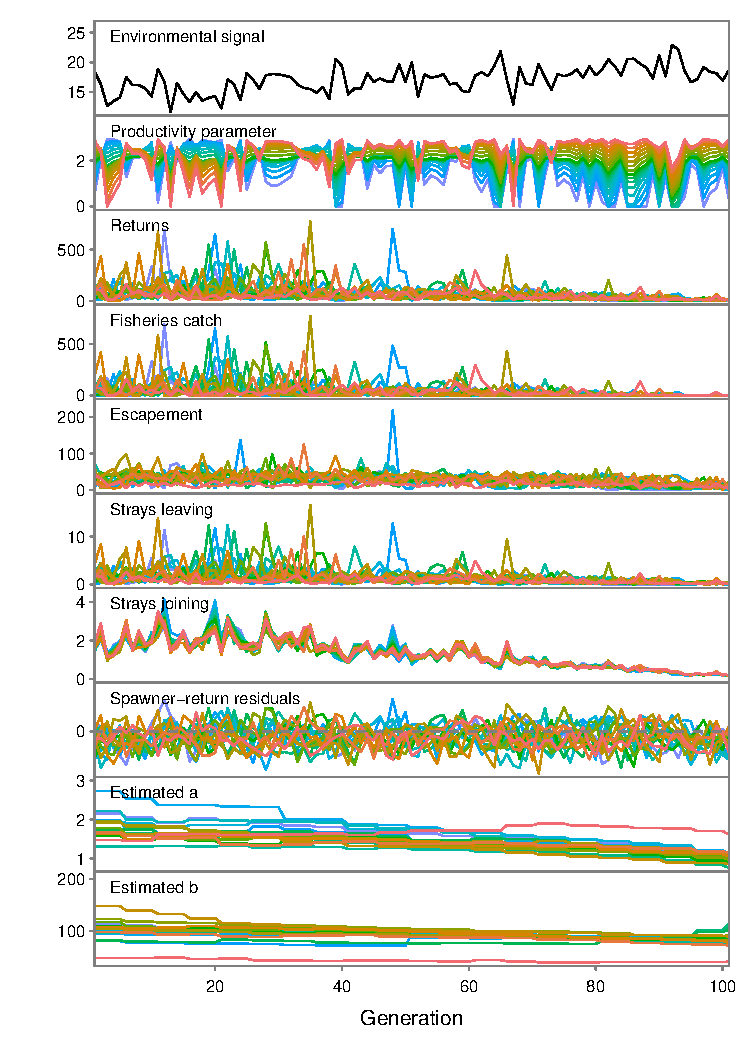
\includegraphics[width=4.3in]{metafolio/n-linear-arma-sim-16-squeeze}
\caption{\textbf{Sixteen populations} conserved with random response diversity
and \textbf{long-term declining stream flow}.}
\label{f:eg-n-squeeze-twelve}
\end{figure}

\end{appendices}

\newcommand{\basePriorMean}{102}
\newcommand{\basePriorMedian}{71}
\newcommand{\basePriorProbHeavy}{7.7}
\newcommand{\medianTimeSteps}{26}
\newcommand{\meanTimeSteps}{30.2}
\newcommand{\minTimeSteps}{20}
\newcommand{\maxTimeSteps}{117}
\newcommand{\birdN}{191}
\newcommand{\insectsN}{182}
\newcommand{\mammalsN}{125}
\newcommand{\fishN}{108}
\newcommand{\birdNH}{14}
\newcommand{\insectsNH}{5}
\newcommand{\mammalsNH}{6}
\newcommand{\fishNH}{0}
\newcommand{\birdPH}{7}
\newcommand{\insectsPH}{3}
\newcommand{\mammalsPH}{5}
\newcommand{\fishPH}{0}
\newcommand{\NOrdersHeavy}{15}
\newcommand{\POrdersHeavy}{38}
\newcommand{\baseFiftyObsFiftySwitch}{8}
\newcommand{\baseSeventyFiveObsFiftySwitch}{2}
\newcommand{\totalHeavyFifty}{26}
\newcommand{\totalHeavySeventyFive}{17}
\newcommand{\baseFiftyObsFiftySwitchPerc}{31}
\newcommand{\baseSeventyFiveObsFiftySwitchPerc}{8}
\newcommand{\baseNuTenObsTenSwitch}{8}
\newcommand{\baseNuTen}{26}
\newcommand{\baseNuFiveObsTenSwitch}{2}
\newcommand{\pHeavyNThirty}{0.13}
\newcommand{\pHeavyNSixty}{0.20}
\newcommand{\pIncHeavyNThirtyNSixty}{1.6}
\newcommand{\obsErrorNuFivePerc}{65}
\newcommand{\modelsNoConvergeAROne}{75}
\newcommand{\modelsNoConvergeAROneHeavyBase}{1}
\newcommand{\percImputedPops}{17}
\newcommand{\percImputedPoints}{0.7}
\newcommand{\nuCoefPopN}{606}
\newcommand{\AvesRangePerc}{4--8}
\newcommand{\InsectaRangePerc}{2--3}
\newcommand{\MammaliaRangePerc}{4--6}
\newcommand{\OsteichthyesRangePerc}{0}
\newcommand{\overallMinPerc}{3}
\newcommand{\overallMaxPerc}{5}
\newcommand{\NPops}{609}
\newcommand{\NOrders}{39}
\newcommand{\NClasses}{7}
\newcommand{\interpPointsPerc}{1}
\newcommand{\nBSUp}{8}
\newcommand{\nBSDown}{52}
\newcommand{\ratioBSDownToUp}{6.5}
\newcommand{\percBSDown}{87}
 % R output
\chapter[Ecological black swans]{Evidence for black-swan events in animal
  populations\footnotemark[3]}

\footnotetext[3]{T.A. Branch, A.B. Cooper, and N.K. Dulvy are co-authors on this
chapter, which is in preparation for submission to a journal.}
%!TEX root = anderson-etal-blackswan-timeseries.tex

\section{Abstract}

Black swans are statistically improbable events that nonetheless occur---often
with profound consequences. While extremes in the physical environment, such
as monsoons and heat waves, are widely studied and increasing in magnitude and
frequency, it remains unclear the extent to which ecological populations
buffer or suffer from such extremes. Here, we estimate the degree of
heavy-tailedness (presence of black swans) in ecological process noise by
applying a probability model to \NPops~time series from around the world
across \NOrders~taxonomic orders and seven classes. We find strong evidence of
black swans, but they are rare, occurring in
\overallMinPerc--\overallMaxPerc\% of populations: most frequently for birds
(\AvesRangePerc\%) followed by mammals (\MammaliaRangePerc\%) and insects
(\InsectaRangePerc\%). Black swans were predominantly (\percBSDown \%)
downward events and were not explained by any life-history covariates, but
tended to be driven by external perturbations such as climate, severe winters,
predator or parasite cycles, and the combined effects of multiple factors.
Extreme events were more frequently detected for populations with longer time
series and lower levels of process noise; for shorter and noisier time series,
our simulations suggested black-swan dynamics are often not identifiable as
such. The presence of black swans in population dynamics highlights the
importance of developing robust conservation and management
strategies---particularly as the frequency and magnitude of climate extremes
increase over the next century.

\section{Introduction}

Black swans are unexpected extreme events with potentially dramatic
consequences \citep{taleb2007,sornette2009}. One of the most striking black
swans in ecology is the asteroid collision that may have marked the
end-Cretaceous mass extinction 65 million years ago
\citep{alvarez1980,harnik2012}. Today, climate extremes, in concert with
shifts in mean temperature, are expected to cause the greatest ecological and
societal damage \citep{ipcc2012}. But, while extremes in the physical
environment such as wave height, storm severity, and temperature are frequent
events \citep{gaines1993,katz2005}, it remains unclear the extent to which
ecological systems buffer or suffer from black swans \citep{nunez2012}.

There is compelling anecdotal evidence for ecological black swans, but
systematic evidence across taxa has been elusive. A survey of ecologists
indicated that surprising outcomes of field experiments are far more common
than we assume \citep{doak2008}, and events such as the global invasion of
Argentine ants and the mutation of viruses to infect new hosts could be
considered black swans \citep{nunez2012}. In fact, anecdotes of population
catastrophes are numerous and catastrophes may be the most important element
affecting population persistence \citep{mangel1994}. For marine mammal
populations, we have compelling evidence of catastrophes \citep{gerber2001,
  ward2007}, and recently, time-series of marine microbe abundance
\citep{segura2013} and time to extinction for experimental waterflea
populations \citep{drake2014} have been found to follow heavier tailed
distributions than the normal. Despite these examples, as far as we can tell
there have been two systematic surveys for ecological black swans: one with
North American breeding birds and the other with the Global Population
Dynamics Database, which uncovered little clear evidence for them
\citep{keitt1998,allen2001,halley2002}. Nevertheless there are methodological
challenges to their detection \citep{allen2001,ward2007}.

There are two key reasons why we may find little evidence of ecological black
swans. First, they might not exist in higher taxa. Indeed, the majority of
model fitting and risk forecasting assumes that population dynamics are normal
tailed on a log scale \citep[e.g.][]{brook2006a,dennis2006,knape2012}.
Alternatively, black-swan dynamics might exist, but our ability to detect
them requires further development of statistical tools. One such tool is the
generalized extreme value distribution, which has been applied to
environmental data \citep[e.g.][]{katz2005}. This distribution describes the
most extreme event per time interval (e.g.~heaviest rainfall per year), but
requires time series that are sufficiently long to be condensed into time
intervals. Another statistical tool involves fitting a catastrophic mixture
distribution in a state space model to quantify the probability that
population events are extreme, although this is also data intensive
\citep{ward2007}. A third tool is to compare the support for fits of thin- and
heavy-tailed distributions \citep{halley2002}, but this analysis did not
quantify the probability of black swans or allow for population dynamics.

Here, we assess the frequency and magnitude of black-swan dynamics across
\NPops\ populations from a wide array of taxonomic groups---mostly birds,
mammals, insects, and fishes. We then identify characteristics of time series
or intrinsic life-history characteristics that are associated with the
detection of black-swan events and attempt to verify known causes. To
accomplish this, we develop a framework for identifying heavy-tailed process
noise in population dynamics, i.e.\ whether the largest stochastic jumps in
abundance from one time step to the next are more extreme than typically seen
with a log-normal distribution. Our framework allows for a range of population
dynamic models, can incorporate observation uncertainty, and can be easily
applied to abundance time series.

\section{Methods}

To obtain estimates of the probability and magnitude of black-swan events, we
fit population dynamic models to abundance time series from around the world.
For each population, we estimated the shape of the process noise tails by
measuring the degrees of freedom ($\nu$) of a Student t-distribution.

\subsection{Time-series data}

We selected abundance time series from the Global Population Dynamics Database
(GPDD; \citeauthor{gpdd2010} \citeyear{gpdd2010}), which contains nearly 5000
time series of abundance from $\sim$1000 species and $\sim$100 taxonomic
orders. We filtered the data (Supporting materials) to remove populations
from less reliable data sources, and those without sufficient data for our
models, and then interpolated some missing values
\citep[\textit{sensu}][]{brook2006a}. Our interpolation affected only
$\sim$\interpPointsPerc \% of the final data points (Supporting materials~Table~\ref{tab:stats})
and none of the data points that were later considered black-swan events. Our
final dataset contained \NPops~populations across \NOrders~taxonomic orders
and seven taxonomic classes, with a median of \medianTimeSteps~time steps
(range of \minTimeSteps--\maxTimeSteps) (Supporting materials Table~\ref{tab:stats},
Fig.~\ref{fig:all-ts}).

\subsection{Population models}

Our main analysis focuses on the commonly applied Gompertz population dynamics
model \citep[e.g.][]{knape2012,dennis2014,connors2014}. The Gompertz model
represents population growth as a linear function in $\log$ space. If we let
$x_t$ represent the $\log$ abundance ($N$) at time $t$, we can represent the
Gompertz model as:
\begin{align*}
x_t &= \lambda + b x_{t-1} + \epsilon_t\\
\epsilon_t &\sim \mathrm{Student\mhyphen t}(\nu, 0, \sigma).
\end{align*}
The growth parameter $\lambda$ represents the expected growth rate if $N_t =
1$. The model is density independent if $b = 1$, maximally density dependent
if $b = 0$, and inversely density dependent if $b < 0$. Usually, the process
noise $\epsilon_t$ is modelled as normally distributed, but in our paper we
assume it is drawn from a t distribution with scale parameter $\sigma$ and
degrees of freedom $\nu$. In previous analyses of the GPDD, the Gompertz was
most often identified as the most parsimonious population model fit to these
data \citep{brook2006}.

By allowing the process noise to be drawn from a Student-t distribution we can
estimate the degree to which the process deviations have heavy tails and are
thereof evidence of black-swan events (Fig.~\ref{fig:didactic}a, b). For
example, at $\nu = 2$, the probability of drawing a value more than five
standard deviations below the mean is $0.02$, whereas the probability of
drawing such a value from a normal distribution is tiny ($2.9\cdot10^{-7}$).
As the value of $\nu$ approaches infinity, the distribution approaches the
normal distribution (Fig.~\ref{fig:didactic}a, b). While, across populations,
the extreme process deviations might tend to be more frequently upwards or
downwards events, a small random sample from a heavy-tailed distribution can
have many outliers on one side and appear asymmetric \citep{gelman2013a}.
Therefore, fitting a symmetric t distribution is appropriate for the
relatively short population time series in our dataset and is agnostic towards
the detection of upwards or downwards black swans.

\begin{figure}[htbp]
\begin{center}
\includegraphics[width=\textwidth]{blackswans/analysis/t-nu-eg2.pdf}
\caption[An illustration of fitting population dynamic models that allow for heavy
tails, represented by the Student-t degrees of freedom parameter $\nu$.]{
An illustration of fitting population dynamic models that allow for heavy
tails, represented by the Student-t degrees of freedom parameter $\nu$. (a, b)
The probability density for t distributions with a scale parameter of 1 and
different values of $\nu$. Small values of $\nu$ create heavy tails. As $\nu$
approaches infinity the distribution approaches the normal distribution. For
example, at $\nu = 2$, the probability of drawing a value more than five
standard deviations below the mean is $0.02$, whereas the probability of drawing
such a value from a normal distribution is nearly zero ($2.9\cdot10^{-7}$).
(c--e) Simulated population dynamics from a Gompertz model with process noise
drawn from t distributions with three different values of $\nu$. Coloured dots
in panels c and d represent jumps with less than a 1 in 1000 chance of
occurring in a normal distribution. (f--h) Estimates of $\nu$ from models fit
to the times series in panels c--e. Shown are the posterior samples
(histograms), median and interquartile range of the posterior (IQR) (dots and
line segments), and the exponential prior on $\nu$ (dashed lines). Colour
shading behind panels f--h illustrates the region of heavy tails.
}
\label{fig:didactic}
\end{center}
\end{figure}

We fit all models in a Bayesian framework using Stan \citep{stan-manual2014}
via the R computing environment \citep{r2014}. Stan samples from the posterior
distribution with an adaptive version of Hamiltonian Markov chain Monte Carlo
called the No-U-Turn Sampler and generally obtains less correlated samples
than algorithms such as the Gibbs sampler \citep{hoffman2014}. We tested to
ensure that the chains had sufficiently converged and that the sampler had
obtained sufficient independent samples from the posterior ($\widehat{R} <
1.05$, $n_\mathrm{eff} > 200$; Supporting materials).

We chose weakly informative priors to incorporate our understanding of
plausible population dynamics (\citeauthor{gelman2014} \citeyear{gelman2014};
Figs~\ref{fig:didactic}f--h, \ref{fig:priors}). For $\nu$, we chose an
exponential prior with rate parameter of $0.01$ truncated at values above
two---a slightly less informative prior than suggested by
\citet{fernandez1998}. This prior gives only a \basePriorProbHeavy \%
probability that $\nu < 10$ but constrains the sampling sufficiently to avoid
wandering off towards infinity. In any case, for $\nu > 20$ the t distribution
is almost indistinguishable from the normal distribution
(Fig.~\ref{fig:didactic}). Based on the shape of the t distribution, we chose
the probability that $\nu < 10$, Pr($\nu < 10$), to define the probability of
heavy-tailed dynamics. When categorizing a population as heavy or normal tailed,
we used a threshold of 0.5 probability.

We fit alternative population models to test if four key phenomena
systematically changed our conclusions. Autocorrelation has been suggested as
a reason for increased observed variability of abundance time series through
time, which could create apparent heavy tails \citep{inchausti2002};
therefore, we fit a model that included serial correlation in the residuals.
Additionally, previous work has modelled abundance or growth rates without
accounting for density dependence \citep{halley2002,segura2013}; therefore, we
fit a simpler model in which we assumed density independence. Third,
observation error could bias parameter estimates \citep{knape2012} or mask our
ability to detect heavy tails \citep{ward2007}; therefore, we fit a model
where we allowed for a fixed quantity of observation error ($0.2$ standard
deviations on a log scale). Finally, the Gompertz model assumes that
population growth rate declines linearly with log abundance. Therefore, we
also fit an alternative model, the Ricker-logistic model, which assumes that
population growth rate declines linearly with abundance itself (Supporting
materials).

In addition to alternative population models, we investigated the sensitivity
of our results to weaker and stronger priors (exponential rate parameter $=
0.005, 0.02$; Supporting materials Fig.~\ref{fig:priors}, Supporting materials). We used
simulated data to test how easily we could detect $\nu$ given different sample
sizes and to ensure we could recover unbiased parameter estimates from the
Gompertz model (Supporting materials).


\subsection{Covariates of population dynamic black swans}

We investigated possible covariates of heavy-tailed population dynamics
visually and through multilevel modelling. We plotted characteristics of the
time series ($\sigma$, $\lambda$, $b$, and time-series length) along with two
life-history characteristics (body length and maximum lifespan obtained from
\citet{brook2006a}) against our estimated probability of heavy tails, Pr$(\nu <
10)$. We formally investigated these relationships by fitting beta
regression multilevel models \citep{ferrari2004}. The beta probability
distribution can represent continuous response data that range between zero
and one; we fit our models with a logit link as is common for beta and logistic
regression \citep{ferrari2004}. We incorporated standard deviations around the
means for covariates that were derived from Gompertz model parameter
estimates. To account for broad patterns of phylogenetic relatedness, we
allowed for hierarchical intercepts at the taxonomic class, order, and species
level (Supporting materials). We fit our model in Stan with weakly
informative priors on the coefficients \citep{gelman2008d} and variance
parameters (\citeauthor{gelman2006c} \citeyear{gelman2006c};
\citeauthor{gelman2014} \citeyear{gelman2014}; Supporting materials).

Finally, we investigated a sample of populations that our method categorized as
having a high probability of heavy tails (Pr$(\nu < 10) > 0.5$). Where
possible, we found the documented causes of ecological black swans in the
primary data source cited in the GPDD or in other literature describing the
population.

\section{Results}

We found strong, but rare, evidence for black-swan population dynamics. By
defining black-swan dynamics as a greater than $0.5$ probability that $\nu <
10$, our main Gompertz model found evidence for heavy tails most frequently
for birds (\birdPH\%) followed by mammals (\mammalsPH\%), and insects
(\insectsPH\%) (Fig.~\ref{fig:nu-coefs}, Supporting materials Table~\ref{tab:causes-supp}). Black
swans were taxonomically widespread, occurring in \POrdersHeavy\% of taxonomic
orders. Accounting for time series length and partially pooling inference
across taxonomic class and order with a multilevel model (Supporting
materials), there was stronger evidence for black swans in insect
populations than is visually apparent in Fig.~\ref{fig:nu-coefs}---four of 10
orders with the highest median probability of heavy tails were insect
orders---however, there was considerable uncertainty in these estimates
(Fig.~\ref{fig:posteriors}a).

\begin{figure}[htbp]
\begin{center}
\includegraphics[width=0.44\textwidth]{blackswans/analysis/nu-coefs-2.pdf}

\caption[Estimates of population dynamics heavy-tailedness for \nuCoefPopN\
  populations of birds, mammals, insects, and fishes.]{Estimates of population dynamics heavy-tailedness for \nuCoefPopN\
  populations of birds, mammals, insects, and fishes. Small values of $\nu$
  approximately ($< 10$) suggest heavy-tailed black-swan dynamics; larger values of
  $\nu$ suggest approximately normal-tailed dynamics. Vertical points and line
  segments represent posterior medians and 50\% / 90\% credible intervals for
  individual populations. Inset plots show probability that $\nu < 10$
  (probability of heavy tails) for populations arranged by taxonomic order and
  sorted by decreasing mean Pr($\nu < 10$). Taxonomic orders with three or
  fewer populations in panel a are omitted for space. Red to yellow points
  highlight populations with a high to moderately high probability of
  heavy-tailed black-swan dynamics.}

\label{fig:nu-coefs}
\end{center}
\end{figure}

\begin{figure}[htbp]
\begin{center}
\includegraphics[width=0.45\textwidth]{blackswans/analysis/order-posteriors-covariates.pdf}

\caption[Posterior probability distributions from beta regression multilevel
  models.]{Posterior probability distributions from beta regression multilevel
  models. (a) Taxonomic-order-level posterior densities of Pr($\nu < 10$)
  (approximately the probability of heavy tails) after accounting for
  time-series length. Estimates are at the geometric mean of time series
  length across all the data (approximately 27 time steps). Colour shading
  refers to taxonomic class (yellow: fishes, green: insects, purple: birds,
  and red: mammals). Dotted vertical line in panel a indicates the
  Pr($\nu < 10$) from the prior distribution. (b) Main effect
  posterior densities for potential covariates of Pr($\nu < 10$). The beta
  regression models were fit on a logit scale with hierarchical intercepts for
  taxonomic class, taxonomic order, and species. All covariates were
  standardized by subtracting their mean and dividing by twice their standard
  deviation. In both panels, short vertical line segments within the density
  polygons indicate median posterior estimates.}

\label{fig:posteriors}
\end{center}
\end{figure}


The majority of our heavy-tailed estimates were robust to alternative
population models, observation error, and choice of priors. Our conclusions
were not systematically altered when we included an autocorrelation structure
in the residuals, modelled population growth rates without density dependence,
or modelled the population dynamics as Ricker-logistic (Supporting materials Fig.~\ref{fig:alt}).
However, setting observation error standard deviation to $0.2$ increased the
median estimate of $\nu$ from $<10$ to $\ge 10$ in $\baseNuTenObsTenSwitch$ of
$\baseNuTen$ populations, although the majority of $\nu$ estimates remained
qualitatively similar (Supporting materials Fig.~\ref{fig:alt}). The strength of the prior on $\nu$
had little influence on estimates of black-swan dynamics
(Supporting materials~Fig.~\ref{fig:alt-priors}). Our simulation testing shows that, if anything,
our models underpredict the true magnitude and probability of heavy tailed
events---especially given the length of the time series in the GPDD
(Supporting materials Figs~\ref{fig:sim-nu}, \ref{fig:sim-prob}).

Across populations, the probability of observing black-swan dynamics was
positively related to time-series length and negatively related to magnitude
of process noise ($\sigma$) but not clearly related to population growth rate
($\lambda$), density dependence ($b$), or maximum lifespan
(Figs~\ref{fig:posteriors}b, \ref{fig:correlates}). Longer time-series length
was the strongest covariate of observing black-swan dynamics. For instance,
the expected probability density below $\nu = 10$ was about \pIncHeavyNThirtyNSixty~times
greater for a population with 60 time steps compared
to one with 30 time steps. However, the absolute change in probability with
increased time series length was small ($\pHeavyNSixty$ vs.\ $\pHeavyNThirty$
in the previous example, Fig.~\ref{fig:correlates}).

\begin{figure}[htbp]
\begin{center}
\includegraphics[width=0.9\textwidth]{blackswans/analysis/correlates-p10.pdf}

\caption[Potential covariates of heavy-tailed population dynamics.]{Potential covariates of heavy-tailed population dynamics (indicated
  by a high probability that $\nu < 10$). Shown are (a--c) parameters from the
  Gompertz heavy-tailed population model ($\sigma$, $\lambda$, $b$), (b)
  number of time steps, (c) body length, and (d) lifespan. For the Gompertz
  parameters, $\sigma$ refers to the scale parameter of the Student-t
  process-noise distribution, $\lambda$ refers to the expected log abundance
  at the next time step at an abundance of one, $b$ refers to the density
  dependence parameter ($1$ is maximally density independent, $0$ is maximally
  density dependent, and $<0$ is inversely density dependent). Circles
  representing a few sharks, crustaceans, and gastropods are filled in white.
  Median and 90\% credible interval posterior predictions of a beta regression
  multilevel model are shown in panels a and d where there was a high
  probability the slope coefficient was different from zero
  (Fig.~\ref{fig:posteriors}b).}

\label{fig:correlates}
\end{center}
\end{figure}



\LTcapwidth=\textwidth
\bibpunct{}{}{;}{a}{}{;}

\begin{small}
\begin{longtable}{>{\RaggedRight}m{2.0cm}>{\RaggedRight}p{3.0cm}>{\RaggedRight}p{7.0cm}>{\RaggedRight}p{2.0cm}}

\caption[Example population dynamic black swans from the Global Population
  Dynamics Database and a description of their causes.]{Example population dynamic black swans from the Global Population
  Dynamics Database and a description of their causes. Red and blue dots
  indicate downward and upward events that have a $10 \cdot 10^{-4}$ probability or less of
  occurring if the population dynamics were explained by a Gompertz model
  with normally distributed process noise. These populations are
  a sample from the heavy-tailed populations we could verify
  (Table~\ref{tab:causes-supp}).}\\

\toprule
Time series (log scale) & Population & Black swan description & Reference \\
\midrule

\includegraphics[width=2cm]{blackswans/analysis/sparks/6528} &
Shag,
\textit{Phalacrocorax aristotelis},
UK &
Shortage of nest sites reduced productivity; red-tide event in 1968 caused
extreme mortality; no longer a nest shortage; population rapidly increased &
\citep{potts1980}\\

\includegraphics[width=2cm]{blackswans/analysis/sparks/10007} &
Water vole,
\textit{Arvicola terrestris},
UK &
Short-term population cycles from predator interactions combined with long-term
environmental cycle caused sharp downswing  &
\citep{saucy1994}\\

\includegraphics[width=2cm]{blackswans/analysis/sparks/7115} &
Fur seal,
\textit{Arctocephalus pusillus},
South Africa &
Strong decreases in harvesting, loss of predators, and diamond mining
regulations reducing human traffic caused sharp upswings  &
\citep{shaughnessy1982}\\

\includegraphics[width=2cm]{blackswans/analysis/sparks/10113} &
Willow grouse,
\textit{Lagopus lagopus},
UK &
Parasite and predation effects interacted to cause low years  &
\citep{dobson1995}\\

\includegraphics[width=2cm]{blackswans/analysis/sparks/10162} &
Red grouse,
\textit{Lagopus lagopus scoticus},
UK &
Good environmental conditions produced high numbers and vulnerable populations;
bad conditions and overcrowding combined to create crashes  &
\citep{mackenzie1952}\\

\includegraphics[width=2cm]{blackswans/analysis/sparks/1235} &
Wren,
\textit{Troglodytes troglodytes},
UK &
Severe winters where food was buried under snow caused population crash &
\citep{newton1998} \\

\includegraphics[width=2cm]{blackswans/analysis/sparks/20579} &
Grey heron,
\textit{Ardea cinerea},
UK &
Severe winters in 1929, 1940--1942, and 1962--1963; 1963 event so severe that
recovery took three times longer than expected &
\citep{stafford1971} \\

%\includegraphics[width=2cm]{blackswans/analysis/sparks/20580} &
%Chamois, \textit{Rupicapra rupicapra}, Switzerland &
% &
%\citep{brook2006a}\\

%\includegraphics[width=2cm]{blackswans/analysis/sparks/5019} &
%Barbary macaque,  &
% &
%REF\\

%\includegraphics[width=2cm]{blackswans/analysis/sparks/9675} &
%Carrot fly (\textit{Psila rosae}, Finland &
% &
%\citep{markkula1965}\\

%\includegraphics[width=2cm]{blackswans/analysis/sparks/10139} &
%Grey heron (\textit{Ardea cinerea}), UK &
% &
%\citep{stafford1971}\\

\bottomrule
\label{tab:sparks}
\end{longtable}
\end{small}

% reset citation style:
\bibpunct{(}{)}{;}{a}{}{;}


We examined all time series with published explanations of why the black-swan
events occurred (Table~\ref{tab:sparks} and Supporting materials~Table~\ref{tab:causes-supp}). The
majority of documented events (\percBSDown \%) were downward black swans and
involved a combination of multiple factors. For example, a synchronization of
environmental- and predation-mediated population cycles are thought to have
caused a downward black-swan event for a water vole (\textit{Arvicola
  terrestris}) population \citep{saucy1994}. Other black swans were the result
of a sequence of extreme climate events on their own. For instance, severe
winters in 1929, 1940--1942, and 1962--1963 were associated with black-swan
downswings in grey heron (\textit{Ardea cinerea}) abundance in the United
Kingdom \citep{stafford1971}. Our analysis finds that the last event was a
combination of two black-swan events in a row and it took the population three
times longer to recover than predicted \citep{stafford1971}. Downwards black
swans were sometimes followed by upwards black swans. For example, during a
period of population crowding and nest shortages, a population of European
shag cormorants (\textit{Phalacrocorax aristotelis}) on the Farne Islands,
United Kingdom, declined suddenly following a red tide event in 1968
\citep{potts1980}. This freed quality nest sites for first-time breeders,
productivity rapidly increased, and the population experienced a rapid upswing
in abundance \citep{potts1980}.


\section{Discussion}

We found strong evidence for black swans (heavy-tailed process noise) in
\overallMinPerc--\overallMaxPerc\% of ecological time series. Black swans were
usually (\percBSDown \%) downward events and were detected more frequently in
longer time series and in populations with a smaller magnitude of process
noise. Black swans were not associated with density dependence, population
growth rate, or lifespan. In verified cases, black-swan events were often a
result of the combination of extreme climate, predators and parasite cycles,
and strong changes in human pressures. Our empirical results, sensitivity
analyses, and simulation tests suggest that estimating the tail shape of
process noise is a viable method of detecting black-swan population dynamics
and if anything will underestimate the probability of black-swan events. The
presence of black swans highlights the importance of developing management
strategies that detect quickly, respond to, and are robust to extremes in
population dynamics---particularly as the frequency and magnitude of climatic
extremes increase over the next century \citep{easterling2000,ipcc2012}.

Our results clarify previous related analyses. An analysis with an older
version of the GPDD assessed the distribution of abundance time series but
focused on identifying if the log-normal distribution was the most frequently
parsimonious model \citep{halley2002}. For heavy-tailed distributions,
\citet{halley2002} fit the extremely heavy-tailed Cauchy distribution and the
four-parameter Levy stable distribution and found little information criteria
support for these distributions in longer time series. However, black-swan
events are by definition rare, and the majority of time series in the GPDD are
short for these purposes. Therefore, we would not expect to observe black
swans in a large proportion of populations. By quantifying the probability of
heavy-tails and allowing for non-stationary time series and density
dependence, our analysis allows for a more nuanced description of the evidence
of ecological black swans. In an earlier study, \citet{keitt1998} described
heavy (power law) tails in breeding bird population abundance. However, this
finding was challenged by \citet{allen2001}, who showed that mixing data
across species could falsely generate heavy tails.
%This rebuttal supports our
%use of the t distribution to represent heavy tails, since a t distribution can
%be represented by a mixture of normal distributions \citep[with the same mean
%and inverse-gamma-distributed variances,][]{gelman2014}.

We might expect to observe black-swan dynamics in ecological time series
because of unmodelled intrinsic properties of populations or extrinsic forces
acting on populations. Since a t-distribution can be formed by a mixture of
normal distributions \citep[with the same mean and inverse-gamma-distributed
variances,][]{gelman2014}, we could observe heavy tails if we miss some
underlying mixture of intrinsic processes \citep{allen2001}. That process
might be an aggregation of populations across space, or population diversity,
or an intrinsic change in population variability through time. Extrinsic
forces could also cause black-swan dynamics \citep[e.g.][]{nunez2012}. These
forces could be extreme themselves. For example, extreme climate, predation
from (or competition with) other species experiencing black swans, or sharp
changes in human pressure such hunting, fishing, or habitat destruction might
cause black swans. Alternatively, the synchrony of multiple ``normal''
extrinsic forces could give rise to black-swan ecological dynamics. This could
occur with a synergistic interaction \citep[e.g.][]{kirby2009} or even if
non-synergistic forces experience a rare alignment \citep{denny2009}.

There are a number of caveats when considering the generality of our results.
The GPDD data represent a taxonomically and geographically biased sample of
populations---the longer time series we focus on are dominated by commercially
and recreationally important species and a disproportionate number of
populations are located in the United Kingdom. Although we would expect to
find qualitatively similar evidence for black swans in many other large
taxonomic or geographic samples of populations, the common forces driving
those black swans would likely differ (e.g.~severe winters in
Table~\ref{tab:sparks}). In addition to a possibly biased sample of
populations, some black-swan detections could just be recording mistakes, or
conversely, some extreme observations may have been discarded or altered if
they were erroneously suspected of being recording mistakes. Indeed, we
discarded three of the populations that our method initially identified as
heavy tailed because they turned out to be data-entry errors (Supporting
materials). A final caveat is that the temporal scales of observation and
population dynamics vary considerably across populations in the GPDD and this
likely influences the detection of heavy tails. As an example, if we make
frequent observations relative to generation time (e.g.~for many large-bodied
mammals) we will average across generations and perhaps miss black swans.
Conversely, if we census populations infrequently relative to generation time
(e.g.~many insects in the GPDD) the recorded data may average across extreme
and less-extreme events and also dampen black-swan dynamics.

Recognizing the prevalence of heavy-tailed dynamics suggests a number of
policy directions. Ecological resource management can draw from other
disciplines that focus on heavy tails. For example, earthquake preparedness
and response is focussed on black-swan events. Similarly to ecological black
swans, we can rarely predict the specific location and timing of large
earthquakes. But, earthquake preparedness involves spatial planning based on
forecast probabilities to focus early detection efforts and develop disaster
response plans. A similar focus might benefit resource management once our
ability to predict the spatial probability and covariates of ecological black
swans improves. The presence of black swans also suggests that we develop
management policy that is robust to heavy tails. For instance, setting target
population abundances that are appropriately set back from critical limits may
buffer black-swan events \citep[e.g.][]{caddy1996}, and maintaining genetic,
phenotypic, and behavioural diversity may allow some components of populations
to persist when others are affected by disease or extreme environmental forces
\citep[e.g.][]{hilborn2003, schindler2010, anderson2014}. Finally, extreme and
unexpected, surprising, or counterintuitive ecological dynamics offer a
tremendous opportunity to learn about ecological systems, evaluate when our
models break down, and adjust future management policy \citep{doak2008,
  pine-iii2009, lindenmayer2010}.

Our results suggest a number of research questions related to ecological black
swans. Given that black swans do occur, can we forecast the probability of
black swans in space and time? Furthermore, what management policies allow us
to detect them quickly after they happen? Can we isolate the components of
ecological dynamics that experience black swans by moving from
phenomenological models such as the Gompertz to mechanistic models that, for
example, take into account recruitment dynamics? We expect that greater
insight into the mechanisms and covariates of ecological black swans may be
best obtained through specific geographic and taxonomic subsets of data where
longer time series with low levels of observation error are available
\citep[e.g.][]{segura2013}.

Most importantly, what is the impact of allowing for black swans in forecasts
of ecological risk? Even extremely rare catastrophes can have a profound
influence on population persistence \citep{mangel1994}. In recent decades,
ecology has moved toward focussing on aspects of variance in addition to mean
responses \citep[e.g.][]{loreau2010a, thompson2013}. Our results suggest that
an added focus on ecological extremes represents the next frontier,
particularly in the face of increased climate extremes \citep{meehl2004,
  ipcc2012, thompson2013}. Financial analysts are concerned with the shape of
the downward tails of financial returns because these directly impact
estimates of risk---the probability of a specific magnitude of undesired event
occurring \citep{rachev2008}. A comparable focus in ecology would increase our
estimates of extinction risk, since these would be disproportionately impacted
by downward black-swan events.

\section{Acknowledgements}

We thank J.W. Moore, J.D. Yeakel, and other members of the Earth to Ocean
research group for helpful discussions and comments. We are grateful to the
contributors and maintainers of the Global Population Dynamics Database and to
Compute Canada's WestGrid high-performance computing resources. Silhouette
images were obtained from \texttt{phylopic.org} under Creative Commons
licenses; sources are listed in the Supporting materials. Funding was provided
by a Simon Fraser University Graduate Fellowship (SCA), the Natural Sciences
and Engineering Research Council of Canada (NKD, ABC), the Canada Research
Chairs Program (NKD).

% \section{Supporting Information}
%
% The following supporting information is available online for this article:\\
% Tables S1 and S2\\
% Figures S1--S6\\
% Example Stan code for a heavy-tailed Gompertz model and multilevel beta
% regression\\
% The GPDD IDs used in our analysis\\
% All code and data to recreate our analysis are available at:\\
% \url{https://github.com/seananderson/heavy-tails}
%
% \renewcommand{\baselinestretch}{\tighttextstretch}
% \normalsize
% \bibliographystyle{apalike}
% \bibliography{/Users/seananderson/Dropbox/tex/jshort,/Users/seananderson/Dropbox/tex/ref3}
%
% \clearpage
% \renewcommand{\baselinestretch}{\textstretch}
% \normalsize

%\section{Tables}


%\clearpage


%\clearpage

%\clearpage


%\clearpage
\chapter[Supporting materials]{Supporting materials: Evidence for black-swan
events in animal populations}
%!TEX root = anderson-etal-blackswan-timeseries.tex

\begin{centering}
\LARGE
%\[1.0em]
\end{centering}

\section{Data selection}

We applied the following data selection and quality-control rules to the
Global Population Dynamics Database (GPDD):

\begin{enumerate}

\item To remove populations with unreliable population indices that could be
  strongly confounded with economics and sampling effort, we removed all
  populations with a sampling protocol listed as \texttt{harvest} as well
  populations with the words \texttt{harvest} or \texttt{fur} in the cited
  reference title.

\item We removed all populations with uneven sampling intervals, i.e.\ we
  removed populations that did not have a constant difference between the
  ``decimal year begin'' and ``decimal year end'' columns.

\item We removed all populations rated as $< 2$ in the GPDD quality assessment
  (on a scale of $1$ to $5$, with $1$ being the lowest quality data)
  \citep[following][]{sibly2005, ziebarth2010}.

\item Populations with negative abundance values were removed. Of the
  populations that remained at the end of our other filtering rules, the
  remaining populations with negative abundances listed were all from time
  series that had been standardized by subtracting the mean and dividing by the
  standard deviation. We verified this by locating the original papers the
  datasets were extracted from: \citet{colebrook1978} for zooplankton and
  \citet{lindstrom1995} for grouse. Since the papers did not include the
  original mean time-series values we could not back transform these data
  points.

\item We filled in all missing time steps with \texttt{NA} values and imputed
  single missing values with the geometric mean of the previous and following
  values. We chose a geometric mean to be linear on the log scale that the
  Gompertz and Ricker-logistic models were fit on.

\item We filled in single recorded values of zero with the lowest non-zero
  value in the time series \citep[following][]{brook2006a}. This assumes that
  single values of zero result from abundance being low enough that censusing
  overlooked individuals that were actually present. We turned multiple zero
  values in a row into \texttt{NA} values. This implies that multiple zero
  values were either censusing errors or caused by emigration. Regardless, our
  population models were fit on a multiplicative (log) scale and so could not
  account for zero abundance. To avoid distorting the original data too
  strongly, we removed populations in which we filled in more than four zeros.

\item We removed all populations without at least four unique values
  \citep[following][]{brook2006a}.

\item We removed all populations with four or more identical values in a row
  since these suggest either recording error or extrapolation between two
  observations.

\item We then wrote an algorithm to find the longest unbroken window of
  abundance (no \texttt{NA}s) with at least $20$ time steps in each population
  time series. If there were any populations with multiple windows of identical
  length, we took the most recent window. This is a longer window than used in
  some previous analyses \citep[e.g.][]{brook2006a}, but since our model
  attempts to capture the shape of the distribution tails, our model requires
  more data.

\item We removed GPDD Main IDs \texttt{20531} and \texttt{10139}, which we
  noticed were duplicates of \texttt{20579} (a heron population).
  \texttt{20579} contained additional years of data not present in
  \texttt{10139}. We removed a limited number of populations from class
  Angiospermopsida and Bacillariophyceae to focus the taxonomy in our analysis
  on animals. We also removed any populations with an \texttt{Unknown}
  taxonomic class.

\item Finally, we removed populations with the following GPDD Main IDs, which
  we discovered were data entry errors when verifying the populations with
  suspected black swans: \texttt{1207} because the 1957 data point was entered
  as 2 but should have been 27 \citep{kendeigh1982}, \texttt{6531} because the
  1978 data point was entered as 7 but should have been 47 \citep{minot1986},
  and \texttt{6566} because some of the data did not match the graph
  \citep{heessen1996}.

\end{enumerate}

\noindent
We provide a supplemental figure of all the time series included in our
analysis and indicate which values were interpolated (non-zero interpolations)
(\percImputedPops\% of populations had at least one point interpolated but
only \percImputedPoints\% of the total observations were interpolated)
(Fig.~\ref{fig:all-ts}). Note that interpolation is highly unlikely to lead to
black-swan detections, since black swans involve extreme increases or
decreases. Table~\ref{tab:stats} shows the final taxonomic breakdown and the
number of populations with interpolated values.

\section{Details on the heavy-tailed Gompertz probability model}

For the Gompertz model, our weakly-informative priors (Fig.~\ref{fig:priors})
were:
\begin{align*}
b &\sim \mathrm{Uniform}(-1, 2)\\ \lambda &\sim \mathrm{Normal}(0, 10^2)\\
\sigma &\sim \mathrm{Half\mhyphen Cauchy} (0, 2.5)\\ \nu &\sim
\mathrm{Truncated\mhyphen Exponential}(0.01, \mathrm{min.} = 2).
\end{align*}
Our prior on $b$ was uninformative between values of $-1$ and $2$. We would
not expect values of $b$ with levels of density dependence as low as $-1$
(very strong inverse density dependence), nor would we generally expect values
above $1$. We allowed values of $b$ above $1$ to allow for non-stationary time
series of growth rates. The estimates of $b$ were well within these bounds.
Our prior on $\lambda$ was very weakly informative within the range of
expected values for population growth and is similar to the default priors
suggested by \citet{gelman2008d} for intercepts of regression models. Our
Half-Cauchy prior on $\sigma$ follows \citet{gelman2006c} and
\citet{gelman2008d} and the specific scale parameter of $2.5$ is based on our
expected range of the value in nature from previous studies
\citep[e.g.][]{connors2014}. In our testing of a subsample of populations, our
parameter estimates were not qualitatively changed by switching to an
uninformative uniform prior on $\sigma$, but the weakly informative
Half-Cauchy prior substantially sped up chain convergence.

Our prior on $\nu$ was based on \citet{fernandez1998}. They chose an
exponential rate parameter of $0.1$. We chose a less informative rate
parameter of $0.01$ and truncated the distribution at $2$, since at $\nu < 2$
the variance of the t distribution is undefined. This prior gives only a
$7.7$\% probability that $\nu < 10$ but constrains the sampling sufficiently
to avoid wandering off towards infinity---above approximately $\nu = 20$ the t
distribution is so similar to the normal distribution
(Fig.~\ref{fig:didactic}) that time series of the length considered here are
unlikely to be informative about the precise value of $\nu$. In the scenario
where the data are uninformative about heavy tails
(e.g.~Fig.~\ref{fig:didactic}e,~h), the posterior will approximately match the
prior (prior median $= 71$, mean $= 102$) and the metrics used in our paper
(e.g.~Pr$(\nu < 10) > 0.5$) are unlikely to flag the population as heavy
tailed.

We fit our models with Stan 2.4.0 \citep{stan-manual2014}, and R 3.1.1
\citep{r2014}. We began with four chains and $2000$ iterations, discarding the
first $1000$ as warm up (i.e.~4000 total samples). If $\hat{R}$ (the potential
scale reduction factor---a measure of chain convergence) was greater than
$1.05$ for any parameter or the minimum effective sample size,
$n_\mathrm{eff}$, (a measure of the effective number of uncorrelated samples)
for any parameter was less than $200$, we doubled both the total iterations
and warm up period and sampled from the model again. These thresholds are in
excess of the minimums recommended by \citet{gelman2006a} of $\hat{R} < 1.1$
and effective sample size $> 100$ for reliable point estimates and confidence
intervals. In the majority of cases our minimum thresholds were greatly
exceeded. We continued this procedure up to $8000$ iterations ($16000$ total
samples) by which all chains were deemed to have sufficiently converged. These
chain lengths may seem low to those familiar with software such as WinBUGS or
JAGS, but the No-U-Turn Hamiltonian Markov chain Monte Carlo Sampler in Stan
generally requires far fewer iterations to obtain equivalent effective sample
sizes \citep{stan-manual2014}.

\section{Alternative priors}

To test if the prior on $\nu$ influenced our estimate of black-swan dynamics,
we refit our models with weaker and stronger priors. Our base model used a
prior on $\nu$ of Truncated-Exponential(0.02, min.\ = 2). For a weaker prior
we used Truncated-Exponential(0.005, min.\ = 2) and for a stronger prior we
used Truncated-Exponential(0.02, min.\ = 2) (Fig.~\ref{fig:priors}). Note that
the base and weaker priors are relatively flat within the region of $\nu <
20$, which is the region we are mostly concerned about when categorizing populations
as heavy- or thin-tailed.

Our results show that these weaker and stronger priors would have little
influence on our conclusions about heavy-tailed dynamics
(Fig.~\ref{fig:alt-priors}). When the data are informative about tail
behaviour (i.e.\ when there is strong evidence of low $\nu$ values,
upper-right of Fig.~\ref{fig:alt-priors}), the prior has little impact on the
estimate of $\nu$. When the data are less informative about $\nu$ (i.e.\ when
there are no or few tail events and time series are short or noisy), the prior
can pull the estimate of $\nu$ towards larger or smaller values
(Fig.~\ref{fig:alt-priors}). The vast majority of the populations with Pr$(\nu
< 10)$ in the base prior were not altered qualitatively by this range of prior
strength.

\section{Alternative population models}

We fit four alternative population models to the time-series data to check how
they would influence our conclusions. Our alternative models allowed for
autocorrelation in the residuals, assumed no density dependence, allowed for
observation error, or assumed a Ricker-logistic functional form. The range of
percentages of black swans by taxonomic class cited in the abstract and
results are based on lower and upper limits across our main Gompertz model and
these four alternative models.

\subsection{Autocorrelated residuals}

We considered a version of the Gompertz model in which an autoregressive
parameter was fit to the process noise residuals:
\begin{align*}
x_t &= \lambda + b x_{t-1} + \epsilon_t\\
\epsilon_t &\sim \mathrm{Student\mhyphen t}(\nu, \phi \epsilon_{t-1}, \sigma).
\end{align*}
In addition to the parameters in the original Gompertz model, this model
estimates an additional parameter $\phi$, which represents the correlation of
subsequent residuals. Based on the results of previous analyses with the GPDD
\citep[e.g.][]{connors2014} and the chosen priors in previous analyses
\citep[e.g.][]{thorson2014a} and to greatly speed up chain convergence when
running our model across all populations, we placed a weakly informative prior
on $\phi$ that assumed the greatest probability density near zero with the
reduced possibility of $\phi$ being near $-1$ or $1$. Specifically, we chose
$\phi \sim \mathrm{Truncated\mhyphen Normal}(0, 1, \mathrm{min.} = -1,
\mathrm{max.} = 1)$. The MCMC chains did not converge for
\modelsNoConvergeAROne\ populations according to our criteria ($\widehat{R} <
1.05, n_\mathrm{eff} > 200$) after 8000 iterations of four chains. This
  included only \modelsNoConvergeAROneHeavyBase\ populations in which Pr($\nu
  < 10$) $> 0.5$ categorized them as heavy in the main Gompertz model. We did
  not include these models in Fig.~\ref{fig:alt}.

\subsection{Assumed density independence}\label{assumed-density-independence}

We fit a simplified version of the Gompertz model in which the density
dependence parameter $b$ was fixed at $1$ (density independent). This is
equivalent to fitting a random walk model (with drift) to the $\log$
abundances or assuming the growth rates are drawn from a stationary
distribution. The model was as follows:
\begin{align*}
x_t &= \lambda + x_{t-1} + \epsilon_t\\
\epsilon &\sim \mathrm{Student\mhyphen t}(\nu, 0, \sigma).
\end{align*}
We fit this model for three reasons: (1) it is computationally simpler and so
provides a check that our more complicated full Gompertz model was obtaining
reasonable estimates of $\nu$, (2) it provides a test of whether density
dependence was systematically affecting our perception of heavy tails, (3) it
matches how some previous authors have modelled heavy tails without accounting
for density dependence \citep{segura2013}.

\subsection{Assumed observation error}

Observation error can bias parameter estimates \citep[e.g.][]{knape2012} and
is known to affect the ability to detect extreme events \citep{ward2007}. In
our main analysis, we fit a model that ignored observation error. One way to
account for observation error would be to fit a full state-space model that
simultaneously estimates the magnitude of process noise and observation error.
However, simultaneously estimating observation and process noise is a
challenging problem (e.g.\ because the observation and process noise
parameters tend to negatively covary in model fitting) and is known to
sometimes result in identifiability issues with the Gompertz population model
\citep{knape2008}. Furthermore, our model was applied to hundreds of time
series, often of short length (as few as 20 time steps) and our model
estimates an additional parameter---the shape of the process deviation
tails---potentially making identifiability and computational issues even
greater. Therefore, we considered a version of the base Gompertz model that
allowed for a fixed level of observation error:
\begin{align*}
U_t &= \lambda + b U_{t-1} + \epsilon_t\\
x_t &\sim \mathrm{Normal}(U_t, \sigma_\mathrm{obs}^2)\\
\epsilon_t &\sim \mathrm{Student\mhyphen t}(\nu, 0, \sigma_\mathrm{proc}),
\end{align*}
where $U$ represents the unobserved state vector, $\sigma_\mathrm{obs}$
represents the standard deviation of observation error (on a log scale), and
$\sigma_\mathrm{proc}$ represent the process noise scale parameter. We set
$\sigma_\mathrm{obs}$ to $0.2$, which represents the upper limit of values
often used in simulation analyses \citep[e.g.][]{valpine2002, thorson2014b}.

\subsection{Ricker-logistic}

We also fit a Ricker-logistic model:
\begin{align*}
x_t &= x_{t-1} + r_{\mathrm{max}}\left(1 - \frac{N_{t-1}}{K}\right) + \epsilon_t\\
\epsilon_t &\sim \mathrm{Student\mhyphen t}(\nu, 0, \sigma),
\end{align*}
where $r_\mathrm{max}$ represents the theoretical maximum population growth
rate that is obtained when $N_t$ (abundance at time $t$) $= 0$. The parameter
$K$ represents the carrying capacity and, as before, $x_t$ represents the
$\log$ transformed abundance at time $t$. The Ricker-logistic model assumes a
linear decrease in population growth rate with increases in abundance. In
contrast, the Gompertz model assumes a linear decrease in population growth
rate with increases in \textit{log} abundance ($x_t$)
\citep[e.g.][]{thibaut2012}.

To fit the Ricker-logistic models, we chose a prior on $K$ uniform between
zero and twice the maximum observed abundance (\citet{clark2010} chose uniform
between zero and maximum observed, which is more informative). We set the
prior on $r_\mathrm{max}$ as uniform between 0 and 20 as in \citet{clark2010}.
We used the same priors on $\nu$ and $\sigma$ as in the Gompertz model.

\section{Simulation testing the model}

We performed two types of simulation testing. First, we tested how easily the
Student-t distribution $\nu$ parameter could be recovered given different true
values of $\nu$ and different sample sizes. Second, we tested the ability of
the heavy-tailed Gompertz model to obtain unbiased parameter estimates of
$\nu$ given that a set of process deviations was provided in which the
effective $\nu$ value was close to the true $\nu$ value.

We separated our simulation into these two components to avoid confounding two
issues. (1) With smaller sample sizes, there may not be a stochastic draw from
the tails of a distribution. In that case, no model, no matter how perfect,
will be able to detect the shape of the tails. (2) Complex models may return
biased parameter estimates if there are conceptual, computational, or coding
errors. Our first simulation tested the first issue and our second simulation
tested the latter. In general, our simulations show that, if anything, our
model under predicts the magnitude and probability of heavy tailed
events---especially given the length of the time series in the GPDD.

\subsection{Estimating $\nu$ from a stationary t distribution}

First, we tested the ability to estimate $\nu$ given different true values of
$\nu$ and different sample sizes. We took stochastic draws from t
distributions with different $\nu$ values ($\nu = 3, 5, 10,$ and $10^6$
[$\approx$ normal]), with central tendency parameters of $0$, and scale
parameters of $1$. We started with $1600$ stochastic draws and then fit the
models again at the first $800, 400, 200, 100, 50,$ and $25$ draws. Each time
we recorded the posterior samples of $\nu$.

We found that we could consistently and precisely recover median posterior
estimates of $\nu$ near the true value of $\nu$ with large samples ($\ge 200$)
(Fig.~\ref{fig:sim-nu} upper panels). At smaller samples we could still
usually qualitatively distinguish heavy from not-heavy tails, but the model
tended to underestimate how heavy the tails were. At the same time, at smaller
sample sizes, the model tended to overestimate how large the scale parameter
was (Fig.~\ref{fig:sim-nu} lower panels).

\subsection{Heavy-tailed Gompertz model simulations}

In the second part of our simulation testing, we tested the ability of the
heavy-tailed Gompertz model to obtain unbiased parameter estimates when the
process noise was chosen so that appropriate tail events were present. To
generate these process deviations for the $\nu = 3$ and $\nu = 5$ scenarios,
we repeatedly drew proposed candidate process deviations and estimated the
central tendency, scale, and $\nu$ values each time. We recorded when
$\hat{\nu}$ (median of the posterior) was within $0.2$ CVs (coefficient of
variations) of the true $\nu$ value and used this set of random seed values in
our Gompertz simulation. The following simplified R code illustrates this
procedure (the actual code is available at
\url{https://github.com/seananderson/heavy-tails}):

\begin{footnotesize}
\begin{verbatim}
get_effective_nu_seeds <- function(nu_true = 5, cv = 0.2, N = 50, seed_N = 20) {
  # nu_true: The true nu value
  # cv:      The permitted effective nu coefficient of variation
  # N:       The length of time series
  # seed_N:  The number of seed values to generate
  seeds <- numeric(length = seed_N)
  seed_value <- 0
  for (i in seq_len(seed_N)) {
    nu_close <- FALSE
    while (!nu_close) {
      seed_value <- seed_value + 1
      set.seed(i)
      y <- rt(N, df = nu_true)
      sm <- rstan::stan(... # fit the Stan model here
      med_nu_hat <- median(rstan::extract(sm, pars = "nu")[[1]])
      if (med_nu_hat > (nu_true - cv) & med_nu_hat < (nu_true + cv)) {
        nu_close <- TRUE
        seeds[i] <- seed_value
      }
    }
  }
  seeds
}
nu_3_seeds_N50 <- get_effective_nu_seeds(nu_true = 3)
nu_5_seeds_N50 <- get_effective_nu_seeds(nu_true = 5)
\end{verbatim}
\end{footnotesize}

We then fit our Gompertz models to the simulated datasets with all parameters
(except $\nu$) set near the median values estimated in the GPDD. We repeated
this with $50$ and $100$ samples without observation error, $50$ samples with
observation error ($\sigma_\mathrm{obs} = 0.2$), and $50$ samples with the
same observation error and a Gompertz model that allowed for correctly
specified observation error magnitude. Our results indicate that the Gompertz
model can recapture the true value of $\nu$ when the process noise was chosen
so that appropriate tail events were present (Fig.~\ref{fig:sim-prob} upper
panels). The addition of observation error caused the model to tend to
underestimate the degree of heavy-tailedness. Fitting a model with correctly
specified observation error did not make substantial improvements to model
bias (Fig.~\ref{fig:sim-prob}).

%(Figs~\ref{fig:sim-gompertz} and \ref{fig:sim-gompertz-boxplots}, red and
%green symbols in the top rows). Likewise, the other Gompertz parameters were
%estimated without any systematic bias (Figs~\ref{fig:sim-gompertz} and
%\ref{fig:sim-gompertz-boxplots}, red and green symbols). , overestimate the
%magnitude of process noise, somewhat overestimate $\lambda$, and overestimate
%density dependence (blue symbols in Figs~\ref{fig:sim-gompertz} and
%\ref{fig:sim-gompertz-boxplots}). The overestimation of density dependence
%with observation error is a known phenomenon \citep{knape2012}. Fitting a
%model with correctly specified observation error made marginal improvements
%to model bias (purple symbols in Figs~\ref{fig:sim-gompertz} and
%\ref{fig:sim-gompertz-boxplots}).

When converting the posterior distributions of $\nu$ into Pr($\nu < 10$), the
models distinguished heavy and not-heavy tails reasonably well
(Fig.~\ref{fig:sim-prob} lower panels). Without observation error, and using a
probability of $0.5$ as a threshold, the model correctly classified all
simulated systems with normally distributed process noise as not heavy tailed.
The model would have miscategorized only one of $40$ simulations at $\nu = 5$
across simulated populations with $50$ or $100$ time steps
(Fig.~\ref{fig:sim-prob}, scenarios 1 and 2 in lower row, second panel from
left). The model would have correctly categorized all cases where the process
noise was not heavy tailed (Fig.~\ref{fig:sim-prob} bottom-right panel) and
all cases where $\nu = 3$ and there was not observation error. With $0.2$
standard deviations of observation error, the model still categorized
\obsErrorNuFivePerc\% of cases as heavy tailed when $\nu = 5$ and all but one
case when $\nu = 3$. Allowing for observation error made little improvement to
the detection of heavy tails. Therefore, we chose to focus on the simpler
model without observation error in the main text, particularly given that the
true magnitude of observation error was unknown in the empirical data.

\section{Modelling covariates of heavy-tailed dynamics}

We fit a multilevel beta regression model to the predicted probability of
heavy tails, Pr($\nu < 10$), to investigate potential covariates of
heavy-tailed dynamics. The beta distribution is useful when response data
range on a continuous scale between zero and one \citep{ferrari2004}. We used
a logit link function as is typically used in logistic regression. The model
was as follows:

\begin{align*}
\mathrm{Pr}(\nu_i < 10) &\sim \mathrm{Beta}(A_i, B_i)\\
\mu_i &= \mathrm{logit}^{-1}(\alpha
  + \alpha^\mathrm{class}_{j[i]}
  + \alpha^\mathrm{order}_{k[i]}
  + \alpha^\mathrm{species}_{l[i]}
  + X_i \beta),
  \: \text{for } i = 1, \dots, 617\\
A_i &= \phi_\mathrm{disp} \mu_i\\
B_i &= \phi_\mathrm{disp} (1 - \mu_i)\\
\alpha^\mathrm{class}_j &\sim
  \mathrm{Normal}(0, \sigma^2_{\alpha \; \mathrm{class}}),
  \: \text{for } j = 1, \dots, 6\\
\alpha^\mathrm{order}_k &\sim
  \mathrm{Normal}(0, \sigma^2_{\alpha \; \mathrm{order}}),
  \: \text{for } k = 1, \dots, 38\\
\alpha^\mathrm{species}_l &\sim
  \mathrm{Normal}(0, \sigma^2_{\alpha \; \mathrm{species}}),
  \: \text{for } l = 1, \dots, 301,
\end{align*}
where $A$ and $B$ represent the beta distribution shape parameters; $\mu_i$
represents the predicted value for population $i$, class $j$, order $k$, and
species $l$; $\phi_\mathrm{disp}$ represents the dispersion parameter; and
$X_i$ represents a vector of predictors (such as lifespan) for population $i$
with associated $\beta$ coefficients. The intercepts are allowed to vary from
the overall intercept $\alpha$ by taxonomic class ($\alpha^\mathrm{class}_j$),
taxonomic order ($\alpha^\mathrm{order}_k$), and species
($\alpha^\mathrm{species}_l$) with standard deviations $\sigma_{\alpha \;
  \mathrm{class}}$, $\sigma_{\alpha \; \mathrm{order}}$, and $\sigma_{\alpha
  \; \mathrm{species}}$. Where possible, we also allowed for error
distributions around the predictors by incorporating the standard deviation of
the posterior samples for the Gompertz parameters $\lambda$, $b$, and $\log
\sigma$ around the mean point value as normal distributions (not shown in the
above equation).

We log transformed $\sigma$, time-series length, and lifespan to match the way
they are visually represented in Fig.~\ref{fig:correlates} and to make the
relationship approximately linear on the logit-transformed response scale. All
input variables were standardized by subtracting their mean and dividing by
two standard deviations to make their coefficients comparable in magnitude
\citep{gelman2008c}. We excluded body length as a covariate because it was
highly correlated with lifespan, and lifespan exhibited more overlap across
taxonomy than body length. Lifespan is also more directly related to time and
potential mechanisms driving black-swan dynamics.

We incorporated weakly informative priors into our model: $\mathrm{Cauchy}(0,
10)$ on the global intercept $\alpha$, $\mathrm{Half\mhyphen Cauchy}(0, 2.5)$
on all standard deviation parameters, $\mathrm{Half\mhyphen Cauchy}(0, 10)$ on
the dispersion parameter $\phi_\mathrm{disp}$, and $\mathrm{Cauchy}(0, 2.5)$
on all other parameters \citep{gelman2006c, gelman2008d}. Compared to normal
priors, the Cauchy priors concentrate more probability density around expected
parameter values while allowing for a higher probability density far into the
tails, thereby allowing the data to dominate the posterior more strongly if it
disagrees with the prior. Our conclusions were not qualitatively changed by
using uniform priors. We fit our models with 5000 total iterations per chain,
2500 warm-up iterations, four chains, and discarding every second sample to
save memory. We checked for chain convergence visually and with the same
criteria as before ($\widehat{R} < 1.05$ and $n_\mathrm{eff} >200$ for all
parameters).

To derive taxonomic-order-level estimates of the probability of heavy tails
accounting for time-series length (Fig.~\ref{fig:posteriors}a), we fit a
separate multilevel model with the same structure but with only $\log$
time-series length as a predictor. (In this case, we did not want to control
for intrinsic population characteristics such as density dependence.) Since
our predictors were centered by subtracting their mean value, we obtained
order-level estimates of the probability of heavy tails at mean log
time-series length by adding the posteriors for $\alpha$,
$\alpha^\mathrm{class}_j$, and $\alpha^\mathrm{order}_k$.

\section{Additional acknowledgements}

Many of the silhouette images used in Figs~\ref{fig:nu-coefs},
\ref{fig:correlates} and \ref{fig:posteriors} were obtained from
\texttt{phylopic.org} under Creative Commons licenses. We vectorized the
salmon in Fig.~\ref{fig:nu-coefs} and Fig.~\ref{fig:correlates} ourselves. The
bird in these figures was obtained from \texttt{phylopic.org} under a Creative
Commons Attribution 3.0 Unported license with credit to Jean-Raphaël
Guillaumin {[}photography{]} and T. Michael Keesey {[}vectorization{]}). The
silhouettes in Fig.~\ref{fig:posteriors} were obtained from the following
sources (metadata obtained with the help of the rphylopic R package,
\url{https://github.com/sckott/rphylopic}):

\LTcapwidth=\textwidth
%% \singlespacing
\begin{footnotesize}
\begin{longtable}{>{\RaggedRight}m{3.2cm}>{\RaggedRight}p{6.5cm}>{\RaggedRight}p{5.0cm}}
%\caption{Phylopic credits}\\
\toprule
% latex table generated in R 3.1.2 by xtable 1.7-4 package
Taxonomic order & Credit & License URL \\ 
  \midrule
Salmoniformes & Servien (vectorized by T. Michael Keesey) & \url{http://creativecommons.org/licenses/by-sa/3.0/} \\ 
  Gadiformes &  & \url{http://creativecommons.org/publicdomain/mark/1.0/} \\ 
  Perciformes & Ellen Edmonson and Hugh Chrisp (vectorized by T. Michael Keesey) & \url{http://creativecommons.org/publicdomain/mark/1.0/} \\ 
  Pleuronectiformes & Tony Ayling (vectorized by T. Michael Keesey) & \url{http://creativecommons.org/licenses/by-sa/3.0/} \\ 
  Lepidoptera & Curtis (modified by T. Michael Keesey) & \url{http://creativecommons.org/publicdomain/mark/1.0/} \\ 
  Rodentia & Mattia Menchetti & \url{http://creativecommons.org/publicdomain/zero/1.0/} \\ 
  Carnivora & Brian Gratwicke (photo) and T. Michael Keesey (vectorization) & \url{http://creativecommons.org/licenses/by/3.0/} \\ 
  Lagomorpha & Sarah Werning & \url{http://creativecommons.org/licenses/by/3.0/} \\ 
  Coleoptera & Crystal Maier & \url{http://creativecommons.org/licenses/by/3.0/} \\ 
  Odonata & Gareth Monger & \url{http://creativecommons.org/licenses/by/3.0/} \\ 
  Passeriformes & Michael Scroggie & \url{http://creativecommons.org/publicdomain/zero/1.0/} \\ 
  Anseriformes & Sharon Wegner-Larsen & \url{http://creativecommons.org/publicdomain/zero/1.0/} \\ 
  Artiodactyla & Jan A. Venter, Herbert H. T. Prins, David A. Balfour and Rob Slotow (vectorized by T. Michael Keesey) & \url{http://creativecommons.org/licenses/by/3.0/} \\ 
  Diptera & Gareth Monger & \url{http://creativecommons.org/licenses/by/3.0/} \\ 
  Charadriiformes & JJ Harrison (vectorized by T. Michael Keesey) & \url{http://creativecommons.org/licenses/by-sa/3.0/} \\ 
  Hemiptera & T. Michael Keesey & \url{http://creativecommons.org/publicdomain/zero/1.0/} \\ 
  Falconiformes & Liftarn & \url{http://creativecommons.org/licenses/by-sa/3.0/} \\ 
  Galliformes & Steven Traver & \url{http://creativecommons.org/publicdomain/zero/1.0/} \\ 
   \bottomrule

\label{tab:phylopic}
\end{longtable}
\end{footnotesize}
%% \onehalfspacing


%\baselinestretch}{\tighttextstretch}
\normalsize
\bibliographystyle{apalike}
\bibliography{/Users/seananderson/Dropbox/tex/jshort,/Users/seananderson/Dropbox/tex/ref3}
%\baselinestretch}{\textstretch}
\normalsize

% ------------------------------
% Supplemental Tables
% ------------------------------

\clearpage
%\thetable}{S\arabic{table}}
%table}{0}

\begin{table}
\begin{footnotesize}

\caption[Summary statistics for the filtered Global Population Dynamics
  Database time series arranged by taxonomic class.]{Summary statistics for the filtered Global Population Dynamics
  Database time series arranged by taxonomic class. Columns are: number of
  populations, number of taxonomic orders, numbers of species, median time
  series length, total number of interpolated time steps, total number of
  substituted zeros, and total number of time steps.}

\smallskip
\begin{tabular}{lrrrrrrrr}
\toprule
% latex table generated in R 3.1.2 by xtable 1.7-4 package
% Sat Nov  8 11:58:08 2014
Taxonomic class & Populations & Orders & Species & Median length & Interpolated pts & Zeros pts & Total pts \\ 
  \midrule
Aves & 191 &  15 & 112 &  27 &  68 &  32 & 6160 \\ 
  Insecta & 182 &   7 &  91 &  25 &  26 &  55 & 4812 \\ 
  Mammalia & 125 &   8 &  51 &  28 &  18 &  21 & 4027 \\ 
  Osteichthyes & 108 &   6 &  35 &  26 &  13 &   3 & 3310 \\ 
  Chondrichthyes &   1 &   1 &   1 &  20 &   1 &   0 &  20 \\ 
  Crustacea &   1 &   1 &   1 &  33 &   0 &   0 &  33 \\ 
  Gastropoda &   1 &   1 &   1 &  21 &   0 &   0 &  21 \\ 
   \bottomrule

\label{tab:stats}
\end{tabular}
\end{footnotesize}
\end{table}

\clearpage

\LTcapwidth=\textwidth
\bibpunct{}{}{;}{a}{}{;}

%% \singlespacing
\begin{footnotesize}
\begin{longtable}{>{\RaggedRight}m{1.5cm}>{\RaggedRight}p{4.3cm}>{\RaggedRight}p{0.8cm}>{\RaggedRight}p{1.7cm}>{\RaggedRight}p{1.0cm}>{\RaggedRight}p{3.0cm}>{\RaggedRight}p{1.7cm}>{\RaggedRight}p{1.3cm}}

\caption[All populations with Pr$(\nu < 10) > 0.5$ in the base heavy-tailed
  Gompertz population dynamics model.]{All populations with Pr$(\nu < 10) > 0.5$ in the base heavy-tailed
  Gompertz population dynamics model. Shown are the log abundance time series,
  population descriptions, Global Population Dynamics Database Main IDs,
  citation for the data source or separate verification literature, a
  description of the cause of the black swan events (if known), the
  probability of heavy tails as calculated by our model, and median estimate
  of $\nu$ from our model with 90\% quantile credible intervals indicated in
  parentheses. Red dots on the time series indicate downward black-swan events
  and blue values indicate upward black-swan events that have a $10 \cdot
  10^{-4}$ probability or less of occurring if the population dynamics were
  explained by a Gompertz model with normally distributed process noise with a
  standard deviation equal to the scale parameter in the fitted t
  distribution.}\\

\toprule
% latex table generated in R 3.1.2 by xtable 1.7-4 package
Time series & Population & ID & Citation & Description & Pr($\nu < 10$) & $\widehat{\nu}$ \\ 
  \midrule
\includegraphics[width=1.7cm]{blackswans/analysis/sparks/6528.pdf} & Shag, \textit{Phalacrocorax aristotelis}, Farne Islands, Northumberland & 6528 & \citep{potts1980} & Red tide event combined with low productivity due to overcrowding & 1.00 & 2 (2--4) \\ 
  \includegraphics[width=1.7cm]{blackswans/analysis/sparks/7115.pdf} & South African fur seal, \textit{Arctocephalus pusillus}, South Africa & 7115 & \citep{shaughnessy1982} & Harvesting and predation changes & 1.00 & 2 (2--4) \\ 
  \includegraphics[width=1.7cm]{blackswans/analysis/sparks/10128.pdf} & Red grouse, \textit{Lagopus lagopus scoticus}, Scotland - un-named area & 10128 & \citep{potts1984} & Environment- and parisite-caused cycles & 1.00 & 3 (2--4) \\ 
  \includegraphics[width=1.7cm]{blackswans/analysis/sparks/9382.pdf} & Pine looper or Bordered white, \textit{Bupalus piniaria}, Kessock & 9382 & \citep{broekhuizen1993} & Unknown, but sampling intensity was decreasing & 1.00 & 3 (2--5) \\ 
  \includegraphics[width=1.7cm]{blackswans/analysis/sparks/10127.pdf} & Red grouse, \textit{Lagopus lagopus scoticus}, Scotland - un-named area & 10127 & \citep{potts1984} & Environment- and parisite-caused cycles & 0.99 & 3 (2--5) \\ 
  \includegraphics[width=1.7cm]{blackswans/analysis/sparks/10007.pdf} & Water vole, \textit{Arvicola terrestris}, Le Pont & 10007 & \citep{saucy1994} & Predator-environment cycle interactions & 1.00 & 3 (2--5) \\ 
  \includegraphics[width=1.7cm]{blackswans/analysis/sparks/20579.pdf} & Grey heron, \textit{Ardea cinerea}, Southern Britain & 20579 & \citep{stafford1971} & Severe winter & 0.98 & 3 (2--7) \\ 
  \includegraphics[width=1.7cm]{blackswans/analysis/sparks/9655.pdf} & Flea beetle, \textit{Chaetocnoma concinna}, Finland & 9655 & \citep{markkula1965} & Cannot locate original source & 0.99 & 3 (2--6) \\ 
  \includegraphics[width=1.7cm]{blackswans/analysis/sparks/1235.pdf} & Wren, \textit{Troglodytes troglodytes}, Eastern Wood, Bookham Common & 1235 & \citep{newton1998} & Severe winter & 0.98 & 3 (2--8) \\ 
  \includegraphics[width=1.7cm]{blackswans/analysis/sparks/10113.pdf} & Willow grouse, \textit{Lagopus lagopus}, Northern England & 10113 & \citep{dobson1995} & Parasites and predators & 0.99 & 3 (2--6) \\ 
  \includegraphics[width=1.7cm]{blackswans/analysis/sparks/9667.pdf} & Gooseberry sawfly, \textit{Nemastus ribesii}, Finland & 9667 & \citep{markkula1965} & Cannot locate original source & 0.97 & 3 (2--8) \\ 
  \includegraphics[width=1.7cm]{blackswans/analysis/sparks/9679.pdf} & Unknown, \textit{Trioza apicalis}, Finland & 9679 & \citep{markkula1965} & Cannot locate original source & 0.83 & 3 (2--88) \\ 
  \includegraphics[width=1.7cm]{blackswans/analysis/sparks/20527.pdf} & Wandering albatross, \textit{Diomedea exulans}, Taiaroa & 20527 & \citep{robertson1998} & Unknown & 0.99 & 4 (2--7) \\ 
  \includegraphics[width=1.7cm]{blackswans/analysis/sparks/10039.pdf} & Red grouse, \textit{Lagopus lagopus scoticus}, Northern Scotland & 10039 & \citep{dobson1995} & Parasites and predators & 0.92 & 4 (2--12) \\ 
  \includegraphics[width=1.7cm]{blackswans/analysis/sparks/10162.pdf} & Red grouse, \textit{Lagopus lagopus scoticus}, Atholl Estate & 10162 & \citet{mackenzie1952} & Bad environmental conditions and overcrowding combined to create crashes & 0.91 & 5 (2--12) \\ 
  \includegraphics[width=1.7cm]{blackswans/analysis/sparks/9503.pdf} & Fisher or  Pekan, \textit{Martes pennanti}, Manitoba & 9503 & \citep{keith1963} & Unknown & 0.76 & 5 (2--87) \\ 
  \includegraphics[width=1.7cm]{blackswans/analysis/sparks/7099.pdf} & European rabbit, \textit{Oryctolagus cuniculus}, Estate 2, East Anglia & 7099 & \citep{barnes1986} & Disease outbreak followed by years of good weather & 0.78 & 5 (2--67) \\ 
  \includegraphics[width=1.7cm]{blackswans/analysis/sparks/2778.pdf} & Wheatear, \textit{Oenanthe oenanthe}, Skokholm Island & 2778 & \citep{lack1969} & Unknown, but decline noted specifically, cold winters caused some crashes & 0.67 & 5 (2--141) \\ 
  \includegraphics[width=1.7cm]{blackswans/analysis/sparks/9659.pdf} & Cabbage root fly or maggot, \textit{Delia radicum}, Finland & 9659 & \citep{markkula1965} & Cannot locate original source & 0.59 & 7 (2--161) \\ 
  \includegraphics[width=1.7cm]{blackswans/analysis/sparks/1195.pdf} & Blue jay, \textit{Cyanocitta cristata}, Robert Allerton Park & 1195 & \citep{kendeigh1982} & Unknown & 0.60 & 7 (2--149) \\ 
  \includegraphics[width=1.7cm]{blackswans/analysis/sparks/5019.pdf} & Barbary macaque, \textit{Macaca sylvanus}, Queens Gate & 5019 & \citep{fa1984} & Cannot locate original source & 0.61 & 7 (2--132) \\ 
  \includegraphics[width=1.7cm]{blackswans/analysis/sparks/9953.pdf} & Rock ptarmigan, \textit{Lagopus mutus}, Iceland & 9953 & \citep{clarke1885,williams1954} & Severe winters & 0.58 & 7 (2--172) \\ 
  \includegraphics[width=1.7cm]{blackswans/analysis/sparks/6548.pdf} & Lesser-spotted dogfish, \textit{Scyliorhinus caniculus}, North Sea & 6548 & \citep{heessen1996} & Unknown, not specifically mentioned & 0.53 & 8 (2--190) \\ 
  \includegraphics[width=1.7cm]{blackswans/analysis/sparks/20546.pdf} & American red fox, \textit{Vulpes fulva}, Labrador & 20546 & \citep{dancona1954,lindstrom1994} & Predator-prey cycles & 0.57 & 9 (3--65) \\ 
  \includegraphics[width=1.7cm]{blackswans/analysis/sparks/9470.pdf} & Ruffed grouse, \textit{Bonasa umbellus}, Connecticut & 9470 & \citep{keith1963} & Unknown & 0.53 & 9 (3--158) \\ 
   \bottomrule

\label{tab:causes-supp}
\end{longtable}
\end{footnotesize}
%% \onehalfspacing

% ------------------------------
% Supplemental Figures
% ------------------------------

%\thefigure}{S\arabic{figure}}
%figure}{0}

\begin{centering}
\clearpage
\includegraphics[width=\textwidth]{blackswans/analysis/all-clean-ts-mammals.pdf}\\
Figure~\ref{fig:all-ts} (mammals) continued on next page \ldots

\clearpage
\includegraphics[width=\textwidth]{blackswans/analysis/all-clean-ts-birds.pdf}\\
Figure~\ref{fig:all-ts} (birds) continued on next page \ldots

\clearpage
\includegraphics[width=\textwidth]{blackswans/analysis/all-clean-ts-insects.pdf}\\
Figure~\ref{fig:all-ts} (insects) continued on next page \ldots

\end{centering}

\begin{figure}[htbp]
\begin{center}
\includegraphics[width=\textwidth]{blackswans/analysis/all-clean-ts-fishes-others.pdf}

\caption[All filtered time series used in our analysis.]{(fishes, crustaceans,
  gastropods, sharks). All filtered time series used in our analysis. The
  abundances are shown on a log10 vertical axis. Throughout this figure, red
  dots indicate values that were interpolated and blue dots indicate values
  that were recorded as zero but were set to the next lowest observed
  abundance. Numbers before each species name are the GPDD Main ID numbers.}

\label{fig:all-ts}
\end{center}
\end{figure}

\clearpage

\begin{figure}[htbp]
\begin{center}
\includegraphics[width=0.8\textwidth]{blackswans/analysis/priors-gomp-base.pdf}

\caption[Probability density of the Bayesian priors for the Gompertz models.]{
  Probability density of the Bayesian priors for the Gompertz models. From
  left to right and then top to bottom: (1) per capita growth rate at
  $\log$(abundance) = $0$: $\lambda \sim \mathrm{Normal}(0, 10^2)$; (2) scale
  parameter of t-distribution process noise: $\sigma \sim \mathrm{Half\mhyphen
    Cauchy} (0, 2.5)$; (3) t-distribution degrees of freedom parameter: $\nu
  \sim \mathrm{Truncated\mhyphen Exponential}(0.01, \mathrm{min.} = 2)$; (4)
  AR1 correlation coefficient of residuals: $\phi \sim \mathrm{Truncated
    \mhyphen Normal}(0, 1, \mathrm{min.} = -1, \mathrm{max.} = 1)$. Not shown
  is $b$, the density dependence parameter: $b \sim \mathrm{Uniform}(-1, 2)$.
  The $\nu$ panel also shows two alternative priors: a weaker prior $\nu \sim
  \mathrm{Truncated\mhyphen Exponential}(0.005, \mathrm{min.} = 2)$, and a
  stronger prior $\nu \sim \mathrm{Truncated\mhyphen Exponential}(0.02,
  \mathrm{min.} = 2)$. The inset panel shows the same data but with a
  log-transformed x axis. Note that the base and weaker priors are relatively
  flat within the region of $\nu < 20$ that we are concerned with. }

\label{fig:priors}
\end{center}
\end{figure}

\clearpage

\begin{figure}[htbp]
\begin{center}
\includegraphics[width=\textwidth]{blackswans/analysis/gomp-comparison.pdf}

\caption[Estimates of $\nu$ from alternative models plotted against the base
Gompertz model estimates of $\nu$.]{Estimates of $\nu$ from alternative models
  plotted against the base Gompertz model estimates of $\nu$. Shown are
  medians of the posterior (dots) and 50\% credible intervals (segments). The
  diagonal line indicates a one-to-one relationship. Different colours
  indicate various taxonomic classes. The grey-shaded regions indicate regions
  of disagreement if $\nu = 10$ is taken as a threshold of heavy-tailed
  dynamics. The Gompertz observation error model assumes a fixed standard
  deviation of observation error of $0.2$ on a log scale.}

\label{fig:alt}
\end{center}
\end{figure}

\clearpage

\begin{figure}[htbp]
\begin{center}
\includegraphics[width=\textwidth]{blackswans/analysis/gomp-prior-comparison.pdf}

\caption[Estimates of $\nu$ from Gompertz models with alternative priors on
$\nu$.]{Estimates of $\nu$ from Gompertz models with alternative priors on
  $\nu$. Shown are medians of the posterior (dots) and 50\% credible intervals
  (segments). The diagonal line indicates a one-to-one relationship. Different
  colours indicate various taxonomic classes. The grey-shaded regions indicate
  regions of disagreement if $\nu = 10$ is taken as a threshold of
  heavy-tailed dynamics. The base, weaker, and stronger priors on $\nu$ are
  illustrated in Fig.~\ref{fig:priors}. In general, the estimates are nearly
  identical in cases where the data are informative about low values of $\nu$.
  When the data are less informative about low values of $\nu$, the prior can
  slightly pull the estimates of $\nu$ towards higher or lower values.}

\label{fig:alt-priors}
\end{center}
\end{figure}

\clearpage

\begin{figure}[htbp]
\begin{center}
\includegraphics[width=0.8\textwidth]{blackswans/analysis/t-dist-sampling-sim-prior-exp0point01.pdf}
\includegraphics[width=0.8\textwidth]{blackswans/analysis/t-dist-sampling-sim-sigma-prior-exp0point01.pdf}

\caption[Testing the ability to estimate $\nu$  and the scale parameter of the
process deviations for a given number of samples drawn from a distribution
with a given true $\nu$ value.]{Testing the ability to estimate $\nu$ (top
  panels) and the scale parameter of the process deviations (bottom panels)
  for a given number of samples (columns) drawn from a distribution with a
  given true $\nu$ value (rows). The red lines indicate the true population
  value. When a small number of samples are drawn there may not be samples
  sufficiently far into the tails to recapture the true $\nu$ value; however,
  heavy tails are still distinguished from normal tails in most cases, even
  with only 25 or 50 samples.}

\label{fig:sim-nu}
\end{center}
\end{figure}

\clearpage

\begin{figure}[htbp]
\begin{center}
\includegraphics[width=\textwidth]{blackswans/analysis/sim-gompertz-median-dist.pdf}
\includegraphics[width=\textwidth]{blackswans/analysis/sim-gompertz-p10.pdf}

\caption[Simulation testing the Gompertz estimation model when the process
deviation draws were chosen so that $\nu$ could be estimated close to the true
value outside the full population model (``effective $\nu$'' within a CV of
0.2 of specified $\nu$).]{Simulation testing the Gompertz estimation model
  when the process deviation draws were chosen so that $\nu$ could be
  estimated close to the true value outside the full population model
  (``effective $\nu$'' within a CV of 0.2 of specified $\nu$). Upper panels
  show the distribution of median $\widehat{\nu}$ across 20 simulation runs.
  Lower panels show the distribution of Pr($\nu < 10$) across 20 simulation
  runs. We ran the simulations across three population (``true'') $\nu$ values
  (3, 5, and $1\cdot 10^9$, i.e.\ approximately normal) and four scenarios:
  (1) 100 time steps and no observation error, (2) 50 time steps and no
  observation error, (3) 50 time steps and observation error drawn from
  $\mathrm{Normal} (0,
  0.2^2)$ but ignored, and (4) 50 time steps with observation error in which
    the quantity of observation error was assumed known. Within each scenario
    the dots represent stochastic draws from the true population distributions
    combined with model fits. Underlayed boxplots show the median,
    interquartile range, and $1.5$ times the interquartile range. }

\label{fig:sim-prob}
\end{center}
\end{figure}

\clearpage

\noindent
Example Stan code for a heavy-tailed Gompertz model with AR1 correlated
residuals and a specified level of observation error. The specific code for
used for the various models in our analysis is available at
\url{https://github.com/seananderson/heavy-tails}.

%% \begin{spacing}{1.15}
\begin{footnotesize}
\begin{verbatim}
data {
  int<lower=3> N;              // number of observations
  vector[N] y;                 // vector to hold ln abundance observations
  real<lower=0> nu_rate;       // rate parameter for nu exponential prior
}
parameters {
  real lambda;                 // Gompertz growth rate parameter
  real<lower=-1, upper=2> b;   // Gompertz density dependence parameter
  real<lower=0> sigma_proc;    // process noise scale parameter
  real<lower=2> nu;            // t-distribution degrees of freedom
  real<lower=-1, upper=1> phi; // AR1 parameter
  vector[N] U;                 // unobserved states
  real<lower=0> sigma_obs;     // specified observation error SD
}
transformed parameters {
  vector[N] epsilon;           // error terms
  epsilon[1] <- 0;
  for (i in 2:N) {
    epsilon[i] <- U[i] - (lambda + b * U[i - 1])
                       - (phi * epsilon[i - 1]);
  }
}
model {
  // priors:
  nu ~ exponential(nu_rate);
  lambda ~ normal(0, 10);
  sigma_proc ~ cauchy(0, 2.5);
  phi ~ normal(0, 1);
  // data model:
  for (i in 2:N) {
    U[i] ~ student_t(nu,
                     lambda + b * U[i - 1]
                     + phi * epsilon[i - 1],
                     sigma_proc);
  }
  y ~ normal(U, sigma_obs);
}
\end{verbatim}
\end{footnotesize}

\clearpage
\noindent
Stan code for the multilevel beta regression:
\begin{footnotesize}
\verbatiminput{blackswans/analysis/betareg4.stan}
\end{footnotesize}

\clearpage

\noindent
The GPDD IDs used in our analysis.

%\baselinestretch}{\tighttextstretch}
\normalsize
\begin{footnotesize}
\noindent
{\tt
1 3 4 5 6 7 8 9 10 11 12 13 14 15 16 17 18 44 45 46 47 58 61 64 1149 1150 1153
1157 1159 1160 1162 1163 1165 1166 1168 1169 1170 1173 1174 1177 1179 1184 1185
1188 1189 1190 1195 1196 1197 1199 1200 1201 1202 1203 1204 1205 1206 1217 1227
1228 1229 1233 1234 1235 1237 1238 1239 1240 1243 1244 1247 1342 1377 1522 1523
1524 1525 1534 1602 1613 1618 1633 1660 1663 1664 1667 1669 1670 1671 1674 1682
1683 1792 1826 1829 1830 1831 1865 1866 1868 1869 1870 1875 1876 1880 1881 1883
1885 1886 1887 1888 1893 1894 1927 1964 1965 1966 1968 1970 1971 1973 1974 1976
1981 1982 1983 1986 1987 1991 1992 1993 1994 1998 1999 2003 2004 2005 2006 2007
2012 2013 2015 2016 2017 2018 2019 2020 2024 2025 2026 2027 2028 2031 2032 2033
2034 2066 2721 2722 2726 2732 2735 2736 2757 2758 2759 2770 2771 2772 2774 2775
2777 2778 2781 2829 2844 2857 2867 2869 2887 2903 2915 2974 2976 2991 3001 3003
3017 3051 3056 3059 3068 3214 3216 3218 3233 3249 3251 3253 3260 3265 3283 3356
3358 3360 3378 3442 3466 3468 3470 3477 3482 3508 3521 3625 3627 3639 3664 3673
3676 3678 3680 3706 3708 3716 3774 3776 3784 3795 3799 3811 3827 3829 3838 3840
3853 3866 3882 5019 5020 5032 5034 5035 5039 6057 6144 6527 6528 6529 6530 6532
6533 6534 6535 6536 6537 6539 6541 6542 6547 6548 6549 6550 6553 6554 6555 6556
6558 6560 6561 6562 6564 6565 6567 6568 6569 6570 6581 6582 6583 6633 6673 6674
6675 6676 6677 6678 6681 6683 6684 6685 6686 6687 6688 6770 6865 6867 6868 6869
6870 6876 6882 6885 6889 6890 6902 6904 6917 6920 6921 6922 6939 6940 6973 7048
7052 7053 7054 7060 7061 7067 7088 7089 7091 7092 7093 7094 7098 7099 7101 7102
7115 7116 9191 9192 9194 9195 9196 9200 9211 9215 9216 9217 9218 9219 9220 9221
9222 9223 9224 9225 9232 9308 9309 9330 9331 9381 9382 9393 9436 9437 9438 9439
9440 9441 9442 9443 9444 9445 9446 9468 9469 9470 9472 9477 9486 9488 9489 9490
9491 9492 9500 9501 9502 9503 9506 9515 9517 9518 9519 9586 9587 9606 9611 9612
9639 9641 9642 9644 9646 9647 9648 9650 9652 9654 9655 9656 9657 9658 9659 9661
9662 9663 9665 9667 9668 9669 9672 9673 9674 9675 9676 9677 9678 9679 9680 9681
9682 9688 9689 9690 9691 9793 9794 9795 9796 9797 9835 9836 9893 9894 9895 9896
9897 9898 9899 9900 9901 9902 9903 9904 9905 9907 9919 9921 9932 9933 9934 9936
9938 9948 9949 9950 9951 9953 9990 9991 9993 9994 9995 9997 9998 9999 10000
10001 10002 10005 10006 10007 10008 10009 10010 10011 10012 10013 10029 10030
10031 10036 10039 10040 10041 10042 10044 10045 10046 10047 10048 10049 10050
10051 10053 10054 10055 10060 10061 10063 10065 10070 10071 10085 10088 10089
10090 10092 10093 10094 10096 10097 10098 10099 10100 10101 10110 10111 10112
10113 10114 10117 10118 10120 10121 10122 10123 10124 10125 10127 10128 10131
10134 10136 10137 10140 10141 10142 10143 10144 10145 10149 10153 10156 10158
10159 10160 10161 10162 10163 10164 10165 20527 20530 20532 20534 20535 20536
20537 20539 20540 20541 20542 20543 20544 20546 20547 20548 20549 20550 20551
20552 20553 20555 20577 20578 20579 20580 20581 20582 20583 20587 20626 20628
20634 20635 20636 20639 20649 20650 20651 20652 20653 20654 20655 20656 20657
20658 20659 20660 20662 20663

}
\end{footnotesize}
%\baselinestretch}{\textstretch}
\normalsize
%% \end{spacing}


\begin{appendices}
\chapter[Supporting materials]{Supporting materials: Evidence for black-swan
events in animal populations}
%!TEX root = anderson-etal-blackswan-timeseries.tex

\begin{centering}
\LARGE
%\[1.0em]
\end{centering}

\section{Data selection}

We applied the following data selection and quality-control rules to the
Global Population Dynamics Database (GPDD):

\begin{enumerate}

\item To remove populations with unreliable population indices that could be
  strongly confounded with economics and sampling effort, we removed all
  populations with a sampling protocol listed as \texttt{harvest} as well
  populations with the words \texttt{harvest} or \texttt{fur} in the cited
  reference title.

\item We removed all populations with uneven sampling intervals, i.e.\ we
  removed populations that did not have a constant difference between the
  ``decimal year begin'' and ``decimal year end'' columns.

\item We removed all populations rated as $< 2$ in the GPDD quality assessment
  (on a scale of $1$ to $5$, with $1$ being the lowest quality data)
  \citep[following][]{sibly2005, ziebarth2010}.

\item Populations with negative abundance values were removed. Of the
  populations that remained at the end of our other filtering rules, the
  remaining populations with negative abundances listed were all from time
  series that had been standardized by subtracting the mean and dividing by the
  standard deviation. We verified this by locating the original papers the
  datasets were extracted from: \citet{colebrook1978} for zooplankton and
  \citet{lindstrom1995} for grouse. Since the papers did not include the
  original mean time-series values we could not back transform these data
  points.

\item We filled in all missing time steps with \texttt{NA} values and imputed
  single missing values with the geometric mean of the previous and following
  values. We chose a geometric mean to be linear on the log scale that the
  Gompertz and Ricker-logistic models were fit on.

\item We filled in single recorded values of zero with the lowest non-zero
  value in the time series \citep[following][]{brook2006a}. This assumes that
  single values of zero result from abundance being low enough that censusing
  overlooked individuals that were actually present. We turned multiple zero
  values in a row into \texttt{NA} values. This implies that multiple zero
  values were either censusing errors or caused by emigration. Regardless, our
  population models were fit on a multiplicative (log) scale and so could not
  account for zero abundance. To avoid distorting the original data too
  strongly, we removed populations in which we filled in more than four zeros.

\item We removed all populations without at least four unique values
  \citep[following][]{brook2006a}.

\item We removed all populations with four or more identical values in a row
  since these suggest either recording error or extrapolation between two
  observations.

\item We then wrote an algorithm to find the longest unbroken window of
  abundance (no \texttt{NA}s) with at least $20$ time steps in each population
  time series. If there were any populations with multiple windows of identical
  length, we took the most recent window. This is a longer window than used in
  some previous analyses \citep[e.g.][]{brook2006a}, but since our model
  attempts to capture the shape of the distribution tails, our model requires
  more data.

\item We removed GPDD Main IDs \texttt{20531} and \texttt{10139}, which we
  noticed were duplicates of \texttt{20579} (a heron population).
  \texttt{20579} contained additional years of data not present in
  \texttt{10139}. We removed a limited number of populations from class
  Angiospermopsida and Bacillariophyceae to focus the taxonomy in our analysis
  on animals. We also removed any populations with an \texttt{Unknown}
  taxonomic class.

\item Finally, we removed populations with the following GPDD Main IDs, which
  we discovered were data entry errors when verifying the populations with
  suspected black swans: \texttt{1207} because the 1957 data point was entered
  as 2 but should have been 27 \citep{kendeigh1982}, \texttt{6531} because the
  1978 data point was entered as 7 but should have been 47 \citep{minot1986},
  and \texttt{6566} because some of the data did not match the graph
  \citep{heessen1996}.

\end{enumerate}

\noindent
We provide a supplemental figure of all the time series included in our
analysis and indicate which values were interpolated (non-zero interpolations)
(\percImputedPops\% of populations had at least one point interpolated but
only \percImputedPoints\% of the total observations were interpolated)
(Fig.~\ref{fig:all-ts}). Note that interpolation is highly unlikely to lead to
black-swan detections, since black swans involve extreme increases or
decreases. Table~\ref{tab:stats} shows the final taxonomic breakdown and the
number of populations with interpolated values.

\section{Details on the heavy-tailed Gompertz probability model}

For the Gompertz model, our weakly-informative priors (Fig.~\ref{fig:priors})
were:
\begin{align*}
b &\sim \mathrm{Uniform}(-1, 2)\\ \lambda &\sim \mathrm{Normal}(0, 10^2)\\
\sigma &\sim \mathrm{Half\mhyphen Cauchy} (0, 2.5)\\ \nu &\sim
\mathrm{Truncated\mhyphen Exponential}(0.01, \mathrm{min.} = 2).
\end{align*}
Our prior on $b$ was uninformative between values of $-1$ and $2$. We would
not expect values of $b$ with levels of density dependence as low as $-1$
(very strong inverse density dependence), nor would we generally expect values
above $1$. We allowed values of $b$ above $1$ to allow for non-stationary time
series of growth rates. The estimates of $b$ were well within these bounds.
Our prior on $\lambda$ was very weakly informative within the range of
expected values for population growth and is similar to the default priors
suggested by \citet{gelman2008d} for intercepts of regression models. Our
Half-Cauchy prior on $\sigma$ follows \citet{gelman2006c} and
\citet{gelman2008d} and the specific scale parameter of $2.5$ is based on our
expected range of the value in nature from previous studies
\citep[e.g.][]{connors2014}. In our testing of a subsample of populations, our
parameter estimates were not qualitatively changed by switching to an
uninformative uniform prior on $\sigma$, but the weakly informative
Half-Cauchy prior substantially sped up chain convergence.

Our prior on $\nu$ was based on \citet{fernandez1998}. They chose an
exponential rate parameter of $0.1$. We chose a less informative rate
parameter of $0.01$ and truncated the distribution at $2$, since at $\nu < 2$
the variance of the t distribution is undefined. This prior gives only a
$7.7$\% probability that $\nu < 10$ but constrains the sampling sufficiently
to avoid wandering off towards infinity---above approximately $\nu = 20$ the t
distribution is so similar to the normal distribution
(Fig.~\ref{fig:didactic}) that time series of the length considered here are
unlikely to be informative about the precise value of $\nu$. In the scenario
where the data are uninformative about heavy tails
(e.g.~Fig.~\ref{fig:didactic}e,~h), the posterior will approximately match the
prior (prior median $= 71$, mean $= 102$) and the metrics used in our paper
(e.g.~Pr$(\nu < 10) > 0.5$) are unlikely to flag the population as heavy
tailed.

We fit our models with Stan 2.4.0 \citep{stan-manual2014}, and R 3.1.1
\citep{r2014}. We began with four chains and $2000$ iterations, discarding the
first $1000$ as warm up (i.e.~4000 total samples). If $\hat{R}$ (the potential
scale reduction factor---a measure of chain convergence) was greater than
$1.05$ for any parameter or the minimum effective sample size,
$n_\mathrm{eff}$, (a measure of the effective number of uncorrelated samples)
for any parameter was less than $200$, we doubled both the total iterations
and warm up period and sampled from the model again. These thresholds are in
excess of the minimums recommended by \citet{gelman2006a} of $\hat{R} < 1.1$
and effective sample size $> 100$ for reliable point estimates and confidence
intervals. In the majority of cases our minimum thresholds were greatly
exceeded. We continued this procedure up to $8000$ iterations ($16000$ total
samples) by which all chains were deemed to have sufficiently converged. These
chain lengths may seem low to those familiar with software such as WinBUGS or
JAGS, but the No-U-Turn Hamiltonian Markov chain Monte Carlo Sampler in Stan
generally requires far fewer iterations to obtain equivalent effective sample
sizes \citep{stan-manual2014}.

\section{Alternative priors}

To test if the prior on $\nu$ influenced our estimate of black-swan dynamics,
we refit our models with weaker and stronger priors. Our base model used a
prior on $\nu$ of Truncated-Exponential(0.02, min.\ = 2). For a weaker prior
we used Truncated-Exponential(0.005, min.\ = 2) and for a stronger prior we
used Truncated-Exponential(0.02, min.\ = 2) (Fig.~\ref{fig:priors}). Note that
the base and weaker priors are relatively flat within the region of $\nu <
20$, which is the region we are mostly concerned about when categorizing populations
as heavy- or thin-tailed.

Our results show that these weaker and stronger priors would have little
influence on our conclusions about heavy-tailed dynamics
(Fig.~\ref{fig:alt-priors}). When the data are informative about tail
behaviour (i.e.\ when there is strong evidence of low $\nu$ values,
upper-right of Fig.~\ref{fig:alt-priors}), the prior has little impact on the
estimate of $\nu$. When the data are less informative about $\nu$ (i.e.\ when
there are no or few tail events and time series are short or noisy), the prior
can pull the estimate of $\nu$ towards larger or smaller values
(Fig.~\ref{fig:alt-priors}). The vast majority of the populations with Pr$(\nu
< 10)$ in the base prior were not altered qualitatively by this range of prior
strength.

\section{Alternative population models}

We fit four alternative population models to the time-series data to check how
they would influence our conclusions. Our alternative models allowed for
autocorrelation in the residuals, assumed no density dependence, allowed for
observation error, or assumed a Ricker-logistic functional form. The range of
percentages of black swans by taxonomic class cited in the abstract and
results are based on lower and upper limits across our main Gompertz model and
these four alternative models.

\subsection{Autocorrelated residuals}

We considered a version of the Gompertz model in which an autoregressive
parameter was fit to the process noise residuals:
\begin{align*}
x_t &= \lambda + b x_{t-1} + \epsilon_t\\
\epsilon_t &\sim \mathrm{Student\mhyphen t}(\nu, \phi \epsilon_{t-1}, \sigma).
\end{align*}
In addition to the parameters in the original Gompertz model, this model
estimates an additional parameter $\phi$, which represents the correlation of
subsequent residuals. Based on the results of previous analyses with the GPDD
\citep[e.g.][]{connors2014} and the chosen priors in previous analyses
\citep[e.g.][]{thorson2014a} and to greatly speed up chain convergence when
running our model across all populations, we placed a weakly informative prior
on $\phi$ that assumed the greatest probability density near zero with the
reduced possibility of $\phi$ being near $-1$ or $1$. Specifically, we chose
$\phi \sim \mathrm{Truncated\mhyphen Normal}(0, 1, \mathrm{min.} = -1,
\mathrm{max.} = 1)$. The MCMC chains did not converge for
\modelsNoConvergeAROne\ populations according to our criteria ($\widehat{R} <
1.05, n_\mathrm{eff} > 200$) after 8000 iterations of four chains. This
  included only \modelsNoConvergeAROneHeavyBase\ populations in which Pr($\nu
  < 10$) $> 0.5$ categorized them as heavy in the main Gompertz model. We did
  not include these models in Fig.~\ref{fig:alt}.

\subsection{Assumed density independence}\label{assumed-density-independence}

We fit a simplified version of the Gompertz model in which the density
dependence parameter $b$ was fixed at $1$ (density independent). This is
equivalent to fitting a random walk model (with drift) to the $\log$
abundances or assuming the growth rates are drawn from a stationary
distribution. The model was as follows:
\begin{align*}
x_t &= \lambda + x_{t-1} + \epsilon_t\\
\epsilon &\sim \mathrm{Student\mhyphen t}(\nu, 0, \sigma).
\end{align*}
We fit this model for three reasons: (1) it is computationally simpler and so
provides a check that our more complicated full Gompertz model was obtaining
reasonable estimates of $\nu$, (2) it provides a test of whether density
dependence was systematically affecting our perception of heavy tails, (3) it
matches how some previous authors have modelled heavy tails without accounting
for density dependence \citep{segura2013}.

\subsection{Assumed observation error}

Observation error can bias parameter estimates \citep[e.g.][]{knape2012} and
is known to affect the ability to detect extreme events \citep{ward2007}. In
our main analysis, we fit a model that ignored observation error. One way to
account for observation error would be to fit a full state-space model that
simultaneously estimates the magnitude of process noise and observation error.
However, simultaneously estimating observation and process noise is a
challenging problem (e.g.\ because the observation and process noise
parameters tend to negatively covary in model fitting) and is known to
sometimes result in identifiability issues with the Gompertz population model
\citep{knape2008}. Furthermore, our model was applied to hundreds of time
series, often of short length (as few as 20 time steps) and our model
estimates an additional parameter---the shape of the process deviation
tails---potentially making identifiability and computational issues even
greater. Therefore, we considered a version of the base Gompertz model that
allowed for a fixed level of observation error:
\begin{align*}
U_t &= \lambda + b U_{t-1} + \epsilon_t\\
x_t &\sim \mathrm{Normal}(U_t, \sigma_\mathrm{obs}^2)\\
\epsilon_t &\sim \mathrm{Student\mhyphen t}(\nu, 0, \sigma_\mathrm{proc}),
\end{align*}
where $U$ represents the unobserved state vector, $\sigma_\mathrm{obs}$
represents the standard deviation of observation error (on a log scale), and
$\sigma_\mathrm{proc}$ represent the process noise scale parameter. We set
$\sigma_\mathrm{obs}$ to $0.2$, which represents the upper limit of values
often used in simulation analyses \citep[e.g.][]{valpine2002, thorson2014b}.

\subsection{Ricker-logistic}

We also fit a Ricker-logistic model:
\begin{align*}
x_t &= x_{t-1} + r_{\mathrm{max}}\left(1 - \frac{N_{t-1}}{K}\right) + \epsilon_t\\
\epsilon_t &\sim \mathrm{Student\mhyphen t}(\nu, 0, \sigma),
\end{align*}
where $r_\mathrm{max}$ represents the theoretical maximum population growth
rate that is obtained when $N_t$ (abundance at time $t$) $= 0$. The parameter
$K$ represents the carrying capacity and, as before, $x_t$ represents the
$\log$ transformed abundance at time $t$. The Ricker-logistic model assumes a
linear decrease in population growth rate with increases in abundance. In
contrast, the Gompertz model assumes a linear decrease in population growth
rate with increases in \textit{log} abundance ($x_t$)
\citep[e.g.][]{thibaut2012}.

To fit the Ricker-logistic models, we chose a prior on $K$ uniform between
zero and twice the maximum observed abundance (\citet{clark2010} chose uniform
between zero and maximum observed, which is more informative). We set the
prior on $r_\mathrm{max}$ as uniform between 0 and 20 as in \citet{clark2010}.
We used the same priors on $\nu$ and $\sigma$ as in the Gompertz model.

\section{Simulation testing the model}

We performed two types of simulation testing. First, we tested how easily the
Student-t distribution $\nu$ parameter could be recovered given different true
values of $\nu$ and different sample sizes. Second, we tested the ability of
the heavy-tailed Gompertz model to obtain unbiased parameter estimates of
$\nu$ given that a set of process deviations was provided in which the
effective $\nu$ value was close to the true $\nu$ value.

We separated our simulation into these two components to avoid confounding two
issues. (1) With smaller sample sizes, there may not be a stochastic draw from
the tails of a distribution. In that case, no model, no matter how perfect,
will be able to detect the shape of the tails. (2) Complex models may return
biased parameter estimates if there are conceptual, computational, or coding
errors. Our first simulation tested the first issue and our second simulation
tested the latter. In general, our simulations show that, if anything, our
model under predicts the magnitude and probability of heavy tailed
events---especially given the length of the time series in the GPDD.

\subsection{Estimating $\nu$ from a stationary t distribution}

First, we tested the ability to estimate $\nu$ given different true values of
$\nu$ and different sample sizes. We took stochastic draws from t
distributions with different $\nu$ values ($\nu = 3, 5, 10,$ and $10^6$
[$\approx$ normal]), with central tendency parameters of $0$, and scale
parameters of $1$. We started with $1600$ stochastic draws and then fit the
models again at the first $800, 400, 200, 100, 50,$ and $25$ draws. Each time
we recorded the posterior samples of $\nu$.

We found that we could consistently and precisely recover median posterior
estimates of $\nu$ near the true value of $\nu$ with large samples ($\ge 200$)
(Fig.~\ref{fig:sim-nu} upper panels). At smaller samples we could still
usually qualitatively distinguish heavy from not-heavy tails, but the model
tended to underestimate how heavy the tails were. At the same time, at smaller
sample sizes, the model tended to overestimate how large the scale parameter
was (Fig.~\ref{fig:sim-nu} lower panels).

\subsection{Heavy-tailed Gompertz model simulations}

In the second part of our simulation testing, we tested the ability of the
heavy-tailed Gompertz model to obtain unbiased parameter estimates when the
process noise was chosen so that appropriate tail events were present. To
generate these process deviations for the $\nu = 3$ and $\nu = 5$ scenarios,
we repeatedly drew proposed candidate process deviations and estimated the
central tendency, scale, and $\nu$ values each time. We recorded when
$\hat{\nu}$ (median of the posterior) was within $0.2$ CVs (coefficient of
variations) of the true $\nu$ value and used this set of random seed values in
our Gompertz simulation. The following simplified R code illustrates this
procedure (the actual code is available at
\url{https://github.com/seananderson/heavy-tails}):

\begin{footnotesize}
\begin{verbatim}
get_effective_nu_seeds <- function(nu_true = 5, cv = 0.2, N = 50, seed_N = 20) {
  # nu_true: The true nu value
  # cv:      The permitted effective nu coefficient of variation
  # N:       The length of time series
  # seed_N:  The number of seed values to generate
  seeds <- numeric(length = seed_N)
  seed_value <- 0
  for (i in seq_len(seed_N)) {
    nu_close <- FALSE
    while (!nu_close) {
      seed_value <- seed_value + 1
      set.seed(i)
      y <- rt(N, df = nu_true)
      sm <- rstan::stan(... # fit the Stan model here
      med_nu_hat <- median(rstan::extract(sm, pars = "nu")[[1]])
      if (med_nu_hat > (nu_true - cv) & med_nu_hat < (nu_true + cv)) {
        nu_close <- TRUE
        seeds[i] <- seed_value
      }
    }
  }
  seeds
}
nu_3_seeds_N50 <- get_effective_nu_seeds(nu_true = 3)
nu_5_seeds_N50 <- get_effective_nu_seeds(nu_true = 5)
\end{verbatim}
\end{footnotesize}

We then fit our Gompertz models to the simulated datasets with all parameters
(except $\nu$) set near the median values estimated in the GPDD. We repeated
this with $50$ and $100$ samples without observation error, $50$ samples with
observation error ($\sigma_\mathrm{obs} = 0.2$), and $50$ samples with the
same observation error and a Gompertz model that allowed for correctly
specified observation error magnitude. Our results indicate that the Gompertz
model can recapture the true value of $\nu$ when the process noise was chosen
so that appropriate tail events were present (Fig.~\ref{fig:sim-prob} upper
panels). The addition of observation error caused the model to tend to
underestimate the degree of heavy-tailedness. Fitting a model with correctly
specified observation error did not make substantial improvements to model
bias (Fig.~\ref{fig:sim-prob}).

%(Figs~\ref{fig:sim-gompertz} and \ref{fig:sim-gompertz-boxplots}, red and
%green symbols in the top rows). Likewise, the other Gompertz parameters were
%estimated without any systematic bias (Figs~\ref{fig:sim-gompertz} and
%\ref{fig:sim-gompertz-boxplots}, red and green symbols). , overestimate the
%magnitude of process noise, somewhat overestimate $\lambda$, and overestimate
%density dependence (blue symbols in Figs~\ref{fig:sim-gompertz} and
%\ref{fig:sim-gompertz-boxplots}). The overestimation of density dependence
%with observation error is a known phenomenon \citep{knape2012}. Fitting a
%model with correctly specified observation error made marginal improvements
%to model bias (purple symbols in Figs~\ref{fig:sim-gompertz} and
%\ref{fig:sim-gompertz-boxplots}).

When converting the posterior distributions of $\nu$ into Pr($\nu < 10$), the
models distinguished heavy and not-heavy tails reasonably well
(Fig.~\ref{fig:sim-prob} lower panels). Without observation error, and using a
probability of $0.5$ as a threshold, the model correctly classified all
simulated systems with normally distributed process noise as not heavy tailed.
The model would have miscategorized only one of $40$ simulations at $\nu = 5$
across simulated populations with $50$ or $100$ time steps
(Fig.~\ref{fig:sim-prob}, scenarios 1 and 2 in lower row, second panel from
left). The model would have correctly categorized all cases where the process
noise was not heavy tailed (Fig.~\ref{fig:sim-prob} bottom-right panel) and
all cases where $\nu = 3$ and there was not observation error. With $0.2$
standard deviations of observation error, the model still categorized
\obsErrorNuFivePerc\% of cases as heavy tailed when $\nu = 5$ and all but one
case when $\nu = 3$. Allowing for observation error made little improvement to
the detection of heavy tails. Therefore, we chose to focus on the simpler
model without observation error in the main text, particularly given that the
true magnitude of observation error was unknown in the empirical data.

\section{Modelling covariates of heavy-tailed dynamics}

We fit a multilevel beta regression model to the predicted probability of
heavy tails, Pr($\nu < 10$), to investigate potential covariates of
heavy-tailed dynamics. The beta distribution is useful when response data
range on a continuous scale between zero and one \citep{ferrari2004}. We used
a logit link function as is typically used in logistic regression. The model
was as follows:

\begin{align*}
\mathrm{Pr}(\nu_i < 10) &\sim \mathrm{Beta}(A_i, B_i)\\
\mu_i &= \mathrm{logit}^{-1}(\alpha
  + \alpha^\mathrm{class}_{j[i]}
  + \alpha^\mathrm{order}_{k[i]}
  + \alpha^\mathrm{species}_{l[i]}
  + X_i \beta),
  \: \text{for } i = 1, \dots, 617\\
A_i &= \phi_\mathrm{disp} \mu_i\\
B_i &= \phi_\mathrm{disp} (1 - \mu_i)\\
\alpha^\mathrm{class}_j &\sim
  \mathrm{Normal}(0, \sigma^2_{\alpha \; \mathrm{class}}),
  \: \text{for } j = 1, \dots, 6\\
\alpha^\mathrm{order}_k &\sim
  \mathrm{Normal}(0, \sigma^2_{\alpha \; \mathrm{order}}),
  \: \text{for } k = 1, \dots, 38\\
\alpha^\mathrm{species}_l &\sim
  \mathrm{Normal}(0, \sigma^2_{\alpha \; \mathrm{species}}),
  \: \text{for } l = 1, \dots, 301,
\end{align*}
where $A$ and $B$ represent the beta distribution shape parameters; $\mu_i$
represents the predicted value for population $i$, class $j$, order $k$, and
species $l$; $\phi_\mathrm{disp}$ represents the dispersion parameter; and
$X_i$ represents a vector of predictors (such as lifespan) for population $i$
with associated $\beta$ coefficients. The intercepts are allowed to vary from
the overall intercept $\alpha$ by taxonomic class ($\alpha^\mathrm{class}_j$),
taxonomic order ($\alpha^\mathrm{order}_k$), and species
($\alpha^\mathrm{species}_l$) with standard deviations $\sigma_{\alpha \;
  \mathrm{class}}$, $\sigma_{\alpha \; \mathrm{order}}$, and $\sigma_{\alpha
  \; \mathrm{species}}$. Where possible, we also allowed for error
distributions around the predictors by incorporating the standard deviation of
the posterior samples for the Gompertz parameters $\lambda$, $b$, and $\log
\sigma$ around the mean point value as normal distributions (not shown in the
above equation).

We log transformed $\sigma$, time-series length, and lifespan to match the way
they are visually represented in Fig.~\ref{fig:correlates} and to make the
relationship approximately linear on the logit-transformed response scale. All
input variables were standardized by subtracting their mean and dividing by
two standard deviations to make their coefficients comparable in magnitude
\citep{gelman2008c}. We excluded body length as a covariate because it was
highly correlated with lifespan, and lifespan exhibited more overlap across
taxonomy than body length. Lifespan is also more directly related to time and
potential mechanisms driving black-swan dynamics.

We incorporated weakly informative priors into our model: $\mathrm{Cauchy}(0,
10)$ on the global intercept $\alpha$, $\mathrm{Half\mhyphen Cauchy}(0, 2.5)$
on all standard deviation parameters, $\mathrm{Half\mhyphen Cauchy}(0, 10)$ on
the dispersion parameter $\phi_\mathrm{disp}$, and $\mathrm{Cauchy}(0, 2.5)$
on all other parameters \citep{gelman2006c, gelman2008d}. Compared to normal
priors, the Cauchy priors concentrate more probability density around expected
parameter values while allowing for a higher probability density far into the
tails, thereby allowing the data to dominate the posterior more strongly if it
disagrees with the prior. Our conclusions were not qualitatively changed by
using uniform priors. We fit our models with 5000 total iterations per chain,
2500 warm-up iterations, four chains, and discarding every second sample to
save memory. We checked for chain convergence visually and with the same
criteria as before ($\widehat{R} < 1.05$ and $n_\mathrm{eff} >200$ for all
parameters).

To derive taxonomic-order-level estimates of the probability of heavy tails
accounting for time-series length (Fig.~\ref{fig:posteriors}a), we fit a
separate multilevel model with the same structure but with only $\log$
time-series length as a predictor. (In this case, we did not want to control
for intrinsic population characteristics such as density dependence.) Since
our predictors were centered by subtracting their mean value, we obtained
order-level estimates of the probability of heavy tails at mean log
time-series length by adding the posteriors for $\alpha$,
$\alpha^\mathrm{class}_j$, and $\alpha^\mathrm{order}_k$.

\section{Additional acknowledgements}

Many of the silhouette images used in Figs~\ref{fig:nu-coefs},
\ref{fig:correlates} and \ref{fig:posteriors} were obtained from
\texttt{phylopic.org} under Creative Commons licenses. We vectorized the
salmon in Fig.~\ref{fig:nu-coefs} and Fig.~\ref{fig:correlates} ourselves. The
bird in these figures was obtained from \texttt{phylopic.org} under a Creative
Commons Attribution 3.0 Unported license with credit to Jean-Raphaël
Guillaumin {[}photography{]} and T. Michael Keesey {[}vectorization{]}). The
silhouettes in Fig.~\ref{fig:posteriors} were obtained from the following
sources (metadata obtained with the help of the rphylopic R package,
\url{https://github.com/sckott/rphylopic}):

\LTcapwidth=\textwidth
%% \singlespacing
\begin{footnotesize}
\begin{longtable}{>{\RaggedRight}m{3.2cm}>{\RaggedRight}p{6.5cm}>{\RaggedRight}p{5.0cm}}
%\caption{Phylopic credits}\\
\toprule
% latex table generated in R 3.1.2 by xtable 1.7-4 package
Taxonomic order & Credit & License URL \\ 
  \midrule
Salmoniformes & Servien (vectorized by T. Michael Keesey) & \url{http://creativecommons.org/licenses/by-sa/3.0/} \\ 
  Gadiformes &  & \url{http://creativecommons.org/publicdomain/mark/1.0/} \\ 
  Perciformes & Ellen Edmonson and Hugh Chrisp (vectorized by T. Michael Keesey) & \url{http://creativecommons.org/publicdomain/mark/1.0/} \\ 
  Pleuronectiformes & Tony Ayling (vectorized by T. Michael Keesey) & \url{http://creativecommons.org/licenses/by-sa/3.0/} \\ 
  Lepidoptera & Curtis (modified by T. Michael Keesey) & \url{http://creativecommons.org/publicdomain/mark/1.0/} \\ 
  Rodentia & Mattia Menchetti & \url{http://creativecommons.org/publicdomain/zero/1.0/} \\ 
  Carnivora & Brian Gratwicke (photo) and T. Michael Keesey (vectorization) & \url{http://creativecommons.org/licenses/by/3.0/} \\ 
  Lagomorpha & Sarah Werning & \url{http://creativecommons.org/licenses/by/3.0/} \\ 
  Coleoptera & Crystal Maier & \url{http://creativecommons.org/licenses/by/3.0/} \\ 
  Odonata & Gareth Monger & \url{http://creativecommons.org/licenses/by/3.0/} \\ 
  Passeriformes & Michael Scroggie & \url{http://creativecommons.org/publicdomain/zero/1.0/} \\ 
  Anseriformes & Sharon Wegner-Larsen & \url{http://creativecommons.org/publicdomain/zero/1.0/} \\ 
  Artiodactyla & Jan A. Venter, Herbert H. T. Prins, David A. Balfour and Rob Slotow (vectorized by T. Michael Keesey) & \url{http://creativecommons.org/licenses/by/3.0/} \\ 
  Diptera & Gareth Monger & \url{http://creativecommons.org/licenses/by/3.0/} \\ 
  Charadriiformes & JJ Harrison (vectorized by T. Michael Keesey) & \url{http://creativecommons.org/licenses/by-sa/3.0/} \\ 
  Hemiptera & T. Michael Keesey & \url{http://creativecommons.org/publicdomain/zero/1.0/} \\ 
  Falconiformes & Liftarn & \url{http://creativecommons.org/licenses/by-sa/3.0/} \\ 
  Galliformes & Steven Traver & \url{http://creativecommons.org/publicdomain/zero/1.0/} \\ 
   \bottomrule

\label{tab:phylopic}
\end{longtable}
\end{footnotesize}
%% \onehalfspacing


%\baselinestretch}{\tighttextstretch}
\normalsize
\bibliographystyle{apalike}
\bibliography{/Users/seananderson/Dropbox/tex/jshort,/Users/seananderson/Dropbox/tex/ref3}
%\baselinestretch}{\textstretch}
\normalsize

% ------------------------------
% Supplemental Tables
% ------------------------------

\clearpage
%\thetable}{S\arabic{table}}
%table}{0}

\begin{table}
\begin{footnotesize}

\caption[Summary statistics for the filtered Global Population Dynamics
  Database time series arranged by taxonomic class.]{Summary statistics for the filtered Global Population Dynamics
  Database time series arranged by taxonomic class. Columns are: number of
  populations, number of taxonomic orders, numbers of species, median time
  series length, total number of interpolated time steps, total number of
  substituted zeros, and total number of time steps.}

\smallskip
\begin{tabular}{lrrrrrrrr}
\toprule
% latex table generated in R 3.1.2 by xtable 1.7-4 package
% Sat Nov  8 11:58:08 2014
Taxonomic class & Populations & Orders & Species & Median length & Interpolated pts & Zeros pts & Total pts \\ 
  \midrule
Aves & 191 &  15 & 112 &  27 &  68 &  32 & 6160 \\ 
  Insecta & 182 &   7 &  91 &  25 &  26 &  55 & 4812 \\ 
  Mammalia & 125 &   8 &  51 &  28 &  18 &  21 & 4027 \\ 
  Osteichthyes & 108 &   6 &  35 &  26 &  13 &   3 & 3310 \\ 
  Chondrichthyes &   1 &   1 &   1 &  20 &   1 &   0 &  20 \\ 
  Crustacea &   1 &   1 &   1 &  33 &   0 &   0 &  33 \\ 
  Gastropoda &   1 &   1 &   1 &  21 &   0 &   0 &  21 \\ 
   \bottomrule

\label{tab:stats}
\end{tabular}
\end{footnotesize}
\end{table}

\clearpage

\LTcapwidth=\textwidth
\bibpunct{}{}{;}{a}{}{;}

%% \singlespacing
\begin{footnotesize}
\begin{longtable}{>{\RaggedRight}m{1.5cm}>{\RaggedRight}p{4.3cm}>{\RaggedRight}p{0.8cm}>{\RaggedRight}p{1.7cm}>{\RaggedRight}p{1.0cm}>{\RaggedRight}p{3.0cm}>{\RaggedRight}p{1.7cm}>{\RaggedRight}p{1.3cm}}

\caption[All populations with Pr$(\nu < 10) > 0.5$ in the base heavy-tailed
  Gompertz population dynamics model.]{All populations with Pr$(\nu < 10) > 0.5$ in the base heavy-tailed
  Gompertz population dynamics model. Shown are the log abundance time series,
  population descriptions, Global Population Dynamics Database Main IDs,
  citation for the data source or separate verification literature, a
  description of the cause of the black swan events (if known), the
  probability of heavy tails as calculated by our model, and median estimate
  of $\nu$ from our model with 90\% quantile credible intervals indicated in
  parentheses. Red dots on the time series indicate downward black-swan events
  and blue values indicate upward black-swan events that have a $10 \cdot
  10^{-4}$ probability or less of occurring if the population dynamics were
  explained by a Gompertz model with normally distributed process noise with a
  standard deviation equal to the scale parameter in the fitted t
  distribution.}\\

\toprule
% latex table generated in R 3.1.2 by xtable 1.7-4 package
Time series & Population & ID & Citation & Description & Pr($\nu < 10$) & $\widehat{\nu}$ \\ 
  \midrule
\includegraphics[width=1.7cm]{blackswans/analysis/sparks/6528.pdf} & Shag, \textit{Phalacrocorax aristotelis}, Farne Islands, Northumberland & 6528 & \citep{potts1980} & Red tide event combined with low productivity due to overcrowding & 1.00 & 2 (2--4) \\ 
  \includegraphics[width=1.7cm]{blackswans/analysis/sparks/7115.pdf} & South African fur seal, \textit{Arctocephalus pusillus}, South Africa & 7115 & \citep{shaughnessy1982} & Harvesting and predation changes & 1.00 & 2 (2--4) \\ 
  \includegraphics[width=1.7cm]{blackswans/analysis/sparks/10128.pdf} & Red grouse, \textit{Lagopus lagopus scoticus}, Scotland - un-named area & 10128 & \citep{potts1984} & Environment- and parisite-caused cycles & 1.00 & 3 (2--4) \\ 
  \includegraphics[width=1.7cm]{blackswans/analysis/sparks/9382.pdf} & Pine looper or Bordered white, \textit{Bupalus piniaria}, Kessock & 9382 & \citep{broekhuizen1993} & Unknown, but sampling intensity was decreasing & 1.00 & 3 (2--5) \\ 
  \includegraphics[width=1.7cm]{blackswans/analysis/sparks/10127.pdf} & Red grouse, \textit{Lagopus lagopus scoticus}, Scotland - un-named area & 10127 & \citep{potts1984} & Environment- and parisite-caused cycles & 0.99 & 3 (2--5) \\ 
  \includegraphics[width=1.7cm]{blackswans/analysis/sparks/10007.pdf} & Water vole, \textit{Arvicola terrestris}, Le Pont & 10007 & \citep{saucy1994} & Predator-environment cycle interactions & 1.00 & 3 (2--5) \\ 
  \includegraphics[width=1.7cm]{blackswans/analysis/sparks/20579.pdf} & Grey heron, \textit{Ardea cinerea}, Southern Britain & 20579 & \citep{stafford1971} & Severe winter & 0.98 & 3 (2--7) \\ 
  \includegraphics[width=1.7cm]{blackswans/analysis/sparks/9655.pdf} & Flea beetle, \textit{Chaetocnoma concinna}, Finland & 9655 & \citep{markkula1965} & Cannot locate original source & 0.99 & 3 (2--6) \\ 
  \includegraphics[width=1.7cm]{blackswans/analysis/sparks/1235.pdf} & Wren, \textit{Troglodytes troglodytes}, Eastern Wood, Bookham Common & 1235 & \citep{newton1998} & Severe winter & 0.98 & 3 (2--8) \\ 
  \includegraphics[width=1.7cm]{blackswans/analysis/sparks/10113.pdf} & Willow grouse, \textit{Lagopus lagopus}, Northern England & 10113 & \citep{dobson1995} & Parasites and predators & 0.99 & 3 (2--6) \\ 
  \includegraphics[width=1.7cm]{blackswans/analysis/sparks/9667.pdf} & Gooseberry sawfly, \textit{Nemastus ribesii}, Finland & 9667 & \citep{markkula1965} & Cannot locate original source & 0.97 & 3 (2--8) \\ 
  \includegraphics[width=1.7cm]{blackswans/analysis/sparks/9679.pdf} & Unknown, \textit{Trioza apicalis}, Finland & 9679 & \citep{markkula1965} & Cannot locate original source & 0.83 & 3 (2--88) \\ 
  \includegraphics[width=1.7cm]{blackswans/analysis/sparks/20527.pdf} & Wandering albatross, \textit{Diomedea exulans}, Taiaroa & 20527 & \citep{robertson1998} & Unknown & 0.99 & 4 (2--7) \\ 
  \includegraphics[width=1.7cm]{blackswans/analysis/sparks/10039.pdf} & Red grouse, \textit{Lagopus lagopus scoticus}, Northern Scotland & 10039 & \citep{dobson1995} & Parasites and predators & 0.92 & 4 (2--12) \\ 
  \includegraphics[width=1.7cm]{blackswans/analysis/sparks/10162.pdf} & Red grouse, \textit{Lagopus lagopus scoticus}, Atholl Estate & 10162 & \citet{mackenzie1952} & Bad environmental conditions and overcrowding combined to create crashes & 0.91 & 5 (2--12) \\ 
  \includegraphics[width=1.7cm]{blackswans/analysis/sparks/9503.pdf} & Fisher or  Pekan, \textit{Martes pennanti}, Manitoba & 9503 & \citep{keith1963} & Unknown & 0.76 & 5 (2--87) \\ 
  \includegraphics[width=1.7cm]{blackswans/analysis/sparks/7099.pdf} & European rabbit, \textit{Oryctolagus cuniculus}, Estate 2, East Anglia & 7099 & \citep{barnes1986} & Disease outbreak followed by years of good weather & 0.78 & 5 (2--67) \\ 
  \includegraphics[width=1.7cm]{blackswans/analysis/sparks/2778.pdf} & Wheatear, \textit{Oenanthe oenanthe}, Skokholm Island & 2778 & \citep{lack1969} & Unknown, but decline noted specifically, cold winters caused some crashes & 0.67 & 5 (2--141) \\ 
  \includegraphics[width=1.7cm]{blackswans/analysis/sparks/9659.pdf} & Cabbage root fly or maggot, \textit{Delia radicum}, Finland & 9659 & \citep{markkula1965} & Cannot locate original source & 0.59 & 7 (2--161) \\ 
  \includegraphics[width=1.7cm]{blackswans/analysis/sparks/1195.pdf} & Blue jay, \textit{Cyanocitta cristata}, Robert Allerton Park & 1195 & \citep{kendeigh1982} & Unknown & 0.60 & 7 (2--149) \\ 
  \includegraphics[width=1.7cm]{blackswans/analysis/sparks/5019.pdf} & Barbary macaque, \textit{Macaca sylvanus}, Queens Gate & 5019 & \citep{fa1984} & Cannot locate original source & 0.61 & 7 (2--132) \\ 
  \includegraphics[width=1.7cm]{blackswans/analysis/sparks/9953.pdf} & Rock ptarmigan, \textit{Lagopus mutus}, Iceland & 9953 & \citep{clarke1885,williams1954} & Severe winters & 0.58 & 7 (2--172) \\ 
  \includegraphics[width=1.7cm]{blackswans/analysis/sparks/6548.pdf} & Lesser-spotted dogfish, \textit{Scyliorhinus caniculus}, North Sea & 6548 & \citep{heessen1996} & Unknown, not specifically mentioned & 0.53 & 8 (2--190) \\ 
  \includegraphics[width=1.7cm]{blackswans/analysis/sparks/20546.pdf} & American red fox, \textit{Vulpes fulva}, Labrador & 20546 & \citep{dancona1954,lindstrom1994} & Predator-prey cycles & 0.57 & 9 (3--65) \\ 
  \includegraphics[width=1.7cm]{blackswans/analysis/sparks/9470.pdf} & Ruffed grouse, \textit{Bonasa umbellus}, Connecticut & 9470 & \citep{keith1963} & Unknown & 0.53 & 9 (3--158) \\ 
   \bottomrule

\label{tab:causes-supp}
\end{longtable}
\end{footnotesize}
%% \onehalfspacing

% ------------------------------
% Supplemental Figures
% ------------------------------

%\thefigure}{S\arabic{figure}}
%figure}{0}

\begin{centering}
\clearpage
\includegraphics[width=\textwidth]{blackswans/analysis/all-clean-ts-mammals.pdf}\\
Figure~\ref{fig:all-ts} (mammals) continued on next page \ldots

\clearpage
\includegraphics[width=\textwidth]{blackswans/analysis/all-clean-ts-birds.pdf}\\
Figure~\ref{fig:all-ts} (birds) continued on next page \ldots

\clearpage
\includegraphics[width=\textwidth]{blackswans/analysis/all-clean-ts-insects.pdf}\\
Figure~\ref{fig:all-ts} (insects) continued on next page \ldots

\end{centering}

\begin{figure}[htbp]
\begin{center}
\includegraphics[width=\textwidth]{blackswans/analysis/all-clean-ts-fishes-others.pdf}

\caption[All filtered time series used in our analysis.]{(fishes, crustaceans,
  gastropods, sharks). All filtered time series used in our analysis. The
  abundances are shown on a log10 vertical axis. Throughout this figure, red
  dots indicate values that were interpolated and blue dots indicate values
  that were recorded as zero but were set to the next lowest observed
  abundance. Numbers before each species name are the GPDD Main ID numbers.}

\label{fig:all-ts}
\end{center}
\end{figure}

\clearpage

\begin{figure}[htbp]
\begin{center}
\includegraphics[width=0.8\textwidth]{blackswans/analysis/priors-gomp-base.pdf}

\caption[Probability density of the Bayesian priors for the Gompertz models.]{
  Probability density of the Bayesian priors for the Gompertz models. From
  left to right and then top to bottom: (1) per capita growth rate at
  $\log$(abundance) = $0$: $\lambda \sim \mathrm{Normal}(0, 10^2)$; (2) scale
  parameter of t-distribution process noise: $\sigma \sim \mathrm{Half\mhyphen
    Cauchy} (0, 2.5)$; (3) t-distribution degrees of freedom parameter: $\nu
  \sim \mathrm{Truncated\mhyphen Exponential}(0.01, \mathrm{min.} = 2)$; (4)
  AR1 correlation coefficient of residuals: $\phi \sim \mathrm{Truncated
    \mhyphen Normal}(0, 1, \mathrm{min.} = -1, \mathrm{max.} = 1)$. Not shown
  is $b$, the density dependence parameter: $b \sim \mathrm{Uniform}(-1, 2)$.
  The $\nu$ panel also shows two alternative priors: a weaker prior $\nu \sim
  \mathrm{Truncated\mhyphen Exponential}(0.005, \mathrm{min.} = 2)$, and a
  stronger prior $\nu \sim \mathrm{Truncated\mhyphen Exponential}(0.02,
  \mathrm{min.} = 2)$. The inset panel shows the same data but with a
  log-transformed x axis. Note that the base and weaker priors are relatively
  flat within the region of $\nu < 20$ that we are concerned with. }

\label{fig:priors}
\end{center}
\end{figure}

\clearpage

\begin{figure}[htbp]
\begin{center}
\includegraphics[width=\textwidth]{blackswans/analysis/gomp-comparison.pdf}

\caption[Estimates of $\nu$ from alternative models plotted against the base
Gompertz model estimates of $\nu$.]{Estimates of $\nu$ from alternative models
  plotted against the base Gompertz model estimates of $\nu$. Shown are
  medians of the posterior (dots) and 50\% credible intervals (segments). The
  diagonal line indicates a one-to-one relationship. Different colours
  indicate various taxonomic classes. The grey-shaded regions indicate regions
  of disagreement if $\nu = 10$ is taken as a threshold of heavy-tailed
  dynamics. The Gompertz observation error model assumes a fixed standard
  deviation of observation error of $0.2$ on a log scale.}

\label{fig:alt}
\end{center}
\end{figure}

\clearpage

\begin{figure}[htbp]
\begin{center}
\includegraphics[width=\textwidth]{blackswans/analysis/gomp-prior-comparison.pdf}

\caption[Estimates of $\nu$ from Gompertz models with alternative priors on
$\nu$.]{Estimates of $\nu$ from Gompertz models with alternative priors on
  $\nu$. Shown are medians of the posterior (dots) and 50\% credible intervals
  (segments). The diagonal line indicates a one-to-one relationship. Different
  colours indicate various taxonomic classes. The grey-shaded regions indicate
  regions of disagreement if $\nu = 10$ is taken as a threshold of
  heavy-tailed dynamics. The base, weaker, and stronger priors on $\nu$ are
  illustrated in Fig.~\ref{fig:priors}. In general, the estimates are nearly
  identical in cases where the data are informative about low values of $\nu$.
  When the data are less informative about low values of $\nu$, the prior can
  slightly pull the estimates of $\nu$ towards higher or lower values.}

\label{fig:alt-priors}
\end{center}
\end{figure}

\clearpage

\begin{figure}[htbp]
\begin{center}
\includegraphics[width=0.8\textwidth]{blackswans/analysis/t-dist-sampling-sim-prior-exp0point01.pdf}
\includegraphics[width=0.8\textwidth]{blackswans/analysis/t-dist-sampling-sim-sigma-prior-exp0point01.pdf}

\caption[Testing the ability to estimate $\nu$  and the scale parameter of the
process deviations for a given number of samples drawn from a distribution
with a given true $\nu$ value.]{Testing the ability to estimate $\nu$ (top
  panels) and the scale parameter of the process deviations (bottom panels)
  for a given number of samples (columns) drawn from a distribution with a
  given true $\nu$ value (rows). The red lines indicate the true population
  value. When a small number of samples are drawn there may not be samples
  sufficiently far into the tails to recapture the true $\nu$ value; however,
  heavy tails are still distinguished from normal tails in most cases, even
  with only 25 or 50 samples.}

\label{fig:sim-nu}
\end{center}
\end{figure}

\clearpage

\begin{figure}[htbp]
\begin{center}
\includegraphics[width=\textwidth]{blackswans/analysis/sim-gompertz-median-dist.pdf}
\includegraphics[width=\textwidth]{blackswans/analysis/sim-gompertz-p10.pdf}

\caption[Simulation testing the Gompertz estimation model when the process
deviation draws were chosen so that $\nu$ could be estimated close to the true
value outside the full population model (``effective $\nu$'' within a CV of
0.2 of specified $\nu$).]{Simulation testing the Gompertz estimation model
  when the process deviation draws were chosen so that $\nu$ could be
  estimated close to the true value outside the full population model
  (``effective $\nu$'' within a CV of 0.2 of specified $\nu$). Upper panels
  show the distribution of median $\widehat{\nu}$ across 20 simulation runs.
  Lower panels show the distribution of Pr($\nu < 10$) across 20 simulation
  runs. We ran the simulations across three population (``true'') $\nu$ values
  (3, 5, and $1\cdot 10^9$, i.e.\ approximately normal) and four scenarios:
  (1) 100 time steps and no observation error, (2) 50 time steps and no
  observation error, (3) 50 time steps and observation error drawn from
  $\mathrm{Normal} (0,
  0.2^2)$ but ignored, and (4) 50 time steps with observation error in which
    the quantity of observation error was assumed known. Within each scenario
    the dots represent stochastic draws from the true population distributions
    combined with model fits. Underlayed boxplots show the median,
    interquartile range, and $1.5$ times the interquartile range. }

\label{fig:sim-prob}
\end{center}
\end{figure}

\clearpage

\noindent
Example Stan code for a heavy-tailed Gompertz model with AR1 correlated
residuals and a specified level of observation error. The specific code for
used for the various models in our analysis is available at
\url{https://github.com/seananderson/heavy-tails}.

%% \begin{spacing}{1.15}
\begin{footnotesize}
\begin{verbatim}
data {
  int<lower=3> N;              // number of observations
  vector[N] y;                 // vector to hold ln abundance observations
  real<lower=0> nu_rate;       // rate parameter for nu exponential prior
}
parameters {
  real lambda;                 // Gompertz growth rate parameter
  real<lower=-1, upper=2> b;   // Gompertz density dependence parameter
  real<lower=0> sigma_proc;    // process noise scale parameter
  real<lower=2> nu;            // t-distribution degrees of freedom
  real<lower=-1, upper=1> phi; // AR1 parameter
  vector[N] U;                 // unobserved states
  real<lower=0> sigma_obs;     // specified observation error SD
}
transformed parameters {
  vector[N] epsilon;           // error terms
  epsilon[1] <- 0;
  for (i in 2:N) {
    epsilon[i] <- U[i] - (lambda + b * U[i - 1])
                       - (phi * epsilon[i - 1]);
  }
}
model {
  // priors:
  nu ~ exponential(nu_rate);
  lambda ~ normal(0, 10);
  sigma_proc ~ cauchy(0, 2.5);
  phi ~ normal(0, 1);
  // data model:
  for (i in 2:N) {
    U[i] ~ student_t(nu,
                     lambda + b * U[i - 1]
                     + phi * epsilon[i - 1],
                     sigma_proc);
  }
  y ~ normal(U, sigma_obs);
}
\end{verbatim}
\end{footnotesize}

\clearpage
\noindent
Stan code for the multilevel beta regression:
\begin{footnotesize}
\verbatiminput{blackswans/analysis/betareg4.stan}
\end{footnotesize}

\clearpage

\noindent
The GPDD IDs used in our analysis.

%\baselinestretch}{\tighttextstretch}
\normalsize
\begin{footnotesize}
\noindent
{\tt
1 3 4 5 6 7 8 9 10 11 12 13 14 15 16 17 18 44 45 46 47 58 61 64 1149 1150 1153
1157 1159 1160 1162 1163 1165 1166 1168 1169 1170 1173 1174 1177 1179 1184 1185
1188 1189 1190 1195 1196 1197 1199 1200 1201 1202 1203 1204 1205 1206 1217 1227
1228 1229 1233 1234 1235 1237 1238 1239 1240 1243 1244 1247 1342 1377 1522 1523
1524 1525 1534 1602 1613 1618 1633 1660 1663 1664 1667 1669 1670 1671 1674 1682
1683 1792 1826 1829 1830 1831 1865 1866 1868 1869 1870 1875 1876 1880 1881 1883
1885 1886 1887 1888 1893 1894 1927 1964 1965 1966 1968 1970 1971 1973 1974 1976
1981 1982 1983 1986 1987 1991 1992 1993 1994 1998 1999 2003 2004 2005 2006 2007
2012 2013 2015 2016 2017 2018 2019 2020 2024 2025 2026 2027 2028 2031 2032 2033
2034 2066 2721 2722 2726 2732 2735 2736 2757 2758 2759 2770 2771 2772 2774 2775
2777 2778 2781 2829 2844 2857 2867 2869 2887 2903 2915 2974 2976 2991 3001 3003
3017 3051 3056 3059 3068 3214 3216 3218 3233 3249 3251 3253 3260 3265 3283 3356
3358 3360 3378 3442 3466 3468 3470 3477 3482 3508 3521 3625 3627 3639 3664 3673
3676 3678 3680 3706 3708 3716 3774 3776 3784 3795 3799 3811 3827 3829 3838 3840
3853 3866 3882 5019 5020 5032 5034 5035 5039 6057 6144 6527 6528 6529 6530 6532
6533 6534 6535 6536 6537 6539 6541 6542 6547 6548 6549 6550 6553 6554 6555 6556
6558 6560 6561 6562 6564 6565 6567 6568 6569 6570 6581 6582 6583 6633 6673 6674
6675 6676 6677 6678 6681 6683 6684 6685 6686 6687 6688 6770 6865 6867 6868 6869
6870 6876 6882 6885 6889 6890 6902 6904 6917 6920 6921 6922 6939 6940 6973 7048
7052 7053 7054 7060 7061 7067 7088 7089 7091 7092 7093 7094 7098 7099 7101 7102
7115 7116 9191 9192 9194 9195 9196 9200 9211 9215 9216 9217 9218 9219 9220 9221
9222 9223 9224 9225 9232 9308 9309 9330 9331 9381 9382 9393 9436 9437 9438 9439
9440 9441 9442 9443 9444 9445 9446 9468 9469 9470 9472 9477 9486 9488 9489 9490
9491 9492 9500 9501 9502 9503 9506 9515 9517 9518 9519 9586 9587 9606 9611 9612
9639 9641 9642 9644 9646 9647 9648 9650 9652 9654 9655 9656 9657 9658 9659 9661
9662 9663 9665 9667 9668 9669 9672 9673 9674 9675 9676 9677 9678 9679 9680 9681
9682 9688 9689 9690 9691 9793 9794 9795 9796 9797 9835 9836 9893 9894 9895 9896
9897 9898 9899 9900 9901 9902 9903 9904 9905 9907 9919 9921 9932 9933 9934 9936
9938 9948 9949 9950 9951 9953 9990 9991 9993 9994 9995 9997 9998 9999 10000
10001 10002 10005 10006 10007 10008 10009 10010 10011 10012 10013 10029 10030
10031 10036 10039 10040 10041 10042 10044 10045 10046 10047 10048 10049 10050
10051 10053 10054 10055 10060 10061 10063 10065 10070 10071 10085 10088 10089
10090 10092 10093 10094 10096 10097 10098 10099 10100 10101 10110 10111 10112
10113 10114 10117 10118 10120 10121 10122 10123 10124 10125 10127 10128 10131
10134 10136 10137 10140 10141 10142 10143 10144 10145 10149 10153 10156 10158
10159 10160 10161 10162 10163 10164 10165 20527 20530 20532 20534 20535 20536
20537 20539 20540 20541 20542 20543 20544 20546 20547 20548 20549 20550 20551
20552 20553 20555 20577 20578 20579 20580 20581 20582 20583 20587 20626 20628
20634 20635 20636 20639 20649 20650 20651 20652 20653 20654 20655 20656 20657
20658 20659 20660 20662 20663

}
\end{footnotesize}
%\baselinestretch}{\textstretch}
\normalsize
%% \end{spacing}

\end{appendices}

\bibpunct{(}{)}{;}{a}{}{;}

\chapter{General discussion}

Strengths of portfolio perspective:
units theories
emphasizes variance
conveys diversification and risk

What I showed:
mean-variance problem with portfolio effects and a new way of measuring stability in metapopulations

ability of response diversity to create stable and productive metapopulation portfolios... how efficient frontiers can illustrate inherent tradeoffs in management or conservation decisions (decreasing habitat scenario of metafolio)

Challenges and opportunities of applying portfolio theory to population dynamics... summarize these

How we can measure synchrony in a Bayesian context... powerful tool to separating synchrony and variability components in communities and metapopulations

Ways forward:

Black swans

synchrony modelling

applying population dynamics portfolio optimization

experimental work exploring the portfolio effect and portfolio management

role of response diversity in stabilizing populations, metapopulations, and communities


%%%%%%  bibliography
%%% Copyright 1998 Pepe Kubon
%%
%% `bibl.tex' --- bibliography for thes-full.tex, thes-short-tex from
%%                the `csthesis' bundle
%%
%% You are allowed to distribute this file together with all files
%% mentioned in READ.ME.
%%
%% You are not allowed to modify its contents.
%%

%%%%%%%%%%%%%%%%%%%%%%%%%%%%%%%%%%%%%%%%%%%%%%%%
%
%       Bibliography
%
%%%%%%%%%%%%%%%%%%%%%%%%%%%%%%%%%%%%%%%%%%%%%%%%

%\nocite{*}     % everything cited automatically
\citep{anderson2010}

\renewcommand{\baselinestretch}{\tighttextstretch} %% get smaller spacing
\normalsize

\bibliographystyle{apalike}   %% dash under repeated name, von ignored
\addcontentsline{toc}{chapter}{Bibliography}
\typeout{Bibliography}
\bibliography{/Users/seananderson/Dropbox/tex/jshort,/Users/seananderson/Dropbox/tex/ref3}
\renewcommand{\baselinestretch}{\textstretch} %% get normal spacing
\normalsize



%%%  appendices, if any
%\begin{appendices}
%\section{Supporting materials}

\subsection{R package to estimate metapopulation portfolio effects}

%In an R console, the ecofolio package can be installed either
%from the included source package (\texttt{.tar.gz} file)
%, from the Mac or
%Windows binary packages (\texttt{.tgz} or \texttt{.zip}, respectively)
%or via the web (instructions below). First, install dependencies if needed:

% \begin{verbatim}
% install.packages(c("plyr", "reshape", "MuMIn", "robustbase"))
% \end{verbatim}
%
% \noindent
% Then, to install the included package:
%
% %install.packages("ecofolio_0.1.tar.gz", type = "source")
%
% \begin{verbatim}
% install.packages("mee312093-sup-0001-Sourcepackage.tar.gz", type = "source")
% \end{verbatim}

%install.packages("ecofolio_0.1.tgz") # Mac binary
%install.packages("ecofolio_0.1.zip") # Windows binary

%\noindent
In an R console, the ecofolio package can be installed with,

\begin{verbatim}
# install.packages("devtools") # if needed
devtools::install_github("seananderson/ecofolio")
\end{verbatim}

\noindent
Current code and install details are available at\\ \url{https://github.com/seananderson/ecofolio}
%\clearpage

%Install details are available at:
%\url{https://github.com/seananderson/ecofolio}

\noindent
You can load the package, read the vignette, and access the help pages with:

\begin{verbatim}
library("ecofolio")
vignette("ecofolio")
help(package = "ecofolio")
\end{verbatim}

\subsection{Data sources for the empirical portfolio effect analysis}
We sought to include as many metapopulation time series from as diverse
taxonomic groups as possible. However, due to availability, the included data
primarily represent metapopulations in North America (salmon), the United
Kingdom (moths), and Australia (reef fishes) (Figure~\ref{fig:map}). We show a
summary of the data included in our analysis of empirical ecological systems
in Table~\ref{tab:datasources} and the time series in Figure~\ref{fig:ts}.

\subsubsection{Salmon}
We obtained salmon data from a variety of sources, in particular
\citet{dorner2008}. Most of the salmon populations are from the northwest
coast of North America, but also: Kola Peninsula, Russia
\citep{jensen1999}, southern New England \citep{kocik2006}, and
Central Valley, California \citep{carlson2011} (Figure~\ref{fig:map}). All
data represent annual estimated returns---fisheries catch plus escapement to
the spawning grounds. We divided pink salmon annual estimated returns into odd-
and even-year time series due to their strongly distinct runs that do not
interbreed \citep{quinn2005}. To maintain consistency with previous PE
analyses involving sockeye salmon \citep{schindler2010} and analyses of
time series of these data \citep{dorner2008}, and due to the less distinct
separate runs \citep{quinn2005}, we did not divide the sockeye salmon into
separate runs.

Subsets of these salmon data have been used in numerous analyses relating
diversity with stability. A particular feature of the salmon literature is a
focus on the role of ``biocomplexity''---a diversity of life-histories and
local adaptations to the environment---in producing stability
\citep{hilborn2003} and recent papers have focussed on measuring the
portfolio effects we investigate in this paper \citep{schindler2010,
  carlson2011}. In studying the mechanisms behind subpopulation
asynchrony, and hence portfolio effects, studies of Pacific salmon have
generally focussed on drivers that fall into two categories: (1) landscape
filtering of the environment so that different subpopulations experience
different environmental forces (e.g.\ local topology affecting stream flow)
\citep[e.g.][]{schindler2008}, and (2) biologically-based response
diversity to the environment (e.g.\ genetically-based variation in thermal
tolerances) \citep[e.g.][]{eliason2011}. These patterns of asynchrony can
play out not just at the decadal scale but also over centuries
\citep{rogers2013}.

\subsubsection{Moths}
We obtained moth abundance time series from the Rothamsted Insect Survey
(RIS). L. R. Taylor started the trap network that forms the RIS in the early
1960s; the RIS is now one of the longest-running and largest-scale insect
surveys in the world \citep{conrad2004}. Details on the survey are
available in \citet{conrad2004} and \citet{taylor1986}. The RIS
captures moths by light traps \citep{williams1948} placed 1--2 m above
ground; these traps catch small but reliable samples of moth populations
\citep{williams1948, taylor1974, conrad2004}. Although
different species may show different responses to the traps
\citep{muirhead-thomson1991, woiwod1992}, we compare across sites
within the same species so this should not affect our results.

Our moth data spanned from 1999--2010 for 13 species (Table~\ref{tab:datasources}) and 28 sites
(Table~\ref{tab:ris-meta}). We included only moths with single broods per year
(univoltine moths) and single annual flight episodes since we were aggregating
the data annually to maintain consistency with data from other taxonomic
groups that were available. We removed site-species combinations where there
were eight or more years with zero moths caught in traps to avoid sites where
a given species was exceptionally rare and not likely to be consistently
censused. This removed 97 subpopulations leaving 280. Further culling of
populations according to the criteria in the Methods section left us with 268
subpopulations. All the species included are common within Great Britain,
although some have undergone declines in abundance since the RIS began
\citep{conrad2004}.

Earlier versions of these moth data featured heavily in the work of
Taylor and colleagues on the property now known as Taylor's power law
\citep{taylor1977, taylor1980, perry1981}. This early work
focussed on behavioural properties that might regulate the stability and
variance of moth populations \citep{taylor1980}. Work has continued with
these datasets and studies have shown a number of mechanisms generating
stability. For example, authors have shown spatial asynchrony
\citep{gaston1988}, polyphagy (eating different kinds of food)
\citep{redfearn1988}, and density dependence to act as stabilizing forces
\citep{hanski1993}.

\subsubsection{Reef fishes}

We obtained reef visual census fish counts within the Greater Barrier Reef
(GBR) from the Australian Institute of Marine Science's (AIMS) Long-term
Monitoring Program (LTMP) \citep{sweatman2008}. The AIMS survey data used
here are from fixed transects at selected sites across 46 reefs from
1994--2010 (Table~\ref{tab:grb-meta}). Details of the sampling design are
available from \citet{halford1994}. Briefly, AIMS surveys reef fish
annually within six sectors of the GBR. AIMS identifies inner-, \mbox{mid-,}
and outer-shelf positions and three reefs within each shelf position. Within
each reef, AIMS chooses three sites of the same habitat and establishes five
permanent 50m transects at 6--9m depth 10m apart and parallel to the reef
crest. Divers count damselfishes (Pomacentrids) on 1m-wide transects and all
other families on 5m-wide transects. AIMS only censuses fish one year or older
since recruitment can be highly spatially and temporally variable. AIMS
conducts annual standardization exercises to avoid temporal bias in counts
within and across divers \citep{halford1994}.

A number of recent studies have used these reef-fish data to
investigate stability-diversity relationships, often focusing on functional
diversity or reef size and isolation. For example, \citet{thibaut2012}
found strong asynchrony of response to the environment between three functional
groups of herbivorous reef fishes, which lead to greater stability. Another
benefit to this functional diversity may be increased disease resistance
\citep{raymundo2009}, presumably enhancing stability. Independent of
functional roles, \citet{mellin2010} found that small, isolated reefs have
higher population variability and therefore higher probability of local
extinction.

\subsection{Diagnosing the ecological properties of empirical portfolio effects}

We overlaid the empirical PEs in their respective theoretical parameter space
to investigate the ecological properties of real-world metapopulations
(subpopulation correlation, mean-variance scaling, subpopulation number
richness, and evenness). Specifically, we matched the empirical
linear-regression z values and the number of subpopulations with their
theoretical counterparts.

To present our results graphically in Figure~\ref{fig:paramspace}, we categorized
the mean correlation of the empirical subpopulations ($\bar{\rho}$) into bins of
$0 \le \bar{\rho} < 0.25$, $0.25 \le \bar{\rho} < 0.5$, and $0.50 \le \bar{\rho}
< 75$ and matched these with the theoretical PE estimated at the midpoints of
these bins (i.e.\ 0.125, 0.375, and 0.625).  We matched the disparity in
subpopulation size by: (1) calculating the CV of the log of the subpopulation
time series' means, $\CV(\log\mu)$; (2) categorizing the empirical
metapopulations into bins of $0 \le \CV(\log\mu) < 0.3$, $0.3 \le \CV(\log\mu) <
0.6$, and $0.6 \le \CV(\log\mu) < 0.9$; (3) estimating the theoretical PE using
evenly-spaced values from a log-normal distribution with a mean of two and
standard deviation of the midpoints of these bins (i.e.\ 0.15, 0.45, and 0.75).
Here and in Figure~\ref{fig:lines}, we derived these evenly-spaced values as
follows.
We drew subpopulation ($i$) quantiles $q_i$ from the evenly-spaced sequence:
$a_1, a_2, \ldots, a_n$, where $a_1 = 1/(n+1)$ and $a_n = 1-(1/(n+1))$. We then
calculated the subpopulation means at each $q_i$ from a log-normal distribution
with log-mean of two and a log-standard deviation of the ``unevenness value''
times the log-mean.

% \renewcommand{\baselinestretch}{\tighttextstretch} %% get smaller spacing
% \normalsize
% \bibliographystyle{apalike}
% \bibliography{/Users/seananderson/Dropbox/tex/jshort,/Users/seananderson/Dropbox/tex/ref3}
% \clearpage
% \renewcommand{\baselinestretch}{\textstretch} %% get normal spacing
% \normalsize

%\renewcommand{\thetable}{A\arabic{table}}
%\setcounter{table}{0}

%\renewcommand{\thefigure}{A\arabic{figure}}
%\renewcommand{\figurename}{Figure}
%\setcounter{figure}{0}

\subsection{Supporting Tables and Figures}

\begin{landscape}


  % latex table generated in R 2.15.0 by xtable 1.7-0 package
% Tue Sep 18 15:07:29 2012
\begin{table}[ht]
\begin{center}
\caption{Metapopulations used in the empirical PE analyses. ID column numbers correspond to ID numbers in the figures.}
\label{tab:datasources}
{\tiny
\begin{tabular}{rlllrrl}
  \toprule
ID & Species & Common & Location & Subpopulations & Years & Reference \\ 
  \midrule
  1 & \textit{Oncorhynchus kisutch} & Coho salmon & Broughton archipelago, BC, Canada &   6 &  16 & \citep{krkosek2011} \\ 
    2 & \textit{Oncorhynchus gorbuscha} & Pink salmon, odd years & Puget Sound, WA, United States &   4 &  19 & \citep{dorner2008} \\ 
    3 & \textit{Oncorhynchus nerka} & Sockeye salmon & Bristol Bay, AK, United States &   8 &  43 & \citep{west2006} \\ 
    4 & \textit{Oncorhynchus nerka} & Sockeye salmon & Kodiak, AK, United States &   4 &  24 & \citep{dorner2008} \\ 
    5 & \textit{Oncorhynchus gorbuscha} & Pink salmon, odd years & Broughton archipelago, BC, Canada &   7 &  19 & \citep{krkosek2011} \\ 
    6 & \textit{Oncorhynchus nerka} & Sockeye salmon & Fraser River, BC, Canada &  16 &  44 & \citep{dorner2008} \\ 
    7 & \textit{Oncorhynchus gorbuscha} & Pink salmon, odd years & Kodiak, AK, United States &   5 &   8 & \citep{dorner2008} \\ 
    8 & \textit{Oncorhynchus gorbuscha} & Pink salmon, even years & Chignik, AK, United States &   5 &  16 & \citep{dorner2008} \\ 
    9 & \textit{Oncorhynchus nerka} & Sockeye salmon & Upper Cook Inlet, AK, United States &   4 &  29 & \citep{fair2011} \\ 
   10 & \textit{Oncorhynchus gorbuscha} & Pink salmon, even years & Broughton archipelago, BC, Canada &   7 &  19 & \citep{krkosek2011} \\ 
   11 & \textit{Salmo salar} & Atlantic salmon & Kola Peninsula, Russia &   4 &  15 & \citep{jensen1999} \\ 
   12 & \textit{Oncorhynchus keta} & Chum salmon & Puget Sound, WA, United States &   7 &  26 & \citep{dorner2008} \\ 
   13 & \textit{Oncorhynchus tshawytscha} & Chinook salmon & Columbia Estuary, OR/WA, United States &   9 &  23 & \citep{streamnet2011} \\ 
   14 & \textit{Oncorhynchus tshawytscha} & Chinook salmon & Elochoman River, WA, United States &   5 &  27 & \citep{streamnet2011} \\ 
   15 & \textit{Oncorhynchus keta} & Chum salmon & Arctic, Yukon, Kuskokwim, US and Canada &   5 &  18 & \citep{dorner2008} \\ 
   16 & \textit{Oncorhynchus gorbuscha} & Pink salmon, odd years & Chignik, AK, United States &   5 &  15 & \citep{dorner2008} \\ 
   17 & \textit{Oncorhynchus gorbuscha} & Pink salmon, even years & Kodiak, AK, United States &   5 &   9 & \citep{dorner2008} \\ 
   18 & \textit{Salmo salar} & Atlantic salmon & Southern New England, United States &   6 &  39 & \citep{kocik2006} \\ 
   19 & \textit{Oncorhynchus tshawytscha} & Chinook salmon & Central Valley, California &   9 &  54 & \citep{carlson2011} \\ 
   20 & \textit{Oncorhynchus keta} & Chum salmon & Alaska Peninsula, AK, United States &   4 &  32 & \citep{dorner2008} \\ 
   21 & \textit{Abraxas grossulariata} & The magpie moth & UK &  15 &  12 & \citep{conrad2004} \\ 
   22 & \textit{Orthosia cerasi} & Common quaker moth & UK &  27 &  12 & \citep{conrad2004} \\ 
   23 & \textit{Hemithea aestivaria} & Common emerald moth & UK &  16 &  12 & \citep{conrad2004} \\ 
   24 & \textit{Xestia xanthographa} & Square-spot rustic moth & UK &  28 &  12 & \citep{conrad2004} \\ 
   25 & \textit{Petrophora chlorosata} & Brown silver-lines moth & UK &  18 &  12 & \citep{conrad2004} \\ 
   26 & \textit{Erannis defoliaria} & Mottled umber moth & UK &  19 &  12 & \citep{conrad2004} \\ 
   27 & \textit{Diarsia mendica} & Ingrailed clay moth & UK &  24 &  12 & \citep{conrad2004} \\ 
   28 & \textit{Agrochola (Leptologia) macilenta} & Yellow-line quaker moth & UK &  23 &  12 & \citep{conrad2004} \\ 
   29 & \textit{Pharmacis lupulina} & Common swift moth & UK &  16 &  12 & \citep{conrad2004} \\ 
   30 & \textit{Poecilocampa populi} & December moth & UK &  25 &  12 & \citep{conrad2004} \\ 
   31 & \textit{Eilema lurideola} & Common footman moth & UK &  20 &  12 & \citep{conrad2004} \\ 
   32 & \textit{Agrotis exclamationis} & Heart and dart moth & UK &  23 &  12 & \citep{conrad2004} \\ 
   33 & \textit{Colotois pennaria} & Feathered thorn moth & UK &  26 &  12 & \citep{conrad2004} \\ 
   34 & \textit{Scarus psittacus} & \textit{Scarus psittacus} & GBR, Australia &  37 &  14 & \citep{sweatman2008} \\ 
   35 & \textit{Pomacentrus moluccensis} & \textit{Pomacentrus moluccensis} & GBR, Australia &  35 &  14 & \citep{sweatman2008} \\ 
   36 & \textit{Acanthochromis polyacanthus} & \textit{Acanthochromis polyacanthus} & GBR, Australia &  40 &  14 & \citep{sweatman2008} \\ 
   37 & \textit{Neopomacentrus azysron} & \textit{Neopomacentrus azysron} & GBR, Australia &  39 &  14 & \citep{sweatman2008} \\ 
   38 & \textit{Chlorurus sordidus} & \textit{Chlorurus sordidus} & GBR, Australia &  37 &  14 & \citep{sweatman2008} \\ 
   39 & \textit{Ctenochaetus spp} & \textit{Ctenochaetus spp} & GBR, Australia &  36 &  14 & \citep{sweatman2008} \\ 
   40 & \textit{Pomacentrus lepidogenys} & \textit{Pomacentrus lepidogenys} & GBR, Australia &  39 &  14 & \citep{sweatman2008} \\ 
   41 & \textit{Plectropomus leopardus} & \textit{Plectropomus leopardus} & GBR, Australia &  37 &  14 & \citep{sweatman2008} \\ 
   42 & \textit{Scarus chameleon} & \textit{Scarus chameleon} & GBR, Australia &  37 &  14 & \citep{sweatman2008} \\ 
   43 & \textit{Chlorurus microrhinos} & \textit{Chlorurus microrhinos} & GBR, Australia &  37 &  14 & \citep{sweatman2008} \\ 
   44 & \textit{Scarus frenatus} & \textit{Scarus frenatus} & GBR, Australia &  36 &  14 & \citep{sweatman2008} \\ 
   45 & \textit{Hemigymnus melapterus} & \textit{Hemigymnus melapterus} & GBR, Australia &  37 &  14 & \citep{sweatman2008} \\ 
   46 & \textit{Hemigymnus fasciatus} & \textit{Hemigymnus fasciatus} & GBR, Australia &  37 &  14 & \citep{sweatman2008} \\ 
   47 & \textit{Scarus niger} & \textit{Scarus niger} & GBR, Australia &  37 &  14 & \citep{sweatman2008} \\ 
   48 & \textit{Epibulus insidiator} & \textit{Epibulus insidiator} & GBR, Australia &  37 &  14 & \citep{sweatman2008} \\ 
   49 & \textit{Chaetodon plebeius} & \textit{Chaetodon plebeius} & GBR, Australia &  35 &  14 & \citep{sweatman2008} \\ 
   50 & \textit{Gomphosus varius} & \textit{Gomphosus varius} & GBR, Australia &  36 &  14 & \citep{sweatman2008} \\ 
   51 & \textit{Chaetodon trifasciatus} & \textit{Chaetodon trifasciatus} & GBR, Australia &  36 &  14 & \citep{sweatman2008} \\ 
   \bottomrule
\end{tabular}
}
\end{center}
\end{table}

\end{landscape}
\clearpage

% latex table generated in R 2.15.0 by xtable 1.7-0 package
% Tue Sep 18 15:07:31 2012
\begin{table}[ht]
\begin{center}
\caption{Moth sites used from the Rothamsted Insect Survey database. Sites are ordered from north to south. County refers to the British County. ``Number of spp.''\ refers to the number of moth species remaining that matched our inclusion criteria.}
\label{tab:ris-meta}
{\footnotesize
\begin{tabular}{llrrrr}
  \toprule
Site name & County & Northing & Easting & Altitude (m) & Number of spp. \\ 
  \midrule
Starcross & South Devon & 821 & 2972 & 9 & 12 \\ 
  Denny Lodge & South Hampshire & 1056 & 4333 & 30 & 10 \\ 
  Bentley Wood & South Wiltshire & 1324 & 4253 & 130 & 12 \\ 
  Winkworth & Surrey & 1412 & 4991 & 130 & 12 \\ 
  Alice Holt & North Hampshire & 1428 & 4803 & 122 & 12 \\ 
  Perry Wood & East Kent & 1565 & 6040 & 80 & 13 \\ 
  Wisley II & Surrey & 1579 & 5065 & 40 & 10 \\ 
  Westonbirt & West Gloucestershire & 1898 & 3847 & 46 & 13 \\ 
  Geescroft I & Hertfordshire & 2128 & 5132 & 130 & 12 \\ 
  Allotments & Hertfordshire & 2134 & 5134 & 130 & 7 \\ 
  Barnfield & Hertfordshire & 2135 & 5132 & 130 & 10 \\ 
  Hereford & Herefordshire & 2476 & 3564 & 91 & 10 \\ 
  Cockayne Hatley & Bedfordshire & 2494 & 5253 & 76 & 11 \\ 
  Llysdinam & Breconshire  & 2586 & 3009 & 197 & 11 \\ 
  Tregaron & Cardiganshire & 2618 & 2687 & 198 & 10 \\ 
  Broom's Barn & West Suffolk & 2656 & 5752 & 73 & 9 \\ 
  Compton Park & Staffordshire & 2988 & 3889 & 105 & 9 \\ 
  Preston Montford II & Shropshire & 3143 & 3433 & 61 & 13 \\ 
  Malham Tarn & Mid-west Yorkshire & 4672 & 3894 & 396 & 8 \\ 
  Shildon & County Durham & 5262 & 4239 & 150 & 9 \\ 
  Forest-in-Teesdale & North-west Yorkshire & 5306 & 3853 & 381 & 5 \\ 
  Castle Eden Dene l & County Durham & 5394 & 4428 & 91 & 10 \\ 
  Auchincruive II & Ayrshire & 6233 & 2377 & 52 & 10 \\ 
  Brodick & Clyde Islands & 6380 & 2014 & 50 & 8 \\ 
  Rowardennan & Stirlingshire & 6960 & 2378 & 15 & 8 \\ 
  Kindrogan & East Perthshire & 7630 & 3055 & 259 & 7 \\ 
  Beinn Eighe I & West Ross \& Cromarty & 8629 & 2024 & 25 & 9 \\ 
  Cromarty & East Ross \& Cromarty & 8672 & 2785 & 30 & 10 \\ 
   \bottomrule
\end{tabular}
}
\end{center}
\end{table}

\clearpage
% latex table generated in R 2.15.0 by xtable 1.7-0 package
% Tue Sep 18 15:07:33 2012
\begin{table}[ht]
\begin{center}
\caption[Reef locations used from the AIMS LTMP Great Barrier Reef database.]{Reef locations used from the AIMS LTMP Great Barrier Reef database.
  Reefs are ordered from north to south. ``Number of spp.''\ refers to the
  number of fish species remaining that matched our inclusion criteria.}
\label{tab:grb-meta}
{\footnotesize
\begin{tabular}{lrrr}
  \toprule
Reef & Latitude (deg south) & Longitude (deg east) & Number of spp. \\
  \midrule
Carter Reef & 14.52 & 145.58 & 17 \\
  Yonge Reef & 14.57 & 145.62 & 16 \\
  No Name Reef & 14.62 & 145.64 & 18 \\
  Macgillivray Reef & 14.64 & 145.49 & 18 \\
  Lizard Island & 14.69 & 145.46 & 18 \\
  North Direction Reef & 14.74 & 145.51 & 18 \\
  Martin Reef(14123) & 14.75 & 145.37 & 18 \\
  Linnet Reef & 14.79 & 145.35 & 18 \\
  Agincourt Reefs (no 1) & 16.04 & 145.87 & 17 \\
  St Crispin Reef & 16.07 & 145.84 & 18 \\
  Opal (2) & 16.20 & 145.90 & 18 \\
  Low Islands Reef & 16.38 & 145.57 & 17 \\
  Hastings Reef & 16.49 & 146.02 & 17 \\
  Michaelmas Reef & 16.55 & 146.05 & 18 \\
  Green Island Reef & 16.77 & 145.97 & 18 \\
  Fitzroy Island Reef & 16.92 & 145.99 & 18 \\
  Myrmidon Reef & 18.25 & 147.38 & 18 \\
  Dip Reef & 18.39 & 147.45 & 17 \\
  Rib Reef & 18.47 & 146.88 & 18 \\
  John Brewer Reef & 18.62 & 147.08 & 18 \\
  Chicken Reef & 18.66 & 147.72 & 18 \\
  Davies Reef & 18.80 & 147.66 & 18 \\
  Pandora Reef & 18.81 & 146.43 & 3 \\
  Slate Reef & 19.66 & 149.91 & 18 \\
  Hyde Reef & 19.73 & 150.09 & 18 \\
  19131s & 19.77 & 149.38 & 18 \\
  Rebe Reef & 19.80 & 150.16 & 18 \\
  19138s & 19.80 & 149.43 & 18 \\
  Hayman Island Reef & 20.05 & 148.89 & 4 \\
  Langford-bird Reef & 20.07 & 148.87 & 4 \\
  Border Island Reef (no 1) & 20.18 & 149.03 & 13 \\
  East Cay Reef & 21.46 & 152.56 & 18 \\
  Turner Reef & 21.70 & 152.56 & 18 \\
  21529s & 21.87 & 152.18 & 18 \\
  Gannett Cay Reef & 21.98 & 152.47 & 18 \\
  Horseshoe & 22.02 & 152.62 & 18 \\
  Snake (22088) & 22.02 & 152.19 & 18 \\
  Broomfield Reef & 23.24 & 151.94 & 18 \\
  One Tree Reef & 23.48 & 152.09 & 18 \\
  Lady Musgrave Reef & 23.88 & 152.42 & 18 \\
   \bottomrule
\end{tabular}
}
\end{center}
\end{table}

\clearpage

\begin{figure}[htbp] \centering

  \includegraphics[width=\textwidth]{prophets/PE_data_series_ms.pdf}
  \caption[Subpopulation time series]{
    Subpopulation time series. Each panel contains one metapopulation.
    Colours were randomly assigned to distinguish subpopulations.
    Numbers in top-left corners refer to metapopulation IDs (see Table~\ref{tab:datasources}).
  } \label{fig:ts}
\end{figure}

\clearpage

\begin{figure}[htbp]
  \centering \includegraphics[width=5.5in]{prophets/PE_map_20120718.pdf}
  \caption[Map of included metapopulation]{
    Map of included metapopulations.  We represented salmon metapopulations
    with orange symbols, moths with purple, and reef fishes with pink.
    Numbers refer to metapopulation IDs (Table~\ref{tab:datasources}).  Points are jittered
    slightly for visual clarity.
  }
  \label{fig:map}
\end{figure}

\begin{figure}[htbp]
  \centering
  \includegraphics[width=\textwidth]{prophets/taylor-fits-scatter-20120720.pdf}
  \caption[Calculation of the \tilmanPE\ using Taylor's power law.]{Calculation of the \tilmanPE\ using Taylor's power law. Each
    dark-grey circle  represents the log($\mu$) and log($\sigma^2$) of an
    individual subpopulation timeseries.  The orange lines represent fitted
    linear regressions.  The green lines represent fitted quadratic
    regressions.  Black \texttt{x} symbols represent the observed
    metapopulation or portfolio mean and variance.  Dashed lines indicate the
    extrapolation of the model fit to the observed metapopulation or portfolio
    mean and variance.  Open-orange circles represent the predicted variance
    under the linear-fit assumption.  Open-green diamonds represent the
    predicted variance under the quadratic-fit assumption.  Metapopulations in
    which the predicted variance is greater than the observed variance
    represent variance-reducing PEs.  We ordered the panels by decreasing
    Taylor's power law \zvalue\ (slope of the linear regression) within
    taxonomic groupings.  Numbers in upper left of panels refer to
    metapopulation IDs (Table~\ref{tab:datasources})}
\label{fig:Taylor-fits}
\end{figure}

\begin{figure}[htbp]
  \centering
  \includegraphics[height=6.6in]{prophets/Taylor_z_values.pdf}
  \caption[Taylor's power law z values across metapopulations.]{
    Taylor's power law z values across metapopulations. Points represent maximum
    likelihood estimates, thick line segments represent 50\% confidence
    intervals, and thin line segments represent 95\% confidence intervals. The
    vertical dashed line at z = 2 represents the value assumed by the average-CV
    PE method.
}
\label{fig:z-vals}
\end{figure}

\begin{figure}[htbp]
  \centering
  \includegraphics[width=4in]{prophets/inter-vs-intra-pop-z-seg-2-0-20121019.pdf}
  \caption[Intra- vs.\ inter-subpopulation mean-variance scaling relationship
    (Taylor's power law $z$-value).]{Intra- vs.\ inter-subpopulation mean-variance scaling relationship
    (Taylor's power law $z$-value).  Our estimation of the empirical
    mean-variance PE assumes that the inter-subpopulation $z$-value can
    approximate the intra-subpopulation $z$-value.  We use the
    inter-subpopulation $z$-value throughout our paper.  Here, we have also
    calculated the intra-subpopulation $z$-value for subpopulation time series
    in which the mean abundance in the 1\textsuperscript{st} or
    2\textsuperscript{nd} half of the time series is twice the magnitude of
    the other half.  Points represent median intra-subpopulation $z$-values
    within each metapopulation and vertical line segments represent
    1\textsuperscript{st} and 3\textsuperscript{rd} quartile values.  The
    dashed-red line represents a one-to-one relationship and the solid-grey
    line (under the one-to-one line) represents a linear regression of the
    median intra-subpopulation $z$-values with inter-subpopulation $z$-values.
    Symbols represent salmon (crosses), moths (triangles), and reef fishes
    (circles).}
  \label{fig:inter-vs-intra-z}
\end{figure}


\begin{figure}[htbp]
  \centering
  \includegraphics[height=6.8in]{prophets/PE_comparison_z_meta_taxa_quad_20121214.pdf}
  \caption[PEs with the mean-variance PEs estimated from a quadratic model.]{
    PEs with the \textbf{mean-variance PEs estimated from a quadratic model}.
    See Figure~\ref{fig:meta} for details.
}
\label{fig:meta-quad}
\end{figure}

\begin{figure}[htbp]
  \centering
  \includegraphics[height=6.8in]{prophets/PE_comparison_z_meta_taxa_lin_quad_avg_20121214.pdf}
  \caption[PEs with the mean-variance PEs estimated from a
      linear-quadratic averaged model.]{PEs with the \textbf{mean-variance PEs estimated from a
      linear-quadratic averaged model}. See Figure~\ref{fig:meta} for details.}
\label{fig:meta-lin-quad-avg}
\end{figure}

\begin{figure}[htbp]
  \centering
  \includegraphics[height=6.8in]{prophets/PE_comparison_z_meta_detrend_taxa_20121214.pdf}
  \caption[PEs from linear detrended time series.]{PEs from \textbf{linear detrended} time series. See
    Figure~\ref{fig:meta} for details.
}
\label{fig:meta-detrend}
\end{figure}

\begin{figure}[htbp]
  \centering
  \includegraphics[height=6.8in]{prophets/PE_comparison_z_meta_loess_detrend_taxa_20121214.pdf}
  \caption[PEs from loess detrended time series]{PEs from \textbf{loess detrended} time series. See
    Figure~\ref{fig:meta} for details.
}
\label{fig:meta-detrend-loess}
\end{figure}
\clearpage

\begin{figure}[htbp]
  \centering
  \includegraphics[width=\textwidth]{prophets/PE-parameter-space-labels-20120614.pdf}
  \caption[Empirical ecological PEs overlaid in theoretical PE
    parameter space.]{Empirical ecological PEs (points) overlaid in theoretical PE
    parameter space (colour shading). \textbf{This is the same as
    Figure~\ref{fig:paramspace} except that here we indicate the empirical PE values
      beside the points}. The colour shading indicates the
    stabilizing-effect of the theoretical mean-variance PEs (a--i) and
    average-CV PEs (j--r): red indicates a stabilizing effect and blue indicates
    a destabilizing effect.
    The dashed lines indicate neutral PEs. Columns from left to right
    show systems with increasingly uneven subpopulation sizes,
    and rows from top to bottom show systems with increasingly strong mean
    correlation between subpopulation
}
\label{fig:paramspace-labels}
\end{figure}
\clearpage

\begin{figure}[htbp]
  \centering
  \includegraphics[width=\textwidth]{prophets/parameter-space-predicted-vs-observed-20120430.pdf}
  \caption[Predicted vs.\ observed mean-variance and average-CV
    PEs.]{ Predicted vs.\ observed mean-variance (\textbf{a}) and average-CV
    PEs (\textbf{b}).  Predicted PEs correspond to the colour underlying the
    metapopulations displayed in Figure~\ref{fig:paramspace}; observed PEs to
    the values calculated directly from the empirical data and shown in
    Figure~\ref{fig:meta}. The predicted PEs are approximate due to other
    statistical properties of the data beyond the four examined in
    Figure~\ref{fig:paramspace}, and due to grouping the $CV_{mu}$ and
    correlation values from the metapopulations to match the displayed
    theoretical values in the bins.  Numbers indicate the metapopulation IDs
    used throughout the paper (Table~\ref{tab:datasources}).  The solid sloped lines indicate
    one-to-one relationships.  Note that all axes have been log transformed
    and the two panels have separate axis limits.  }
  \label{fig:PE-predicted-observed}
\end{figure}

\begin{figure}[htbp]
  \centering
  \includegraphics[height=4.6in]{prophets/bias_factors_cross_correlation.pdf}
  \caption[Relationship between the drivers of the PE in empirical systems for
    moths (red), reef fishes (purple), and salmon (blue).]{Relationship between the drivers of the PE in empirical systems for
    moths (red), reef fishes (purple), and salmon (blue).  The area of the
    filled circles corresponds to the strength of the \tilmanPE\ with larger
    circles corresponding to more stabilizing PEs.  Line segments indicate
    95\% confidence intervals.}
  \label{fig:factors-cor}
\end{figure}

\begin{figure}[htbp]
  \centering
  \includegraphics[width=5in]{prophets/PE-as-index.pdf}
  \caption[The PE used as an index of ecosystem change.]{ The PE used as an index of ecosystem change.  The upper panel
    shows the mean-variance PE and the lower panel the average-CV PE.  The
    horizontal axis shows Taylor's power law $z$-value.  The vertical axis
    shows the change in the PE (more stabilizing = $+$, less stabilizing =
    $-$).  The panels from left to right indicate an increase in the number of
    subpopulations ($n + 1$), Taylor's power law $z$-value ($z + 1$),
    subpopulation unevenness ($CV_{\mu} + 0.1$), or the correlation between
    subpopulations ($r + 0.1$). The quantities added are arbitrary and the
    results would look the same for any quantity added greater than zero.  Each
    dot represents an empirical metapopulation and the colour indicates the
    observed empirical PE using the same colour scale as Figs.~4~and~5. The dots
    are jittered vertically slightly for visual clarity.  }
  \label{fig:PE-as-an-index}
\end{figure}

%\end{spacing}

%\end{document}

%\chapter[Supporting materials]{Supporting materials for Portfolio conservation of metapopulations}

%\textsc{Appendix A.} The \texttt{metafolio} \textsf{R} package.

\noindent
The \texttt{metafolio} \textsf{R} package contains the functions and
code to carry out the analyses in our paper. \texttt{metafolio}. The
package can be installed from CRAN with:

\begin{verbatim}
install.packages("metafolio")
\end{verbatim}

\noindent
Alternatively, you can view the code and install the package from\\
\texttt{http://github.com/seananderson/metafolio}.

\noindent
The included vignette describes the package and illustrates some example
simulations. You can view the vignette with:

\begin{verbatim}
vignette("metafolio")
\end{verbatim}

\noindent
You can view the help for the package with:

\begin{verbatim}
?metafolio
help(package = "metafolio")
\end{verbatim}

\noindent
The figures from this paper can be re-created by downloading the code
from GitHub and sourcing the file \texttt{README.R} in the
\texttt{inst/examples} folder:

\begin{verbatim}
setwd("metafolio/inst/examples")
source("README.R")
\end{verbatim}

\clearpage

%\textsc{Appendix B.} Simulation input parameters and default values.

\bibliographystyle{apalike}
\bibliography{/Users/seananderson/Dropbox/tex/jshort,/Users/seananderson/Dropbox/tex/ref3}
\clearpage

\section{Supporting Tables and Figures}
%\begin{table}[h!]
%\centering
%\small
%\caption{Components of salmon metapopulation portfolios KEEP THIS?}
%\begin{tabular}{p{3.6cm}p{7.5cm}}
%\toprule
%Component          & Definition for the salmon portfolio\\
%\midrule
%Assets             & Stream-level salmon populations; possibly a Viable Salmonid Population\\
%Portfolio          & The salmon metapopulation; possibly an Evolutionarily Significant Unit\\
%Portfolio managers & Salmon managers\\
%Investors          & Salmon managers, conservation agency, or salmon fishers\\
%Asset weights      & Carrying capacity (specifically the $b$ parameters in a Ricker model)\\
%Asset returns      & Rate of change of generation-to-generation salmon metapopulation abundance\\
%Asset risk         & Variance of generation-to-generation salmon metapopulation abundance\\
%\bottomrule
%\end{tabular}
%\label{t:port}
%\end{table}
%\clearpage

\begin{table}[h!]
\centering
\footnotesize
\caption{Input parameters to the salmon metapopulation simulation with default values.}
\smallskip
\begin{tabular}{>{\RaggedRight}p{7.8cm}p{1.1cm}p{2.5cm}>{\RaggedRight}p{3.3cm}}
\toprule
Description                                                          & Symbol                & Value                  & Reference  \\
\midrule

\bibpunct{}{}{;}{a}{}{}
\textit{Population dynamics parameters}                              &                       &                        &             \\
Stock-recruit residual standard deviation (on log scale)             & $\sigma_r$            & 0.7                    & \citep{thorson2014a}  \\
AR(1) serial correlation of stock-recruit residuals                  & $\rho_w$              & 0.4                    & \citep{thorson2014a}  \\
Fraction of fish that stray from natal streams                       & $f_{\mathrm{stray}}$  & 0.02                   & \citep{quinn2005} and references therin  \\
Exponential rate of decay of straying with distance                  & $m$                   & 0.1                    & \citep{cooper1999}      \\
Range of maximum productivities                                      & $a_i^{\mathrm{max}}$  & 2.2--2.9             &  \citep{dorner2008}   \\

\noalign{\vskip 3mm}
\textit{Environmental parameters}                                    &                       &                        &             \\
Width parameter for thermal-tolerance curves for populations $i$ 1 to $n$  (values generate widths in line with listed references) & $W_i$                 & 0.08--0.04--0.08       &  \citep{brett1952, eliason2011}           \\
Optimum environmental value for populations $i$ 1 to $n$             & $e_i^{\mathrm{opt}}$  & 13--19                 &  \citep{eliason2011}           \\
%Area under each environmental-tolerance curve in environmental units & $A$                  & 30                     &             \\
Standard deviation of annual temperature fluctuations          & $\sigma_d$            & 2                      & \citep{eliason2011}      \\
AR(1) autocorrelation of annual temperature fluctuations       & $\rho_e$              & 0.1                    &             \\
Annual increase in stream temperature in degrees Celcius             & $\beta_e$             & 0.04                   & \citep{mantua2010}     \\

%TODO cite Mantua 2010 in main text

\noalign{\vskip 3mm}
\textit{Fishery parameters}                                          &                       &                        &             \\
Standard deviation of beta distribution for implementation error     & $\sigma_{h}$          & 0.1                    & \citep{pestes2008}            \\
Frequency of assessment (years)                                      & $f_{\mathrm{assess}}$ & 5                      &             \\
\bottomrule
\end{tabular}
\label{t:pars}
\end{table}
\clearpage
\bibpunct{(}{)}{;}{a}{}{}


%\textsc{Appendix C.} An example straying matrix.

%\renewcommand{\thefigure}{C\arabic{figure}}

%\setcounter{figure}{0}

\begin{figure}[htbp]
\centering
\includegraphics[width=3.5in]{metafolio/stray-matrix}
\caption[An example straying matrix.]{An example straying matrix. The rows and columns represent different
populations (indicated by population number). Dark blue indicates a high rate
of straying and light blue indicates a low rate of straying.}
\label{f:stray}
\end{figure}

\clearpage

%\textsc{Appendix D.} Sensitivity illustration with alternative parameter
%values. \renewcommand{\thefigure}{D\arabic{figure}}
%\setcounter{figure}{0}

\begin{figure}[htbp]
\centering
\includegraphics[width=3.5in]{metafolio/plot-various-options-ts-3pops}
\caption[The impact of increasing or decreasing various parameter values on
metapopulation return abundance.]{The impact of increasing or decreasing various parameter values on
metapopulation return abundance. The different coloured lines represent three
example salmon populations. The base case represents the base-case values for
the short-term environmental fluctuation scenario.}
\label{f:eg-sens}
\end{figure}

\clearpage

%\textsc{Appendix E.} An illustration of the correlation between
%populations. \renewcommand{\thefigure}{E\arabic{figure}}
%\setcounter{figure}{0}

\begin{figure}[htbp]
\centering
\includegraphics[width=4.5in]{metafolio/example-return-correlations}
\caption[A comparison of the log(returns) between populations.]{A comparison of the log(returns) between populations. The
subpopulation IDs are coloured from warm tolerant (warm colours) to cool
tolerant (cool colours). Note how populations 1 and 10 have asynchronous
returns whereas populations with more similar thermal-tolerance curves (say
populations 9 and 10) have more synchronous dynamics. Populations with
thermal tolerance curves in the middle (e.g. population 6) are less
correlated with other populations. Their population dynamics end up primarily
driven by demographic stochasticity and less so by temperature-induced
systematic changes in productivity.}
\label{f:ret-corr}
\end{figure}

\clearpage

%\textsc{Appendix F.} Example simulated time series from alternative
%conservation scenarios.

\begin{figure}[htbp]
\centering
\includegraphics[width=4.3in]{metafolio/spatial-arma-sim-full-colour}
\caption[Conserving a \textbf{full range} of response diversity (spatial
conservation strategy) with \textbf{short-term} environmental fluctuations.]{Conserving a \textbf{full range} of response diversity (spatial
conservation strategy) with \textbf{short-term} environmental fluctuations. This is the same as Fig.~3 but in colour.}
\label{f:eg-sp-arma-full}
\end{figure}

\clearpage

\begin{figure}[htbp]
\centering
\includegraphics[width=4.3in]{metafolio/spatial-arma-sim-onehalf}
\caption{Conserving \textbf{one half} of response diversity (spatial
conservation strategy) with \textbf{short-term} environmental fluctuations.}
\label{f:eg-sp-arma-half}
\end{figure}

\clearpage

\begin{figure}[htbp]
\centering
\includegraphics[width=4.3in]{metafolio/spatial-linear-sim-full}
\caption{Conserving a \textbf{full range} of response diversity (spatial
conservation strategy) with \textbf{long-term} environmental change.}
\label{f:eg-sp-linear-full}
\end{figure}

\clearpage

\begin{figure}[htbp]
\centering
\includegraphics[width=4.3in]{metafolio/spatial-linear-sim-onehalf}
\caption{Conserving \textbf{one half} of response diversity (spatial
conservation strategy) with \textbf{long-term} environmental change.}
\label{f:eg-sp-linear-half}
\end{figure}

\clearpage

\begin{figure}[htbp]
\centering
\includegraphics[width=4.3in]{metafolio/n-arma-sim-2}
\caption{\textbf{Two populations} conserved with random response diversity and
\textbf{short-term} environmental fluctuations.}
\label{f:eg-n-arma-two}
\end{figure}

\clearpage

\begin{figure}[htbp]
\centering
\includegraphics[width=4.3in]{metafolio/n-arma-sim-16}
\caption{\textbf{Sixteen populations} conserved with random response diversity
and \textbf{short-term} environmental fluctuations.}
\label{f:eg-n-arma-sixteen}
\end{figure}

\clearpage

\begin{figure}[htbp]
\centering
\includegraphics[width=4.3in]{metafolio/n-linear-sim-2}
\caption{\textbf{Two populations} conserved with random response diversity and
\textbf{long-term} environmental change.}
\label{f:eg-n-linear-two}
\end{figure}

\clearpage

\begin{figure}[htbp]
\centering
\includegraphics[width=4.3in]{metafolio/n-linear-sim-16}
\caption{\textbf{Sixteen populations} conserved with random response diversity
and \textbf{long-term} environmental change.}
\label{f:eg-n-linear-sixteen}
\end{figure}

\clearpage

\begin{figure}[htbp]
\centering
\includegraphics[width=4.3in]{metafolio/n-linear-arma-sim-2-squeeze}
\caption{\textbf{Two populations} conserved with random response diversity
and \textbf{long-term declining stream flow}.}
\label{f:eg-n-squeeze-two}
\end{figure}

\clearpage

\begin{figure}[htbp]
\centering
\includegraphics[width=4.3in]{metafolio/n-linear-arma-sim-16-squeeze}
\caption{\textbf{Sixteen populations} conserved with random response diversity
and \textbf{long-term declining stream flow}.}
\label{f:eg-n-squeeze-twelve}
\end{figure}

%\chapter[Supporting materials]{Supporting materials: Evidence for black-swan
events in animal populations}
%!TEX root = anderson-etal-blackswan-timeseries.tex

\begin{centering}
\LARGE
%\[1.0em]
\end{centering}

\section{Data selection}

We applied the following data selection and quality-control rules to the
Global Population Dynamics Database (GPDD):

\begin{enumerate}

\item To remove populations with unreliable population indices that could be
  strongly confounded with economics and sampling effort, we removed all
  populations with a sampling protocol listed as \texttt{harvest} as well
  populations with the words \texttt{harvest} or \texttt{fur} in the cited
  reference title.

\item We removed all populations with uneven sampling intervals, i.e.\ we
  removed populations that did not have a constant difference between the
  ``decimal year begin'' and ``decimal year end'' columns.

\item We removed all populations rated as $< 2$ in the GPDD quality assessment
  (on a scale of $1$ to $5$, with $1$ being the lowest quality data)
  \citep[following][]{sibly2005, ziebarth2010}.

\item Populations with negative abundance values were removed. Of the
  populations that remained at the end of our other filtering rules, the
  remaining populations with negative abundances listed were all from time
  series that had been standardized by subtracting the mean and dividing by the
  standard deviation. We verified this by locating the original papers the
  datasets were extracted from: \citet{colebrook1978} for zooplankton and
  \citet{lindstrom1995} for grouse. Since the papers did not include the
  original mean time-series values we could not back transform these data
  points.

\item We filled in all missing time steps with \texttt{NA} values and imputed
  single missing values with the geometric mean of the previous and following
  values. We chose a geometric mean to be linear on the log scale that the
  Gompertz and Ricker-logistic models were fit on.

\item We filled in single recorded values of zero with the lowest non-zero
  value in the time series \citep[following][]{brook2006a}. This assumes that
  single values of zero result from abundance being low enough that censusing
  overlooked individuals that were actually present. We turned multiple zero
  values in a row into \texttt{NA} values. This implies that multiple zero
  values were either censusing errors or caused by emigration. Regardless, our
  population models were fit on a multiplicative (log) scale and so could not
  account for zero abundance. To avoid distorting the original data too
  strongly, we removed populations in which we filled in more than four zeros.

\item We removed all populations without at least four unique values
  \citep[following][]{brook2006a}.

\item We removed all populations with four or more identical values in a row
  since these suggest either recording error or extrapolation between two
  observations.

\item We then wrote an algorithm to find the longest unbroken window of
  abundance (no \texttt{NA}s) with at least $20$ time steps in each population
  time series. If there were any populations with multiple windows of identical
  length, we took the most recent window. This is a longer window than used in
  some previous analyses \citep[e.g.][]{brook2006a}, but since our model
  attempts to capture the shape of the distribution tails, our model requires
  more data.

\item We removed GPDD Main IDs \texttt{20531} and \texttt{10139}, which we
  noticed were duplicates of \texttt{20579} (a heron population).
  \texttt{20579} contained additional years of data not present in
  \texttt{10139}. We removed a limited number of populations from class
  Angiospermopsida and Bacillariophyceae to focus the taxonomy in our analysis
  on animals. We also removed any populations with an \texttt{Unknown}
  taxonomic class.

\item Finally, we removed populations with the following GPDD Main IDs, which
  we discovered were data entry errors when verifying the populations with
  suspected black swans: \texttt{1207} because the 1957 data point was entered
  as 2 but should have been 27 \citep{kendeigh1982}, \texttt{6531} because the
  1978 data point was entered as 7 but should have been 47 \citep{minot1986},
  and \texttt{6566} because some of the data did not match the graph
  \citep{heessen1996}.

\end{enumerate}

\noindent
We provide a supplemental figure of all the time series included in our
analysis and indicate which values were interpolated (non-zero interpolations)
(\percImputedPops\% of populations had at least one point interpolated but
only \percImputedPoints\% of the total observations were interpolated)
(Fig.~\ref{fig:all-ts}). Note that interpolation is highly unlikely to lead to
black-swan detections, since black swans involve extreme increases or
decreases. Table~\ref{tab:stats} shows the final taxonomic breakdown and the
number of populations with interpolated values.

\section{Details on the heavy-tailed Gompertz probability model}

For the Gompertz model, our weakly-informative priors (Fig.~\ref{fig:priors})
were:
\begin{align*}
b &\sim \mathrm{Uniform}(-1, 2)\\ \lambda &\sim \mathrm{Normal}(0, 10^2)\\
\sigma &\sim \mathrm{Half\mhyphen Cauchy} (0, 2.5)\\ \nu &\sim
\mathrm{Truncated\mhyphen Exponential}(0.01, \mathrm{min.} = 2).
\end{align*}
Our prior on $b$ was uninformative between values of $-1$ and $2$. We would
not expect values of $b$ with levels of density dependence as low as $-1$
(very strong inverse density dependence), nor would we generally expect values
above $1$. We allowed values of $b$ above $1$ to allow for non-stationary time
series of growth rates. The estimates of $b$ were well within these bounds.
Our prior on $\lambda$ was very weakly informative within the range of
expected values for population growth and is similar to the default priors
suggested by \citet{gelman2008d} for intercepts of regression models. Our
Half-Cauchy prior on $\sigma$ follows \citet{gelman2006c} and
\citet{gelman2008d} and the specific scale parameter of $2.5$ is based on our
expected range of the value in nature from previous studies
\citep[e.g.][]{connors2014}. In our testing of a subsample of populations, our
parameter estimates were not qualitatively changed by switching to an
uninformative uniform prior on $\sigma$, but the weakly informative
Half-Cauchy prior substantially sped up chain convergence.

Our prior on $\nu$ was based on \citet{fernandez1998}. They chose an
exponential rate parameter of $0.1$. We chose a less informative rate
parameter of $0.01$ and truncated the distribution at $2$, since at $\nu < 2$
the variance of the t distribution is undefined. This prior gives only a
$7.7$\% probability that $\nu < 10$ but constrains the sampling sufficiently
to avoid wandering off towards infinity---above approximately $\nu = 20$ the t
distribution is so similar to the normal distribution
(Fig.~\ref{fig:didactic}) that time series of the length considered here are
unlikely to be informative about the precise value of $\nu$. In the scenario
where the data are uninformative about heavy tails
(e.g.~Fig.~\ref{fig:didactic}e,~h), the posterior will approximately match the
prior (prior median $= 71$, mean $= 102$) and the metrics used in our paper
(e.g.~Pr$(\nu < 10) > 0.5$) are unlikely to flag the population as heavy
tailed.

We fit our models with Stan 2.4.0 \citep{stan-manual2014}, and R 3.1.1
\citep{r2014}. We began with four chains and $2000$ iterations, discarding the
first $1000$ as warm up (i.e.~4000 total samples). If $\hat{R}$ (the potential
scale reduction factor---a measure of chain convergence) was greater than
$1.05$ for any parameter or the minimum effective sample size,
$n_\mathrm{eff}$, (a measure of the effective number of uncorrelated samples)
for any parameter was less than $200$, we doubled both the total iterations
and warm up period and sampled from the model again. These thresholds are in
excess of the minimums recommended by \citet{gelman2006a} of $\hat{R} < 1.1$
and effective sample size $> 100$ for reliable point estimates and confidence
intervals. In the majority of cases our minimum thresholds were greatly
exceeded. We continued this procedure up to $8000$ iterations ($16000$ total
samples) by which all chains were deemed to have sufficiently converged. These
chain lengths may seem low to those familiar with software such as WinBUGS or
JAGS, but the No-U-Turn Hamiltonian Markov chain Monte Carlo Sampler in Stan
generally requires far fewer iterations to obtain equivalent effective sample
sizes \citep{stan-manual2014}.

\section{Alternative priors}

To test if the prior on $\nu$ influenced our estimate of black-swan dynamics,
we refit our models with weaker and stronger priors. Our base model used a
prior on $\nu$ of Truncated-Exponential(0.02, min.\ = 2). For a weaker prior
we used Truncated-Exponential(0.005, min.\ = 2) and for a stronger prior we
used Truncated-Exponential(0.02, min.\ = 2) (Fig.~\ref{fig:priors}). Note that
the base and weaker priors are relatively flat within the region of $\nu <
20$, which is the region we are mostly concerned about when categorizing populations
as heavy- or thin-tailed.

Our results show that these weaker and stronger priors would have little
influence on our conclusions about heavy-tailed dynamics
(Fig.~\ref{fig:alt-priors}). When the data are informative about tail
behaviour (i.e.\ when there is strong evidence of low $\nu$ values,
upper-right of Fig.~\ref{fig:alt-priors}), the prior has little impact on the
estimate of $\nu$. When the data are less informative about $\nu$ (i.e.\ when
there are no or few tail events and time series are short or noisy), the prior
can pull the estimate of $\nu$ towards larger or smaller values
(Fig.~\ref{fig:alt-priors}). The vast majority of the populations with Pr$(\nu
< 10)$ in the base prior were not altered qualitatively by this range of prior
strength.

\section{Alternative population models}

We fit four alternative population models to the time-series data to check how
they would influence our conclusions. Our alternative models allowed for
autocorrelation in the residuals, assumed no density dependence, allowed for
observation error, or assumed a Ricker-logistic functional form. The range of
percentages of black swans by taxonomic class cited in the abstract and
results are based on lower and upper limits across our main Gompertz model and
these four alternative models.

\subsection{Autocorrelated residuals}

We considered a version of the Gompertz model in which an autoregressive
parameter was fit to the process noise residuals:
\begin{align*}
x_t &= \lambda + b x_{t-1} + \epsilon_t\\
\epsilon_t &\sim \mathrm{Student\mhyphen t}(\nu, \phi \epsilon_{t-1}, \sigma).
\end{align*}
In addition to the parameters in the original Gompertz model, this model
estimates an additional parameter $\phi$, which represents the correlation of
subsequent residuals. Based on the results of previous analyses with the GPDD
\citep[e.g.][]{connors2014} and the chosen priors in previous analyses
\citep[e.g.][]{thorson2014a} and to greatly speed up chain convergence when
running our model across all populations, we placed a weakly informative prior
on $\phi$ that assumed the greatest probability density near zero with the
reduced possibility of $\phi$ being near $-1$ or $1$. Specifically, we chose
$\phi \sim \mathrm{Truncated\mhyphen Normal}(0, 1, \mathrm{min.} = -1,
\mathrm{max.} = 1)$. The MCMC chains did not converge for
\modelsNoConvergeAROne\ populations according to our criteria ($\widehat{R} <
1.05, n_\mathrm{eff} > 200$) after 8000 iterations of four chains. This
  included only \modelsNoConvergeAROneHeavyBase\ populations in which Pr($\nu
  < 10$) $> 0.5$ categorized them as heavy in the main Gompertz model. We did
  not include these models in Fig.~\ref{fig:alt}.

\subsection{Assumed density independence}\label{assumed-density-independence}

We fit a simplified version of the Gompertz model in which the density
dependence parameter $b$ was fixed at $1$ (density independent). This is
equivalent to fitting a random walk model (with drift) to the $\log$
abundances or assuming the growth rates are drawn from a stationary
distribution. The model was as follows:
\begin{align*}
x_t &= \lambda + x_{t-1} + \epsilon_t\\
\epsilon &\sim \mathrm{Student\mhyphen t}(\nu, 0, \sigma).
\end{align*}
We fit this model for three reasons: (1) it is computationally simpler and so
provides a check that our more complicated full Gompertz model was obtaining
reasonable estimates of $\nu$, (2) it provides a test of whether density
dependence was systematically affecting our perception of heavy tails, (3) it
matches how some previous authors have modelled heavy tails without accounting
for density dependence \citep{segura2013}.

\subsection{Assumed observation error}

Observation error can bias parameter estimates \citep[e.g.][]{knape2012} and
is known to affect the ability to detect extreme events \citep{ward2007}. In
our main analysis, we fit a model that ignored observation error. One way to
account for observation error would be to fit a full state-space model that
simultaneously estimates the magnitude of process noise and observation error.
However, simultaneously estimating observation and process noise is a
challenging problem (e.g.\ because the observation and process noise
parameters tend to negatively covary in model fitting) and is known to
sometimes result in identifiability issues with the Gompertz population model
\citep{knape2008}. Furthermore, our model was applied to hundreds of time
series, often of short length (as few as 20 time steps) and our model
estimates an additional parameter---the shape of the process deviation
tails---potentially making identifiability and computational issues even
greater. Therefore, we considered a version of the base Gompertz model that
allowed for a fixed level of observation error:
\begin{align*}
U_t &= \lambda + b U_{t-1} + \epsilon_t\\
x_t &\sim \mathrm{Normal}(U_t, \sigma_\mathrm{obs}^2)\\
\epsilon_t &\sim \mathrm{Student\mhyphen t}(\nu, 0, \sigma_\mathrm{proc}),
\end{align*}
where $U$ represents the unobserved state vector, $\sigma_\mathrm{obs}$
represents the standard deviation of observation error (on a log scale), and
$\sigma_\mathrm{proc}$ represent the process noise scale parameter. We set
$\sigma_\mathrm{obs}$ to $0.2$, which represents the upper limit of values
often used in simulation analyses \citep[e.g.][]{valpine2002, thorson2014b}.

\subsection{Ricker-logistic}

We also fit a Ricker-logistic model:
\begin{align*}
x_t &= x_{t-1} + r_{\mathrm{max}}\left(1 - \frac{N_{t-1}}{K}\right) + \epsilon_t\\
\epsilon_t &\sim \mathrm{Student\mhyphen t}(\nu, 0, \sigma),
\end{align*}
where $r_\mathrm{max}$ represents the theoretical maximum population growth
rate that is obtained when $N_t$ (abundance at time $t$) $= 0$. The parameter
$K$ represents the carrying capacity and, as before, $x_t$ represents the
$\log$ transformed abundance at time $t$. The Ricker-logistic model assumes a
linear decrease in population growth rate with increases in abundance. In
contrast, the Gompertz model assumes a linear decrease in population growth
rate with increases in \textit{log} abundance ($x_t$)
\citep[e.g.][]{thibaut2012}.

To fit the Ricker-logistic models, we chose a prior on $K$ uniform between
zero and twice the maximum observed abundance (\citet{clark2010} chose uniform
between zero and maximum observed, which is more informative). We set the
prior on $r_\mathrm{max}$ as uniform between 0 and 20 as in \citet{clark2010}.
We used the same priors on $\nu$ and $\sigma$ as in the Gompertz model.

\section{Simulation testing the model}

We performed two types of simulation testing. First, we tested how easily the
Student-t distribution $\nu$ parameter could be recovered given different true
values of $\nu$ and different sample sizes. Second, we tested the ability of
the heavy-tailed Gompertz model to obtain unbiased parameter estimates of
$\nu$ given that a set of process deviations was provided in which the
effective $\nu$ value was close to the true $\nu$ value.

We separated our simulation into these two components to avoid confounding two
issues. (1) With smaller sample sizes, there may not be a stochastic draw from
the tails of a distribution. In that case, no model, no matter how perfect,
will be able to detect the shape of the tails. (2) Complex models may return
biased parameter estimates if there are conceptual, computational, or coding
errors. Our first simulation tested the first issue and our second simulation
tested the latter. In general, our simulations show that, if anything, our
model under predicts the magnitude and probability of heavy tailed
events---especially given the length of the time series in the GPDD.

\subsection{Estimating $\nu$ from a stationary t distribution}

First, we tested the ability to estimate $\nu$ given different true values of
$\nu$ and different sample sizes. We took stochastic draws from t
distributions with different $\nu$ values ($\nu = 3, 5, 10,$ and $10^6$
[$\approx$ normal]), with central tendency parameters of $0$, and scale
parameters of $1$. We started with $1600$ stochastic draws and then fit the
models again at the first $800, 400, 200, 100, 50,$ and $25$ draws. Each time
we recorded the posterior samples of $\nu$.

We found that we could consistently and precisely recover median posterior
estimates of $\nu$ near the true value of $\nu$ with large samples ($\ge 200$)
(Fig.~\ref{fig:sim-nu} upper panels). At smaller samples we could still
usually qualitatively distinguish heavy from not-heavy tails, but the model
tended to underestimate how heavy the tails were. At the same time, at smaller
sample sizes, the model tended to overestimate how large the scale parameter
was (Fig.~\ref{fig:sim-nu} lower panels).

\subsection{Heavy-tailed Gompertz model simulations}

In the second part of our simulation testing, we tested the ability of the
heavy-tailed Gompertz model to obtain unbiased parameter estimates when the
process noise was chosen so that appropriate tail events were present. To
generate these process deviations for the $\nu = 3$ and $\nu = 5$ scenarios,
we repeatedly drew proposed candidate process deviations and estimated the
central tendency, scale, and $\nu$ values each time. We recorded when
$\hat{\nu}$ (median of the posterior) was within $0.2$ CVs (coefficient of
variations) of the true $\nu$ value and used this set of random seed values in
our Gompertz simulation. The following simplified R code illustrates this
procedure (the actual code is available at
\url{https://github.com/seananderson/heavy-tails}):

\begin{footnotesize}
\begin{verbatim}
get_effective_nu_seeds <- function(nu_true = 5, cv = 0.2, N = 50, seed_N = 20) {
  # nu_true: The true nu value
  # cv:      The permitted effective nu coefficient of variation
  # N:       The length of time series
  # seed_N:  The number of seed values to generate
  seeds <- numeric(length = seed_N)
  seed_value <- 0
  for (i in seq_len(seed_N)) {
    nu_close <- FALSE
    while (!nu_close) {
      seed_value <- seed_value + 1
      set.seed(i)
      y <- rt(N, df = nu_true)
      sm <- rstan::stan(... # fit the Stan model here
      med_nu_hat <- median(rstan::extract(sm, pars = "nu")[[1]])
      if (med_nu_hat > (nu_true - cv) & med_nu_hat < (nu_true + cv)) {
        nu_close <- TRUE
        seeds[i] <- seed_value
      }
    }
  }
  seeds
}
nu_3_seeds_N50 <- get_effective_nu_seeds(nu_true = 3)
nu_5_seeds_N50 <- get_effective_nu_seeds(nu_true = 5)
\end{verbatim}
\end{footnotesize}

We then fit our Gompertz models to the simulated datasets with all parameters
(except $\nu$) set near the median values estimated in the GPDD. We repeated
this with $50$ and $100$ samples without observation error, $50$ samples with
observation error ($\sigma_\mathrm{obs} = 0.2$), and $50$ samples with the
same observation error and a Gompertz model that allowed for correctly
specified observation error magnitude. Our results indicate that the Gompertz
model can recapture the true value of $\nu$ when the process noise was chosen
so that appropriate tail events were present (Fig.~\ref{fig:sim-prob} upper
panels). The addition of observation error caused the model to tend to
underestimate the degree of heavy-tailedness. Fitting a model with correctly
specified observation error did not make substantial improvements to model
bias (Fig.~\ref{fig:sim-prob}).

%(Figs~\ref{fig:sim-gompertz} and \ref{fig:sim-gompertz-boxplots}, red and
%green symbols in the top rows). Likewise, the other Gompertz parameters were
%estimated without any systematic bias (Figs~\ref{fig:sim-gompertz} and
%\ref{fig:sim-gompertz-boxplots}, red and green symbols). , overestimate the
%magnitude of process noise, somewhat overestimate $\lambda$, and overestimate
%density dependence (blue symbols in Figs~\ref{fig:sim-gompertz} and
%\ref{fig:sim-gompertz-boxplots}). The overestimation of density dependence
%with observation error is a known phenomenon \citep{knape2012}. Fitting a
%model with correctly specified observation error made marginal improvements
%to model bias (purple symbols in Figs~\ref{fig:sim-gompertz} and
%\ref{fig:sim-gompertz-boxplots}).

When converting the posterior distributions of $\nu$ into Pr($\nu < 10$), the
models distinguished heavy and not-heavy tails reasonably well
(Fig.~\ref{fig:sim-prob} lower panels). Without observation error, and using a
probability of $0.5$ as a threshold, the model correctly classified all
simulated systems with normally distributed process noise as not heavy tailed.
The model would have miscategorized only one of $40$ simulations at $\nu = 5$
across simulated populations with $50$ or $100$ time steps
(Fig.~\ref{fig:sim-prob}, scenarios 1 and 2 in lower row, second panel from
left). The model would have correctly categorized all cases where the process
noise was not heavy tailed (Fig.~\ref{fig:sim-prob} bottom-right panel) and
all cases where $\nu = 3$ and there was not observation error. With $0.2$
standard deviations of observation error, the model still categorized
\obsErrorNuFivePerc\% of cases as heavy tailed when $\nu = 5$ and all but one
case when $\nu = 3$. Allowing for observation error made little improvement to
the detection of heavy tails. Therefore, we chose to focus on the simpler
model without observation error in the main text, particularly given that the
true magnitude of observation error was unknown in the empirical data.

\section{Modelling covariates of heavy-tailed dynamics}

We fit a multilevel beta regression model to the predicted probability of
heavy tails, Pr($\nu < 10$), to investigate potential covariates of
heavy-tailed dynamics. The beta distribution is useful when response data
range on a continuous scale between zero and one \citep{ferrari2004}. We used
a logit link function as is typically used in logistic regression. The model
was as follows:

\begin{align*}
\mathrm{Pr}(\nu_i < 10) &\sim \mathrm{Beta}(A_i, B_i)\\
\mu_i &= \mathrm{logit}^{-1}(\alpha
  + \alpha^\mathrm{class}_{j[i]}
  + \alpha^\mathrm{order}_{k[i]}
  + \alpha^\mathrm{species}_{l[i]}
  + X_i \beta),
  \: \text{for } i = 1, \dots, 617\\
A_i &= \phi_\mathrm{disp} \mu_i\\
B_i &= \phi_\mathrm{disp} (1 - \mu_i)\\
\alpha^\mathrm{class}_j &\sim
  \mathrm{Normal}(0, \sigma^2_{\alpha \; \mathrm{class}}),
  \: \text{for } j = 1, \dots, 6\\
\alpha^\mathrm{order}_k &\sim
  \mathrm{Normal}(0, \sigma^2_{\alpha \; \mathrm{order}}),
  \: \text{for } k = 1, \dots, 38\\
\alpha^\mathrm{species}_l &\sim
  \mathrm{Normal}(0, \sigma^2_{\alpha \; \mathrm{species}}),
  \: \text{for } l = 1, \dots, 301,
\end{align*}
where $A$ and $B$ represent the beta distribution shape parameters; $\mu_i$
represents the predicted value for population $i$, class $j$, order $k$, and
species $l$; $\phi_\mathrm{disp}$ represents the dispersion parameter; and
$X_i$ represents a vector of predictors (such as lifespan) for population $i$
with associated $\beta$ coefficients. The intercepts are allowed to vary from
the overall intercept $\alpha$ by taxonomic class ($\alpha^\mathrm{class}_j$),
taxonomic order ($\alpha^\mathrm{order}_k$), and species
($\alpha^\mathrm{species}_l$) with standard deviations $\sigma_{\alpha \;
  \mathrm{class}}$, $\sigma_{\alpha \; \mathrm{order}}$, and $\sigma_{\alpha
  \; \mathrm{species}}$. Where possible, we also allowed for error
distributions around the predictors by incorporating the standard deviation of
the posterior samples for the Gompertz parameters $\lambda$, $b$, and $\log
\sigma$ around the mean point value as normal distributions (not shown in the
above equation).

We log transformed $\sigma$, time-series length, and lifespan to match the way
they are visually represented in Fig.~\ref{fig:correlates} and to make the
relationship approximately linear on the logit-transformed response scale. All
input variables were standardized by subtracting their mean and dividing by
two standard deviations to make their coefficients comparable in magnitude
\citep{gelman2008c}. We excluded body length as a covariate because it was
highly correlated with lifespan, and lifespan exhibited more overlap across
taxonomy than body length. Lifespan is also more directly related to time and
potential mechanisms driving black-swan dynamics.

We incorporated weakly informative priors into our model: $\mathrm{Cauchy}(0,
10)$ on the global intercept $\alpha$, $\mathrm{Half\mhyphen Cauchy}(0, 2.5)$
on all standard deviation parameters, $\mathrm{Half\mhyphen Cauchy}(0, 10)$ on
the dispersion parameter $\phi_\mathrm{disp}$, and $\mathrm{Cauchy}(0, 2.5)$
on all other parameters \citep{gelman2006c, gelman2008d}. Compared to normal
priors, the Cauchy priors concentrate more probability density around expected
parameter values while allowing for a higher probability density far into the
tails, thereby allowing the data to dominate the posterior more strongly if it
disagrees with the prior. Our conclusions were not qualitatively changed by
using uniform priors. We fit our models with 5000 total iterations per chain,
2500 warm-up iterations, four chains, and discarding every second sample to
save memory. We checked for chain convergence visually and with the same
criteria as before ($\widehat{R} < 1.05$ and $n_\mathrm{eff} >200$ for all
parameters).

To derive taxonomic-order-level estimates of the probability of heavy tails
accounting for time-series length (Fig.~\ref{fig:posteriors}a), we fit a
separate multilevel model with the same structure but with only $\log$
time-series length as a predictor. (In this case, we did not want to control
for intrinsic population characteristics such as density dependence.) Since
our predictors were centered by subtracting their mean value, we obtained
order-level estimates of the probability of heavy tails at mean log
time-series length by adding the posteriors for $\alpha$,
$\alpha^\mathrm{class}_j$, and $\alpha^\mathrm{order}_k$.

\section{Additional acknowledgements}

Many of the silhouette images used in Figs~\ref{fig:nu-coefs},
\ref{fig:correlates} and \ref{fig:posteriors} were obtained from
\texttt{phylopic.org} under Creative Commons licenses. We vectorized the
salmon in Fig.~\ref{fig:nu-coefs} and Fig.~\ref{fig:correlates} ourselves. The
bird in these figures was obtained from \texttt{phylopic.org} under a Creative
Commons Attribution 3.0 Unported license with credit to Jean-Raphaël
Guillaumin {[}photography{]} and T. Michael Keesey {[}vectorization{]}). The
silhouettes in Fig.~\ref{fig:posteriors} were obtained from the following
sources (metadata obtained with the help of the rphylopic R package,
\url{https://github.com/sckott/rphylopic}):

\LTcapwidth=\textwidth
%% \singlespacing
\begin{footnotesize}
\begin{longtable}{>{\RaggedRight}m{3.2cm}>{\RaggedRight}p{6.5cm}>{\RaggedRight}p{5.0cm}}
%\caption{Phylopic credits}\\
\toprule
% latex table generated in R 3.1.2 by xtable 1.7-4 package
Taxonomic order & Credit & License URL \\ 
  \midrule
Salmoniformes & Servien (vectorized by T. Michael Keesey) & \url{http://creativecommons.org/licenses/by-sa/3.0/} \\ 
  Gadiformes &  & \url{http://creativecommons.org/publicdomain/mark/1.0/} \\ 
  Perciformes & Ellen Edmonson and Hugh Chrisp (vectorized by T. Michael Keesey) & \url{http://creativecommons.org/publicdomain/mark/1.0/} \\ 
  Pleuronectiformes & Tony Ayling (vectorized by T. Michael Keesey) & \url{http://creativecommons.org/licenses/by-sa/3.0/} \\ 
  Lepidoptera & Curtis (modified by T. Michael Keesey) & \url{http://creativecommons.org/publicdomain/mark/1.0/} \\ 
  Rodentia & Mattia Menchetti & \url{http://creativecommons.org/publicdomain/zero/1.0/} \\ 
  Carnivora & Brian Gratwicke (photo) and T. Michael Keesey (vectorization) & \url{http://creativecommons.org/licenses/by/3.0/} \\ 
  Lagomorpha & Sarah Werning & \url{http://creativecommons.org/licenses/by/3.0/} \\ 
  Coleoptera & Crystal Maier & \url{http://creativecommons.org/licenses/by/3.0/} \\ 
  Odonata & Gareth Monger & \url{http://creativecommons.org/licenses/by/3.0/} \\ 
  Passeriformes & Michael Scroggie & \url{http://creativecommons.org/publicdomain/zero/1.0/} \\ 
  Anseriformes & Sharon Wegner-Larsen & \url{http://creativecommons.org/publicdomain/zero/1.0/} \\ 
  Artiodactyla & Jan A. Venter, Herbert H. T. Prins, David A. Balfour and Rob Slotow (vectorized by T. Michael Keesey) & \url{http://creativecommons.org/licenses/by/3.0/} \\ 
  Diptera & Gareth Monger & \url{http://creativecommons.org/licenses/by/3.0/} \\ 
  Charadriiformes & JJ Harrison (vectorized by T. Michael Keesey) & \url{http://creativecommons.org/licenses/by-sa/3.0/} \\ 
  Hemiptera & T. Michael Keesey & \url{http://creativecommons.org/publicdomain/zero/1.0/} \\ 
  Falconiformes & Liftarn & \url{http://creativecommons.org/licenses/by-sa/3.0/} \\ 
  Galliformes & Steven Traver & \url{http://creativecommons.org/publicdomain/zero/1.0/} \\ 
   \bottomrule

\label{tab:phylopic}
\end{longtable}
\end{footnotesize}
%% \onehalfspacing


%\baselinestretch}{\tighttextstretch}
\normalsize
\bibliographystyle{apalike}
\bibliography{/Users/seananderson/Dropbox/tex/jshort,/Users/seananderson/Dropbox/tex/ref3}
%\baselinestretch}{\textstretch}
\normalsize

% ------------------------------
% Supplemental Tables
% ------------------------------

\clearpage
%\thetable}{S\arabic{table}}
%table}{0}

\begin{table}
\begin{footnotesize}

\caption[Summary statistics for the filtered Global Population Dynamics
  Database time series arranged by taxonomic class.]{Summary statistics for the filtered Global Population Dynamics
  Database time series arranged by taxonomic class. Columns are: number of
  populations, number of taxonomic orders, numbers of species, median time
  series length, total number of interpolated time steps, total number of
  substituted zeros, and total number of time steps.}

\smallskip
\begin{tabular}{lrrrrrrrr}
\toprule
% latex table generated in R 3.1.2 by xtable 1.7-4 package
% Sat Nov  8 11:58:08 2014
Taxonomic class & Populations & Orders & Species & Median length & Interpolated pts & Zeros pts & Total pts \\ 
  \midrule
Aves & 191 &  15 & 112 &  27 &  68 &  32 & 6160 \\ 
  Insecta & 182 &   7 &  91 &  25 &  26 &  55 & 4812 \\ 
  Mammalia & 125 &   8 &  51 &  28 &  18 &  21 & 4027 \\ 
  Osteichthyes & 108 &   6 &  35 &  26 &  13 &   3 & 3310 \\ 
  Chondrichthyes &   1 &   1 &   1 &  20 &   1 &   0 &  20 \\ 
  Crustacea &   1 &   1 &   1 &  33 &   0 &   0 &  33 \\ 
  Gastropoda &   1 &   1 &   1 &  21 &   0 &   0 &  21 \\ 
   \bottomrule

\label{tab:stats}
\end{tabular}
\end{footnotesize}
\end{table}

\clearpage

\LTcapwidth=\textwidth
\bibpunct{}{}{;}{a}{}{;}

%% \singlespacing
\begin{footnotesize}
\begin{longtable}{>{\RaggedRight}m{1.5cm}>{\RaggedRight}p{4.3cm}>{\RaggedRight}p{0.8cm}>{\RaggedRight}p{1.7cm}>{\RaggedRight}p{1.0cm}>{\RaggedRight}p{3.0cm}>{\RaggedRight}p{1.7cm}>{\RaggedRight}p{1.3cm}}

\caption[All populations with Pr$(\nu < 10) > 0.5$ in the base heavy-tailed
  Gompertz population dynamics model.]{All populations with Pr$(\nu < 10) > 0.5$ in the base heavy-tailed
  Gompertz population dynamics model. Shown are the log abundance time series,
  population descriptions, Global Population Dynamics Database Main IDs,
  citation for the data source or separate verification literature, a
  description of the cause of the black swan events (if known), the
  probability of heavy tails as calculated by our model, and median estimate
  of $\nu$ from our model with 90\% quantile credible intervals indicated in
  parentheses. Red dots on the time series indicate downward black-swan events
  and blue values indicate upward black-swan events that have a $10 \cdot
  10^{-4}$ probability or less of occurring if the population dynamics were
  explained by a Gompertz model with normally distributed process noise with a
  standard deviation equal to the scale parameter in the fitted t
  distribution.}\\

\toprule
% latex table generated in R 3.1.2 by xtable 1.7-4 package
Time series & Population & ID & Citation & Description & Pr($\nu < 10$) & $\widehat{\nu}$ \\ 
  \midrule
\includegraphics[width=1.7cm]{blackswans/analysis/sparks/6528.pdf} & Shag, \textit{Phalacrocorax aristotelis}, Farne Islands, Northumberland & 6528 & \citep{potts1980} & Red tide event combined with low productivity due to overcrowding & 1.00 & 2 (2--4) \\ 
  \includegraphics[width=1.7cm]{blackswans/analysis/sparks/7115.pdf} & South African fur seal, \textit{Arctocephalus pusillus}, South Africa & 7115 & \citep{shaughnessy1982} & Harvesting and predation changes & 1.00 & 2 (2--4) \\ 
  \includegraphics[width=1.7cm]{blackswans/analysis/sparks/10128.pdf} & Red grouse, \textit{Lagopus lagopus scoticus}, Scotland - un-named area & 10128 & \citep{potts1984} & Environment- and parisite-caused cycles & 1.00 & 3 (2--4) \\ 
  \includegraphics[width=1.7cm]{blackswans/analysis/sparks/9382.pdf} & Pine looper or Bordered white, \textit{Bupalus piniaria}, Kessock & 9382 & \citep{broekhuizen1993} & Unknown, but sampling intensity was decreasing & 1.00 & 3 (2--5) \\ 
  \includegraphics[width=1.7cm]{blackswans/analysis/sparks/10127.pdf} & Red grouse, \textit{Lagopus lagopus scoticus}, Scotland - un-named area & 10127 & \citep{potts1984} & Environment- and parisite-caused cycles & 0.99 & 3 (2--5) \\ 
  \includegraphics[width=1.7cm]{blackswans/analysis/sparks/10007.pdf} & Water vole, \textit{Arvicola terrestris}, Le Pont & 10007 & \citep{saucy1994} & Predator-environment cycle interactions & 1.00 & 3 (2--5) \\ 
  \includegraphics[width=1.7cm]{blackswans/analysis/sparks/20579.pdf} & Grey heron, \textit{Ardea cinerea}, Southern Britain & 20579 & \citep{stafford1971} & Severe winter & 0.98 & 3 (2--7) \\ 
  \includegraphics[width=1.7cm]{blackswans/analysis/sparks/9655.pdf} & Flea beetle, \textit{Chaetocnoma concinna}, Finland & 9655 & \citep{markkula1965} & Cannot locate original source & 0.99 & 3 (2--6) \\ 
  \includegraphics[width=1.7cm]{blackswans/analysis/sparks/1235.pdf} & Wren, \textit{Troglodytes troglodytes}, Eastern Wood, Bookham Common & 1235 & \citep{newton1998} & Severe winter & 0.98 & 3 (2--8) \\ 
  \includegraphics[width=1.7cm]{blackswans/analysis/sparks/10113.pdf} & Willow grouse, \textit{Lagopus lagopus}, Northern England & 10113 & \citep{dobson1995} & Parasites and predators & 0.99 & 3 (2--6) \\ 
  \includegraphics[width=1.7cm]{blackswans/analysis/sparks/9667.pdf} & Gooseberry sawfly, \textit{Nemastus ribesii}, Finland & 9667 & \citep{markkula1965} & Cannot locate original source & 0.97 & 3 (2--8) \\ 
  \includegraphics[width=1.7cm]{blackswans/analysis/sparks/9679.pdf} & Unknown, \textit{Trioza apicalis}, Finland & 9679 & \citep{markkula1965} & Cannot locate original source & 0.83 & 3 (2--88) \\ 
  \includegraphics[width=1.7cm]{blackswans/analysis/sparks/20527.pdf} & Wandering albatross, \textit{Diomedea exulans}, Taiaroa & 20527 & \citep{robertson1998} & Unknown & 0.99 & 4 (2--7) \\ 
  \includegraphics[width=1.7cm]{blackswans/analysis/sparks/10039.pdf} & Red grouse, \textit{Lagopus lagopus scoticus}, Northern Scotland & 10039 & \citep{dobson1995} & Parasites and predators & 0.92 & 4 (2--12) \\ 
  \includegraphics[width=1.7cm]{blackswans/analysis/sparks/10162.pdf} & Red grouse, \textit{Lagopus lagopus scoticus}, Atholl Estate & 10162 & \citet{mackenzie1952} & Bad environmental conditions and overcrowding combined to create crashes & 0.91 & 5 (2--12) \\ 
  \includegraphics[width=1.7cm]{blackswans/analysis/sparks/9503.pdf} & Fisher or  Pekan, \textit{Martes pennanti}, Manitoba & 9503 & \citep{keith1963} & Unknown & 0.76 & 5 (2--87) \\ 
  \includegraphics[width=1.7cm]{blackswans/analysis/sparks/7099.pdf} & European rabbit, \textit{Oryctolagus cuniculus}, Estate 2, East Anglia & 7099 & \citep{barnes1986} & Disease outbreak followed by years of good weather & 0.78 & 5 (2--67) \\ 
  \includegraphics[width=1.7cm]{blackswans/analysis/sparks/2778.pdf} & Wheatear, \textit{Oenanthe oenanthe}, Skokholm Island & 2778 & \citep{lack1969} & Unknown, but decline noted specifically, cold winters caused some crashes & 0.67 & 5 (2--141) \\ 
  \includegraphics[width=1.7cm]{blackswans/analysis/sparks/9659.pdf} & Cabbage root fly or maggot, \textit{Delia radicum}, Finland & 9659 & \citep{markkula1965} & Cannot locate original source & 0.59 & 7 (2--161) \\ 
  \includegraphics[width=1.7cm]{blackswans/analysis/sparks/1195.pdf} & Blue jay, \textit{Cyanocitta cristata}, Robert Allerton Park & 1195 & \citep{kendeigh1982} & Unknown & 0.60 & 7 (2--149) \\ 
  \includegraphics[width=1.7cm]{blackswans/analysis/sparks/5019.pdf} & Barbary macaque, \textit{Macaca sylvanus}, Queens Gate & 5019 & \citep{fa1984} & Cannot locate original source & 0.61 & 7 (2--132) \\ 
  \includegraphics[width=1.7cm]{blackswans/analysis/sparks/9953.pdf} & Rock ptarmigan, \textit{Lagopus mutus}, Iceland & 9953 & \citep{clarke1885,williams1954} & Severe winters & 0.58 & 7 (2--172) \\ 
  \includegraphics[width=1.7cm]{blackswans/analysis/sparks/6548.pdf} & Lesser-spotted dogfish, \textit{Scyliorhinus caniculus}, North Sea & 6548 & \citep{heessen1996} & Unknown, not specifically mentioned & 0.53 & 8 (2--190) \\ 
  \includegraphics[width=1.7cm]{blackswans/analysis/sparks/20546.pdf} & American red fox, \textit{Vulpes fulva}, Labrador & 20546 & \citep{dancona1954,lindstrom1994} & Predator-prey cycles & 0.57 & 9 (3--65) \\ 
  \includegraphics[width=1.7cm]{blackswans/analysis/sparks/9470.pdf} & Ruffed grouse, \textit{Bonasa umbellus}, Connecticut & 9470 & \citep{keith1963} & Unknown & 0.53 & 9 (3--158) \\ 
   \bottomrule

\label{tab:causes-supp}
\end{longtable}
\end{footnotesize}
%% \onehalfspacing

% ------------------------------
% Supplemental Figures
% ------------------------------

%\thefigure}{S\arabic{figure}}
%figure}{0}

\begin{centering}
\clearpage
\includegraphics[width=\textwidth]{blackswans/analysis/all-clean-ts-mammals.pdf}\\
Figure~\ref{fig:all-ts} (mammals) continued on next page \ldots

\clearpage
\includegraphics[width=\textwidth]{blackswans/analysis/all-clean-ts-birds.pdf}\\
Figure~\ref{fig:all-ts} (birds) continued on next page \ldots

\clearpage
\includegraphics[width=\textwidth]{blackswans/analysis/all-clean-ts-insects.pdf}\\
Figure~\ref{fig:all-ts} (insects) continued on next page \ldots

\end{centering}

\begin{figure}[htbp]
\begin{center}
\includegraphics[width=\textwidth]{blackswans/analysis/all-clean-ts-fishes-others.pdf}

\caption[All filtered time series used in our analysis.]{(fishes, crustaceans,
  gastropods, sharks). All filtered time series used in our analysis. The
  abundances are shown on a log10 vertical axis. Throughout this figure, red
  dots indicate values that were interpolated and blue dots indicate values
  that were recorded as zero but were set to the next lowest observed
  abundance. Numbers before each species name are the GPDD Main ID numbers.}

\label{fig:all-ts}
\end{center}
\end{figure}

\clearpage

\begin{figure}[htbp]
\begin{center}
\includegraphics[width=0.8\textwidth]{blackswans/analysis/priors-gomp-base.pdf}

\caption[Probability density of the Bayesian priors for the Gompertz models.]{
  Probability density of the Bayesian priors for the Gompertz models. From
  left to right and then top to bottom: (1) per capita growth rate at
  $\log$(abundance) = $0$: $\lambda \sim \mathrm{Normal}(0, 10^2)$; (2) scale
  parameter of t-distribution process noise: $\sigma \sim \mathrm{Half\mhyphen
    Cauchy} (0, 2.5)$; (3) t-distribution degrees of freedom parameter: $\nu
  \sim \mathrm{Truncated\mhyphen Exponential}(0.01, \mathrm{min.} = 2)$; (4)
  AR1 correlation coefficient of residuals: $\phi \sim \mathrm{Truncated
    \mhyphen Normal}(0, 1, \mathrm{min.} = -1, \mathrm{max.} = 1)$. Not shown
  is $b$, the density dependence parameter: $b \sim \mathrm{Uniform}(-1, 2)$.
  The $\nu$ panel also shows two alternative priors: a weaker prior $\nu \sim
  \mathrm{Truncated\mhyphen Exponential}(0.005, \mathrm{min.} = 2)$, and a
  stronger prior $\nu \sim \mathrm{Truncated\mhyphen Exponential}(0.02,
  \mathrm{min.} = 2)$. The inset panel shows the same data but with a
  log-transformed x axis. Note that the base and weaker priors are relatively
  flat within the region of $\nu < 20$ that we are concerned with. }

\label{fig:priors}
\end{center}
\end{figure}

\clearpage

\begin{figure}[htbp]
\begin{center}
\includegraphics[width=\textwidth]{blackswans/analysis/gomp-comparison.pdf}

\caption[Estimates of $\nu$ from alternative models plotted against the base
Gompertz model estimates of $\nu$.]{Estimates of $\nu$ from alternative models
  plotted against the base Gompertz model estimates of $\nu$. Shown are
  medians of the posterior (dots) and 50\% credible intervals (segments). The
  diagonal line indicates a one-to-one relationship. Different colours
  indicate various taxonomic classes. The grey-shaded regions indicate regions
  of disagreement if $\nu = 10$ is taken as a threshold of heavy-tailed
  dynamics. The Gompertz observation error model assumes a fixed standard
  deviation of observation error of $0.2$ on a log scale.}

\label{fig:alt}
\end{center}
\end{figure}

\clearpage

\begin{figure}[htbp]
\begin{center}
\includegraphics[width=\textwidth]{blackswans/analysis/gomp-prior-comparison.pdf}

\caption[Estimates of $\nu$ from Gompertz models with alternative priors on
$\nu$.]{Estimates of $\nu$ from Gompertz models with alternative priors on
  $\nu$. Shown are medians of the posterior (dots) and 50\% credible intervals
  (segments). The diagonal line indicates a one-to-one relationship. Different
  colours indicate various taxonomic classes. The grey-shaded regions indicate
  regions of disagreement if $\nu = 10$ is taken as a threshold of
  heavy-tailed dynamics. The base, weaker, and stronger priors on $\nu$ are
  illustrated in Fig.~\ref{fig:priors}. In general, the estimates are nearly
  identical in cases where the data are informative about low values of $\nu$.
  When the data are less informative about low values of $\nu$, the prior can
  slightly pull the estimates of $\nu$ towards higher or lower values.}

\label{fig:alt-priors}
\end{center}
\end{figure}

\clearpage

\begin{figure}[htbp]
\begin{center}
\includegraphics[width=0.8\textwidth]{blackswans/analysis/t-dist-sampling-sim-prior-exp0point01.pdf}
\includegraphics[width=0.8\textwidth]{blackswans/analysis/t-dist-sampling-sim-sigma-prior-exp0point01.pdf}

\caption[Testing the ability to estimate $\nu$  and the scale parameter of the
process deviations for a given number of samples drawn from a distribution
with a given true $\nu$ value.]{Testing the ability to estimate $\nu$ (top
  panels) and the scale parameter of the process deviations (bottom panels)
  for a given number of samples (columns) drawn from a distribution with a
  given true $\nu$ value (rows). The red lines indicate the true population
  value. When a small number of samples are drawn there may not be samples
  sufficiently far into the tails to recapture the true $\nu$ value; however,
  heavy tails are still distinguished from normal tails in most cases, even
  with only 25 or 50 samples.}

\label{fig:sim-nu}
\end{center}
\end{figure}

\clearpage

\begin{figure}[htbp]
\begin{center}
\includegraphics[width=\textwidth]{blackswans/analysis/sim-gompertz-median-dist.pdf}
\includegraphics[width=\textwidth]{blackswans/analysis/sim-gompertz-p10.pdf}

\caption[Simulation testing the Gompertz estimation model when the process
deviation draws were chosen so that $\nu$ could be estimated close to the true
value outside the full population model (``effective $\nu$'' within a CV of
0.2 of specified $\nu$).]{Simulation testing the Gompertz estimation model
  when the process deviation draws were chosen so that $\nu$ could be
  estimated close to the true value outside the full population model
  (``effective $\nu$'' within a CV of 0.2 of specified $\nu$). Upper panels
  show the distribution of median $\widehat{\nu}$ across 20 simulation runs.
  Lower panels show the distribution of Pr($\nu < 10$) across 20 simulation
  runs. We ran the simulations across three population (``true'') $\nu$ values
  (3, 5, and $1\cdot 10^9$, i.e.\ approximately normal) and four scenarios:
  (1) 100 time steps and no observation error, (2) 50 time steps and no
  observation error, (3) 50 time steps and observation error drawn from
  $\mathrm{Normal} (0,
  0.2^2)$ but ignored, and (4) 50 time steps with observation error in which
    the quantity of observation error was assumed known. Within each scenario
    the dots represent stochastic draws from the true population distributions
    combined with model fits. Underlayed boxplots show the median,
    interquartile range, and $1.5$ times the interquartile range. }

\label{fig:sim-prob}
\end{center}
\end{figure}

\clearpage

\noindent
Example Stan code for a heavy-tailed Gompertz model with AR1 correlated
residuals and a specified level of observation error. The specific code for
used for the various models in our analysis is available at
\url{https://github.com/seananderson/heavy-tails}.

%% \begin{spacing}{1.15}
\begin{footnotesize}
\begin{verbatim}
data {
  int<lower=3> N;              // number of observations
  vector[N] y;                 // vector to hold ln abundance observations
  real<lower=0> nu_rate;       // rate parameter for nu exponential prior
}
parameters {
  real lambda;                 // Gompertz growth rate parameter
  real<lower=-1, upper=2> b;   // Gompertz density dependence parameter
  real<lower=0> sigma_proc;    // process noise scale parameter
  real<lower=2> nu;            // t-distribution degrees of freedom
  real<lower=-1, upper=1> phi; // AR1 parameter
  vector[N] U;                 // unobserved states
  real<lower=0> sigma_obs;     // specified observation error SD
}
transformed parameters {
  vector[N] epsilon;           // error terms
  epsilon[1] <- 0;
  for (i in 2:N) {
    epsilon[i] <- U[i] - (lambda + b * U[i - 1])
                       - (phi * epsilon[i - 1]);
  }
}
model {
  // priors:
  nu ~ exponential(nu_rate);
  lambda ~ normal(0, 10);
  sigma_proc ~ cauchy(0, 2.5);
  phi ~ normal(0, 1);
  // data model:
  for (i in 2:N) {
    U[i] ~ student_t(nu,
                     lambda + b * U[i - 1]
                     + phi * epsilon[i - 1],
                     sigma_proc);
  }
  y ~ normal(U, sigma_obs);
}
\end{verbatim}
\end{footnotesize}

\clearpage
\noindent
Stan code for the multilevel beta regression:
\begin{footnotesize}
\verbatiminput{blackswans/analysis/betareg4.stan}
\end{footnotesize}

\clearpage

\noindent
The GPDD IDs used in our analysis.

%\baselinestretch}{\tighttextstretch}
\normalsize
\begin{footnotesize}
\noindent
{\tt
1 3 4 5 6 7 8 9 10 11 12 13 14 15 16 17 18 44 45 46 47 58 61 64 1149 1150 1153
1157 1159 1160 1162 1163 1165 1166 1168 1169 1170 1173 1174 1177 1179 1184 1185
1188 1189 1190 1195 1196 1197 1199 1200 1201 1202 1203 1204 1205 1206 1217 1227
1228 1229 1233 1234 1235 1237 1238 1239 1240 1243 1244 1247 1342 1377 1522 1523
1524 1525 1534 1602 1613 1618 1633 1660 1663 1664 1667 1669 1670 1671 1674 1682
1683 1792 1826 1829 1830 1831 1865 1866 1868 1869 1870 1875 1876 1880 1881 1883
1885 1886 1887 1888 1893 1894 1927 1964 1965 1966 1968 1970 1971 1973 1974 1976
1981 1982 1983 1986 1987 1991 1992 1993 1994 1998 1999 2003 2004 2005 2006 2007
2012 2013 2015 2016 2017 2018 2019 2020 2024 2025 2026 2027 2028 2031 2032 2033
2034 2066 2721 2722 2726 2732 2735 2736 2757 2758 2759 2770 2771 2772 2774 2775
2777 2778 2781 2829 2844 2857 2867 2869 2887 2903 2915 2974 2976 2991 3001 3003
3017 3051 3056 3059 3068 3214 3216 3218 3233 3249 3251 3253 3260 3265 3283 3356
3358 3360 3378 3442 3466 3468 3470 3477 3482 3508 3521 3625 3627 3639 3664 3673
3676 3678 3680 3706 3708 3716 3774 3776 3784 3795 3799 3811 3827 3829 3838 3840
3853 3866 3882 5019 5020 5032 5034 5035 5039 6057 6144 6527 6528 6529 6530 6532
6533 6534 6535 6536 6537 6539 6541 6542 6547 6548 6549 6550 6553 6554 6555 6556
6558 6560 6561 6562 6564 6565 6567 6568 6569 6570 6581 6582 6583 6633 6673 6674
6675 6676 6677 6678 6681 6683 6684 6685 6686 6687 6688 6770 6865 6867 6868 6869
6870 6876 6882 6885 6889 6890 6902 6904 6917 6920 6921 6922 6939 6940 6973 7048
7052 7053 7054 7060 7061 7067 7088 7089 7091 7092 7093 7094 7098 7099 7101 7102
7115 7116 9191 9192 9194 9195 9196 9200 9211 9215 9216 9217 9218 9219 9220 9221
9222 9223 9224 9225 9232 9308 9309 9330 9331 9381 9382 9393 9436 9437 9438 9439
9440 9441 9442 9443 9444 9445 9446 9468 9469 9470 9472 9477 9486 9488 9489 9490
9491 9492 9500 9501 9502 9503 9506 9515 9517 9518 9519 9586 9587 9606 9611 9612
9639 9641 9642 9644 9646 9647 9648 9650 9652 9654 9655 9656 9657 9658 9659 9661
9662 9663 9665 9667 9668 9669 9672 9673 9674 9675 9676 9677 9678 9679 9680 9681
9682 9688 9689 9690 9691 9793 9794 9795 9796 9797 9835 9836 9893 9894 9895 9896
9897 9898 9899 9900 9901 9902 9903 9904 9905 9907 9919 9921 9932 9933 9934 9936
9938 9948 9949 9950 9951 9953 9990 9991 9993 9994 9995 9997 9998 9999 10000
10001 10002 10005 10006 10007 10008 10009 10010 10011 10012 10013 10029 10030
10031 10036 10039 10040 10041 10042 10044 10045 10046 10047 10048 10049 10050
10051 10053 10054 10055 10060 10061 10063 10065 10070 10071 10085 10088 10089
10090 10092 10093 10094 10096 10097 10098 10099 10100 10101 10110 10111 10112
10113 10114 10117 10118 10120 10121 10122 10123 10124 10125 10127 10128 10131
10134 10136 10137 10140 10141 10142 10143 10144 10145 10149 10153 10156 10158
10159 10160 10161 10162 10163 10164 10165 20527 20530 20532 20534 20535 20536
20537 20539 20540 20541 20542 20543 20544 20546 20547 20548 20549 20550 20551
20552 20553 20555 20577 20578 20579 20580 20581 20582 20583 20587 20626 20628
20634 20635 20636 20639 20649 20650 20651 20652 20653 20654 20655 20656 20657
20658 20659 20660 20662 20663

}
\end{footnotesize}
%\baselinestretch}{\textstretch}
\normalsize
%% \end{spacing}

%\end{appendices}


%%%%%%  index
%%% Copyright 1998 Pepe Kubon
%%
%% `ind.tex' --- index for thes-full.tex from
%%               the `csthesis' bundle
%%
%% You are allowed to distribute this file together with all files
%% mentioned in READ.ME.
%%
%% You are not allowed to modify its contents.
%%

%%%%%%%%%%%%%%%%%%%%%%%%%%%%%%%%%%%%%%%%%%%%%%%%
%
%       Index
%
%%%%%%%%%%%%%%%%%%%%%%%%%%%%%%%%%%%%%%%%%%%%%%%%

\renewcommand{\baselinestretch}{\tighttextstretch} %% get smaller spacing
\normalsize

\addcontentsline{toc}{chapter}{Index}
\typeout{Index}
\printindex

\renewcommand{\baselinestretch}{\textstretch} %% get normal spacing
\normalsize



\end{document}







%%% Local Variables:
%%% mode: latex
%%% TeX-master: t
%%% End:
